%
% === General definitions and packages to use
%
\usepackage[]{fancyhdr}   
\usepackage[]{natbib}
\usepackage{alltt}
\usepackage{times}
\usepackage{verbatim}
\usepackage{lscape}      % landscape mode of a single page
\usepackage[]{longtable} % allow tables longer than one page
%


\sloppy

\graphicspath{{Figs/}}


%
% === Margins
%
\voffset-2.0cm
\headheight16pt
\headsep1.1cm
\textheight22cm
\hoffset-1.3cm
\oddsidemargin2.2cm
\textwidth14.0cm


%
% === Headings
%
\pagestyle{fancy}
\renewcommand{\chaptermark}[1]{\markboth{#1}{}}
\renewcommand{\sectionmark}[1]{\markright{\thesection\ #1}}
\fancyhf{}
\fancyhead[LE,RO]{\small{\sc\thepage}}
\fancyhead[LO]{\small{\scshape\rightmark}}
\fancyhead[RE]{\small{\scshape\leftmark}}
\renewcommand{\headrulewidth}{0.5pt}
\renewcommand{\footrulewidth}{0pt}
\fancypagestyle{plain}{%
  \fancyhead{}
  \renewcommand{\headrulewidth}{0pt}
}  


%
% === Page layout definitions
%
% Chapters and sections.
\newcommand{\levela}[1]    {\chapter{#1}}
\newcommand{\levelb}[1]    {\section{#1}}
\newcommand{\levelc}[1]    {\subsection{#1}}
\newcommand{\leveld}[1]    {\subsubsection{#1}}
\newcommand{\levele}[1]    {\paragraph{#1}}
%
% Document history
\newcommand{\starthistory} {\begin{table}[b]  \begin{tabular}{l p{11cm}} 
                             \hline {\bf History} & \\ }
\newcommand{\stophistory}  {\end{tabular} \end{table} }
%
% Symbol table
\newcommand{\startsymbols} {\begin{table}[t]  \begin{tabular}{l l l}
                            {\bf Here} & {\bf In ARTS} & {\bf Description} 
                            \\ \hline \\ } 
\newcommand{\stopsymbols}  {\\ \hline \end{tabular} 
                            \caption{Symbols used in this chapter and the
                            corresponding ARTS notation. }
                            \end{table} }      

%
% === Symbol definitions
%   Only the most general symbols are defined here. Other variables
%   are local for each part.
%
% == Scalars
% Monochromatic pencil beam intensity
\newcommand{\mpbi}       {\ensuremath{I}}  
% Frequency  
\newcommand{\f}          {\ensuremath{\nu}}  
% Viewing angle from zenith
\newcommand{\view}       {\ensuremath{\phi}}  
%
% == Forward, inverse and transfer models
% Total forward model
\newcommand{\fm}         {\ensuremath{\mathcal{F}}}  
% Atmospheric forward model  
\newcommand{\fma}        {\ensuremath{\mathcal{F}_a}}  
% Sensor forward model  
\newcommand{\fms}        {\ensuremath{\mathcal{F}_s}}  
% Inverse model  
\newcommand{\im}         {\ensuremath{\mathcal{I}}}  
% Transfer model  
\newcommand{\tm}         {\ensuremath{\mathcal{T}}}  
%
% == Vectors and matrices of Rodgers formalism
% Measurement vector
\newcommand{\y}          {\ensuremath{\mathbf{y}}}  
% Vector of monochromatic pencil beam intensities
\newcommand{\iv}         {\ensuremath{\mathbf{i}}}  
% Vector of monochromatic pencil beam intensities
\newcommand{\merr}       {\ensuremath{\varepsilon}}  
% Total state vector
\newcommand{\xt}         {\ensuremath{\mathbf{x}}}  
% Retrieved state vector
\newcommand{\xret}       {\ensuremath{\hat{\mathbf{x}}}}
% Total forward model parameter vector
\newcommand{\bt}         {\ensuremath{\mathbf{b}}}  
% Inverse model parameters
\newcommand{\ct}         {\ensuremath{\mathbf{c}}}  
% Weighting function matrix
\newcommand{\K}          {\ensuremath{\mathbf{K}}}  
% State vector weighting function matrix
\newcommand{\Kx}         {\ensuremath{\mathbf{K_x}}}  
% Model parameter weighting function matrix
\newcommand{\Kb}         {\ensuremath{\mathbf{K_b}}}  
% Contribution function matrix
\newcommand{\Dy}         {\ensuremath{\mathbf{D_y}}}  
% Averaging kernel matrix
\newcommand{\A}          {\ensuremath{\mathbf{A}}}  
% Total sensor and data reduction matrix
\newcommand{\Hm}         {\ensuremath{\mathbf{H}}}  
% Sensor matrix
\newcommand{\Hs}         {\ensuremath{\mathbf{H}_s}}  
% Data reduction matrix
\newcommand{\Hd}         {\ensuremath{\mathbf{H}_d}}  
% Transformation between vector spaces
\newcommand{\B}          {\ensuremath{\mathbf{B}}}  
%
% == General math
% Make matrix
\newcommand{\mat}[1]     {\ensuremath{\mathbf{#1}}}
% Identity matrix
\newcommand{\Id}         {\ensuremath{\mathbf{I}}}  
% Matrix sizes
\newcommand{\msize}[2]   {{\bf R}^{#1 {\mathrm x} #2}}
% Differential d
\newcommand{\dd}         {\ensuremath{\mathrm{d}}}  
% 10^#1
\newcommand{\ee}[1]      {\ensuremath{\cdot10^{#1}}}
%
% == Plotting curves
\def \lsolid     {\mbox{------}}
\def \ldashed    {\mbox{--~--~--}}
\def \ldashdot   {\mbox{--~$\cdot$~--}}
\def \ldotted    {\mbox{$\cdot~\cdot~\cdot$}}

% == used for environment longtable  
\setlength{\LTcapwidth}{0.9\textwidth} % with of the caption in longtable


%===   Start of report   ===================================================
\begin{document}
%
\bibliographystyle{agu}


%
% === Title page
%
\thispagestyle{plain}
\begin{center}
  \vspace*{2cm}
  {\Huge \verb|ARTS User Guide|\\}
  \vspace*{1cm}
  {\large by \\}
  \vspace*{1cm}
  {\large \bf Stefan B\"uhler\footnote{Institute of Environmental
      Physics, University of Bremen, Germany}, Patrick
    Eriksson\footnote{Department of Radio and Space Science, Chalmers
    University of Technology, Sweden}, Wolfram Haas, Nikolay
    Koulev\footnotemark[1], Thomas Kuhn\footnotemark[1], Oliver
    Lemke\footnotemark[1]}\\
   \vspace*{2cm}
   {\large \today\\
    ARTS Version \input{auto_version}
   }
\end{center}
  \vspace*{4cm}
{\normalsize \bf
  \noindent
  This is a working document. The implementation approaches and the
  algorithms are preliminary and can be subject to changes. In addition,
  not all features described in this document are implemented in ARTS.
  
  We welcome gladly comments and reports on errors in the document.
  Send then an e-mail to: \verb|patrick@rss.chalmers.se| or 
  \verb|sbuehler@uni-bremen.de|.
}

\newpage                          
\thispagestyle{empty}
\vspace*{\fill}
\noindent
\begin{verbatim}
Copyright (C) 2000,2001 
Stefan Buehler <sbuehler@uni-bremen.de>
Patrick Eriksson <patrick@rss.chalmers.se>

The ARTS program is free software; you can redistribute it
and/or modify it under the terms of the GNU General Public
License as published by the Free Software Foundation; either
version 2, or (at your option) any later version.

This program is distributed in the hope that it will be
useful, but WITHOUT ANY WARRANTY; without even the implied
warranty of MERCHANTABILITY or FITNESS FOR A PARTICULAR
PURPOSE.  See the GNU General Public License for more
details. 

You should have received a copy of the GNU General Public
License along with the program; if not, write to the Free
Software Foundation, Inc., 59 Temple Place - Suite 330,
Boston, MA 02111-1307, USA. 
\end{verbatim}
\cleardoublepage

\pagenumbering{roman}
\tableofcontents

\cleardoublepage
\pagenumbering{arabic}
     

%
% === The chapters
%
%
% To start the document, use
%  \levela{...}
% For lover level, sections use
%  \levelb{...}
%  \levelc{...}
%
\levela{The ARTS concept}
 \label{sec:concept}

%
% Document history, format:
%  \starthistory
%    date1 & text .... \\
%    date2 & text .... \\
%    ....
%  \stophistory
%
\starthistory
  000616 & Created by Stefan Buehler, based on my DPG2000 poster.\\
  011121 & Practical hints added by Stefan Buehler.
\stophistory

%
% Symbol table, format:
%  \startsymbols
%    ... & \verb|...| & text ... \\
%    ... & \verb|...| & text ... \\
%    ....
%  \stopsymbols
%
%

%
% Introduction
%
This section describes the basic ideas underlying ARTS. It also
introduces some terminology. You should read it if you want
to understand how the program works and how it can be used
efficiently. At the end of the chapter, there is also some practical
information about useful command line parameters and such things. 


\levelb{Introduction}
%====================
\label{sec:concept:intro}

The number of satellite sensors in the millimeter and sub-millimeter
spectral range is rapidly growing. They use various frequency
bands and observation geometries. Two important groups of
sensors are for example the nadir viewing millimeter wave
sensors like AMSU\footnote{The \textbf{A}dvanced
  \textbf{M}icrowave \textbf{S}ounding \textbf{U}nit is a
  sensor on board the polar orbiting satellites of the
  US-American National Aeronautics and Space Administration.}
and the limb viewing sub-millimeter wave sensors like the
planned SMILES\footnote{The \textbf{S}uperconducting
  Sub-\textbf{Mi}llimeter Wave \textbf{L}imb \textbf{E}mission
  \textbf{S}ounder is a Japanese Sensor which will be flown
  for the first time on the International Space Station.}.

For the data analysis all such sensors require accurate and
fast forward models, which can simulate measurements for a
given atmospheric (and maybe ground) state. Depending on the
objective of the sensor, the measurement will depend for
example on the distribution of atmospheric temperature, water
vapor, ozone, and many other trace gases.

So far, a lot of effort has been wasted in developing
dedicated forward models for different sensors, although all
these models have many features in common. Moreover, existing
models were not easily modifiable and extendable. Hence, it
was decided to develop a new model which emphasizes
modularity, extendibility, and generality.


\levelb{The scope of ARTS}
%====================
\label{sec:concept:scope}

The present version of ARTS is limited to cases where scattering can
be neglected and local thermodynamic equilibrium applies. ARTS has
been developed having passive emission measurements in mind, put pure
transmission (that is, the emission is neglected) observations are
also handled. The forward model can be used to simulate measurements
for all (normal?)  observation geometries: ground-based, nadir
looking, limb sounding and balloon/aircraft measurements. It can be
noted that ARTS handles measurements from a point inside the
atmosphere, such as an aircraft or a balloon, in a downward direction.
ARTS covers so far only monochromatic pencil beam calculations, that
is, no sensor characteristics can be included. This part is presently
covered by the AMI (ARTS Matlab interface) set of Matlab functions 
(see below). Sensor characteristics will be included in ARTS.

Beside providing set of spectra, ARTS calculates weighting functions
for a number of variables. Analytical expressions for the weighting
functions are used for species, continuum absorption and ground
emission, and for temperature if hydrostatic equilibrium is \emph{not}
assumed. Weighting functions are also provided for pointing off-sets,
calibration and temperature (with hydrostatic equilibrium).

For Matlab users there are two accompanying packages called AMI and
Qpack\footnote{AMI is distrubuted by ARTS, while Qpack is a separate
  package} which extends the usage of ARTS considerably. First of all,
AMI has functions to include sensor characteristics in the
calculations. AMI has further functions to read and write ARTS data
file, and various functions that are of general usage. Qpack is an
Matlab environment to perform OEM inversions and producing set of
spectra to test the inversions, where ARTS is used as calculating
engine.



\levelb{Enter: ARTS}
%===================
\label{sec:concept:arts}

The most important notion in ARTS is the \emph{workspace}. All
physical quantities (for example absorption coefficients) are
\emph{workspace variables}. But workspace variables can also be of
a more technical nature, for example various grids. 

The program performs a calculation by executing a list of
\emph{workspace methods}, which are specified in a
controlfile. These workspace methods take workspace variables as
input, and generate workspace variables as output. Additional
input parameters can be specified as \emph{keyword parameters} in
the controlfile (Figure \ref{fig:method}).

\begin{figure}
  \begin{center}
    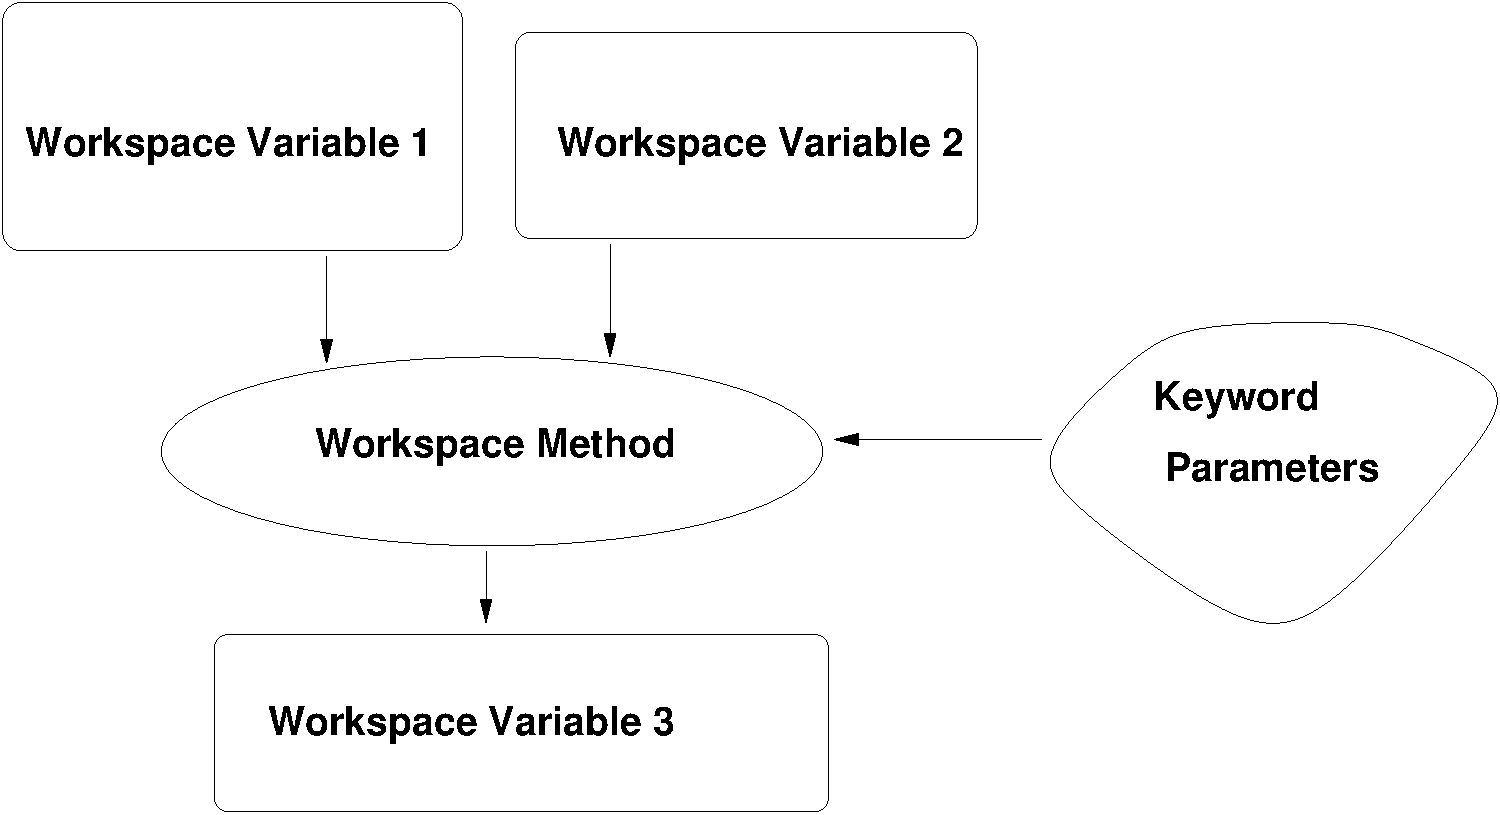
\includegraphics[width=\hsize,draft=false]{method}
    \caption{\emph{Specific}
        workspace methods act on specific workspace variables to
        generate other specific workspace variables. Additional input
        parameters can be specified as keyword parameters in the
        controlfile.}
    \label{fig:method}
  \end{center}
\end{figure}

It is important to note that the controlfile has a fixed and
well-defined syntax. This syntax is understood by the ARTS parser.
The great advantage of this concept is that it is very easy to add
new workspace variables and new workspace methods. The program has
an internal lookup table which lists all workspace methods, as well
as their input variables, output variables, and keyword
parameters. To add a new method, one just has to add an entry to
this lookup table, and write the code for the method itself. No
further changes to the program are necessary. In particular, no
changes to the program logic or to the parser. How such an extension
can be made practically is described in Section \ref{sec:development}.


\levelb{Generic Workspace Methods}
%=================================
\label{sec:concept:generic}

Generic methods (Figure \ref{fig:generic_method}) allow the user of the
program even more freedom than specific methods. A generic method is
for example \verb|VectorReadAscii|, which can be used to read any
workspace variable which is a vector from an ASCII file. For example
\begin{quote}
  \verb|VectorReadAscii(f_mono){"freqeuency_grid.aa"}|
\end{quote}
will read the specified file and generate the workspace variable
\verb|f_grid|.

\begin{figure}
  \begin{center}
    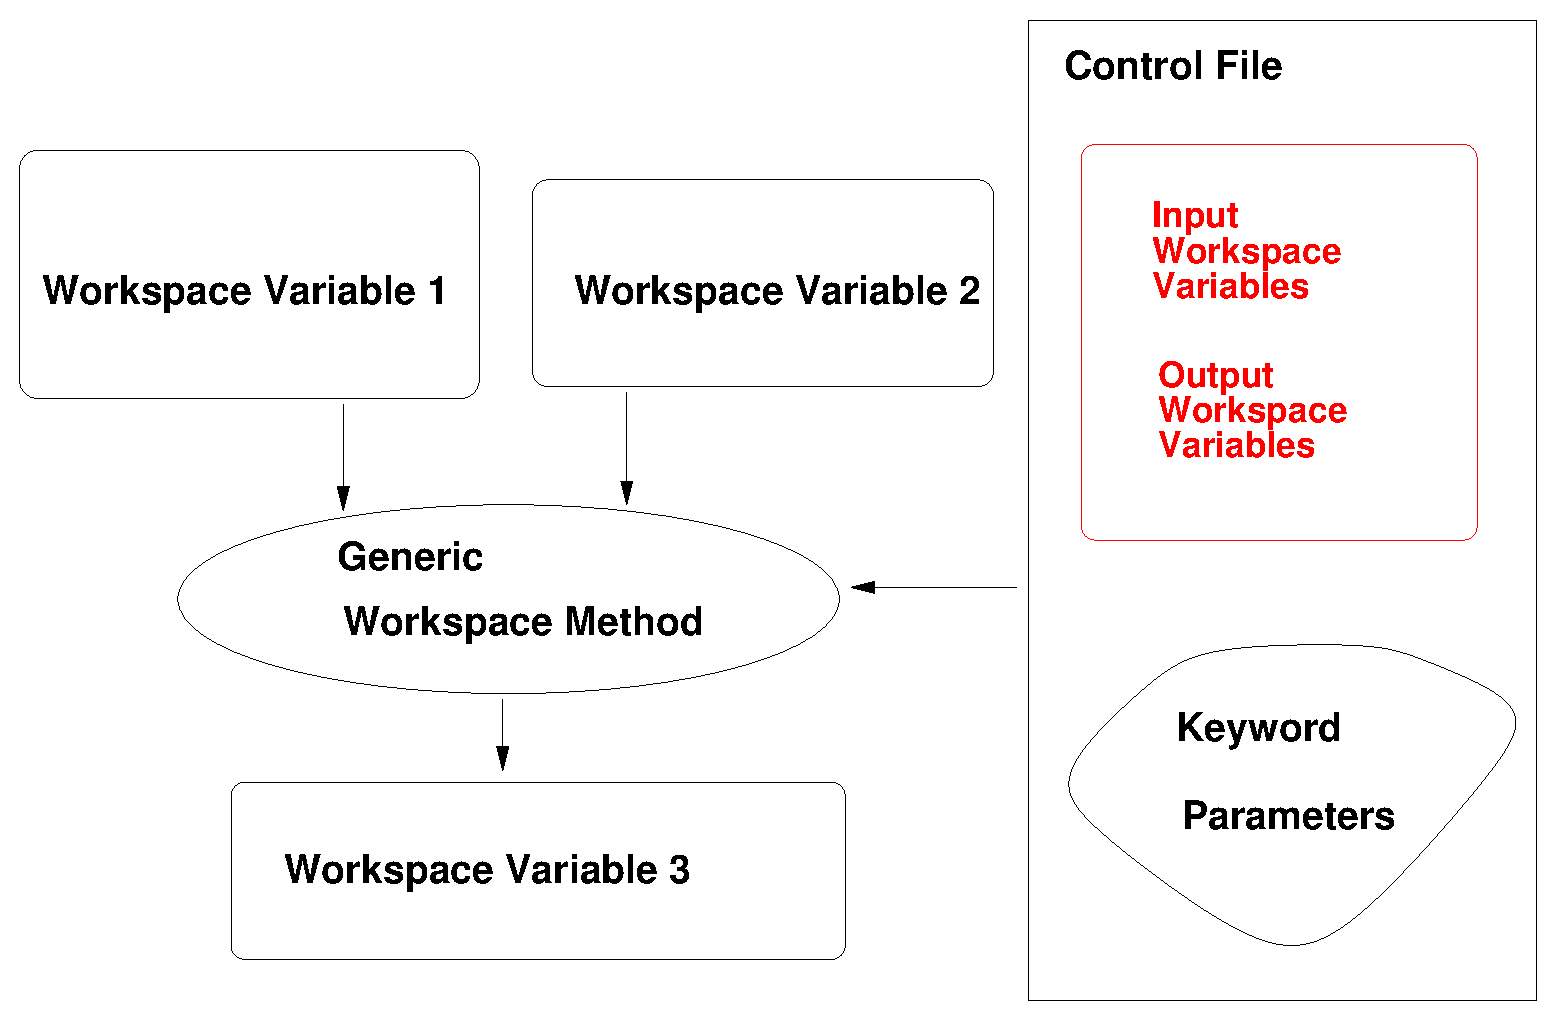
\includegraphics[width=\hsize,draft=false]{generic_method}
    \caption{For \emph{generic}
      workspace methods the workspace variables to act on are
        specified in the controlfile.}
    \label{fig:generic_method}
  \end{center}
\end{figure}

Generic methods are particularly useful for IO operations like in the
example above. No new IO functions are necessary for new workspace
variables, as long as they are of standard types already known to the
program (for example vectors or matrices). 

\levelb{Practical hints}
%=================================
\label{sec:concept:practical}

The subdirectory \verb|examples| of the \verb|doc| directory contains
some example controlfiles. You should study them to learn more about
how the program works. You can also run these controlfiles like this:
\begin{quote}
\begin{verbatim}
  arts absorption_example.arts
\end{verbatim}
\end{quote}
This assumes that you are inside the directory where the controlfiles
are, and that the \verb|arts| executable is in your path.  You can
also run all of the examples, by saying
\begin{quote}
\begin{verbatim}
  make check
\end{verbatim}
\end{quote}

ARTS offers a number of useful command line parameters. In general,
there is a short form and a long form for each parameter. The short
form consists of a minus sign and a single letter, whereas the long
form consists of two minus signs and a descriptive name. To get a full
list, type
\begin{quote}
\begin{verbatim}
  arts -h
\end{verbatim}
\end{quote}
or
\begin{quote}
\begin{verbatim}
  arts --help
\end{verbatim}
\end{quote}
Most useful at the beginning should be the \verb|-d|
(\verb|--describe|), \verb|-m| (\verb|--methods|), \verb|-w|
(\verb|--workspacevariables|), and \verb|-i| (\verb|--input|) flags.
For instance, the \verb|-d| (\verb|--describe|) flag gives you online
documentation for any workspace method or workspace variable. Usage:
\begin{quote}
\begin{verbatim}
  arts -d f_mono
\end{verbatim}
\end{quote}
will print documentation about the workspace variable \verb|f_mono|, which
happens to be the monochromatic frequency grid.

But what methods and variables are available? You can find out by
typing
\begin{quote}
\begin{verbatim}
  arts -m all
\end{verbatim}
\end{quote}
which will list all workspace methods, or by typing 
\begin{quote}
\begin{verbatim}
  arts -w all
\end{verbatim}
\end{quote}
which will list all workspace variables. As you can see, these lists
are quite long. But you can get more specific information:
\begin{quote}
\begin{verbatim}
  arts -m f_mono
\end{verbatim}
\end{quote}
will give you a list of all methods that can generate the workspace
variable \verb|f_mono|. Specific and generic methods are listed
separately. Generic methods are in this case all methods producing a
Vector, since \verb|f_mono| belongs to this group. A similar task is
performed by the \verb|-i| (\verb|--input|) flag, with the difference
that \verb|arts -i f_mono| will list those methods that require
\verb|f_mono| as \emph{input}, whereas \verb|arts -m f_mono| lists
those that produce \verb|f_mono| as output. Finally,
\begin{quote}
\begin{verbatim}
  arts -w absCalc
\end{verbatim}
\end{quote}
will give you all variables required by the method \verb|absCalc|
(the variable \verb|f_mono| happens to be one of them).

Using these command line parameters, it is easy to build up a
controlfile. The trick is, to start at the end. Say you want to
compute absorption coefficients. First of all, you have to find out
in which workspace variable these are stored. Look at the list
produced by \verb|arts -w all|. You can use \verb|arts -d| to look at
some candidates a bit more closely. This way, you will find out that
\verb|abs| is the variable you are looking for.

In the next step, you can use \verb|arts -m abs| to find all methods
that can calculate \verb|abs|. So, you will find the method
\verb|absCalc|. Now you can use \verb|arts -w absCalc| to find out the
required input variables of that method. Then you can use the
\verb|-m| flag again, to find the methods producing these variables,
and so on.

%%% Local Variables: 
%%% mode: latex
%%% TeX-master: "uguide"
%%% End: 

%
% To start the document, use
%  \levela{...}
% For lover level, sections use
%  \levelb{...}
%  \levelc{...}
%
\levela{Theoretical formalism}
 \label{sec:formalism}

%
% Document history, format:
%  \starthistory
%    date1 & text .... \\
%    date2 & text .... \\
%    ....
%  \stophistory
%
\starthistory
  000306 & Written by Patrick Eriksson, partly 
           based on \citet{eriksson:99} and \citet{eriksson:00a}. \\
\stophistory



%
% Symbol table, format:
%  \startsymbols
%    ... & \verb|...| & text ... \\
%    ... & \verb|...| & text ... \\
%    ....
%  \stopsymbols
%
%
%\startsymbols
%  \mpbi   & \verb|y|      & monochromatic pencil beam intensity      \\
%  \f      & \verb|f_mono| & monochromatic frequency                  \\
%  \view   & \verb|za_pencil| & pencil beam zenith angle              \\
%  \iv     & \verb|y|      & vector of monochromatic pencil beam intensities \\
%  \y      & \verb|y|      & spectrum recorded by a sensor            \\
%  \fm     & \verb|-|      & forward model                            \\
%  \fma    & \verb|-|      & atmospheric part of \fm                  \\
%  \fms    & \verb|-|      & sensor part of \fm                       \\
%  \xt     & \verb|-|      & state vector (variables to be retrieved) \\
%  $\xt_r$ & \verb|-|      & atmospheric part of \xt                  \\
%  $\xt_s$ & \verb|-|      & sensor part of \xt                       \\
%  $\xt_\merr$& \verb|-|   & part of \xt\ describing measurement errors   \\
%  \bt     & \verb|-|      & forward model parameter vector           \\
%  $\bt_r$ & \verb|-|      & atmospheric part of \bt                  \\
%  $\bt_s$ & \verb|-|      & sensor part of \bt                       \\
%  $\bt_\merr$& \verb|-|   & part of \bt\ describing measurement errors   \\
%  \Kx     & \verb|k|      & state weighting function matrix          \\
%  \Kb     & \verb|k|      & model parameter weighting function matrix\\  
% \label{symtable:formalism}     
%\stopsymbols



%
% Introduction
%
In this section a theoretical framework for the forward model is
presented. The presentation follows \citet{rodgers:90}, but some
extensions are made, for example, the distinction between the
atmospheric and sensor parts of the forward model is also discussed.
After this chapter was written, C.D. Rodgers published a textbook
\citep{rodgers:00} presenting the formalism in more detail than
\citet{rodgers:90}. Modelling of sensor characteristics is not yet
included in ARTS (this part is so far covered by AMI, see Section
\ref{sec:concept:scope}), but treatment of the sensor is here included
for completness.



\levelb{The forward model}
 \label{sec:formalism:fm}
 
 The radiative intensity, \mpbi, at a point in the atmosphere, $r$, for
 frequency \f\ and traversing in the direction, \view, is dependent
 on a variety of physical processes and continuous variables such as
 the temperature profile, $T$:

 \begin{equation}
   \mpbi = F(r,\f,\view,T,\dots)
 \end{equation} 
 To detect the spectral radiation some kind of sensor, having a finite
 spatial and frequency resolution, is needed, and the observed
 spectrum becomes a vector, \y, instead of a continuous function.
 The atmospheric radiative transfer is simulated by a computer model
 using a limited number of parameters as input, and the forward model,
 \fm, used in practice can be expressed as
 
 \begin{equation}
   \y = \fm(\xt_\fm,\bt_\fm) + \merr(\xt_\merr,\bt_\merr)
  \label{eq:formalism:fm}
 \end{equation}
 where $(\xt_\fm,\bt_\fm)$ and $(\xt_\merr,\bt_\merr)$ together give a
 total description of both the atmospheric and sensor states, and
 \merr\ is the measurement errors. The parameters are divided in such
 way that \xt, the state vector, contains the parameters to be
 retrieved, and the remainder is given by \bt, the model parameter
 vector. The total state vector is
 \begin{equation}
   \xt = \left[ \begin{array}{c} \xt_\fm \\ \xt_\merr \end{array} \right]
 \end{equation}
 and the total model parameter vector is
 \begin{equation}
   \bt = \left[ \begin{array}{c} \bt_\fm \\ \bt_\merr \end{array} \right]
 \end{equation}
 The actual forward model consists of either empirically determined
 relationships, or numerical counterparts of the physical
 relationships needed to describe the radiative transfer and sensor
 effects. The forward model described here is mainly of the latter
 type, but some parts are more based on empirical investigations, such
 as the parameterisations of continuum absorption. 
  
 Both for the theoretical formalism and the practical implementation,
 it is suitable to make a separation of the forward model into two
 main sections, a first part describing the atmospheric radiative
 transfer for pencil beam (infinite spatial resolution) monochromatic
 (infinite frequency resolution) signals \citep{eriksson:99},

 \begin{equation}
   \iv = \fma(\xt_r,\bt_r)
  \label{eq:formalism:fma}
 \end{equation}
 and a second part modelling sensor characteristics,
 \begin{equation}
   \y = \fms(\iv,\xt_s,\bt_s) + \merr(\xt_\merr,\bt_\merr)
  \label{eq:formalism:fms}
 \end{equation}
 where \iv\ is the vector holding the spectral values for the
 considered set of frequencies and viewing angles
 ($\iv^i=I(\f^i,\view^i)$, where $i$ is the vector index), and
 $\xt_\fm$ and $\bt_\fm$ are separated correspondingly, that is,
 $\xt_\fm^T= [\xt_r^T,\xt_s^T]$ and $\bt_\fm^T= [\bt_r^T,\bt_s^T]$.
 The vectors \xt\ and \bt\ can now be expressed as
 \begin{equation}
   \xt = \left[ \begin{array}{c} \xt_r\\ \xt_s \\ \xt_\merr \end{array} \right]
 \end{equation}
 and
 \begin{equation}
   \bt = \left[ \begin{array}{c} \bt_r\\ \bt_s \\ \bt_\merr \end{array}\right],
 \end{equation}
 respectively.

 The subscripts of \xt\ and \bt\ are below omitted as the distinction should be clear by the context. 



\levelb{The sensor transfer matrix} 
 \label{sec:formalism:sensor}
  
 The modelling of the different sensor parts can be described by a
 number of of analytical expressions (see \citet{eriksson:97a}) that
 together makes the basis for the sensor model. These expressions are
 throughout linear operations and it possible, as suggested in
 \citet{eriksson:00a}, to implement the sensor model as a
 straightforward matrix multiplication:
 \begin{equation}
   \y = \Hm \iv + \merr
  \label{eq:formalism:H}
 \end{equation}
 where \Hm\ is here denoted as the sensor transfer matrix.  The matrix
 \Hm\ further incorporate effects of a data reduction and
 the total transfer matrix is then
 \begin{equation}
   \Hm = \Hd \Hs
  \label{eq:formalism:Hs}
 \end{equation}
 as
 \begin{equation}
   \y = \Hd \y' = \Hd (\Hs \iv + \merr') = \Hm \iv + \merr
  \label{eq:formalism:datared}
 \end{equation}
 where \Hd\ is the reduction matrix, \Hs\ the sensor matrix, and $\y'$
 and $\merr'$ are the measurement vector and the measurement errors,
 respectively, before data reduction. The matrices \Hd\ and \Hs\ are
 described in Section \ref{sec:sensor} and \ref{sec:red}, respectively.



\levelb{Weighting functions} 
 \label{sec:formalism:wfuns}

 \levelc{Basics} 
 A weighting function is the partial derivative of the spectrum vector
 \y\ with respect to some variable used by the forward model.  As the
 input of the forward model is divided between \xt\ or \bt, the
 weighting functions are divided correspondingly between two matrices,
 the state weighting function matrix

 \begin{equation}
   \Kx = \frac{\partial \y}{\partial \xt}
  \label{eq:formalism:kx}
 \end{equation}
 and the model parameter weighting function matrix
 \begin{equation}
   \Kb = \frac{\partial \y}{\partial \bt}
  \label{eq:formalism:kb}
 \end{equation}
 For the practical calculations of the weighting functions, it is
 important to note that the atmospheric and sensor parts can be
 seperated. For example, if \xt\ only hold atmospheric and
 spectroscopic variables, \Kx\ can be expressed as

 \begin{equation}
   \Kx = \frac{\partial \y}{\partial \iv}\frac{\partial\iv}{\partial \xt} =
    \Hm\frac{\partial\iv}{\partial \xt}
  \label{eq:formalism:kx2}
 \end{equation}
 This equation shows that the new parts needed to calculate
 atmospheric weighting functions, are functions giving $\partial\iv /
 \partial \xt$ where \xt\ can represent the vertical profile of a
 species, atmospheric temperature, spectroscopic data etc.
% The practical calculation of weighting functions is discussed in
% detail in Sections \ref{sec:wfuns} and \ref{sec:wfuns_sens}.


 \levelc{Transformation between vector spaces}
 
 It could be of interest to transform a weighting function matrix from
 one vector space to another\footnote{This subject is also discussed
   in \citet{rodgers:00} (published after writing this).}. The new
 vector, $\xt'$, is here assumed to be of length $n$ $(\xt' \in
 \msize{n}{1})$, while the original vector, \xt\ is of length $p$
 $(\xt \in \msize{p}{1})$.  The relationship between the two vector
 spaces is described by a transformation matrix $\B$:
  \begin{equation}
    \xt = \B\xt'
  \end{equation}
  where $\B \in \msize{p}{n}$. For example, if $\xt'$ is assumed to be
  piecewise linear, then the columns of $\B$ contain tenth functions,
  that is, a function that are 1 at the point of interest and decreases
  linearly down to zero at the neighbouring points.  The matrix can
  also hold a reduced set of eigenvectors.
    
  The weighting function matrix corresponding to $\xt'$ is
  \begin{equation}
    \K_{\xt'} = \frac{\partial \y}{\partial \xt'}
  \end{equation}
  This matrix is related to the weighting function matrix of \xt\ (Eq.
  \ref{eq:formalism:kx}) as
  \begin{equation}
    \K_{\xt'}
      = \frac{\partial \y}{\partial \xt} \frac{\partial \xt}{\partial \xt'}
      = \frac{\partial \y}{\partial \xt} \B 
      = \Kx \B
  \end{equation}
  Note that
  \begin{equation}
    \K_{\xt'}\xt' = \Kx\B\xt' =  \Kx\xt
  \end{equation}
  However, it should be noted that this relationship only holds for
  those \xt\ that can be represented perfectly by some $\xt'$ (or vice
  versa), that is, $\xt=\B\xt'$, and not for all combinations of \xt\ 
  and $\xt'$.

  If $\xt'$ is the vector to be retrieved, we have that \citep{rodgers:90}
  \begin{equation}
    \xret' = \im(\y,\ct) = \tm(\xt,\bt,\ct)
  \end{equation}
  where \im\ and \tm\ are the inverse and transfer model, respectively.

  The contribution function matrix is accordingly
  \begin{equation}
    \Dy =  \frac{\partial \xret'}{\partial \y}
  \end{equation}
  that is, \Dy\ corresponds to $\K_{\xt'}$, not \Kx.
  
  We have now two possible averaging kernel matrices
  \begin{equation}
    \A_{\xt} 
      = \frac{\partial \xret'}{\partial \xt} 
      = \frac{\partial \xret'}{\partial \y} \frac{\partial \y}{\partial \xt}
      = \Dy \Kx
  \end{equation}
  \begin{equation}
    \A_{\xt'} 
      = \frac{\partial \xret'}{\partial \xt'} 
      = \frac{\partial\xret'}{\partial\y}\frac{\partial\y}{\partial\xt}
      \frac{\partial\xt}{\partial\xt'}
      = \Dy \K_{\xt'}
      = \A_{\xt} \B
  \end{equation}
  where $\A_{\xt} \in \msize{p}{n}$ and $\A_{\xt'} \in \msize{p}{p}$,
  that is, only $\A_{\xt'}$ is square. If $p>n$, $\A_{\xt}$ gives more
  detailed information about the shape of the averaging kernels than
  the standard matrix ($\A_{\xt'}$). If the retrieval grid used is
  coarse, it could be the case that $\A_{\xt'}$ will not resolve all
  the oscillations of the averaging kernels, as shown in
  \citet[][Figure 11]{eriksson:99}.

  
  

    




%%% Local Variables: 
%%% mode: latex
%%% TeX-master: "uguide"
%%% End: 

\part{Algorithm Descriptions}
 %
% To start the document, use
%  \levela{...}
% For lover level, sections use
%  \levelb{...}
%  \levelc{...}
%
\levela{Gas Absorption}
 \label{sec:absorption}


%
% Document history, format:
%  \starthistory
%    date1 & text .... \\
%    date2 & text .... \\
%    ....
%  \stophistory
%
\starthistory
  2001-07-05 & Template created by Stefan Buehler.\\
  2001-10-05 & Line absorption part written, Nikolay Koulev\\
  2001-11-21 & Continuum absorption part written, Thomas Kuhn.\\
\stophistory
%
% Symbol table, format:
%  \startsymbols
%    ... & \verb|...| & text ... \\
%    ... & \verb|...| & text ... \\
%    ....
%  \stopsymbols
%
%
%\startsymbols
%  -- & -- & -- \\
% \label{symtable:wfuns}     
%\stopsymbols

% ============================================================================

% ============================================================================
% TKS definitions for the sections "Continuum Absorption" and 
% "Complete Absorption Models"
%
\def\deni{\rho_{\mbox{\rm i}}}
\def\denl{\rho_{\mbox{\rm l}}}
\def\denli{\rho_{\mbox{\rm l,i}}}
%
\def\imn{{N''}}
\def\ime{\epsilon^{''}_r}
\def\ree{\epsilon^{'}_r}
\def\er{\epsilon_r}
%
\def\bek{\rm b_{\rm 1,k}}
\def\bzk{\rm b_{\rm 2,k}}
\def\bdk{\rm b_{\rm 3,k}}
\def\bvk{\rm b_{\rm 4,k}}
\def\bfk{\rm b_{\rm 5,k}}
\def\bsk{\rm b_{\rm 6,k}}
%
\def\bekp{\rm \widehat{b}_{\rm 1,k}}
\def\bzkp{\rm \widehat{b}_{\rm 2,k}}
\def\bdkp{\rm \widehat{b}_{\rm 3,k}}
\def\bvkp{\rm \widehat{b}_{\rm 4,k}}
\def\bfkp{\rm \widehat{b}_{\rm 5,k}}
\def\bskp{\rm \widehat{b}_{\rm 6,k}}
%
\def\beks{\rm b^*_{\rm 1}}
\def\bzks{\rm b^*_{\rm 2}}
\def\bdks{\rm b^*_{\rm 3}}
\def\bvks{\rm b^*_{\rm 4}}
\def\bfks{\rm b^*_{\rm 5}}
\def\bsks{\rm b^*_{\rm 6}}
%
\def\bekps{\rm \widehat{b^*}_{\rm 1,k}}
\def\bzkps{\rm \widehat{b^*}_{\rm 2,k}}
\def\bdkps{\rm \widehat{b^*}_{\rm 3,k}}
\def\bvkps{\rm \widehat{b^*}_{\rm 4,k}}
\def\bfkps{\rm \widehat{b^*}_{\rm 5,k}}
\def\bskps{\rm \widehat{b^*}_{\rm 6,k}}
%
\def\air{\mbox{air}}
\def\am{\mbox{NH}_3}
\def\hzo{\mbox{H}_2\mbox{O}}
\def\nzo{\mbox{N}_2\mbox{O}}
\def\nz{\mbox{N}_2}
\def\oz{\mbox{O}_2}
\def\co{\mbox{CO}}
\def\coz{\mbox{CO}_2}
\def\clo{\mbox{ClO}}
%
\def\vmroz{VMR_{\mbox{\rm \small O}_{2}}}
%
\def\ptot{P_{\mbox{\rm \small tot}}}
\def\phzo{P_{\mbox{\rm \small H2O}}}
\def\pnz{P_{\mbox{\rm \small N2}}}
\def\poz{P_{\mbox{\rm \small O2}}}
\def\pda{P_{\mbox{\rm \small d}}}
\def\pdair{P_{\mbox{\rm \small air}}}
\def\pan{P_{\mbox{\rm \small air,N2}}}
\def\pcoz{P_{\mbox{\rm \small CO2}}}
%
\def\alphatot{\alpha_{\mbox{\rm \small tot}}} 
\def\alphal{\alpha_{\ell}} 
\def\alphac{\alpha_{\mbox{\small c}}}
\def\alphacs{\alpha_{\mbox{\rm \small c,s}}} 
\def\alphacf{\alpha_{\mbox{\rm \small c,f}}}
%
\def\alphampmotot{\alpha^{\mbox{\rm \small MPM87}}_{\mbox{\small tot}}} 
\def\alphampmmtot{\alpha^{\mbox{\rm \small MPM89}}_{\mbox{\small tot}}} 
\def\alphampmntot{\alpha^{\mbox{\rm \small MPM93}}_{\mbox{\small tot}}} 
\def\alphapwrtot{\alpha^{\mbox{\rm \small R98}}_{\mbox{\small tot}}} 
\def\alphacptot{\alpha^{\mbox{\rm \small CP98}}_{\mbox{\small tot}}} 
%
\def\alphampmol{\alpha^{\mbox{\rm \small MPM87}}_{\mbox{\small $\ell$}}} 
\def\alphampmml{\alpha^{\mbox{\rm \small MPM89}}_{\mbox{\small $\ell$}}} 
\def\alphampmnl{\alpha^{\mbox{\rm \small MPM93}}_{\mbox{\small $\ell$}}} 
\def\alphampml{\alpha^{\mbox{\rm \small MPM}}_{\mbox{\small $\ell$}}} 
\def\alphapwrl{\alpha^{\mbox{\rm \small R98}}_{\mbox{\small $\ell$}}} 
\def\alphacpl{\alpha^{\mbox{\rm \small CP98}}_{\mbox{\small $\ell$}}} 
%
\def\alphampmoc{\alpha^{\mbox{\rm \small MPM87}}_{\rm c}} 
\def\alphampmmc{\alpha^{\mbox{\rm \small MPM89}}_{\rm c}} 
\def\alphampmnc{\alpha^{\mbox{\rm \small MPM93}}_{\rm c}} 
\def\alphapwrc{\alpha^{\mbox{\rm \small R98}}_{\rm c}} 
\def\alphacpc{\alpha^{\mbox{\rm \small CP98}}_{\rm c}} 
%
\def\gamk{\gamma_{\mbox{\rm \small k}}}
\def\gamc{\gamma_{\mbox{\rm \small c}}}
%
\def\ws{w_{\mbox{\rm \small s,k}}}
\def\xs{x_{\mbox{\rm \small s,k}}}
\def\wf{w_{\mbox{\rm \small f,k}}}
\def\xf{x_{\mbox{\rm \small f,k}}}
%
\def\wn{\bar{\nu}}
\def\nucc{\nu_{\mbox{\rm \small c}}}
\def\nucut{\nu_{\mbox{\rm \small cutoff}}}
\def\nuo{\nu_{\mbox{\rm \small 0}}}
\def\nuk{\nu_{\mbox{\rm \small k}}}
%
\def\shape{F(\nu,\nuk)}
\def\shapec{F_{c}(\nu,\nuk)}
\def\shapefp{f_{c}(\nu,+\nuk)}
\def\shapefm{f_{c}(\nu,-\nuk)}
\def\shapefpm{f_{c}(\nu,\pm\nuk)}
\def\inten{S_{\mbox{\rm \small k}}(T)}
\def\inteno{S_{\mbox{\rm \small k}}(300\,K)}
\def\intencp{S_{\mbox{\rm \small 0}}(T)}
%
\def\cx{C_{\mbox{\rm \small x}}}
\def\cs{C_{\mbox{\rm \small H}_{2}\mbox{\rm \small O}}} 
\def\cf{C_{\mbox{\rm N}_{2}}} 
\def\cxo{C^{\mbox{\rm o}}_{\mbox{\rm \small X}}} 
\def\cso{C^{\mbox{\rm o}}_{\mbox{\rm \small H}_{2}\mbox{\rm \small O}}} 
\def\cfo{C^{\mbox{\rm o}}_{\mbox{\rm \small N}_{2}}} 
\def\cao{C^{\mbox{\rm o}}_{\mbox{\rm \small air}}}
\def\cdo{C^{\mbox{\rm o}}_{\mbox{\rm \small d}}}
\def\xx{{\rm n}_{\mbox{\rm \small  x}}} 
\def\xs{{\rm n}_{\mbox{\rm \small  s}}} 
\def\xf{{\rm n}_{\mbox{\rm \small  f}}} 
\def\xd{{\rm n}_{\mbox{\rm \small  d}}}
%
% ============================================================================


                                          

In general there are three types of absorption/emission spectra:
\begin{itemize}
\item sharp lines of finite width
\item aggregations (series) of lines called bands
\item continua extending over a broad range of wavelengths, with
      no single lines in it.
\end{itemize}
This section is therefore firstly devised to give a short theoretical
overview of the absorption quantities which are used in ARTS. The
presentation of the calculation methods within ARTS of these
quantities is the second goal. There are two major subsections which
deal separately with the respective types of spectra regarded by ARTS,
lines and continua.  The second one extends beyond the scope of mere
treatment of the continua and thus gives an integrated view of
continua and spectral lines.

% ================================================================================
% The following section is written by Nikolay Koulev, iup Bremen, nkoulev@uni-bremen.de
% ================================================================================

\levelb{Line Absorption}
%-----------------------
\label{sec:line_absorption}

 
We will introduce here the main concepts concerning
line absorption. The approach, however, does not aim  at the
derivation, but rather at the presentation the following expressions.

Any line is presented by the corresponding profile of the absorption/emission
coefficient as a function of the frequency, in our case that of the
absorption - given by the quantity $\alpha(\nu)$. The latter dependency
is related to other quantities, which express the three
characteristics of a single line uniquely describing it - position,
strength and shape. 
The strength, or better the line intensity, is given by the quantity
$S(T)$, where $T$ is absolute temperature. The shape and the position are expressed through the
line-shape function $F(\nu)$. Thus we have the relation    
\begin{equation}\label{abs_coeff}
  \alpha(\nu)=nS(T)F(\nu)
\end{equation} 
where $n$ is the number density of the absorber, \citet{goodyandyung:89}. The line-shape
function is normalized as follows

\begin{equation}\label{line_shape_norm}
  \int F(\nu)d\nu=1
\end{equation}
The values of $S(T)$ at reference temperature $T_0$ are contained in
spectroscopic databases. The conversion to different temperatures is
done by
\begin{equation}\label{line_intensity}
  S(T)=S(T_0)~\frac{Q(T_0)}{Q(T)}~\frac{e^{-E_f/(kT)}
    - e^{-E_i/(kT)}}{e^{-E_f/(kT_0)} - e^{-E_i/(kT_0)}}
\end{equation}
given the energies $E_f$ and $E_i$ of the two levels between which the
transition occurs as well as the partition function~~$Q(T)$, \citet{rothman:98}. The
databases contain the lower state energy $E_l$ tabulated along with
the $S$ and the transition frequency $\nu$, so that the upper state
energy can be computed by $E_u$=$E_l$+h$\nu$. Partition functions for
all molecular species are also available along with spectroscopic
databases, either in the form of tabulated values for a set
temperatures, or in the form of FORTRAN routines. One can obtain the
total absorption coefficient by adding the absorption of all spectral
lines of all molecular species.

The problem of determining the explicit kind of the line-shape
functions is treated in the following subsection. Another one is
dedicated to the partition functions and their calculation..


\levelc{Line Shape Functions} Up to date there is no way to calculate
the line-shape functions analytically just from the theoretical
expressions of quantum dynamics, statistical physics, and theoretical
mechanics. Certain approximations have to be made to account for
different physical phenomena related to the absorption/emission
process or to suit better the calculation of different parts of the
spectral line.

There are three phenomena which contribute to the line-shape. These
are, in increasing order of importance, the finite lifetime of an
excited state in an isolated molecule, the thermal movement of the gas
molecules, and their collisions with each other. They result in
corresponding effects to the line-shape: natural broadening, Doppler,
and pressure broadening. Of these, the first one is completely
negligible compared to the other two. Nevertheless, we will pay a
special attention to the natural broadening because its implications
are of a conceptual importance for the broadening processes.

The spectral line shape can be derived in the case of natural
broadening from basic physical considerations and a well-known Fourier
transform theorem from the time to the frequency domain, \citet{thorne:99}. If we
consider classically the spontaneous decay of the excited state of
two-level system in the absence of external radiation, then population
$n$ of these level decreases according to
\begin{equation}\label{spon_decay_diff}
  \frac{dn(t)}{dt} = -A\,n(t)
\end{equation}
where $A$ is Einstein A coefficient, which equation can also be
interpreted as the rate of the spontaneously emitted photons because
of decay. This relation is more usefully in this case to be written in
the following manner 
\begin{equation}\label{spon_decay_exp}
  n(t)=n(0)~e^{-At}=n(0)e^{-t/\tau}
\end{equation}
where $ \tau$ is the mean lifetime of the excited state. Thus the
number of spontaneously emitted photons and in this way the flux of
the emitted radiation then will be proportional to $n$. Therefore we
can write for the flux $L$ that
\begin{equation}\label{flux}
  L(t)=L(0)~e^{-t/ \tau}=L(0)~e^{-\gamma t}
\end{equation}
By the afore mentioned theorem, multiplying in the time domain by
$e^{-\gamma t}$ is equivalent to convolving in the frequency domain
with a function $1/[\nu^2 - (\gamma/4\pi)^2]$. Accordingly the line
profile of a spectral line at frequency $ \nu_0$ as a normalized
line-shape function will be, as difined in \citet{thorne:99},
\begin{equation}\label{natural_lorentz}
  F(\nu)=\frac{1}{\pi}\frac{\gamma/4\pi}{(\nu - \nu_0)^2 + (\gamma/4\pi)^2}
\end{equation}
This gives a bell-shaped profile and the function itself is called
Lorentzian. The dependence on the position of the line is apparent
through $\nu_0$, that is why some authors prefer to denote the
function by $F(\nu,\nu_0)$.  The result is important because of two
major reasons.  Firstly, without the natural broadening the line would
be the delta function~$\delta (\nu - \nu_o)$, as pointed out in
\citet{bernath:95}. So the spontaneous decay of the excited state is
responsible for the finite width and the certain shape of the
line-shape function. Secondly, the Lorentzian type of function comes
significantly into play when explaining some of the other broadening
effects or the complete picture of the broadened line, \citet{thorne:99}.

The second effect, Doppler broadening, is important for the upper
stratosphere and mesosphere for microwave frequencies. The line-shape
follows the velocity distribution of the particles. Under the conditions
of thermodynamic equilibrium, we have  a probability distribution for
the relative velocity $u$ between the gas molecule and the observer 
of Maxwell type 
\begin{equation}\label{maxwell_distribution}
  p(u)=\sqrt{\frac{m}{2\pi kT}}~~exp~\left[-\frac{mu^2}{2kT}\right]
\end{equation}
where $m$ is the mass of the molecule. Using then the formula for the
Doppler shift for the non-relativistic region~~  $\nu$- $\nu_0$ =
$\nu_0$$u$ / $c$ , one can easily derive the line-shape function, \citet{bernath:95}, 
\begin{equation}
 F_D(\nu)=\frac{1}{\gamma_D\sqrt{\pi}}~~exp~\left[-\left(\frac{\nu - \nu_0}{\gamma_D}\right)^2\right]
\end{equation}
where the quantity $\gamma_D$ is called Doppler line width and equals
\begin{equation}
 \gamma_D=\frac{\nu}{c}\sqrt{\frac{2kT}{m}}
\end{equation}
In contrast to the afore mentioned line-shape function for the natural
broadening the Doppler broadening is expressed by a Gaussian
line-shape function $F(\nu)$. The Doppler line width $\gamma_D$ is so
defined that it is equal to the half width at half of the maximum
(HWWM) of the line-shape function. The same way of notating is used
for all other width parameters $\gamma_{xy}$ below.

It can be said without any exaggeration that the pressure broadening
effect is the most complicated one among the others and still
represents a complex theoretical task to be tackled, and is in the
same time of major experimental importance. So far, there is no way to
calculate analytically from the basics the profile of a pressure, or
collisional, line through a single approach near the line center as
well as in the far wing region. The various approximations, which are
therefore used, are immanently limited to the certain line regions
they deal with.  The most popular among these approximations is the
{\it{impact~approximation}} which postulates that the duration of the
collisions of the gas particles is very small compared to the average
time between the collisions. Lorentz was the first to achieve a result
exploiting this approach, the Lorentz line-shape function:
\begin{equation}\label{pressure_lorentz}
 F_L(\nu)=\frac{\gamma_L}{\pi}\frac{1}{(\nu-\nu_0)^2+\gamma_L^2}
\end{equation}
where $\gamma_L$ is the Lorentz line width, \citet{thorne:99}. As one
can see, the result Eq.\,\ref{pressure_lorentz} is pretty similar to
Eq.\,\ref{natural_lorentz} but the specific line parameters $\gamma$
and $\gamma_L$ make them differ significantly in the corresponding
frequency regions of interest. For atmospheric pressures $\gamma_L$ is
much greater and because of that, of experimental
significance in contrast to $\gamma$.\\
Elaborating the model of Lorentz, van Vleck and Weisskopf made a
correction to it, \citet{vanvleck:45},particularly for the microwave
region:
\begin{equation}\label{eq:vvw}
 F_{VVW} (\nu)=\left(\frac{\nu}{\nu_0}\right)^2\frac{\gamma_L}{\pi}
 \left[\frac{1}{(\nu-\nu_0)^2+\gamma_L^2}+\frac{1}{(\nu+\nu_0)^2+\gamma_L^2}\right]
\end{equation}
which can be reduced to a Lorentzian for $(\nu-\nu_0) << \nu_0$ and $0
<< \nu_0$. Except for the additional factor $(\nu/\nu_0)^2$ ,
$F_{VVW}$ can be regarded as the sum of two $F_L$, or respectively
lines, one with its center frequency at $\nu_0$, the other at
$-\nu_o$.

The van Vleck and Huber lineshape \citep{vanvleckhuber:77} is similar
to Eq.\,\ref{eq:vvw}, except for the factor $(\nu/\nu_0)^2$ which is
replaced by $(\nu * \tanh(h*\nu/(2kT)))/(\nu_0 *
\tanh(h*\nu_0/(2kT)))$, with $k$ the Boltzmann constant, $h$ the Planck
constant, and $T$ the atmospheric temperature (the denominator is
actually a consequence of the line strength definition in the
spectroscopic catalogs). The lineshape Eq.\,\ref{eq:vvw} with this
factor can be used for the entire frequency range, since
the microwave approximation: $\tanh(x) = x$, that leads to the factor
$(\nu/\nu_0)^2$, is not made.

The combined picture of a simultaneously Doppler and pressure
broadened line is the next step of the approximations development. The
line-shape function has to approximated in this case by the Voigt line-shape
function 
\begin{equation}\label{voigt}
 F_{Voigt}(\nu,\nu_0)= \int F_L(\nu,\nu')~F_D(\nu',\nu_0)~d\nu'
\end{equation}
though there's no strict justification for its use - the two processes
are assumed to act independently, which in reality is not the
fact. Regardless of this flaw, it is the only way up to date to model
the combination of the broadening processes. The integral in Eq.\,\ref{voigt}
can not be computed analytically, so certain approximation algorithms
must be used.


Another possibility would be the combination of the last two equations
Eq.\,\ref{eq:vvw} and Eq.\,\ref{voigt}. The respective result then will be 
\begin{equation}\label{voigt_mirror}
 F_S=\left(\frac{\nu}{\nu_0}\right)^2~[F_{Voigt}(\nu,\nu_0)+F_{Voigt}(\nu,-\nu_0)]
\end{equation}
The advantage of such a model is that it behaves like a van
Vleck-Weisskopf line-shape function in the high pressure limit and
like a Voigt one in the low pressure limit. There is one important
caveat to the equation Eq.\,\ref{voigt_mirror}: it has to be made sure that the
algorithm that is used to compute the Voigt function really produces a
Lorentz line in the high pressure limit. Another point of significance
is the demand that the model yields meaningful results far from the
line center, since the line center from the ``mirror'' line at
-$\nu_0$ is situated approximately 2$\nu_0$ away from the frequency
$\nu_0$ of computation. The algorithm of \citet{Drayson:76} and
\citet{Oliveiro:77} was explicitly checked to satisfy both
requirements, while this was found to be not true for some other
algorithms, commonly used for Voigt-shape computation. In particular,
the it is not true for the Hui-Armstrong-Wray Formula, as defined in
\citet{hui:78} and in Equation 2.60 of \citet{pwr:93}. So, provided
the stated above is fulfilled, the $F_S$ line shape gives a smooth
transition from high tropospheric pressures to low stratospheric ones,
and should be valid near the line centers throughout the microwave region.






\levelc{Partition Functions}

The treatment of the partition functions is directly related to the molecular
energy states and their statistical distribution during the
radiation process. 

In any case of spectroscopic interest the free molecules of a gas are
not optically thick at all frequencies, so the radiation energy is not
represented by blackbody radiation. The most common assumption made,
which is sufficient in the case of tropospheric and low stratospheric
research, is the {\textit{local thermodynamic equilibrium}\nocorr} or
{\textit{LTE }\nocorr}. According to it, it's possible to find a common temperature,
which may vary from place to place, that fits the Boltzmann energy
population distribution and the Maxwell velocities distribution.
This practically means, that under $LTE$ the collisional processes
must be of greater importance than radiative ones. In other words,
an excited state must have a higher probability of de-excitation by
collision than by spontaneous radiation. This is the important
factor which makes natural broadening differ quantitatively so much
from the pressure (collisional) one, though both are described
qualitatively almost identically by Lorentzian line- shape
functions.

According to the Maxwell-Boltzmann distribution law, in $LTE$ the total number
of gas particles $N_n$  in a state $E_n$ is given by 
\begin{equation}\label{maxwell_distribution}
 N_n=N_0\frac{g_n}{g_0}e^{-E_n/kT}
\end{equation}
where $N_0$ is particle number in the ground state, and $g_n$, $g_o$
are the statistical weights (degeneracies) of the $n-$state and the
ground state, \citet{gordyandcook:70}. Thus the total particle number $N$ is given by
\begin{equation}\label{total_part_number}
 N=\frac{N_0}{g_0}\sum_{n=0}^\infty g_n~e^{-E_n/kT}=\frac{N_0}{g_0}~Q(T)
\end{equation}
The quantity $Q(T)$ is the {\it{partition function}\nocorr} of the
gas, which generally speaking describes the energy states distribution
of the gas particles. 

The partition function for a perfect gas molecule can be represented
by the product of the {\it{translational}\nocorr} and the
{\it{internal}\nocorr} partition functions, as defined in \citet{herzberg:45},
\begin{equation}\label{partition_f_general}
 Q  =  Q_{tr}~Q_{int}
\end{equation}
bearing in mind that the respective energies, translational and
internal, are independent of each other. The first quantity $Q_{tr}$ accounts
for the distribution of the translational energy of the gas particles
- it takes into account that the translational velocities of the
particles fulfill the Maxwell distribution. The quantity, however,
which we are interested in in (3.3) is the {\it{internal}\nocorr}
partition function (or the {\it{total internal partition  function}\nocorr}
 because the transitions between the discrete
internal energy states are responsible for the absorption or emittance
of radiation. Accordingly $Q_{int}$ describes the
distribution of energy among the internal energy states of the gas
particles.

The internal partition function for free gaseous molecules is a
function of the electronic, the vibrational, the rotational, and the
nuclear spin states. An approximation is used in
\citet{gordyandcook:70} in order to display the individual
contribution explicitly
\begin{equation}\label{int_partition}
 Q_{int}=Q_e~Q_v~Q_r~Q_n
\end{equation}
and thus the interaction between these various states is neglected.
For practically all polyatomic molecules the excited electronic states
are entirely negligible to those of the ground states, i.e. $Q_e=1$ .
Only for the very few polyatomic molecules with a multiplet ground
state ($NO_2$ , $ClO_2$ , and free radicals) has the
electronic contribution to be considered.\\
If we neglect the anharmonicities, the vibrational partition function,
with vibrational energy levels measured with respect to the ground
state for the {\it harmonic oscillator}, is acording \citet{herzberg:45}
\begin{equation}\label{vib_partition}
 Q_v=\left(\sum_{\nu_1}e^{-\nu_1 h\omega_1/kT}\right)\left(\sum_{\nu_2}e^{-\nu_2 h\omega_2/kT}\right)...
\end{equation}
where $\nu_1$, $\nu_2$,..., the vibrational quantum numbers, can each
have the values 0,1,2,... and $\omega_1$, $\omega_2$,..are the
frequencies of the fundamental modes of vibration. The summation is
taken over all values of $\nu_1$, $\nu_2$,..., and each fundamental
mode is counted separately. This result is valid for non-degenerate
vibrations. If we use the simple expression for geometric progression
\begin{equation}\label{geom_progression}
 \sum_{\nu_i}e^{-\nu_i h\omega_i/kT}=\frac{1}{1-e^{h\omega_i/kT}}
\end{equation}
and the degeneracies $d_1$, $d_2$,... of the fundamental modes, we get
finally for the vibrational partition function
\begin{equation}\label{vib_partition_fin}
Q_v=\left(1-e^{h\omega_1/kT}\right)^{-d_1}\left(1-e^{h\omega_2/kT}\right)^{-d_2}...
\end{equation}

The rotational partition function looks differently for the different
symmetry types of molecules.
For diatomic and linear  polyatomic molecules with no center of
symmetry the corresponding expression is, as defined in \citet{gordyandcook:70}
\begin{eqnarray}\label{rot_partition}
Q_r & = & \sum_{J=0}^\infty (2J+1)e^{-hBJ(J+1)/kT}\nonumber\\
   & = & \frac{kT}{hB}+\frac{1}{3}+\frac{1}{15}\frac{hB}{kT}+\frac{4}{315}\left(\frac{hB}{kT}\right)^2+...\nonumber\\
   & \cong & \frac{kT}{hB}
\end{eqnarray}
For {\it{ rigid symmetric-}}, {\it{asymmetric-}}, and {\it{spherical}} top molecules there are also
other factors to be taken into consideration, such as the
spatial structure of the molecules, nuclear spin, inversion and
internal rotation. The general expression in the case of a 
{\it{ rigid symmetric-}} top molecule according \citet{herzberg:45}
is
\begin{equation}\label{rot_partition_symtop}
Q_r  =  \frac{1}{\sigma}\sum_{J=0}^\infty \sum_{K=-J}^{J}(2J+1)~e^{-h[BJ(J+1)+(A-B)K^2]/kT}
\end{equation}
where $\sigma$ is measure of the degree of symmetry. The usual
symmetric top has $C_3$ or $C_{3\nu}$ symmetry, therefore $\sigma$ = 3. To a good
approximation, the summation above can expressed as in \citet{gordyandcook:70}
\begin{equation}\label{rot_partition_top_appro}
Q_r  = 
\frac{1}{\sigma}\left[\left(\frac{\pi}{B^2A}\right)\left(\frac{kT}{h}\right)^3\right]^{1/2}=
\frac{5.34\times 10^6}{\sigma}\left(\frac{T^3}{B^{2}A}\right)^{1/2}
\end{equation}
For an  {\it{asymmetric}} top the formula would then be 
\begin{equation}\label{rot_partition_asymtop}
Q_r = \frac{5.34\times 10^6}{\sigma}\left(\frac{T^3}{ABC}\right)^{1/2}
\end{equation}
and for a {\it{spherical}} top, using the current notation of
\citet{gordyandcook:70} in the respective expression in \citet{herzberg:45},
\begin{equation}\label{rot_partition_sphetop}
Q_r = \frac{5.34\times 10^6}{\sigma}\left(\frac{T^3}{A^3}\right)^{1/2}
\end{equation}








\levelc{Line Catalogs} There are several spectroscopic catalogs
implemented in ARTS: HITRAN, JPL, MYTRAN, and the ARTS inherent
catalog format.

Special attention will be paid here only to the inherent format in ARTS.
To keep track with the changes in the catalog format, every catalog file
must start with $ARTSCAT-x$ , where for current version $x=2$.  Files
with different or missing version will be rejected. The current
version is stored in the private member variable mversion. It can be
read with the member function Version, which returns a String `ARTSCAT-x'.
After the version tag (ARTSCAT-x), ARTS outputs the number of lines
when catalog files are written. This number is not used by reading
routines, though.

The line catalog should not have any fixed column widths because the
precision of the parameters should not be limited by the format. The
catalog can then be stored in principle as binary or ASCII, though
currently are implemented only ASCII files. In the ASCII version
the columns are separated by one or more blanks. The line format is
then specified by only the order and the units of the columns. As the
catalog entry for each transition can be quite long, it can be broken
across lines in the ASCII file. Each new transition is marked with an
`@' character.  The first column will contain the species and isotope,
following the naming scheme described below. Scientific notation is
allowed, e.g. 501.12345e9.  Note that starting with ARTSCAT-2, the
intensity is per molecule, i.e., it does not contain the isotopic
ratio. This is similar to JPL, but different to HITRAN.  The line
format is:

\begin{verbatim}

Col  Variable                     Label    Unit     
-----------------------------------------------      
 0   `@'                         ENTRY        -     
 1   name                         NAME        -     
 2   center frequency                F       Hz     
 3   pressure shift of F           PSF    Hz/Pa    
 4   line intensity                 I0   m^2/Hz     
 5   reference temp. for I0       T_I0        K
 6   lower state energy           ELOW        J    
 7   air broadened width          AGAM    Hz/Pa     
 8   self broadened width         SGAM    Hz/Pa
 9   AGAM temp. exponent          NAIR        -     
10   SGAM temp. exponent         NSELF        - 
11   ref. temp. for AGAM, SGAM   T_GAM        K
12   number of aux. parameters   N_AUX        -
13   auxiliary parameter          AUX1        -
14   ... 
15   error for F                    DF       Hz
16   error for I0                  DI0        %
17   error for AGAM              DAGAM        %
18   error for SGAM              DSGAM        %
19   error for NAIR              DNAIR        %
20   error for NSELF            DNSELF        %
21   error for PSF                DPSF        %
22   quantum number code         QCODE           
23   lower state quanta         QLOWER            
24   upper state quanta         QUPPER            
25   information source of F                      IF
26   information source of I0                     II0
27   information source of line width variables   ILW
28   information source of pressure shift         IPSF
29   information source of auxiliary parameters   IAUX
\end{verbatim}
The parameters 0-12 must be present, the others can be missing, since
they are not needed for the calculation. For the error fields (15-21),
a~$-1$ means that no value exists. Fields 22-29 are strings inside quotes
\verb ""  for maximum flexibility.\\
Thus a valid ARTS line file would be:
\begin{verbatim}
ARTSCAT-2 2
@ CH4-211 1011349857.063 0 2.96070344144819e-27 296
2183.6851 13314.2468393782 21302.7949430052 0.75 0.75 296 0
@ O3-666 1088246622.54 0 2.82913939200384e-22 296
522.5576 21361.9693734024 27723.2206411054 0.76 0.76 296 0
\end{verbatim}
Some species need special parameters that are not needed by other
species (for example overlap coefficients for $O_2$). In the case of
oxygen two parameters are sufficient to describe the overlap, but
other species, e.g., methane, may need more coefficients. The default
for \texttt{N\_AUX} is zero. In that case, no further \texttt{AUX}
fields are present.







\levelc{Species specific data}

The following part treats the species related data in ARTS - all
currently implemented species with the respective molecular masses,
isotopic ratios, partition functions, and the sources for this
information. 

Table \ref{table:impl_secies} lists the implemented species in ARTS.
The first row gives the ARTS molecule name, the second the ARTS
isotope name (these two identify the species within ARTS). The third
row gives the number of this species in the MYTRAN catalog, the fourth
the one used in HITRAN96, and the fifth the corresponding tag numbers
of the JPL00 catalog.



\begin{longtable}{lllll}
 K & K & K & K & K \kill
%
% --------------------- only begin of table ------------------------------

 \hline
 {\it ARTS }& {\it ARTS }& {\it MYTRAN}& {\it HITRAN}& {\it JPL00}\\
 {\it Name}& {\it Isotope}& {\it Tag}& {\it Tag}& {\it Tag}\\ 
 \hline
 \endfirsthead
% --------------------- every page begin of table ------------------------
 \hline
 {\it ARTS }& {\it ARTS }& {\it MYTRAN}& {\it HITRAN}& {\it JPL00}\\
 {\it Name}& {\it Isotope}& {\it Tag}& {\it Tag}& {\it Tag}\\ 
 \hline
 \endhead
% --------------------- every page end of table ------------------------
 K & K & K & K & K \kill
 \hline
 \caption[]{(continued)}\\
 \endfoot
% --------------------- only end of table ------------------------------
 K & K & K & K & K \kill
 \hline
 \caption{Implemented species in ARTS} 
 \label{table:impl_secies}
 \endlastfoot
% --------------------- body of table ---------------------------------- 

 

  H2O& 161&  11&    11&  18003, 18005\\
     & 181&  12&    12&  20003\\
     & 171&  13&    13&  19003\\
     & 162&  14&    14&  19002\\
     & 182&  -1&    15&  21001\\
     & 172&  -1&    16&       \\
     & 262&  -1&    -1&  20001\\
     &SelfContStandardType&             -1&  -1 & \\      
     &ForeignContStandardType&          -1&  -1 & \\  
     &ForeignContMaTippingType&         -1&  -1 & \\      
     &ContMPM93&                        -1&  -1 & \\      
     &SelfContCKD24&                    -1&  -1 & \\      
     &ForeignContCKD24&                 -1&  -1 & \\ 
     &ForeignContATM01&                 -1&  -1 & \\         
     &CP98&                             -1&  -1 & \\      
     &MPM87&                            -1&  -1 & \\      
     &MPM89&                            -1&  -1 & \\      
     &MPM93&                            -1&  -1 & \\      
     &PWR98&                            -1&  -1 & \\  


\hline                  
  CO2& 626&  21&    21&\\
     & 636&  22&    22&\\
     & 628&  23&    23&  46013\\
     & 627&  24&    24&  45012\\
     & 638&  25&    25&\\
     & 637&  26&    26&\\
     & 828&  27&    27&\\
     & 728&  28&    28&\\
     &SelfContPWR93&    -1&-1&\\
     &ForeignContPWR93& -1&-1&\\
\hline                  
  O3& 666&  31&    31&  48004, 48005,\\
    &    &    &      &  48006, 48007,\\
    &    &    &      &  48008\\
    & 668&  32&    32&  50004, 50006\\
    & 686&  33&    33&  50003, 50005\\
    & 667&  34&    34&  49002\\
    & 676&  35&    35&  49001\\
\hline                  
  N2O& 446&  41&    41&  44004, 44009,\\
     &    &    &      &  44012\\
     & 456&  42&    42&  45007\\
     & 546&  43&    43&  45008\\
     & 448&  44&    44&  46007\\
     & 447&  -1&    45&\\
\hline                   
  CO&   26&  51&    51&  28001\\
    & 36&  52&    52&  29001\\
    & 28&  53&    53&  30001\\
    & 27&  -1&    54&  29006\\
    & 38&  -1&    55&\\
    & 37&  -1&    56&\\
\hline                  
  CH4& 211&  -1&    61&\\
     & 311&  -1&    62&\\
     & 212&  -1&    63&  17003\\
\hline                  
  O2& 66&  71&    71&  32001, 32002\\
    & 68&  72&    72&  34001\\
    & 67&  73&    73&  33002\\
    &SelfContStandardType&   -1        &-1&     \\
    &SelfContMPM93&          -1        &-1&     \\
    &SelfContPWR93&          -1        &-1&     \\
    &PWR98&                  -1        &-1&     \\ 
    &PWR93&                  -1        &-1&     \\
    &PWR88&                  -1        &-1&     \\  
    &MPM93&                  -1        &-1&     \\
    &MPM92&                  -1        &-1&     \\
    &MPM89&                  -1        &-1&     \\
    &MPM85&                  -1        &-1&     \\
\hline                  
  NO& 46&  81&    81&  30008\\
    & 56&  -1&    82&\\
    & 48&  -1&    83&\\
\hline                  
  SO2& 626&  91&    91&  64002, 64005\\
     & 646&  92&    92&  66002\\
     & 636&  93&    -1&  65001\\
     & 628&  94&    -1&  66004\\
\hline                  
  NO2& 646&  101&   101&  46006\\
\hline                  
  NH3& 4111&  111&   111&  17002, 17004\\
     & 5111&  112&   112&  18002\\
     & 4112&  -1&    -1&  18004\\
\hline                  
  HNO3& 146&  121&   121&  63001, 63002,\\
      &    &     &      &  63003, 63004,\\
      &    &     &      &  63005, 63006\\
\hline                  
  OH& 61&  131&   131&  17001\\
    & 81&  132&   132&  19001\\
    & 62&  133&   133&  18001\\
\hline                  
  HF& 19&  141&   141&  20002\\
    & 29&  -1&    -1&  21002\\
\hline                  
  HCl&15&  151&   151&  36001\\
     &17&  152&   152&  38001\\
     &25&  -1&    -1&  37001\\
     &27&  -1&    -1&  39004\\
\hline                  
  HBr& 19&  161&   161&  80001\\
     & 11&  162&   162&  82001\\
\hline                  
  HI& 17&  -1&   171&\\
\hline                  
  ClO& 56&  181&   181&  51002, 51003\\
     & 76&  182&   182&  53002, 53006\\
\hline                  
  OCS& 622&  191&   191&  60001\\
     & 624&  192&   192&  62001\\
     & 632&  193&   193&  61001\\
     & 822&  194&   194&  62002\\
     & 623&  195&   195&       \\
\hline                  
  H2CO& 1126&  201&   201&  30004\\
      & 1136&  202&   202&  31002\\
      & 1128&  203&   203&  32004\\
      & 1226&  -1&    -1&  31003\\
      & 2226&  -1&    -1&  32006\\
\hline                  
  HOCl& 165&  211&   211&  52006\\
      & 167&  212&   212&  54005\\
\hline                  
  N2& 44&  -1&   221&\\
    &SelfContMPM93&             -1      &-1     \\
    &SelfContPWR93&             -1      &-1     \\
    &SelfContStandardType&      -1      &-1     \\
    &SelfContBorysow&           -1      &-1     \\
    &DryContATM01&              -1      &-1     \\


\hline                  
  HCN& 124&  231&   231&  27001, 27003\\
     & 134&  232&   232&  28002\\
     & 125&  233&   233&  28003\\
     & 224&  -1&    -1&  28004\\
\hline                  
  CH3Cl& 215&  241&   241&  50007\\
       & 217&  242&   242&  52009\\
\hline                  
  H2O2& 1661&  251&   251&  34004\\
\hline                  
  C2H2& 1221&  -1&   261&\\
      & 1231&  -1&   262&\\
\hline                  
  C2H6& 1221&  -1&   271&\\
\hline
  PH3& 1111&  281&   281&  34003\\
\hline                  
  COF2&  269&  291&   291&  66001\\
\hline                  
  SF6& 29&  -1&   301&\\
\hline                  
  H2S& 121&  311&   311&  34002\\
     & 141&  -1&   312&\\
     & 131&  -1&   313&\\
     & 122&  -1&    -1&  35001\\
\hline                  
  HCOOH& 1261&  321&   321&  46005\\
       & 1361&  -1&    -1&  47002\\
       & 2261&  -1&    -1&  47003\\
       & 1262&  -1&    -1&  47004\\
\hline                  
  HO2& 166&  331&   331&  33001\\
\hline                  
  O& 6&  341&   341&  16001\\
\hline                  
  ClONO2& 5646&  351&   351&  97002\\
        & 7646&  352&   352&  99001\\
\hline                  
  NO+& 46&  -1&   361&  30011\\
\hline                  
  OClO& 656&  431&    -1&  67001\\
      & 676&  432&    -1&  69001\\
\hline                  
  BrO& 96&  401&    -1&  95001\\
     & 16&  402&    -1&  97001\\
\hline                  
  H2SO4& 126&  481&    -1&  98001\\
\hline                  
  Cl2O2& 565&  491&    -1&  102001\\
       & 765&  492&    -1&  104001\\
\hline                  
  HOBr & 169&  371&    371&  96001\\
       & 161&  372&    372&  98002\\
\hline                  
  C2H4 & 221&  381&    371&       \\
       & 231&  382&    372&       \\
\hline                  
CH3CN & 211124&   &        & 41001 \\
      & 311124&   &        & 42006 \\
      & 211134&   &        & 42007 \\
      & 211125&   &        & 42001 \\
      & 211224&   &        & 42008 \\
\hline                  
  HNC & 142&      &        & 27002 \\
  HNC & 143&      &        & 28005 \\
  HNC & 152&      &        & 28006 \\
  HNC & 242&      &        & 28007 \\
\hline                  
liquidcloud& MPM93&  &     &       \\
\hline                  
icecloud& MPM9&      &     &       \\
\hline                  
rain     & MPM93 &   &     &       \\
\end{longtable}
 

Table \ref{table:isoratio} gives an overview of the isotopic ratios
and their sources, and the molecular mass of the species used in used
in ARTS.  The isotopic ratio of the species was in general taken from
HITRAN00, even for species where JPL00 and HITRAN00 give isotopic
ratios. 
Species not present in HITRAN00 were extracted from JPL00.
JPL00 isotopic ratios are normalized to 1 for some molecules, for
these cases, the HITRAN00 isotopic ratio of the major isotope was used
to scale the JPL00 isotopic ratio to relative number.

As in \ref{table:impl_secies} the first two columns give the ARTS
molecule name and  the ARTS isotope name. The next two ones give the
isotopic ratio and the source it is taken from respectively. An entry
of 1 corresponds to HITRAN00, 2 to JPL00, 3 to JPL00 multiplied with
the maximum abundance of this molecule in HITRAN. The
last column contains the molecular masses of the isotopes. An entry of -1 is
prescribed to the continuum tags. 



\begin{longtable}{lllll}
 K & K & K & K & K   \kill
%
% --------------------- only begin of table ------------------------------
 \hline
 {\it ARTS }& {\it ARTS }& {\it Isotopic }& {\it Isotopic Ratio }&{\it Mass}\\
 {\it Name }& {\it Isotope }& {\it Ratio }& {\it Source }         &      \\ 
 \hline
 \endfirsthead
% --------------------- every page begin of table ------------------------
 \hline
 {\it ARTS }& {\it ARTS }& {\it Isotopic }& {\it Isotopic Ratio }&{\it Mass}\\
 {\it Name }& {\it Isotope }& {\it Ratio }& {\it Source }         &      \\  
 \hline
 \endhead
% --------------------- every page end of table ------------------------
 K & K & K & K & K   \kill
 \hline
 \caption[]{(continued)}
 \endfoot
% --------------------- only end of table ------------------------------
 K & K & K & K & K   \kill
 \hline
 \caption{Isotopic ratios within ARTS, source of the ratios and molecular mass}
 \label{table:isoratio}
 \endlastfoot
% --------------------- body of table ---------------------------------- 
  

  H2O& 161&  0.99731702&  1&18\\
     & 181&  0.00199983&  1&20\\
     & 171&  0.00037200&  1&19\\
     & 162&  0.00031069&  1&19\\
     & 182&  6.23003E-07& 1&21\\
     & 172&  1.15853E-07& 1& 20\\
     & 262&  2.2430204E-08&  3&20\\
     &SelfContStandardType&     -1    &-1    &-1     \\
     &ForeignContStandardType&  -1    &-1    &-1     \\
     &ForeignContMaTippingType& -1    &-1    &-1     \\
     &ContMPM93&                -1    &-1    &-1     \\
     &SelfContCKD24&            -1    &-1    &-1     \\
     &ForeignContCKD24&         -1    &-1    &-1     \\
     &ForeignContATM01&         -1    &-1    &-1     \\
     &CP98&                     -1    &-1    &-1     \\
     &MPM87&                    -1    &-1    &-1     \\
     &MPM89&                    -1    &-1    &-1     \\
     &MPM93&                    -1    &-1    &-1     \\
     &PWR98&                    -1    &-1    &-1     \\

\hline                  
  CO2& 626&  0.98420&  1&44\\
     & 636&  0.01106&  1&45\\
     & 628&  0.0039471&  1&46\\
     & 627&  0.000734&  1&45\\
     & 638&  0.00004434&  1&47\\
     & 637&  0.00000825&  1&46\\
     & 828&  0.0000039573&  1&48\\
     & 728&  0.00000147&  1&47\\
     &SelfContPWR93&        -1  &-1     &-1     \\
     &ForeignContPWR93&     -1  &-1     &-1     \\
\hline                  
  O3& 666&   0.992901&  1&48\\
    & 668&   0.00398194&  1&50\\
    & 686&   0.00199097&  1&50\\
    & 667&   0.000740&  1&49\\
    & 676&   0.000370&  1&49\\
\hline                  
  N2O& 446&  0.990333&  1&44\\
     & 456&  0.0036409&  1&45\\
     & 546&  0.0036409&  1&45\\
     & 448&  0.00198582&  1&46\\
     & 447&  0.000369&  1&46\\
\hline                   
  CO& 26&  0.98654&  1&28\\
    & 36&  0.01108&  1&29\\
    & 28&  0.0019782&  1&30\\
    & 27&  0.000368&  1&29\\
    & 38&  0.00002222&  1&31\\
    & 37&  0.00000413&  1&30\\
\hline                  
  CH4& 211&  0.98827&  1&16\\
     & 311&  0.01110&  1&17\\
     & 212&  0.00061575&  1&17\\
\hline                  
  O2& 66&  0.995262&  1&32\\
    & 68&  0.00399141&  1&34\\
    & 67&  0.000742&  1&33\\
    &SelfContStandardType&      -1      &-1     &-1     \\
    &SelfContMPM93&             -1      &-1     &-1     \\
    &SelfContPWR93&             -1      &-1     &-1     \\
    &PWR98&                     -1      &-1     &-1     \\
    &PWR93&                     -1      &-1     &-1     \\
    &PMR88&                     -1      &-1     &-1     \\
    &MPM93&                     -1      &-1     &-1     \\
    &MPM92&                     -1      &-1     &-1     \\
    &MPM89&                     -1      &-1     &-1     \\
    &MPM87&                     -1      &-1     &-1     \\
    &MPM85&                     -1      &-1     &-1     \\
\hline                  
  NO& 46&  0.993974&  1&30\\
    & 56&  0.0036543&  1&31\\
    & 48&  0.00199312&  1&32\\
\hline                  
  SO2& 626&  0.94568&  1&64\\
     & 646&  0.04195&  1&66\\
     & 636&  0.0074989421&  2&65\\
     & 628&  0.0020417379&  2&66\\

\hline                  
  NO2& 646&  0.991616&  1&46\\
\hline                  
  NH3& 4111& 0.9958715&  1&17\\
     & 5111& 0.0036613&  1&18\\
     & 4112& 0.00044792294&  3&18\\
\hline                  
  HNO3& 146& 0.989110&  1&63\\
\hline                  
  OH& 61&  0.997473&  1&17\\
    & 81&  0.00200014&  1&19\\
    & 62&  0.00015537&  1&18\\
\hline                  
  HF& 19&  0.99984425&  1&20\\
    & 29&  0.00014994513&  3&21\\
\hline                  
  HCl& 15&  0.757587&  1&36\\
     & 17&  0.242257&  1&38\\
     & 25&  0.00011324004&  2&37\\
     & 27&  3.6728230E-05&  2&39\\
\hline                  
  HBr& 19&  0.50678&  1&80\\
     & 11&  0.49306&  1&82\\
\hline                  
  HI& 17&  -1&   171&128\\
\hline                  
  ClO& 56&  0.75591&  1&51\\
     & 76&  0.24172&  1&53\\
\hline                  
  OCS& 622&  0.93739&  1&60\\
     & 624&  0.04158&  1&62\\
     & 632&  0.01053&  1&61\\
     & 822&  0.0018797&1&61\\
     & 623&  0.007399 &1&61\\
\hline                  
  H2CO& 1126&  0.98624&  1&30\\
      & 1136&  0.01108&  1&31\\
      & 1128&  0.0019776& 1&32\\
      & 1226&  0.00029578940&  3&31\\
      & 2226&  2.2181076E-08&  3&32\\
\hline                  
  HOCl& 165&  0.75579&  1&52\\
      & 167&  0.24168&  1&54\\
\hline                  
  N2& 44&  0.9926874&  1&28\\
    &SelfContMPM93&             -1      &-1     &-1\\
    &SelfContPWR93&             -1      &-1     &-1\\
    &SelfContStandardType&      -1      &-1     &-1\\
    &SelfContBorysow&           -1      &-1     &-1\\
    &DryContATM01&              -1      &-1     &-1\\
\hline                  
  HCN& 124&  0.98511&  1&27\\
     & 134&  0.01107&  1&28\\
     & 125&  0.0036217&  1&28\\
     & 224&  0.00014773545&  3&28\\
\hline                  
  CH3Cl& 215&  0.74894&  1&50\\
       & 217&  0.23949&  1&52\\
\hline                  
  H2O2& 1661&  0.994952&  1&34\\
\hline                  
  C2H2& 1221&  0.97760&  1&26\\
      & 1231&  0.02197&  1&27\\
\hline                  
  C2H6& 1221&  0.97699&  1&30\\
\hline
  PH3& 1111&  0.99953283&  1&34\\
\hline                  
  COF2& 269&  0.98654&  1&66\\
\hline                  
  SF6& 29&  0.95018&  1&146\\
\hline                  
  H2S& 121&  0.94988&  1&34\\
     & 141&  0.04214&  1&36\\
     & 131&  0.007498&  1&35\\
     & 122&  0.00029991625&  2&35\\
\hline                  
  HCOOH& 1261&  0.983898&  1&46\\
       & 1361&  0.010913149&  3&47\\
       & 2261&  0.00014755369&  3&47\\
       & 1262&  0.00014755369&  3&47\\
\hline                  
  HO2& 166&  0.995107&  1&33\\
\hline                  
  O& 6&  0.997628&  1&16\\
\hline                  
  ClONO2& 5646&  0.74957&  1&97\\
        & 7646&  0.23970&  1&99\\
\hline                  
  NO+& 46&  0.993974&  1&30\\
\hline                  
  OClO& 656&  0.75509223&  2&67\\
      & 676&  0.24490632&  2&69\\
\hline                  
  BrO& 96&  0.50582466&  2&95\\
     & 16&  0.49431069&  2&97\\
\hline                  
  H2SO4& 126&  0.95060479&  2&98\\
\hline                  
  Cl2O2& 565&  0.57016427&  2&102\\
       & 765&  0.36982818&  2&104\\
\hline                  
  HOBr& 169&   0.505579  &  1&102\\
      & 161&   0.491894  &  1&104\\
\hline                  
  C2H4& 221&   0.977294  &  4&28\\
      & 231&   0.0219595 &  4&29\\
\hline                  
CH3CN &211124& 0.97366840&  3&41\\
CH3CN &311124& 0.011091748& 3&42\\
CH3CN &211134& 0.011091748& 3&42\\
CH3CN &211125& 0.0036982817&3&42\\
CH3CN &211224& 0.00044977985&3&42\\
\hline                  
  HNC & 142&   0.98505998  &3 &27\\
  HNC & 143&   0.011091748 &3 &28\\
  HNC & 152&   0.0036982817&3 &28\\
  HNC & 242&   0.00014996849&3&28\\
\hline
liquidcloud&          -1 & -1& -1\\
\hline
icecloud&             -1 & -1& -1\\
\hline
rain&                 -1 & -1& -1\\
\end{longtable}



Table \ref{table:part_fct} refers to the partition function data.  It
is calculated following HITRAN96, where the coefficients of a third
order polynomial in temperature of the partition function are given.
Mainly HITRAN96 coefficients are used, the coefficients of species not
covered in HITRAN96, but present in ARTS, were generated by a
polynomial fit to the partition function given in JPL00. The source of
the partition function coefficients is given in the third column,
where~1 indicates the HITRAN96 source, and~2 the JPL00 source.

Within the generation of partition function coefficients from the
JPL00 catalog, a general comparison of the partition function ratio
(the important quantity for the conversion of the catalog intensity to
other temperatures) for species present in JPL00 and HITRAN96 was
performed. The maximum error found between the JPL00 and HITRAN96
partition function ratios within the temperature range of 150 K  to
300 K is given in the table when both catalogs cover the species.
Otherwise, the quality of the polynomial fit is given as the maximum
difference found between 150 K and 300 K  for the original JPL00
partition function and the polynomial fit.

Errors of more than 10\,\%  were found for some species when no
correction for populated vibrational energy levels was applied. The
correction for vibrational energy levels was performed with data
mainly extracted from the  \citet{chase:85} compilation, except for $\oz$,
$\co$,~ $\am$~ , and $\clo$ which were taken from \citet {pwr:93}.
The vibrational modes for the minor isotopes were taken from the main
isotope when no other data was available. A few species still have
errors of about 10\,\%, which could either be explained by
incorrect/missing vibrational modes or differences in the partition
functions of the two catalogs. All species with no vibrational
information are marked as `no info'.

The continuum tags for the respective species, listed out in the two
tables above, are omitted in this case. The simple reason for this is
because continua calculations do not need any partition functions.

The partition function polynomials (PF) themselves for the individual
species are to be found in {\verb /arts/src/partition_function_data.cc} .


\begin{longtable}{llllll}
 K & K & K & K & K & K \kill
%
% --------------------- only begin of table ------------------------------
 \hline

   {\it ARTS}& {\it ARTS}&   {\it PF}&     {\it No Corr.}& {\it
     Corr.}& {\it Vibrational Modes}\\
   {\it Name }&  {\it Isotope}& {\it Source}& {\it \%}&  {\it \%}&  {\it $cm^{-1}$} \\

 \hline
 \endfirsthead
% --------------------- every page begin of table ------------------------
 \hline
   {\it ARTS}& {\it ARTS}&   {\it PF}&     {\it No Corr.}& {\it
     Corr.}& {\it Vibrational Modes}\\
   {\it Name }&  {\it Isotope}& {\it Source}& {\it \%}&  {\it \%}&  {\it $cm^{-1}$} \\
  
 \hline
 \endhead
% --------------------- every page end of table ------------------------
 K & K & K & K & K & K \kill
 \hline
 \caption[]{(continued)}\\
 \endfoot
% --------------------- only end of table ------------------------------
 K & K & K & K & K & K\kill
 \hline
 \caption{Partition function (PF) within ARTS, comparison with HTRAN96
   and JPL00 PFs, vibrational modes (Note: O3-666 in JPL00 includes
   vibrational modes).}
 \label{table:part_fct}
 \endlastfoot
% --------------------- body of table ---------------------------------- 
  H2O& 161& 1& 0.33& 0.28& 1594.7, 3651.1, 3755.9\\
     & 181& 1& 0.33& 0.28& 1594.7, 3651.1, 3755.9\\
     & 171& 1& 0.39& 0.35& 1594.7, 3651.1, 3755.9\\
     & 162& 1& 0.50& 0.46& 1594.7, 3651.1, 3755.9\\
     & 182& 2& 0.33& 0.32& 1594.7, 3651.1, 3755.9\\
     & 262& 2& 0.35& 0.34& 1594.7, 3651.1, 3755.9\\
\hline
  CO2& 626& 1& & & no info\\
     & 636& 1& & & no info\\
     & 628& 1& 8.76& 4.40& 667.3, 1384.9,  2349.3\\
     & 627& 1& 8.67& 4.32& 667.3, 1384.9,  2349.3\\
     & 638& 1& & & no info\\
     & 637& 1& & & no info\\
     & 828& 1& & & no info\\
     & 728& 1& & & no info\\
\hline
  O3& 666& 1& 1.30& & 705, 1043, 1110\\
    & 668& 1& 5.82& 2.64& 693.0\\
    & 686& 1& 5.88& 2.49& 678.0\\
    & 667& 1& 5.25& 1.25& 705, 1043, 1110\\
    & 676& 1& 5.29& 1.28& 705, 1043, 1110\\
\hline
  N2O& 446& 1& 12.71& 0.89& 588.8, 588.8, 1284.9, 2223.8\\
     & 456& 1& 13.33& 1.26& 588.8, 588.8, 1284.9, 2223.8\\
     & 546& 1& 12.83& 0.95& 588.8, 588.8, 1284.9, 2223.8\\
     & 448& 1& 12.11& 0.82& 588.8, 588.8, 1284.9, 2223.8\\
     & 447& 1& & & 588.8, 588.8, 1284.9, 2223.8\\
\hline
  CO& 26& 1& 0.03& 0.03& 2143.5\\
    & 36& 1& 0.01& 0.01& 2143.5\\
    & 28& 1& 0.01& 0.01& 2143.5\\
    & 27& 1& 0.02& 0.02& 2143.5\\
    & 38& 1& & & 2143.5\\
    & 37& 1& & & 2143.5\\
%
%\Breaker\Breit{\tabref{table:part_fct}}
%
\hline
  CH4& 211& 1&      &      & 1306, 1306, 1306, 1534, 1534,\\
     &    &  &      &      & 2917, 3019\\
     & 311& 1&      &      & 1306, 1306, 1306, 1534, 1534,\\
     &    &  &      &      & 2917, 3019\\
     & 212& 1& 22.18& 21.43& 1306, 1306, 1306, 1534, 1534,\\
     &    &  &      &      & 2917, 3019\\


\hline
  O2& 66& 1& 0.06& 0.11& 1556.5\\
    & 68& 1& 0.68& 0.62& 1556.5\\
    & 67& 1& 0.71& 0.65& 1556.5\\
\hline
  NO& 46& 1& 1.56& 1.56& no info\\
    & 56& 1& & & no info\\
    & 48& 1& & & no info\\
\hline
  SO2& 626& 1& 9.28& 1.26& 517.7, 1151.4, 1361.8\\
     & 646& 1& 9.25& 1.23& 517.7, 1151.4, 1361.8\\
     & 636& 2& 0.35& 1.32& 517.7, 1151.4, 1361.8\\
     & 628& 2& 0.35& 1.32& 517.7, 1151.4, 1361.8\\
\hline
  NO2& 646& 1& 3.46& 0.98& 756.8, 1357.8, 1665.5\\
\hline
  NH3& 4111& 1& 2.07& 1.09& 950, 1629, 1629, 3335,\\
     &     &  &     &     & 3414, 3414\\
     & 5111& 1& 22.22& 21.12& 950, 1629, 1629, 3335,\\
     &     &  &      &      & 3414, 3414\\
     & 4112& 2& 0.52& 0.78& 950, 1629, 1629, 3335,\\
     &     &  &     &     & 3414, 3414\\ 
\hline
  HNO3& 146& 2& 0.38& 4.00& 465, 583, 680, 765, 886,\\
      &    &  &     &     & 1320, 1335, 1710, 3560\\
\hline
  OH& 61& 1& 0.85& 0.85& no info\\
    & 81& 1& 0.84& 0.84& no info\\
    & 62& 1& 1.04& 1.04& no info\\
\hline
  HF& 19& 1& 0.02& 0.02& no info\\
    & 29& 2& 0.04& 0.04& no info\\
\hline
  HCl& 15& 1& 2.32& 2.32& no info\\
     & 17& 1& 2.30& 2.30& no info\\
     & 25& 2& 0.03& 0.03& no info\\
     & 27& 2& 0.03& 0.03& no info\\
\hline
  HBr& 19& 1& 1.89& 1.89& no info\\
     & 11& 1& 1.89& 1.89& no info\\
\hline
  HI& 17& 1& & & no info\\
\hline
  ClO& 56& 1& 0.83& 1.94& 842.4\\
     & 76& 1& 0.81& 1.96& 842.4\\
\hline
  OCS& 622& 1& 19.14& 1.49& 524, 524, 859, 2064\\
     & 624& 1& 19.14& 1.66& 524, 524, 859, 2064\\
     & 632& 1& 20.48& 2.43& 524, 524, 859, 2064\\
     & 822& 1& 20.07& 2.15& 524, 524, 859, 2064\\
\hline
  H2CO& 1126& 1& 3.55& 2.80& 1163.5, 1247.4, 1500.6, \\
      &     &  &     &     & 1746.1, 2766.4, 2843.4\\
      & 1136& 1& 3.94& 3.18& 1163.5, 1247.4, 1500.6, \\
      &     &  &     &     & 1746.1, 2766.4, 2843.4 \\
      & 1128& 1& 1.39& 0.74& 1163.5, 1247.4, 1500.6,\\
      &     &  &     &     & 1746.1,2766.4, 2843.4\\
      & 1226& 2& 0.34& 0.18& 1163.5, 1247.4, 1500.6,\\
      &     &  &     &     & 1746.1,2766.4, 2843.4\\
      & 2226& 2& 0.34& 0.21& 1163.5, 1247.4, 1500.6,\\
      &     &  &     &     & 1746.1, 2766.4, 2843.4\\
\hline
  HOCl& 165& 1& 3.89& 0.95& 725, 1239.4, 3609.5\\
      & 167& 1& 3.89& 0.95& 725, 1239.4, 3609.5\\
\hline
  N2& 44& 1& & & no info\\
\hline
  HCN& 124& 1& 6.84& 0.51& 713.5, 713.5, 2096.3, 3311.5\\
     & 134& 1& 7.05& 0.38& 713.5, 713.5, 2096.3, 3311.5\\
     & 125& 1& 7.13& 0.45& 713.5, 713.5, 2096.3, 3311.5\\
     & 224& 2& 1.42& 1.72& 713.5, 713.5, 2096.3, 3311.5\\
\hline
  CH3Cl& 215& 1& 5.86& 1.65& 732, 1017, 1017, 1355, 1455,\\
       &    &  &     &     & 1455, 2968, 3054, 3054\\
       & 217& 1& 5.92& 1.71& 732, 1017, 1017, 1355, 1455,\\
       &    &  &     &     & 1455, 2968, 3054, 3054\\
\hline
  H2O2& 1661& 1& 14.46& 14.46& no info\\
\hline
  C2H2& 1221& 1& & & no info\\
      & 1231& 1& & & no info\\
\hline
  C2H6& 1221& 1& & & no info\\
%
%\Breaker\Breit{\tabref{table:part_fct}}
%
\hline
  PH3& 1111& 1& 3.70& 2.06& 992, 1122, 1122, 2323, 2328,\\
     &     &  &     &     & 2328\\
\hline
  COF2& 269& 1& 16.72& 13.92& 381, 381, 1074, 1978\\
\hline
  SF6& 29& 1& & & no info\\
\hline
  H2S& 121& 1& 0.60& 0.29& 1183,2615,2627\\
     & 141& 1& & & no info\\
     & 131& 1& & & no info\\
     & 122& 2& 0.40& 0.32& 1183, 2615, 2627\\
\hline
  HCOOH& 1261& 1& 12.54& 12.54& no info\\
       & 1361& 2& 6.53& 6.54& no info\\
       & 2261& 2& 0.55& 0.55& no info\\
       & 1262& 2& 0.57& 0.57& no info\\
\hline
  HO2& 166& 1& 1.10& 1.10& no info\\
\hline
  O& 6& 1& & & no info\\
\hline
  ClONO2& 5646& 2& 1.87& 1.87& no info\\
        & 7646& 2& 1.85& 1.85& no info\\
\hline
  NO+& 46& 1& 0.01& 0.01& no info\\
\hline
  OClO& 656& 2& 1.55& 1.09& 447.4, 945.3, 1109\\
      & 676& 2& 0.75& 1.13& 447.4, 945.3, 1109\\
\hline
  BrO& 96& 2& 0.09& 0.09& no info\\
     & 16& 2& 0.09& 0.09& no info\\
\hline
  H2SO4& 126& 2& 0.39& 0.39& no info\\
\hline
  Cl2O2& 565& 2& 0.29& 0.29& no info\\
\end{longtable}



\levelc{ARTS Workspace Variables and Methods}

Both expressions (3.1) and (3.3) are used for the line by line
calculations of the absorption. In order to calculate it certain 
{\it workspace variables} and {\it methods} are used. It has to be
remembered that the certain values given in the following examples are
arbitrarily chosen and given only for a better illustration. 

There are two alternative ways to calculate the absorption
coefficients in ARTS.The first one is through the workspace method 
\begin{verbatim}
absCalc{}
\end{verbatim}
This method actually works through calling internally in ARTS two other workspace
methods:
\begin{verbatim}
xsec_per_tgCalc{}
absCalcFromXsec{}
\end{verbatim}
The first one calculates the cross section {\it x} per tag group, the
second one - the absorption coefficients $\alpha$ from the cross
sections and the volume mixing ratios {\it VMR} at altitude $i$
through the expression $\alpha_i~=~x_i\times {\it VMR_i}$. The second
alternative way of computing the absorption coefficients is by using
the afore mentioned methods explicitly in the control file in
combination with one another
\begin{verbatim}
xsec_per_tgCalc{}
absCalcFromXsec{}
\end{verbatim}
Therefore we will pay special attention to the functioning, the input
and output workspace variables of {\verb absCalc }. This method
calculates the total absorption coefficient as well as the ones per
defined tag group. Thus the two output workspace variables are 
{\verb abs } and {\verb abs_per_tag }. The input workspace variables are~: 

\begin{description}
\item{{\verb tgs }~:} defining the available tag groups for the 
  calculation of the absorption coefficients;
\item{{\verb f_mono }~:} the monochromatic frequency grid [Hz];
\item{{\verb p_abs }~:} the pressure grid for the absorption coefficients [Pa]; 
\item{{\verb t_abs }~:} temperature associated with the pressures
  in {\verb p_abs } [K]; 
\item{{\verb n2_abs }~:} the total nitrogen profile associated with
  the pressures in {\verb p_abs } [-];
\item{{\verb h2o_abs }~:} the total water profile associated with the
  pressures in {\verb p_abs } [-];
\item{{\verb vmrs }~:} the VMRs (unit: absolute number) on the 
{\verb p_abs } grid; 
\item{{\verb lines_per_tg }~:} a list of spectral line data for each tag;
\item{{\verb lineshape  }~:} lineshape specification: function, norm, cutoff;
\item{{\verb cont_description_names }~:} a list of
names of continuum models;  
\item{{\verb cont_description_parameters }~:} continuum model parameters. 
\end{description}
All these input workspace variables have to be defined and set by the
respective workspace methods for the proper functioning of 
{\verb absCalc }. Any exception of this will lead to an error message.\\
First, the species of interest should be determined. This is done by the
workspace method:
\begin{verbatim}
tgsDefine { 
     [ "O3",
       "ClO",
       "N2",
       "H2O" ]
}
\end{verbatim}
which produces as output {\verb tgs }. In our case case this will
create  a list of four tag groups. For each of them the absorption
coefficients will be calculated later on. The monochromatic grid is created through the method
\begin{verbatim}
VectorNLinSpace(f_mono){
        start = 1e9
        stop  = 200e9
        n     = 200    
}
\end{verbatim}
thus producing {\verb f_mono } . The grid can be optionally saved into
a file through {\verb VectorWriteAscii } {\verb (f_mono) }
 {\verb {""} } . The  pressure grid  is created through the method 
\begin{verbatim}
VectorNLogSpace(p_abs){
        start = 100000
        stop  = 10
        n     = 140
}
\end{verbatim}
with output {\verb p_abs }. Again, it can be optionally written into
a file with
\begin{verbatim}
VectorWriteAscii(p_abs){""} 
\end{verbatim}
The corresponding temperatures to the pressure as well as the VMRs is
realized through loading the respective input profiles, defined by the
workspace variables {\verb raw_ptz } and {\verb raw_vmrs }. The
corresponding methods are
\begin{verbatim}
MatrixReadAscii (raw_ptz) 
{"/arts-data/atmosphere/fascod/midlatitude-summer.tz.aa"}
\end{verbatim}
and
\begin{verbatim}
raw_vmrsReadFromScenario
{"/arts-data/atmosphere/fascod/midlatitude-summer"}
\end{verbatim}
where the profiles are read from the atmospheric
scenarios, in this case the one { \verb midlatitude-summer }.
Both physical profiles of ${\it H_2O}$  and ${\it N_2}$ are
loaded through similar workspace methods
\begin{verbatim}
h2o_absSet{}
n2_absSet{}
\end{verbatim}
needed for the input variables {\verb h2o_abs } and {\verb n2_abs }.
Though they are at the bottom of the above given list of input
workspace variables, it is better to treat the continuum variables at
this place. In our case of line by line calculations we are not
interested in the continuum description, that's why we should just
call a workspace method to assign empty arrays to the variables:
\begin{verbatim}
cont_descriptionInit{}
\end{verbatim}
The next variable to be set is {\verb lines_per_tg } , done by the
method
\begin{verbatim}
lines_per_tgReadFromCatalogues{
  filenames = ["/arts-data/spectroscopy/jpl00/jpl00.cat",
    "/arts-dat/spectroscopy/hitran96/hitran96_lowfreq.par"]
   formats = [ "JPL", "HITRAN96" ]
   fmin    = [ 0,         0      ]       
   fmax    = [ 200e9,     200e9  ]   
 }
\end{verbatim}
where lines from individual catalogs (here JPL and HITRAN96) are
assigned to the different defined tag groups. Another possibility of
doing this is to call two other methods one after another:
{\small
\begin{verbatim}
linesReadFromHitran {
filename = "/arts-data/spectroscopy/hitran96/hitran96_lowfreq.par"
fmin     = 1e9
fmax     = 200e9
}
\end{verbatim}
}
and thus creating the variable {\verb lines } , used afterward as
input in 
\begin{verbatim}
lines_per_tgCreateFromLines{}
\end{verbatim}
in order to get finally {\verb lines_per_tg } defined. Here is the
proper place to give the individual methods for reading the available
spectroscopic catalogs in ARTS, i.e. creating the variable
{\verb lines } from them. The ARTS own catalog format is read by
\begin{verbatim}
linesReadfromArts {
   filename = "ozone.al"
   fmin     = 0
   fmax     = 1e12
}
\end{verbatim}     
A similar procedure is done for the other catalogs:
\begin{verbatim}
linesReadfromHitran {
   filename = "hitran96_lowfreq.par"
   fmin     = 0
   fmax     = 1e12
}
 \end{verbatim}
for HITRAN96,
\begin{verbatim}
linesReadfromJpl {
   filename = "jpl100.cat"
   fmin     = 0
   fmax     = 1e12
}
\end{verbatim}     
for JPL, and 
\begin{verbatim}
linesReadfromMytran {
   filename = "mytran98.my"
   fmin     = 0
   fmax     = 1e12
}
\end{verbatim} 
for MYTRAN.\\
The last input variable for {\verb absCalc } to be discussed is 
{\verb lineshape } . It is created either generally for all tag groups
through 
\begin{verbatim}
lineshapeDefine{
  shape = "Voigt_Kuntz6" 
  normalizationfactor = "linear"
  cutoff = -1
}
\end{verbatim}
or to set it individually for each tag group
\begin{verbatim}
lineshape_per_tgDefine{
  shape = ["Voigt_Kuntz6","no_shape","Voigt_Kuntz6",]
  normalizationfactor = ["quadratic","no_norm","linear",]
  cutoff = [-1,-1,-1]
}
\end{verbatim}
More elucidation on the three parameters {\verb shape } ,
{\verb normalizationfactor } and {\verb cutoff }  is needed. The first
one accounts for the different lineshape models now available in
ARTS. It's done by setting {\verb shape } to a given model name
:
\begin{description} 
\item{{\verb Lorenz }~:} Lorenz line shape;
\item{{\verb Doppler }~:} Doppler line shape
\item{{\verb Voigt_Kuntz6 }~:} Kuntz approximation to the Voigt line
  shape with relative accuracy better than $ 2 \times 10^{-6} $;
\item{{\verb Voigt_Kuntz4 }~:} Kuntz approximation to the Voigt line
  shape with relative accuracy better than $ 2 \times 10^{-4} $;
\item{{\verb Voigt_Kuntz3 }~:} Kuntz approximation to the Voigt line
  shape with relative accuracy better than $ 2 \times 10^{-3} $;
\item{{\verb Voigt_Drayson }~:} Drayson approximation to the Voigt
  profile;
\item{{\verb Rosenkranz_Voigt_Kuntz6 }~:} Rosenkranz oxygen
  absorption including overlap correction, at high altitudes Kuntz
  routine, requires the ARTS catalog with auxiliary overlap
  parameters;
  profile;
\item{{\verb Rosenkranz_Voigt_Drayson }~:} Rosenkranz oxygen
  absorption including overlap correction, at high altitudes Drayson
  routine, requires the ARTS catalog with auxiliary overlap
  parameters
\end{description}
The {\verb normalizationfactor } sets the different normalization
factors of the line shape:
\begin{description} 
\item{{\verb no_norm }~:} 1 (unity);
\item{{\verb linear }~:} $(\nu / \nu_0)$;
\item{{\verb quadratic }~:} $(\nu / \nu_0)^2$;
\item{{\verb VVH }~:} $(\nu * \tanh(h*\nu/(2kT)))/(\nu_0 * \tanh(h*\nu_0/(2kT)))$
\end{description}
The {\verb cutoff } can be set to -1 for
no cutoff or to a positive number for a cutoff at a given frequency
in~ [Hz], e.g. 650e9.

Thus we have generated all input workspace variables for 
{\verb absCalc }. Therefore this part of the subsection is a little bit short
of being able to serve as a control file in ARTS for absorption,
provided that just one method is used where more alternatives are
available and superfluous methods are skipped. The only addition to make
it complete is to use after all input variable generating methods the 
\begin{verbatim}
absCalc{}
\end{verbatim}
method, the result of which can be saved into files through
\begin{verbatim}
MatrixWriteAscii (abs) {""}
\end{verbatim}
or
\begin{verbatim}
ArrayOfMatrixWriteAscii (abs_per_tg) {""}
\end{verbatim}

There is also an alternative version of {\verb absCalc }: 
{\verb absCalcSaveMemory }, which does not calculate 
{\verb abs_per_tg } (only {\verb abs } is calculated), 
thus is not suited for the calculation of weighting functions. 
But {\verb absCalcSaveMemory } is able to handle larger absorption jobs than
{\verb absCalc } if the jobs is close to the machine specific
memory limitations.


% ================================================================================
% The following section is written by Thomas Kuhn, iup Bremen, tkuhn@uni-bremen.de
% ================================================================================

\levelb{Continuum Absorption}
\label{levelb:ContAbs}
% ===========================

As pointed out above, some molecules show beside the resonant line
absorption also non-resonant continuum absorption. The main qualitative
difference is the smooth dependence on frequency of the non-resonant
absorption part in contrast to the resonant absorption part who shows 
strong local maxima and minima.

The implemented continuum absorption modules are connected with water
vapor ($\hzo$), oxygen ($\oz$), nitrogen ($\nz$), and carbon dioxide
($\coz$). Since these molecules have various permanent electric or magnetic
multipoles, the physical explanations for the continuum absorption is 
different for each of these molecules.

Water Vapor has a strong electric dipole moment and posses therefore a 
wealth of rotational transitions in the microwave up to the submillimeter 
range. One explanation for the $\hzo$- continuum absorption is the inadequate 
formulation of the far wings of a spectral line, since the usually employed 
\citet{vanvleck:45} line shape is according to its derivation only valid 
in the near wing zone. Other explanations are (see \cite{pwr:93} for details) 
far wing contribution from far-infrared water vapor lines, collision induced 
absorption (CIA), and water polymer absorption. At present one can not definitively 
decide which of these possibilities is the correct one, probably all of them 
play a more or less important role, depending on the frequency range.

oxygen is one of the rare molecules in the Earth's atmosphere where a permanent 
magnetic dipole moment is present. The aligned spins of the two valence electrons 
gives a $^{3}\Sigma$ ground state of molecular oxygen. 
Due to the selection rules for magnetic dipole transitions, transitions with 
resonance frequency equal to zero are allowed. Such transitions have a characteristic 
Debye line shape function.

The homonuclear nitrogen molecule has in lowest order an electric quadrupole moment 
of modest magnitude.
For the frequency range below 1\,THz the collision induced rotation absorption 
band \cite{goodyandyung:89} is of most importance. The band center is around 3\,THz and 
at 1\,THz the band strength is approximately 1/6 of the maximum value (see 
Figure 5.2 of \cite{goodyandyung:89}). The electric field of the quadrupole 
moment of one molecule induces a dipole moment in the second molecule. This allows 
rotational transitions according to the electric quadrupole selection rules, 
$|\Delta\,J|=$0,2 (see \cite{pwr:93} for details). In a similar way exhibits 
carbon dioxide a collision induced absorption band (maximum around 1.5\,THz, 
Figure 5.10 of \cite{goodyandyung:89}). Characteristic for collision induced 
absorption is the dependency on the square of the molecular density.



\levelc{Water Vapor Continuum Models}
\label{leveld:h2o_Cont}
%------------------------------------
As shown by \cite{liebeandlayton:87}, \cite{pwr:98}, and \cite{ma:90},
the water vapor continuum absorption can be well described by 
\begin{equation} 
  \label{eq:abs_cont}
  \alphac = \nu^2 \cdot \Theta^{3} \cdot 
            (\cso \cdot \phzo^2 \cdot \Theta^{\xs} + 
             \cdo \cdot \phzo \cdot \pda \cdot \Theta^{\xf})
\end{equation}
where the microwave approximation ($h\nu\ll k_BT$ ) of the radiation field term 
is already applied. The adjustment of Eq. \ref{eq:abs_cont} to the data 
is performed through the parameter set $\cso$, $\xs$, $\cdo$, and $\xf$. 
Table \ref{tab:wvcontparam} gives some commonly used continuum parameter sets.
\begin{table}[!hbt]
  \begin{center}
  \begin{tabular}{lrrrrr}
    \hline
    model  & \multicolumn{1}{c}{$\cso$} & 
             \multicolumn{1}{c}{$\xs$}  & 
             \multicolumn{1}{c}{$\cdo$} & 
             \multicolumn{1}{c}{$\xd$}  & 
             ref.\\
           & \multicolumn{1}{c}{$\left[\frac{\mbox{dB/km}}
                               {\mbox{hPa}^2~\mbox{GHz}^2}\right]$} & 
             \multicolumn{1}{c}{$[1]$} & 
             \multicolumn{1}{c}{$\left[\frac{\mbox{dB/km}}
                               {\mbox{hPa}^2~\mbox{GHz}^2}\right]$} & 
             \multicolumn{1}{c}{$[1]$} & \\
    \hline
%    MPM85  & 4.92$\cdot$10$^{-8}$ & 2.5 & 0.255$\cdot$10$^{-8}$  & -0.5 & \cite{liebe:85}\\
    MPM87  & 6.50$\cdot$10$^{-8}$ & 7.5 & 0.206$\cdot$10$^{-8}$  &  0.0 & \cite{liebeandlayton:87}\\
    MPM89  & 6.50$\cdot$10$^{-8}$ & 7.3 & 0.206$\cdot$10$^{-8}$  &  0.0 & \cite{liebe:89}\\
    CP98   & 8.04$\cdot$10$^{-8}$ & 7.5 & 0.254$\cdot$10$^{-8}$  &  0.0 & \cite{cruzpol:98}\\ 
    PWR98  & 7.80$\cdot$10$^{-8}$ & 4.5 & 0.236$\cdot$10$^{-8}$  &  0.0 & \cite{pwr:98}\\
    \hline
    MPM93$^*$ & 7.73$\cdot$10$^{-8}$ & 4.55 & 0.253$\cdot$10$^{-8}$  & 1.55 & \cite{liebeetal:93}\\
    \hline
 \end{tabular}
\end{center}
 \caption{Values of commonly used continuum parameter sets. The last line (MPM93$^*$)
   represents an approximation of the pseudo-line continuum of MPM93
   in the form of Eq. \ref{eq:abs_cont}.}
 \label{tab:wvcontparam}
\end{table}

\leveld{The MPM93 Continuum Parameterization}
\label{leveld:mpm93:contabs}
%-----------------------------------------------
In the MPM93 model \citep{liebeetal:93}, the water 
vapor continuum is treated as a pseudo-line located in the far infrared 
around 2\,THz. The pseudo-line continuum has therefore not four but seven 
parameters, the pseudo-line center frequency ($\nu^*$) and the six 
pseudo-line parameters ($\beks$,$\cdots$,$\bsks$):
%
\begin{eqnarray}
  \label{eq:mpm93:contabs}
  \alphampmnc & = & 0.1820 \cdot \frac{\beks}{\nu^*} \cdot \phzo \cdot 
                \Theta^{3.5} \cdot \exp{\left(\bzks\cdot(1-\Theta)\right)} \cdot 
                \nu^2 \cdot \shapec\\
%
  \label{eq:mpm93:contabs1}
   \shapec & = & \left[\frac{\gamc}{(\nu^*+\nu)^2+\gamc^2} + 
                       \frac{\gamc}{(\nu^*-\nu)^2+\gamc^2}\right]\\
%
  \label{eq:mpm93:contabs2}
  \gamc & = &  \bdks \cdot 
        \left(\bvks \cdot \phzo \cdot \Theta^{\bsks}~~+~~ 
                          \pda  \cdot \Theta^{\bfks}\right)\\
  \nonumber
\end{eqnarray}
%
Table~\ref{tab:mpm93_cont_param} lists the values of this continuum 
parameter set. It is remarkable that all these parameters are much 
larger compared to the physical water vapor line parameters of the 
same model. The only exception is $\bzks$, the parameter 
which governs the exponential temperature behavior of the line strength. 
%
\begin{table}[!hbt]
  \begin{center}
  \begin{tabular}{rrrrrrr}
   \hline
   $\nu^*$ & $\beks$ & $\bzks$ & $\bdks$ & $\bvks$ & $\bfks$ & $\bsks$\\
   {\rm [GHz]}  & {[$\frac{\rm kHz}{\rm hPa}$]} & {\rm [1]} & 
   {[$\frac{\rm MHz}{\rm hPa}$]} & {\rm [1]} & {\rm [1]} & {\rm [1]} \\
    \hline
   1780.000 & 2230.000 & 0.952 & 17.620 & 30.50 & 2.00 & 5.00 \\
   \hline
  \end{tabular}
  \end{center}
  \caption{List of the MPM93 pseudo-line water vapor continuum parameters.}
  \label{tab:mpm93_cont_param}
\end{table}
%
The magnitude of the pseudo-line width is shown for four different 
cases in Table\,\ref{tab:mpm_psl_broad}. 
%
\begin{table}[!htb]
\begin{center}
\begin{tabular}{lrrr}
\hline
 & \multicolumn{2}{c}{contribution} & \multicolumn{1}{c}{total} \\
 & \multicolumn{1}{c}{$\hzo$--$\hzo$} & \multicolumn{1}{c}{$\hzo$--air} & \\
\hline
$\gamc$(200\,K) & 40.8\,GHz & 80.4\,GHz & 121.2\,GHz\\
$\gamc$(300\,K) &  5.4\,GHz & 23.0\,GHz &  28.4\,GHz\\
\hline
\end{tabular}
\caption{Magnitude of the line width of the pseudo-line of the
  continuum term in MPM93. Assumed is a total pressure of 1000\,hPa
  and a water vapor partial pressure of 10\,hPa.}
\label{tab:mpm_psl_broad}
\end{center}
\end{table} 

This change of continuum parameterization makes it difficult 
to compare MPM93 with the models which use Eq. (\ref{eq:abs_cont}). 
However, with respect to microwave frequencies, the 
line shape function, $F_c(\nu)$, can be approximated since 
the magnitude of the pseudo-line width is much smaller compared to the 
distance between microwave frequencies and $\nu^*$, as 
shown for four different cases in Table\,\ref{tab:mpm_psl_broad}:
\begin{equation}
 \label{eq:mpm93:contfapp1}
 \shapec \approx 2 \cdot \frac{\gamc}{\nucc^2}
\end{equation}
Inserting Eq. (\ref{eq:mpm93:contfapp1}) into Eq. (\ref{eq:mpm93:contabs})
gives a quadratic frequency dependence of the MPM93 continuum,
similar to the continuum parameterization expressed in 
Eq. (\ref{eq:abs_cont}). By additionally approximating 
the temperature dependence to the simple form
\begin{eqnarray}
  \xs\cdot\ln{(\Theta)} & = & 
  \ln{\left(\Theta^{3.5} \cdot e^{\bzks\cdot(1-\Theta)}\right)}\nonumber\\
%
  \xs  & = & 3.5 +
  \bzks\cdot\frac{1-\Theta}{\ln{(\Theta)}}\nonumber\\
%
  \xs & \approx & 3.5 -\bzks = 2.55\hspace*{15mm}\mbox{with}\hspace*{2mm}
                 \ln{(\Theta)}\approx(\Theta-1)\\
\nonumber
\end{eqnarray}
%
one can rearrange the pseudo-line continuum to fit Eq. (\ref{eq:abs_cont})
(denoted by MPM93$^*$). The so deduced continuum parameter set is given in 
Table \ref{tab:wvcontparam}.\\
The MPM93$^*$ continuum parameters $\cso$ and $\cdo$ are 20\,\% and 
15\,\% larger, respectively, than in the case of MPM87/MPM89. 
Large discrepancies exist for the temperature exponents $\xs$ 
and $\xd$ between MPM93$^*$ and earlier model versions. The 
exponent $\xs$ is in MPM93$^*$ only 60\,\% of the corresponding 
value in MPM89 and the temperature dependence of the $\hzo$-air 
term is significant larger than for earlier MPM versions.
This reduction of $\xs$ is mainly due to additional measurements 
considered in MPM93 (Refs. \cite{beckerautler:46,godonetal:92}), 
while the continuum parameters in MPM87/MPM89 are determined 
by a single laboratory measurement at 138\,GHz.



\levelc{Oxygen Continuum Absorption}
\label{levelc:o2cont}
%-----------------------------------
As pointed out by \citet{vv:87}, the standard theory for
non-resonant absorption is that of Debye (see also \citet{townes:55}). 
The Debye line shape is obtained from the VVW line shape function 
by the limiting case $\nuk \rightarrow 0$.
Both, \citet{liebeetal:93} and \citet{pwr:93} adopted the
Debye theory for their models. The only difference is the formulation
of the line broadening, where the influence of water vapor is treated 
slightly different: 
\begin{eqnarray}
  \label{eq:abs_cont_pwr_o2}
  \alphac &=&  C \cdot \pda \cdot \Theta^2 \cdot 
             \frac{\nu^2 \cdot \gamma}{\nu^2+\gamma^2}\\
  \label{eq:abs_cont_pwr_o2_1}
  \gamma &=&  w \cdot (\pda\cdot \Theta^{0.8} + 1.1 \cdot \phzo \cdot
  \Theta)\hspace*{5mm}:~\mbox{Rosenkranz}\\
  \label{eq:abs_cont_pwr_o2_2}
  \gamma &=&  w \cdot \ptot \cdot \Theta^{0.8}\hspace*{34mm}:~\mbox{MPM93}\\
\nonumber
\end{eqnarray}
where $\pda$ denotes the dry air partial pressure ($\pda=\ptot-\phzo$). 
The value for the strength is $C =$\,2.56$\cdot$10$^{-20}$\,1/(m\,Pa\,Hz) 
in the case of the Rosenkranz model and 
$C =$\,2.57$\cdot$10$^{-20}$\,1/(m\,Pa\,Hz) in the case of the MPM93 model.
The MPM93 value for $C$ is therefore about 0.4\,\% larger than in the 
Rosenkranz model. Since the volume mixing ratio of oxygen in dry air
is constant in the lower Earth atmosphere (0.20946 \citep{goody:95}), 
both models incorporate the oxygen $VMR$ ($\vmroz$) in the 
constant $C$. In the arts model the separation between the oxygen
$VMR$ and the constant $C$ is explicitely done. In this case follows:
\begin{eqnarray} 
 \label{eq:o2cont_const_vmr_1}
 C &=& 0.20946 \cdot \widehat{C}\\
 \label{eq:o2cont_const_vmr_2}
 \widehat{C} &=& 1.22\cdot 10^{-19}~\mbox{[1/(m\,Hz\,Pa)]\hspace{10mm}:~Rosenkranz} \\
 \label{eq:o2cont_const_vmr_3}
 \widehat{C} &=& 1.23\cdot 10^{-19}~\mbox{[1/(m\,Hz\,Pa)]\hspace{10mm}:~MPM93} 
\end{eqnarray} 
The width parameter $w$ is in both models the same, 
$w =$\,5.6$\cdot$10$^{3}$\,Hz/Pa. If we define the width $\gamma$ in a more 
general way like
\begin{equation} 
 \label{eq:o2_cont_gamma_general}
 \gamma = w \cdot \left( A \cdot \pda  \cdot \Theta^{n_d} + 
                   B \cdot \phzo \cdot \Theta^{n_w} \right) 
\end{equation}
we can fit both models, the Rosenkranz and the MPM93 model, into the 
same parameterization with ($A=1$, $B=1.1$, $n_d=0.8$, $n_w=1.0$) for 
the Rosenkranz model and ($A=1.0$, $B=1.0$, $n_d=0.8$, $n_w=0.8$) for 
MPM93.

The oxygen continuum absorption term is proportional to 
the collision frequency of a single oxygen molecule with other air molecules 
and thus proportional to the dry air pressure\footnote{The absorption
  due to weakly bound complexes of $\oz$--$X$ with $X=\hzo,~\nz$ is 
  treated separately and therefore not included in this Debye formula.}.




\levelc{Nitrogen Continuum Absorption}
\label{levelc:n2cont}
%-------------------------------------
Since molecular nitrogen has in its unperturbed state no electric or 
magnetic dipole moment (but an electric quadrupole moment), it shows 
no rotational spectral signature in the microwave region. Regardless 
of this, nitrogen absorbs radiation in this frequency range due to 
collision induced absorption (CIA). Far--infrared roto-translational
band structures from free--free interactions give rise to far wing
absorption below 1\,THz.

Different parameterizations of this absorption term for the 
frequency range below 1\,THz are available 
\citet{pwr:93,liebeetal:93,borysow:86}. Common to all these 
models is the quadratic dependency on $\nz$ partial pressure which is 
a direct consequence of the underlying CIA processes involved.
The simplest model is given by \citet{pwr:93}, which uses 
the same parameterization as for the water vapor continuum, described 
in Equation \ref{eq:abs_cont}:
\begin{equation}
  \label{eq:abs_cont_pwr_n2}
    \alphac =  C \cdot \nu^{n_{\nu}} \cdot \Theta^{n_T} \cdot \pnz^{n_p}
\end{equation}
with $C = 4.56\cdot 10^{-13}$ dB/(km\,hPa$^2$\,GHz$^2$), $n_{\nu}=$\,2, 
$n_T=$\,3.55, and $n_p=$\,2, respectively. The laboratory data set 
for the determination of $C$ is manly from \citet{dagg:75,dagg:78} 
around 70 and 140\,GHz, respectively.

The MPM models has compared with Equation \ref{eq:abs_cont_pwr_n2} 
an additional frequency dependent term which leads to the 
following expression
\begin{eqnarray}
  \label{eq:abs_cont_MPM89_n2}
    \alphac &=& \widehat{C} \cdot (1.0-1.2\cdot10^{-5}\cdot
               \nu^{1.5}) \cdot \nu^2 \cdot \Theta^{3.5} \cdot \pda^2
               \hspace*{10mm}:~\mbox{MPM89}\\
%
  \label{eq:abs_cont_MPM93_n2}
    \alphac &=& \widehat{C} \cdot \frac{\nu^2}{(1.0+a\cdot \nu^{n_{\nu}})} 
                \cdot \Theta^{3.5} \cdot \pda^2
                \hspace*{16mm}:~\mbox{MPM93}\\
          a &=&  
\nonumber
\end{eqnarray}
where the parameter is $\widehat{C} = 2.55\cdot 10^{-13}$ dB/(km\,hPa$^2$\,GHz$^2$), 
$a=$1.9$\cdot$10$^{-5}$\,GHz$^{-n_{\nu}}$, and $n_{\nu}=$\,1.5.
based on data from \citet{stankevich:74} and \citet{stonenw:84}. 
With respect to the 22\,GHz water vapor line, 
the additional frequency terms in brackets in 
Equations \ref{eq:abs_cont_MPM89_n2} and \ref{eq:abs_cont_MPM93_n2}
are nearly unity and therefore not essential. Therefore all
three parameterizations have the same frequency and temperature
relationship, but the absolute magnitude is in the case of Rosenkranz
80\,\% higher compared with the MPM models.

The not yet in arts implemented model of Borysow and 
Frommhold\footnote{{the source code of this
  model can be downloaded from the home page of A. Borysow:}\\
  http://www.astro.ku.dk/$\sim$aborysow/} is somewhat different since their 
focus is mainly on the radiative transfer in the Titan's atmosphere
with the infrared interferometer spectrometer, IRIS, on board the
Voyager Spacecraft. This detailed model is primarily
designed to parameterize each of the roto-translational spectral lines 
around 200\,cm$^{-1}$ ($\approx$ 6\,THz) accurately. The analyzed data
set incorporate the data source used by the Rosenkranz but is largely 
extended with measurements in the far--infrared.



\levelc{Carbon dioxide Continuum Absorption}
\label{levelc:co2cont}
%--------------------------------------------
\citet{pwr:93} gives a similar parameterization for the $\coz$-continuum 
absorption term as for the nitrogen continuum, with 
\begin{equation}
  \label{eq:abs_cont_pwr_co2}
    \alphac =   \cdot \nu^2 \cdot  
                \left[ C_s \cdot \pcoz^2           \cdot \Theta^{n_s} +
                       C_f \cdot \pcoz  \cdot \pnz \cdot \Theta^{n_f} \right]
\end{equation}
where the parameter values $C_s = 3.23\cdot 10^{-11}$
dB/(km\,hPa$^2$\,GHz$^2$), $C_f = 1.18\cdot 10^{-11}$
dB/(km\,hPa$^2$\,GHz$^2$), $n_s=5.08$, and $n_f=4.7$, respectively, 
are determined from laboratory measurements of \cite{ho:66,dagg:75}. 
Since the foreign term
includes only nitrogen as perturber, one can get an estimate for dry
air by replacing $\pnz$ by the dry air partial pressure in
Equation \ref{eq:abs_cont_pwr_co2}. Because nitrogen is usually a more
efficient perturber than oxygen, this estimation can be regarded as an
upper limit. Concerning the Earth's atmosphere, the foreign broadening
term is more interesting since the carbon dioxide partial pressure is
only approximately 0.04\,\% of the nitrogen partial pressure up to
90\,km.




\levelc{ARTS Workspace Variables and Methods}
\label{levelc:ArtsImplementationContinuum}
% -------------------------------------------
% This section explains how the above described continua are represented 
% in the structure of the arts source code and how one can specify them in 
% the arts control file. Table \ref{tab:artscontlist} gives a short summary 
% of the fixed contiunuum tag names and how they have to be invoked in the arts
% control file. Additionally the arts source code function is given for 
% users who would like to have a look on the source code implementation. All
% these source code functions are located in the file {\it arts/src/continua.cc}. 
% A complete arts control file is shown at the end of this Section with some
% explanations of the necessary methods.

This section explains how the above described continua are represented 
in the structure of the arts source code and how one can invoke them in 
the arts control file.

The continuum tags need more input specification than normal trace gas
tags. Why this is so can be seen from Eq. \ref{eq:abs_cont} and 
Table \ref{tab:wvcontparam}. For a single function for the water vapor 
continuum we find several different function parameters in the literature. 
To solve this ambiguity arts has two methods implemented which helps 
the user to select a single set of parameters in an easy way. 
In connection with this input parameters we distinguish generally two 
types, the referenced models which are taken from the literature 
(e. g. \cite{liebeetal:93} or \cite{pwr:93}) and the user model, 
for which the arts user is providing the necessary parameter values.

After selecting the continuum tag with the {\tt tagDefine} method, 
the arts user has to setup the arts internal structure (i. e. the workspace 
variables {\it cont\_description\_names, cont\_description\_models, 
and cont\_description\_parameters}) for the selected continuum tags, 
which can simply be done by putting the following line into the 
arts control file:
\begin{verbatim}
cont_descriptionInit{}
\end{verbatim}

After this initialization is done, the continuum tag specific
information has to be transfered to arts. This is possible with the 
arts method {\it cont\_descriptionAppend}, which has itself 
three input variables: {\it tagname}, {\it model}, and 
{\it userparameters}. The user has to specify these input 
variables in the arts control file for each selected continuum tag. 
Below is a list of all the implemented continuum tags and the associated
valid range of the input variables for {\it cont\_descriptionAppend}. 
For a condensed overview of the possible continuum tags and their 
referenced models see Table \ref{tab:artscontlist} and the 
online documentation can be found under {\it arts/doc/doxygen/html/continua\_cc.html}.

One has to note at this place that the two input variables {\it model} and
{\it userparameters} are to some extend redundant. Therefore one can also 
produce an ambiguity by giving contradicting values for these two input variables.
To avoid such ambiguities the arts user should keep in mind the general 
rule that only the user model ({\it model ="user"}) needs input parameters 
via the input variable {\it userparameters}. All the referenced models 
need no input via {\it userparameters}. If you try to run the arts control 
file with a referenced model and input parameters you will get an error message.
Below in the detailed description of {\it cont\_descriptionAppend} you 
can find correct examples for all the continuum tags.
 
\begin{itemize}
\item[$\bullet$] The general water vapor continuum function
as described in Eq. (\ref{eq:abs_cont}) is divided up into 
two separate tags in arts. The term proportional 
to $\phzo^2$ has the tag name {\tt "H2O-SelfContStandardType"}. 
This tag can be used for eider the referenced models 
MPM87 \citep{liebeandlayton:87}, MPM89 \citep{liebe:89}, 
CP98 \citep{cruzpol:98}, PWR98 \citep{pwr:98} or with
an arbitrary user defined model parameter set ($\cso$, $\xs$).
The information if a referenced or a user model is selected 
is given to arts via the input parameter {\it model} of the 
method {\it cont\_descriptionAppend}. The valid models are
"MPM87" (for the MPM87 model), "MPM89" (for the MPM89 model), 
"CruzPol" (for the CP98 model), "Rosenkranz" (for the PWR98 model), 
and "user"  (for the user defined model). Only in the case 
of the user defined model has thew user to specify the 
parameter set ($\cso$, $\xs$) via the input parameter 
{\it userparameters}. Here one has to obey the arts units for 
$\cso$ and $\xs$ which are $[$1/(m$\cdot$Hz$^2\cdot$Pa$^2$)$]$ and 
$[$1$]$, respectively. For all the referenced models the necessary
parameters are internally stored in arts and have not to be given by
the user. Therefore the input parameter {\it userparameters} is empty
in these cases. However, if you give some valuers via 
{\it userparameters} to arts and select simultaneously a 
referenced model via the input parameter {\it model} you will get 
a warning message. It is a general rule that in the method 
{\it cont\_descriptionAppend} the value of the input 
parameter {\it model} dominates over the values specified with 
input parameter {\it userparameters}, so the calculation will be
performed according to the selected model.

The following list describes all the valid combinations of parameters for the
tag {\tt "H2O-SelfContStandardType"} are listed (the values for the 
model user are just example values): 
\begin{verbatim}
cont_descriptionAppend{
    tagname        = "H2O-SelfContStandardType"
    model          = "Rosenkranz"
    userparameters = [ ]
}
cont_descriptionAppend{
    tagname        = "H2O-SelfContStandardType"
    model          = "CruzPol"
    userparameters = [ ]
}
cont_descriptionAppend{
    tagname        = "H2O-SelfContStandardType"
    model          = "MPM87"
    userparameters = [ ]
}
cont_descriptionAppend{
    tagname        = "H2O-SelfContStandardType"
    model          = "MPM89"
    userparameters = [ ]
}
cont_descriptionAppend{
    tagname        = "H2O-SelfContStandardType"
    model          = "user"
    userparameters = [ 2.046e-33, 5.289 ]
}
\end{verbatim}


\item[$\bullet$] The general water vapor continuum function
as described in Equation~(\ref{eq:abs_cont}) is divided up into 
two separate tags in arts. The term proportional 
to $\phzo^2$ was explained above while the term proportional 
to $\phzo \cdot \pda$ is named {\tt "H2O-ForeignContStandardType"}
will be described here.
This tag can be used for eider the referenced models 
MPM87 \citep{liebeandlayton:87}, MPM89 \citep{liebe:89}, 
CP98 \citep{cruzpol:98}, PWR98 \citep{pwr:98} or with
an arbitrary user defined model parameter set ($\cso$, $\xs$).
The information if a referenced or a user model is selected 
is given to arts via the input parameter {\it model} of the 
method {\it cont\_descriptionAppend}. The valid models are
\"MPM87\" (for the MPM87 model), \"MPM89\" (for the MPM89 model), 
\"CruzPol\" (for the CP98 model), \"Rosenkranz\" (for the PWR98 model), 
and \"user\"  (for the user defined model). Only in the case 
of the user defined model has thew user to specify the 
parameter set ($\cso$, $\xs$) via the input parameter 
{\it userparameters}. Here one has to obey the arts units for 
$\cso$ and $\xs$ which are $[$1/(m$\cdot$Hz$^2\cdot$Pa$^2$)$]$ and 
$[$1$]$, respectively. For all the referenced models the necessary
parameters are internally stored in arts and have not to be given by
the user. Therefore the input parameter {\it userparameters} is empty
in these cases. However, if you give some valuers via 
{\it userparameters} to arts and select simultaneously a 
referenced model via the input parameter {\it model} you will get 
a warning message. It is a general rule that in the method 
{\it cont\_descriptionAppend} the value of the input 
parameter {\it model} dominates over the values specified with 
input parameter {\it userparameters}, so the calculation will be
performed according to the selected model.

The following list describes all the valid combinations of parameters for the
tag {\tt "H2O-ForeignContStandardType"} are listed (the values for the 
model user are just example values): 
\begin{verbatim}
cont_descriptionAppend{
    tagname        = "H2O-ForeignContStandardType"
    model          = "Rosenkranz"
    userparameters = [ ]
}
cont_descriptionAppend{
    tagname        = "H2O-ForeignContStandardType"
    model          = "CruzPol"
    userparameters = [ ]
}
cont_descriptionAppend{
    tagname        = "H2O-ForeignContStandardType"
    model          = "MPM87"
    userparameters = [ ]
}
cont_descriptionAppend{
    tagname        = "H2O-SelfContStandardType"
    model          = "MPM89"
    userparameters = [ ]
}
cont_descriptionAppend{
    tagname        = "H2O-ForeignContStandardType"
    model          = "user"
    userparameters = [ 5.793e-35, 1.551 ]
}
\end{verbatim}


\item[$\bullet$] The MPM version 1993 ("MPM93") \citep{liebeetal:93} 
has a special treatment of the water vapor continuum. The simple 
function of Eq. \ref{eq:abs_cont} is therefore not valid. In MPM93 
the $\hzo$-continuum is described by a pseudo water vapor line in the 
far-infrared (FIR) region. This means that seven parameters are 
needed, one central frequency and six line parameters. The original 
parameter set is given in \cite{liebeetal:93}. The MPM93 water vapor 
continuum has the arts tag name {\tt "H2O-ContMPM93"}. Since this 
parameterization is very special, the valid models 
in the arts method {\it cont\_descriptionAppend} are only 
"MPM93" and "user". For the referenced model "MPM93" the 
input parameter {\it userparameters} must be empty while 
for the user model one has to specify all seven continuum 
parameters in arts units: the pseudo-line center frequency, 
$\nu^*$ (in Hz), and the six pseudo-line parameters $\beks$,$\cdots$,$\bsks$ 
(in units of $[$Hz/Pa$]$, $[$1$]$, $[$Hz/Pa$]$, $[$1$]$, $[$1$]$, $[$1$]$).

In the following all the valid possibilities for the
tag {\tt "H2O-ContMPM93"} are listed (the values for the 
model user are just example values):
\begin{verbatim}
cont_descriptionAppend{
    tagname        = "H2O-ContMPM93"
    model          = "MPM93"
    userparameters = [ ]
}
cont_descriptionAppend{
    tagname        = "H2O-ContMPM93"
    model          = "user"
    userparameters = [ 1780.0e9, 22300.0, 0.952, 
                       17.60e4, 30.5, 2.0, 5.0 ]
}
\end{verbatim}


\item[$\bullet$] The oxygen continuum models of Rosenkranz
  \citep{pwr:93} and MPM93 \citep{liebeetal:93}, as described in
  Section~\ref{levelc:o2cont}, are only slightly dif\-ferent in some
  respect so that
  both can be described with a single arts tag named {\tt
    "O2-SelfContStandardType"}. The only discrepancy is in the
  formulation of the width $\gamma$. If the user model is selected,
  then the following parameter set has to be given: ($\widehat{C}$,
  $w$, $A$, $B$, $n_d$, $n_w$) which are explained in Eqs.
  (\ref{eq:abs_cont_pwr_o2}) and (\ref{eq:o2_cont_gamma_general}).
  The units of these parameters are: $[$1/(m$\cdot$Pa$\cdot$Hz)$]$,
  $[$Hz/Pa$]$, $[$1$]$, $[$1$]$, $[$1$]$, $[$1$]$. For a description
  of these parameters see Eqs. (\ref{eq:abs_cont_pwr_o2}),
  (\ref{eq:o2cont_const_vmr_1}), and (\ref{eq:o2_cont_gamma_general}).
  
  The following list describes all the valid combinations of
  parameters for the tag {\tt "O2-SelfContStandardType"} are listed
  (the values for the model user are just example values):
\begin{verbatim}
cont_descriptionAppend{
    name           = "O2-SelfContStandardType"
    model          = "Rosenkranz"
    userparameters = [ ]
}
cont_descriptionAppend{
    name           = "O2-SelfContStandardType"
    model          = "MPM93"
    userparameters = [ ]
}
cont_descriptionAppend{
    name           = "O2-SelfContStandardType"
    model          = "user"
    userparameters = [ 1.23e-19, 5600.0, 
                       1.0, 1.0, 1.0, 1.0 ]
}
\end{verbatim}


\item[$\bullet$] The \cite{pwr:93} $\nz$-$\nz$ continuum as explained in Section 
\ref{levelc:n2cont} has the arts tag name {\tt "N2-SelfContStandardType"}. For this tag 
two possible models are implemented: the referenced model of Rosenkranz and the 
user model. In case of the user model one has to provide the parameters $C$, 
$n_{\nu}$, $n_T$ , and $n_p$ in units of
$[$1/(m$\cdot$Pa$^2$$\cdot$Hz$^2$$]$, $[$1$]$, $[$1$]$, and $[$1$]$,
respectively. Below are the two possibilities illustrated:
\begin{verbatim}
cont_descriptionAppend{
    tagname        = "N2-SelfContStandardType"
    model          = "Rosenkranz"
    userparameters = [ ]
}
cont_descriptionAppend{
    tagname        = "N2-SelfContStandardType"
    model          = "user"
    userparameters = [ 1.05e-38, 2.00, 3.55, 2.00 ]
}
\end{verbatim}

\item[$\bullet$] The MPM93 model \citep{liebeetal:93} has a different approach 
for the $\nz$-$\nz$ continuum than \cite{pwr:93}, as shown by 
Eq. \ref{eq:abs_cont_MPM89_n2}. To be able to use this referenced model, one 
has to use the tag called {\tt "N2-SelfContMPM93"}. Similarly to the 
$\nz$-continuum tag described before, two allowed models are implemented: 
"MPM93" and "user" (see the examples below).  In the case of the user model the 
parameters $C$, $a$, and $n_{\nu}$ in units of 
$[$1/(m$\cdot$Pa$^2$$\cdot$Hz$^2$$]$, $[$GHz$^{-n_{\nu}}$$]$, and $[$1$]$, 
respectively.
\begin{verbatim}
cont_descriptionAppend{
    tagname        = "N2-SelfContMPM93"
    model          = "MPM93"
    userparameters = [ ]
}
cont_descriptionAppend{
    tagname        = "N2-SelfContMPM93"
    model          = "user"
    userparameters = [ 5.87e-39, 6.10e-19 1.5 ]
}
\end{verbatim}


\item[$\bullet$] The \cite{pwr:93} $\coz$-$\coz$ continuum term is
  according to Equation~(\ref{eq:abs_cont_pwr_co2}) of
  Section~\ref{levelc:co2cont} proportional to $\pcoz^2$. This
  absorption feature has the arts tag name {\tt "CO2-SelfContPWR93"}.
  For this tag two possible models are implemented: the referenced
  model of Rosenkranz and the user model. In case of the user model
  one has to provide the parameters $C_s$ and $n_s$ in units of
  $[$1/(m$\cdot$Pa$^2$$\cdot$Hz$^2$$]$ and $[$1$]$, respectively.
  Below are the two possibilities illustrated:
\begin{verbatim}
cont_descriptionAppend{
    tagname        = "CO2-SelfContPWR93"
    model          = "Rosenkranz"
    userparameters = [ ]
}
cont_descriptionAppend{
    tagname        = "CO2-SelfContPWR93"
    model          = "user"
    userparameters = [ 7.43e-37, 5.08 ]
}
\end{verbatim}

  
\item[$\bullet$] The \cite{pwr:93} $\coz$-$\nz$ continuum term is
  according to as explained in Equation~(\ref{eq:abs_cont_pwr_co2}) of
  Section \ref{levelc:co2cont} proportional to $\pcoz \cdot \pnz$.
  This absorption feature has the arts tag name 
  {\tt"CO2-ForeignContPWR93"}. For this tag two possible models are
  implemented: the referenced model of Rosenkranz and the user model.
  In case of the user model one has to provide the parameters $C_f$
  and $n_f$ in units of $[$1/(m$\cdot$Pa$^2$$\cdot$Hz$^2$$]$ and
  $[$1$]$, respectively.  Below are the two possibilities illustrated:
\begin{verbatim}
cont_descriptionAppend{
    tagname        = "CO2-ForeignContPWR93"
    model          = "Rosenkranz"
    userparameters = [ ]
}
cont_descriptionAppend{
    tagname        = "CO2-ForeignContPWR93"
    model          = "user"
    userparameters = [ 2.71e-37, 4.7]
}
\end{verbatim}
\end{itemize}

All the continuum tags have their individual fixed line shape. 
Therefore the arts methods which controls this input information
should be defined as follows:  {\it shape}\,=\,"no\_shape" , 
{\it normalizationfactor}\,=\,"no\_norm", and {\it cutoff}\,=\,-1. An 
example for the arts method {\it lineshape\_per\_tgDefine} is presented 
below for the case of two selected continuum tags in the method 
{\it tagDefine}:
\begin{verbatim}
lineshape_per_tgDefine{
        shape               = [ "no_shape", 
                                "no_shape"]
        normalizationfactor = [ "no_norm", 
                                "no_norm"]
        cutoff              = [ -1,
                                -1]
}
\end{verbatim}

\begin{landscape}
 \setlength{\LTcapwidth}{200mm} % with of the caption in longtable
 \begin{longtable}{llllll}
 K & K & K & K & K & K \kill
%
% --------------------- only begin of table ------------------------------
 \hline
 continuum & \multicolumn{3}{c}{{\it cont\_descriptionAppend} input} & 
 reference/ & arts source code function\\
 & \multicolumn{3}{c}{input parameter} & arts uguide & \\
 \hline
 \endfirsthead
% --------------------- every page begin of table ------------------------
 \hline
 continuum & \multicolumn{3}{c}{{\it cont\_descriptionAppend}} & 
 reference/ & arts source code function\\
 & \multicolumn{3}{c}{input parameter} & arts uguide & \\
 \hline
 \endhead
% --------------------- every page end of table ------------------------
 K & K & K & K & K & K \kill
 \hline
 \caption[]{(continued)}\\
 \endfoot
% --------------------- only end of table ------------------------------
 K & K & K & K & K & K \kill 
 \hline
 \caption{This table gives an overview of the implemented referenced 
   continua models and how they are specified in the arts method 
   {\it cont\_descriptionAppend}. Additionally the reference and the arts 
   source code function name (see file {\it arts/src/continua.cc} are provided. 
   The detailed online documentation can be found under 
   {\it arts/doc/doxygen/html/continua\_cc.html}).}
 \label{tab:artscontlist}
 \endlastfoot
% --------------------- body of table  ----------------------------------  
 \multicolumn{6}{c}{{\bf water vapor ($\hzo$)}}\\
 \hline
% --------------------------------------------------------------
 Rosenkranz     & tagname &=& {\small \tt "H2O-SelfContStandardType"}     & 
                  {\small \cite{pwr:98}}  & {\small Standard\_H2O\_self\_continuum}\\
 $\hzo-\hzo$    & model &=& "Rosenkranz" & {\small Sec. \ref{leveld:h2o_Cont}} & \\
                & userparameters&=&[ ]                                       & & \\

 Rosenkranz     & tagname &=& {\small \tt "H2O-ForeignContStandardType"}       & 
                  {\small \cite{pwr:98}}  & 
                  {\small Standard\_H2O\_foreign\_continuum}\\
 $\hzo-$dry air & model &=& "Rosenkranz" & {\small Sec. \ref{leveld:h2o_Cont}} & \\
                & userparameters &=& [ ]                                     & & \\
\hline
% --------------------------------------------------------------
 Cruz-Pol       & tagname &=& {\small \tt "H2O-SelfContStandardType"}       & 
                  {\small \cite{cruzpol:98}} & 
                  {\small Standard\_H2O\_self\_continuum}\\
 $\hzo-\hzo$    & model &=& "CruzPol" & {\small Sec. \ref{leveld:h2o_Cont}} & \\
                & userparameters &=& [ ]                                  & & \\

 Cruz-Pol       & tagname &=& {\small \tt "H2O-ForeignContStandardType"}    & 
                  {\small \cite{cruzpol:98}} & 
                  {\small  {\small Standard\_H2O\_foreign\_continuum}}\\
 $\hzo-$dry air & model &=& "CruzPol" &  {\small Sec. \ref{leveld:h2o_Cont}}&  \\
                & userparameters &=& [ ]                                &   &  \\

\hline
% --------------------------------------------------------------
 MPM87          & tagname &=& {\small \tt "H2O-SelfContStandardType"}      & 
                  {\small \cite{liebeandlayton:87}} & 
                  {\small Standard\_H2O\_self\_continuum}\\
 $\hzo-\hzo$    & model &=& "MPM87" &  {\small Sec. \ref{leveld:h2o_Cont}} &  \\
                & userparameters &=& [ ]                               &   &  \\

 MPM87          & tagname &=& {\small \tt "H2O-ForeignContStandardType"}   & 
                  {\small \cite{liebeandlayton:87}} &  
                  {\small Standard\_H2O\_foreign\_continuum}\\
 $\hzo-$dry air & model &=& "MPM87" &  {\small Sec. \ref{leveld:h2o_Cont}} &  \\
                & userparameters &=& [ ]                               &   &  \\
\hline 
% --------------------------------------------------------------
 MPM89          & tagname &=& {\small \tt "H2O-SelfContStandardType"}     & 
                  {\small \cite{liebe:89}} & {\small Standard\_H2O\_self\_continuum}\\
 $\hzo-\hzo$    & model &=& "MPM89" & {\small Sec. \ref{leveld:h2o_Cont}} &  \\
                & userparameters &=& [ ]                              &   &  \\

 MPM89          & tagname &=& {\small \tt "H2O-ForeignContStandardType"}  & 
                  {\small \cite{liebe:89}} &  {\small Standard\_H2O\_foreign\_continuum}\\
 $\hzo-$dry air & model &=& "MPM89" &  {\small Sec. \ref{leveld:h2o_Cont}} &  \\
                & userparameters &=& [ ] &   &  \\
\hline 
% --------------------------------------------------------------
 MPM93          & tagname &=& {\small \tt "H2O-ContMPM93"}  & 
                  {\small \cite{liebeetal:93}} & {\small MPM93\_H2O\_continuum}\\
 $\hzo-$air     & model &=& "MPM93"  & {\small Sec. \ref{leveld:mpm93:contabs}}  &  \\
                & userparameters &=& [ ] &   &  \\
% --------------------------------------------------------------
 \hline
 \multicolumn{6}{c}{{\bf oxygen ($\oz$)}}\\
 \hline
 Rosenkranz & tagname &=& {\small \tt "SelfContStandardType"} & {\small \cite{pwr:93}} & 
              {\small Standard\_O2\_continuum}\\
$\oz-$air   & model &=& "Rosenkranz" & {\small Sec. \ref{levelc:o2cont}} &  \\  
            & userparameters &=& [ ] &   & \\
% --------------------------------------------------------------
 MPM93      & tagname &=& {\small \tt "O2-SelfContStandardType"} & {\small \cite{liebeetal:93}} & 
              {\small Standard\_O2\_continuum}\\
$\oz-$air   & model &=& "MPM93"  & {\small Sec. \ref{levelc:o2cont}}  &  \\
            & userparameters &=& [ ] &   & \\
 \hline
 \multicolumn{6}{c}{{\bf nitrogen ($\nz$)}}\\
 \hline
 Rosenkranz & tagname &=& {\small \tt "N2-SelfContStandardType"} & {\small \cite{pwr:93}} & 
              {\small Standard\_N2\_self\_continuum}\\
$\nz-\nz$   & model &=& "Rosenkranz" & {\small Sec. \ref{levelc:n2cont}}  &  \\  
            & userparameters &=& [ ] &   & \\
% --------------------------------------------------------------
 MPM93      & tagname &=& {\small \tt "N2-SelfContMPM93"} & {\small \cite{liebeetal:93}} & 
              {\small MPM93\_N2\_continuum}\\
$\nz-\nz$   & model &=& "Rosenkranz" &  {\small Sec. \ref{levelc:n2cont}} &  \\ 
            & userparameters &=& [ ] &   & \\
 \hline
 \multicolumn{6}{c}{{\bf carbon dioxide $\coz$}}\\
 \hline
 Rosenkranz & tagname &=& {\small \tt "CO2-SelfContPWR93"} & {\small \cite{pwr:93}} & 
              {\small Rosenkranz\_CO2\_self\_continuum}\\
$\coz-\coz$ & model &=& "Rosenkranz" &   {\small Sec. \ref{levelc:co2cont}} &  \\  
            & userparameters &=& [ ] &   & \\

% --------------------------------------------------------------
 Rosenkranz & tagname &=& {\small \tt "CO2-ForeignContPWR93"} & {\small \cite{pwr:93}} & 
              {\small Rosenkranz\_CO2\_foreign\_continuum}\\
$\coz-\nz$  & model &=& "Rosenkranz" &  {\small Sec. \ref{levelc:co2cont}}  &  \\  
            & userparameters &=& [ ] &   & \\

 \hline
% -----------------------------------------------------------------------  
 \end{longtable}
 \setlength{\LTcapwidth}{0.8\textwidth}
\end{landscape}



\leveld{ARTS Example Control File for the Continuum Tags}
\label{leveld:ArtsContExampleControlFile}
% -------------------------------------------
Below you will find an example of a control file for all 
the implemented fixed model continua. Please note that
to run this example control file you have to specify
user specific path and input file names to run it 
properly. You can find this example in the arts directory 
{\it arts/doc/examples/cont\_example.arts}



\begin{flushleft}
 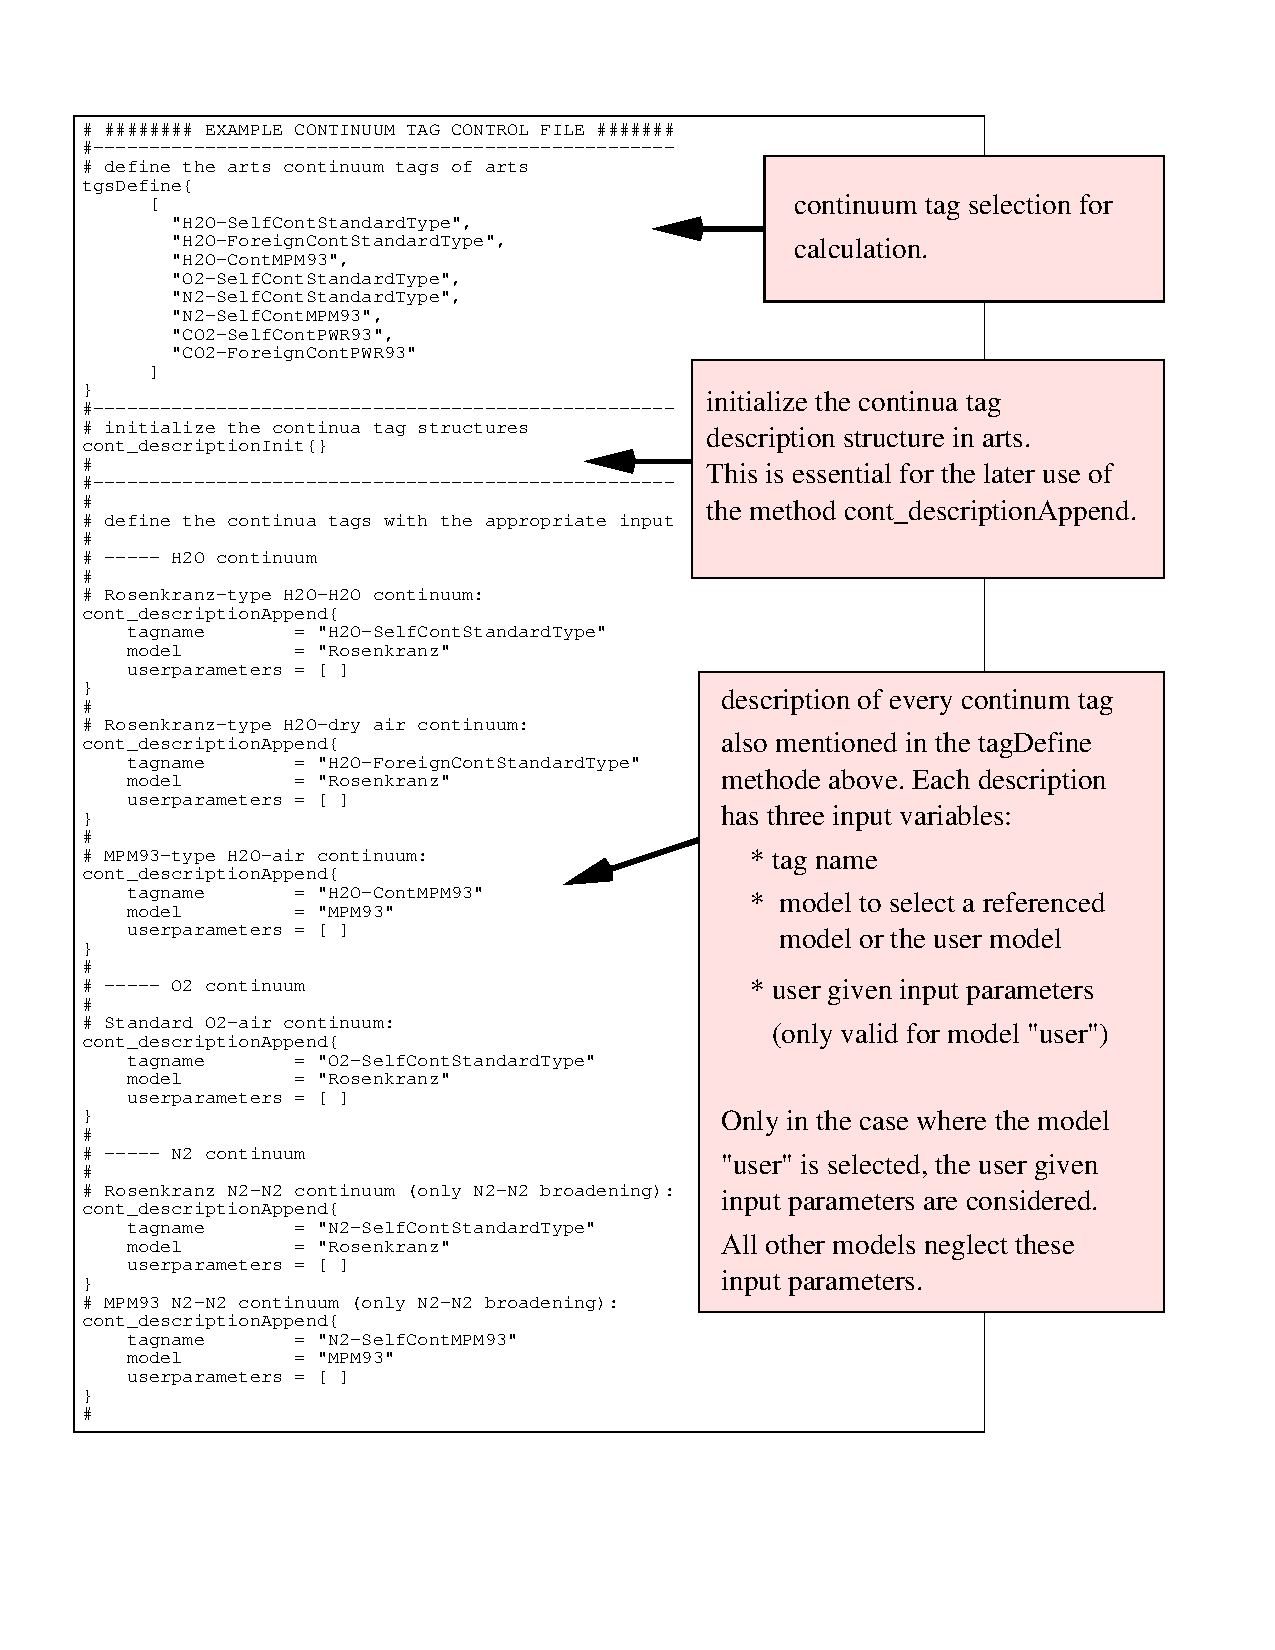
\includegraphics[scale=0.65, angle=0]{cont_description_page1}
\end{flushleft}
\begin{flushleft}
 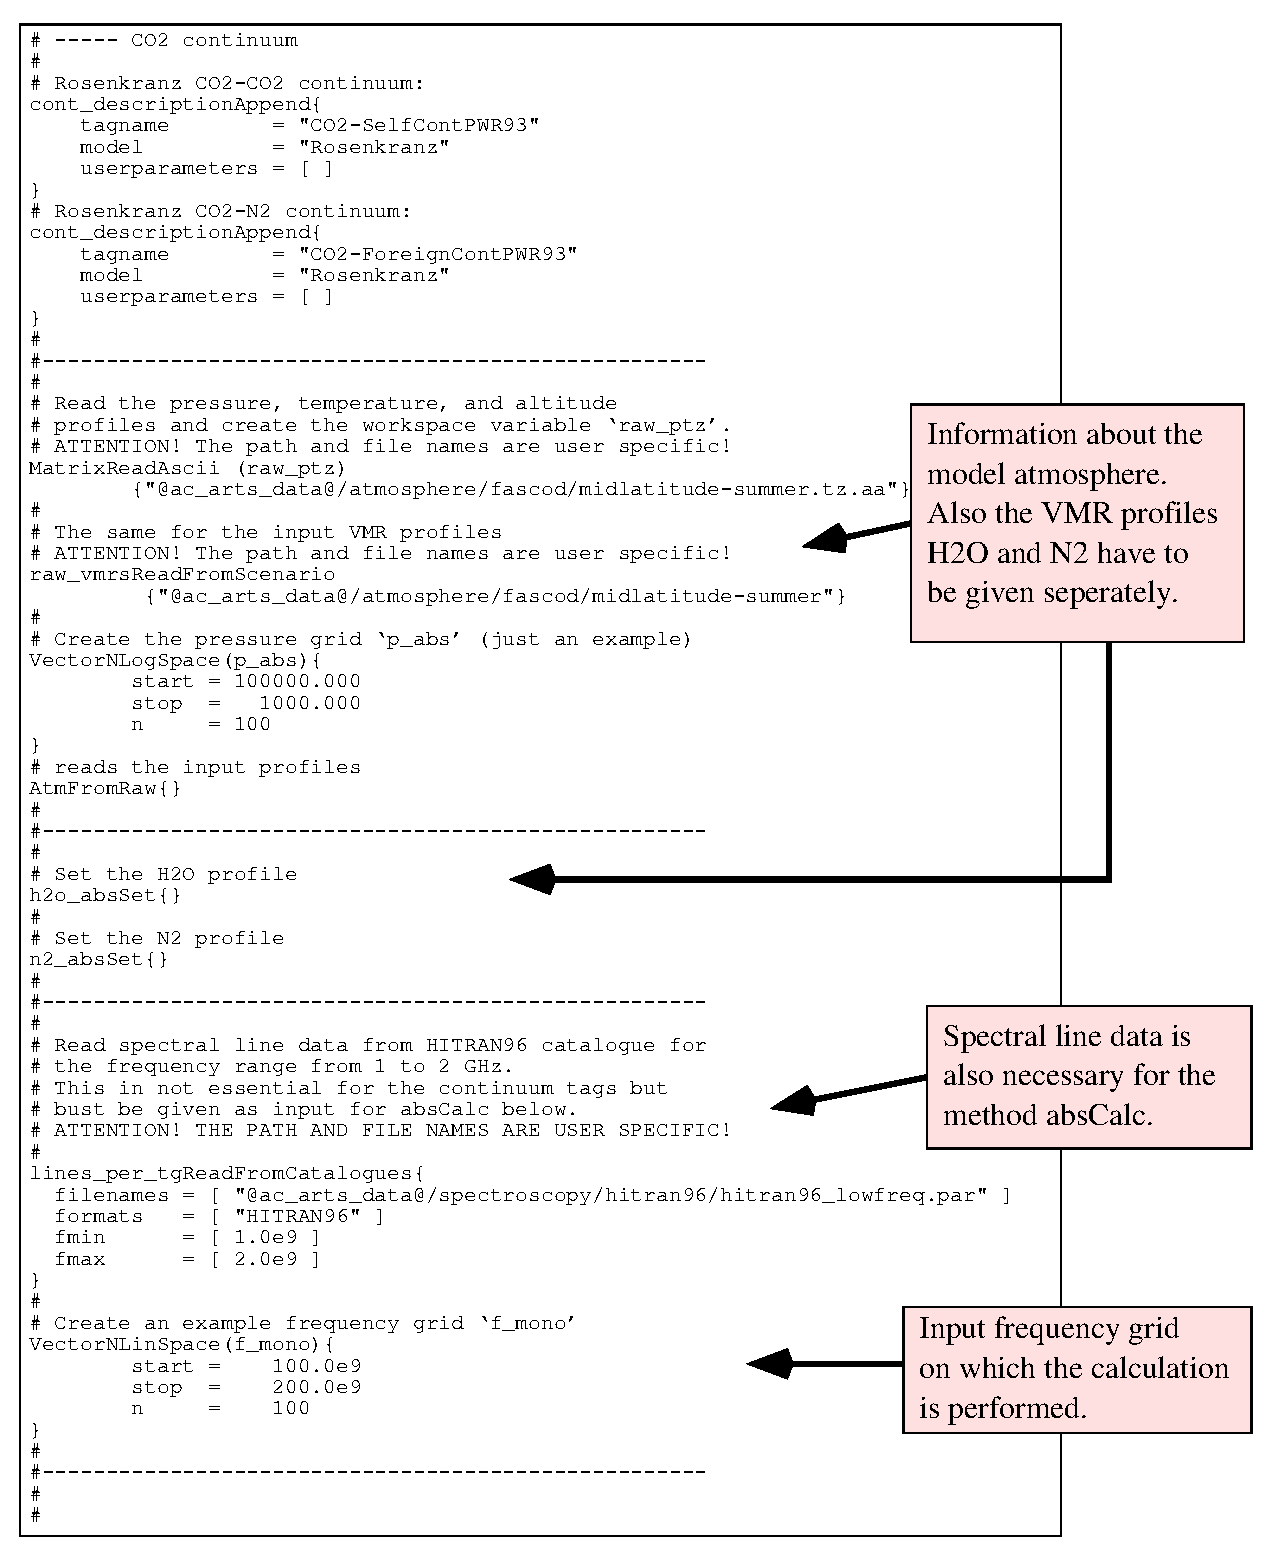
\includegraphics[scale=0.65, angle=0]{cont_description_page2}
\end{flushleft}
\begin{flushleft}
 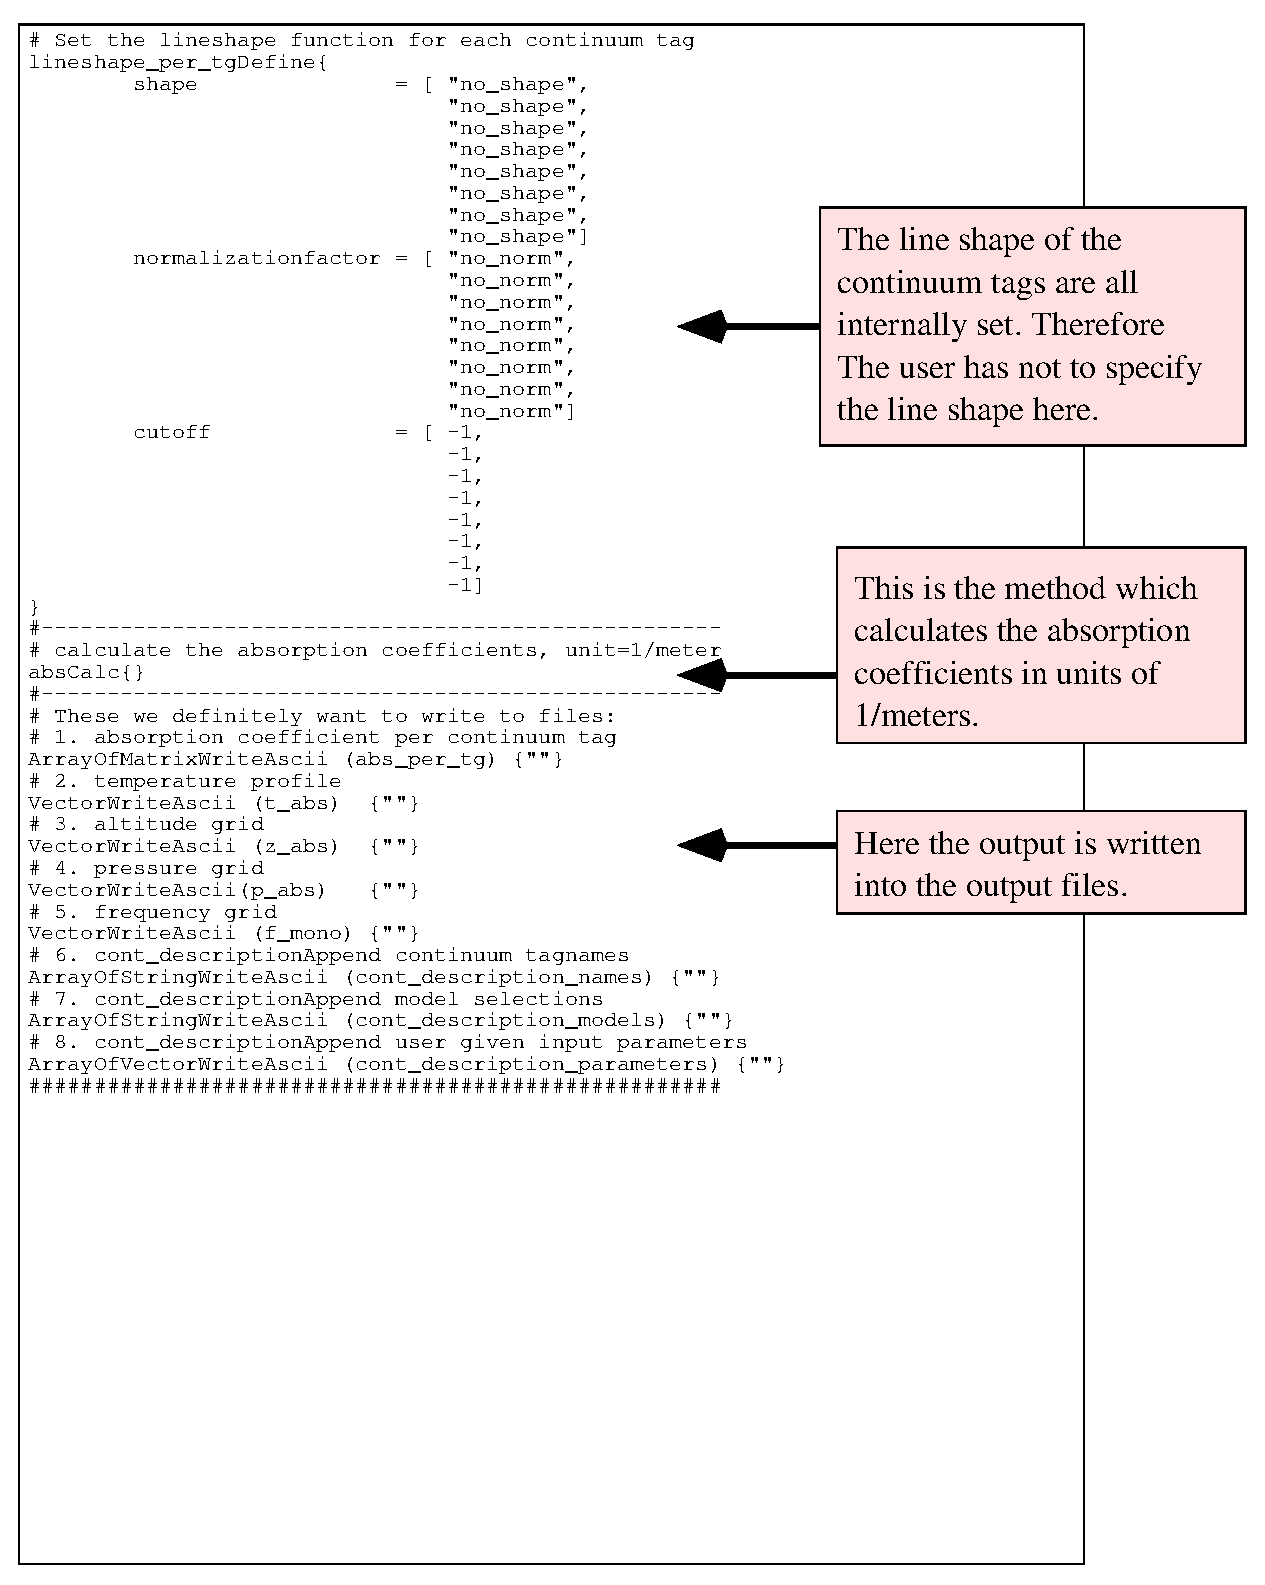
\includegraphics[scale=0.65, angle=0]{cont_description_page3}
\end{flushleft}



% ================================================================================
% The following section is written by Thomas Kuhn, iup Bremen, tkuhn@uni-bremen.de
% ================================================================================



\levelb{Complete Absorption Models}
\label{levelb:CompAbsMod}
% =================================
The MPM absorption model of Liebe and coworkers consists of modules for 
water vapor and oxygen absorption. The Rosenkranz (PWR98) absorption 
model include also $\hzo$ and $\oz$ while the Cruz-Pol et al. (CP98) absorption 
models include absorption due to water vapor. Additionally 
the CP98 model has a strongly reduced parameter set for the $\hzo$-line 
absorption since it is especially intended for the range around the 
22\,GHz water line. The MPM and R98 are valid from the microwave 
up to the submillimeter frequency range (1-1000\,GHz).

Implemented in ARTS are the following modules of the above mentioned models:
%
\begin{center}
\begin{tabular}{ll}
\hline
species & model\\
\hline
$\hzo$ & MPM87, MPM89, MPM93, PWR98, CP98 \\
$\oz$  & MPM93, PWR98 \\
\hline
\end{tabular}
\end{center}




\levelc{Complete Water Vapor Models}
\label{levelc:CompWatVapMod}
% ==================================
In ARTS several complete water vapor absorption models are implemented and 
can easily be used. Implemented models are the versions 
MPM87 \cite{liebeandlayton:87}, MPM89 \cite{liebe:89}, and 
MPM93 \cite{liebeetal:93} of the Liebe Millimeter-wave Propagation Model 
and additionally the models of Cruz-Pol et al. (CP98) \cite{cruzpol:98} 
and P.~W. Rosenkranz (PWR98) \cite{pwr:98}. 
MPM and PWR98 are especially desigend for fast absorption calculations in 
the frequency range of 1-1000\,GHz while the CP98 model is a reduced model 
for a narrow frequency band around the 22\,GHz $\hzo$-line (especially used 
by ground-based radiometers).

The total water vapor absorption ($\alphatot$) is in all the stated models 
described by a line absorption ($\alphal$) term and a continuum absorption 
($\alphac$) term: 
\begin{equation}
  \label{eq:h2o:totabs}
  \alphatot = \alphal + \alphac
\end{equation}
The main differences between the different models is the line shape used for 
$\alphal$ and the formulation of $\alphac$.

It has to be emphasized that, $\alphal$ and $\alphac$ of different
models are not necessarily compatible and should therefore not be 
interchanged between different models.


\leveld{MPM87 Water Vapor Absorption Model}
\label{leveld:mpm87}
%------------------------------------------
This version, which is described in \cite{liebeandlayton:87} and 
follows the general line of the MPM model to divide the total 
water vapor absorption, $\alphampmotot$, into a spectral line 
term, $\alphampmol$, and a continuum term not attributed to 
spectral lines, $\alphampmoc$:
\begin{equation}
  \label{eq:mpm87_abs}
  \alphampmotot = \alphampmol + \alphampmoc\hspace*{10mm}\mbox{dB/km}
\end{equation}



\levele{Water Vapor Line Absorption:}
\label{levele:mpm87_h2olines}
%-----------------------------------
The MPM87 \cite{liebeandlayton:87} water vapor line catalog consists 
of 30 lines from 22\,GHz up to 988\,GHz. The center frequencies and parameter 
values are listed in Table \ref{tab:mpm87linelist}. To describe the line 
absorption, a set of three parameters ($\bek$ and $\bdk$) per line are used: two 
for the line strength and one for the line width. The total line 
absorption coefficient (in units of dB/km) is the sum over all 
individual line absorption coefficients\footnote{The factor 
  $0.1820 \cdot 10^{6}$ is equal to $(4\,\pi/c)\cdot 10\log{(e)}$
  (the term $(4\,\pi/c)$ comes from the definition of the absorption
  coefficient in terms of the dielectric constant and the term 
  $10\,\log{(e)}$ is due to the definition of the Decibel.) The
  velocity of light is defined as $c=2.9979\cdot 10^{-4}$\,km\,GHz. 
  The factor $10^{6}$ is incorporated into the line strength and 
  does therefore not appear in the pre-factor.}:
\begin{equation}
  \label{eq:mpm87:absline}
  \alphampmol = 0.1820 \cdot \nuk \cdot \phzo \cdot 
  \sum_{k}{\inten \cdot \shape}\hspace*{10mm}\mbox{dB/km}
\end{equation}
where $\inten$ is the line intensity described by the parameterization
\begin{equation}
  \label{eq:mpm87:strength}
  \inten = \bek \cdot \phzo \cdot \Theta^{3.5} 
           \cdot \exp{(\bzk \cdot [1-\Theta])}\hspace*{10mm}\mbox{kHz}
\end{equation}
with $\nuk$ as the line center frequency, $\phzo$ the water
vapor partial pressure and $\Theta = 300\,\mbox{K}/T$.\\
The line shape function, $\shape$, in Eq.~(\ref{eq:mpm87:absline}) 
is the standard Van~Vleck-Weisskopf (VVW) function, given by:
\begin{eqnarray}
% Van Vleck-Weisskopf function
  \label{eq:mpm87:VVW}
  \shape & = & \left(\frac{\nu}{\nuk}\right) \cdot 
               \left[\frac{\gamk}{(\nu - \nuk)^2 + \gamk^2} + 
                     \frac{\gamk}{(\nu + \nuk)^2 + \gamk^2}\right]\\
\end{eqnarray}
The pressure broadened line width, $\gamk$, is calculated with the 
single parameter $\bdk$ in the following way:
\begin{equation}
  \label{eq:mpm87:gamma}
  \gamk = \bdk \cdot 
          (4.80 \cdot \phzo \cdot \Theta^{1.1} + \pda \cdot
          \Theta^{0.6})\hspace*{10mm}\mbox{GHz}
\end{equation}
where $\pda$ is the partial pressure of dry air ($\pda=\ptot-\phzo$). 
The parameterizations of $\inten$ and $\gamk$ are already in use for the 
early version of MPM81 \cite{liebe:81}.
%
\begin{longtable}{rrrrr}
 K & K & K & K & K \kill
%
% --------------------- only begin of table ------------------------------
 \hline
       & $\nu_k$ & $\bek$   & $\bzk$ & $\bdk$  \\
% //      [GHz]    [kHz/kPa]   [1]     [GHz/kPa]
 $k$   & {\rm [GHz]}  & {[$\frac{\rm kHz}{\rm kPa}$]} & {\rm [1]} & 
 {[$\frac{\rm GHz}{\rm kPa}$]}\\
 \hline
 \endfirsthead
% --------------------- every page begin of table ------------------------
 \hline
  $k$  & $\nu_k$ & $\bek$ & $\bzk$ & $\bdk$ \\
 \hline
 \endhead
% --------------------- every page end of table ------------------------
 K & K & K & K & K \kill
 \hline
 \caption[]{(continued)}\\
 \endfoot
% --------------------- only end of table ------------------------------
 K & K & K & K & K \kill 
 \hline
 \caption{List of H$_2$O spectral lines and their spectroscopic 
   parameters (H$_2$O-air mixture) for the MPM87 model \cite{liebeandlayton:87}.}
 \label{tab:mpm87linelist}
 \endlastfoot
% --------------------- body of table  ----------------------------------  
% //         0           1           2       3      
% //         f0          b1          b2      b3     
% //        [GHz]       [kHz/kPa]   [1]    [GHz/kPa]
%  const Numeric mpm87[30][4] = { 
1     &    22.235080&    0.1090&  2.143&   27.84$\cdot$ 10$^{-3}$\\
2     &    67.813960&    0.0011&  8.730&   27.60$\cdot$ 10$^{-3}$\\
3     &   119.995940&    0.0007&  8.347&   27.00$\cdot$ 10$^{-3}$\\
4     &   183.310117&    2.3000&  0.653&   31.64$\cdot$ 10$^{-3}$\\
5     &   321.225644&    0.0464&  6.156&   21.40$\cdot$ 10$^{-3}$\\
6     &   325.152919&    1.5400&  1.515&   29.70$\cdot$ 10$^{-3}$\\
7     &   336.187000&    0.0010&  9.802&   26.50$\cdot$ 10$^{-3}$\\
8     &   380.197372&   11.9000&  1.018&   30.36$\cdot$ 10$^{-3}$\\
9     &   390.134508&    0.0044&  7.318&   19.00$\cdot$ 10$^{-3}$\\
10    &   437.346667&    0.0637&  5.015&   13.70$\cdot$ 10$^{-3}$\\
11    &   439.150812&    0.9210&  3.561&   16.40$\cdot$ 10$^{-3}$\\
12    &   443.018295&    0.1940&  5.015&   14.40$\cdot$ 10$^{-3}$\\
13    &   448.001075&   10.6000&  1.370&   23.80$\cdot$ 10$^{-3}$\\
14    &   470.888947&    0.3300&  3.561&   18.20$\cdot$ 10$^{-3}$\\
15    &   474.689127&    1.2800&  2.342&   19.80$\cdot$ 10$^{-3}$\\
16    &   488.491133&    0.2530&  2.814&   24.90$\cdot$ 10$^{-3}$\\
17    &   503.568532&    0.0374&  6.693&   11.50$\cdot$ 10$^{-3}$\\
18    &   504.482692&    0.0125&  6.693&   11.90$\cdot$ 10$^{-3}$\\
19    &   556.936002&  510.0000&  0.114&   30.00$\cdot$ 10$^{-3}$\\
20    &   620.700807&    5.0900&  2.150&   22.30$\cdot$ 10$^{-3}$\\
21    &   658.006500&    0.2740&  7.767&   30.00$\cdot$ 10$^{-3}$\\
22    &   752.033227&  250.0000&  0.336&   28.60$\cdot$ 10$^{-3}$\\
23    &   841.073593&    0.0130&  8.113&   14.10$\cdot$ 10$^{-3}$\\
24    &   859.865000&    0.1330&  7.989&   28.60$\cdot$ 10$^{-3}$\\
25    &   899.407000&    0.0550&  7.845&   28.60$\cdot$ 10$^{-3}$\\
26    &   902.555000&    0.0380&  8.360&   26.40$\cdot$ 10$^{-3}$\\
27    &   906.205524&    0.1830&  5.039&   23.40$\cdot$ 10$^{-3}$\\
28    &   916.171582&    8.5600&  1.369&   25.30$\cdot$ 10$^{-3}$\\
29    &   970.315022&    9.1600&  1.842&   24.00$\cdot$ 10$^{-3}$\\
30    &   987.926764&  138.0000&  0.178&   28.60$\cdot$ 10$^{-3}$\\
\hline
% -----------------------------------------------------------------------  
\end{longtable}


\levele{Water Vapor Continuum Absorption:}
\label{levele:mpm87_h2ocont}
%----------------------------------------
The water vapor continuum absorption coefficient in MPM87, $\alphampmoc$, 
is determined from laboratory measurements at 137.8\,GHz by Liebe 
and Layton covering the following parameter range:\\
\begin{tabular}{lr}
temperature          & 282-316\,K\\
relative humidity    & 0-95\,\%\\
dry air pressure     & 0 - 160\,kPa\\ 
\end{tabular}\\
The mathematical expression of $\alphampmoc$ is derived from the far wing 
approximation of the line absorption and is expressed as follows
\begin{equation} 
  \label{eq:mpm87:cont}
  \alphampmoc = \nu^2 \cdot \phzo \cdot 
                (\cso \cdot \phzo \cdot \Theta^{\xs} + 
                 \cdo \cdot \pda  \cdot \Theta^{\xf}),
\end{equation}
with the continuum parameter set $\cso$, $\cdo$, $\xs$, and $\xf$. 
The determined values of the continuum parameters are:

\begin{description}
\item{$\cso$}   =  6.496\,$\cdot$\,10$^{-6}$~~(dB/km)~/~(hPa$\cdot$GHz)$^2$
\item{$\xs$}    = 10.5
\item{$\cdo$}   =  0.206\,$\cdot$\,10$^{-6}$~~(dB/km)~/~(hPa$\cdot$GHz)$^2$
\item{$\xd$}    =  3.0
\end{description}




\leveld{MPM89 Water Vapor Absorption Model}
\label{leveld:mpm89}
%------------------------------------------
%
MPM89 is described in \cite{liebe:89} and follows the general line 
of the MPM model to devide the total water vapor absorption, 
$\alphampmmtot$, into a spectral line term, $\alphampmml$, and a continuum 
term not attributed to spectral lines, $\alphampmmc$:
\begin{equation}
  \label{eq:mpm89_abs}
  \alphampmmtot = \alphampmml + \alphampmmc\hspace*{10mm}\mbox{dB/km}
\end{equation}
All the absorption coefficients are calculated in units of \mbox{dB/km}.


\levele{Water Vapor Line Absorption:}
\label{levele:mpm89_h2olines}
%-----------------------------------
The MPM89 water vapor line catalog consists of the same 30 lines 
like MPM87 from 22\,GHz up to 988\,GHz. The center frequencies and parameter 
values are listed in Table \ref{tab:mpm89linelist}. To describe the line 
absorption, a set of six parameters ($\bek$ and $\bsk$) per line are used: two 
for the line strength and four for the line width. The total line 
absorption coefficient (in units of dB/km) is the sum over all
individual line absorption coefficients\footnote{see footnote for
  MPM97 line absorption}:
\begin{equation}
  \label{eq:mpm89:absline}
  \alphampmml = 0.1820 \cdot \nuk \cdot \phzo \cdot 
  \sum_{k}{\inten \cdot \shape}\hspace*{10mm}\mbox{dB/km}
\end{equation}
where $\inten$ is the line intensity described by the parameterization
\begin{equation}
  \label{eq:mpm89:strength}
  \inten = \bek \cdot \phzo \cdot \Theta^{3.5} 
           \cdot \exp{(\bzk \cdot [1-\Theta])}\hspace*{10mm}\mbox{kHz}
\end{equation}
whit $\nuk$ as the line center frequency, $\phzo$ the water
vapor partial pressure and $\Theta = 300\,\mbox{K}/T$.\\
The line shape function, $\shape$, in Eq.~(\ref{eq:mpm89:absline}) 
is the standard Van Vleck-Weisskopf (VVW) function, given by 
\begin{eqnarray}
% Van Vleck-Weisskopf function
  \label{eq:mpm89:VVW}
  \shape & = & \left(\frac{\nu}{\nuk}\right) \cdot 
               \left[\frac{\gamk}{(\nu - \nuk)^2 + \gamk^2} + 
                     \frac{\gamk}{(\nu + \nuk)^2 + \gamk^2}\right]
\end{eqnarray}
where the pressure broadened line width, $\gamk$, is calculated as
\begin{equation}
  \label{eq:mpm89:gamma}
  \gamk = \bdk \cdot 
         (\bfk \cdot \phzo \cdot \Theta^{\bsk} + 
                     \pda  \cdot \Theta^{\bvk})
        \cdot 10^{-3}\hspace*{10mm}\mbox{GHz}
\end{equation}
with $\pda=\ptot-\phzo$ as the dry air partial pressure. 
The only difference between MPM87 and MPM89 with respect to the line 
absorption is the parameterization of the pressure broadened line
width, $\gamk$, which is calculated with the four parameters $\bdk$ to
$\bsk$ in the case of MPM89 whereas in MPM87 a single parameter
($\bdk$) is used (see Eq.~(\ref{eq:mpm87:gamma})).
%
\begin{longtable}{rrrrrrrr}
 K & K & K & K & K & K & K & K \kill
%
% --------------------- only begin of table ------------------------------
 \hline
    & $\nu_k$ & $\bek$ & $\bzk$ & $\bdk$ & $\bvk$ & $\bfk$ & $\bsk$ \\
%    [GHz]     [kHz/kPa]   [1]   [MHz/kPa]  [1]    [1]    [1]
 $k$& {\rm [GHz]}  & {[$\frac{\rm kHz}{\rm kPa}$]} & {\rm [1]} & 
 {[$\frac{\rm MHz}{\rm kPa}$]} & {\rm [1]} & {\rm [1]} & {\rm [1]} \\
 \hline
 \endfirsthead
% --------------------- every page begin of table ------------------------
 \hline
  $k$  & $\nu_k$ & $\bek$ & $\bzk$ & $\bdk$ & $\bvk$ & $\bfk$ & $\bsk$ \\
 \hline
 \endhead
% --------------------- every page end of table ------------------------
 K & K & K & K & K & K & K & K \kill
 \hline
 \caption[]{(continued)}\\
 \endfoot
% --------------------- only end of table ------------------------------
 K & K & K & K & K & K & K & K \kill
 \hline
 \caption{List of H$_2$O spectral lines and their spectroscopic 
   parameters (H$_2$O-air mixture) for the MPM89 model \cite{liebe:89}.}
 \label{tab:mpm89linelist}
 \endlastfoot
% --------------------- body of table  ----------------------------------  
%            0           1        2       3        4      5      6
%            f0          b1       b2      b3       b4     b5     b6
%          [GHz]     [kHz/kPa]   [1]   [MHz/kPa]  [1]    [1]    [1]
%  const Numeric mpm89[30][7] = { 
1    &    22.235080&    0.1090&  2.143&   28.11&   0.69&  4.80&  1.00\\
2    &    67.813960&    0.0011&  8.735&   28.58&   0.69&  4.93&  0.82\\
3    &   119.995940&    0.0007&  8.356&   29.48&   0.70&  4.78&  0.79\\
4    &   183.310074&    2.3000&  0.668&   28.13&   0.64&  5.30&  0.85\\
5    &   321.225644&    0.0464&  6.181&   23.03&   0.67&  4.69&  0.54\\
6    &   325.152919&    1.5400&  1.540&   27.83&   0.68&  4.85&  0.74\\
7    &   336.187000&    0.0010&  9.829&   26.93&   0.69&  4.74&  0.61\\
8    &   380.197372&   11.9000&  1.048&   28.73&   0.69&  5.38&  0.84\\
9    &   390.134508&    0.0044&  7.350&   21.52&   0.63&  4.81&  0.55\\
10    &   437.346667&    0.0637&  5.050&   18.45&   0.60&  4.23&  0.48\\
11    &   439.150812&    0.9210&  3.596&   21.00&   0.63&  4.29&  0.52\\
12    &   443.018295&    0.1940&  5.050&   18.60&   0.60&  4.23&  0.50\\
13    &   448.001075&   10.6000&  1.405&   26.32&   0.66&  4.84&  0.67\\
14    &   470.888947&    0.3300&  3.599&   21.52&   0.66&  4.57&  0.65\\
15    &   474.689127&    1.2800&  2.381&   23.55&   0.65&  4.65&  0.64\\
16    &   488.491133&    0.2530&  2.853&   26.02&   0.69&  5.04&  0.72\\
17    &   503.568532&    0.0374&  6.733&   16.12&   0.61&  3.98&  0.43\\
18    &   504.482692&    0.0125&  6.733&   16.12&   0.61&  4.01&  0.45\\
19    &   556.936002&  510.0000&  0.159&   32.10&   0.69&  4.11&  1.00\\
20    &   620.700807&    5.0900&  2.200&   24.38&   0.71&  4.68&  0.68\\
21    &   658.006500&    0.2740&  7.820&   32.10&   0.69&  4.14&  1.00\\
22    &   752.033227&  250.0000&  0.396&   30.60&   0.68&  4.09&  0.84\\
23    &   841.073593&    0.0130&  8.180&   15.90&   0.33&  5.76&  0.45\\
24    &   859.865000&    0.1330&  7.989&   30.60&   0.68&  4.09&  0.84\\
25    &   899.407000&    0.0550&  7.917&   29.85&   0.68&  4.53&  0.90\\
26    &   902.555000&    0.0380&  8.432&   28.65&   0.70&  5.10&  0.95\\
27    &   906.205524&    0.1830&  5.111&   24.08&   0.70&  4.70&  0.53\\
28    &   916.171582&    8.5600&  1.442&   26.70&   0.70&  4.78&  0.78\\
29    &   970.315022&    9.1600&  1.920&   25.50&   0.64&  4.94&  0.67\\
30    &   987.926764&  138.0000&  0.258&   29.85&   0.68&  4.55&  0.90\\
\hline
% -----------------------------------------------------------------------  
\end{longtable}


\levele{Water Vapor Continuum Absorption:}
\label{levele:mpm89_h2ocont}
%----------------------------------------
The MPM89 continuum absorption coefficients in, $\alphampmmc$, 
are identical as those in MPM87 (see Sec. \ref{levele:mpm87_h2ocont} for 
details):
\begin{equation} 
  \label{eq:mpm89:cont}
  \alphampmmc = \nu^2 \cdot \phzo \cdot 
                (\cso \cdot \phzo \cdot \Theta^{\xs} + 
                 \cdo \cdot \pda  \cdot \Theta^{\xf}),
\end{equation}
with
\begin{description}
\item{$\cso$}   =  6.496\,$\cdot$\,10$^{-6}$~~(dB/km)~/~(hPa$\cdot$GHz)$^2$
\item{$\xs$}    = 10.5
\item{$\cdo$}   =  0.206\,$\cdot$\,10$^{-6}$~~(dB/km)~/~(hPa$\cdot$GHz)$^2$
\item{$\xd$}    =  3.0
\end{description}





\leveld{MPM93 Water Vapor Absorption Model}
\label{leveld:mpm93}
%----------------------------------------------
This version, which is described in \cite{liebeetal:93} and 
follows the general line of the MPM model to devide the total 
water vapor absorption, $\alphampmntot$, into a spectral line 
term, $\alphampmnl$, and a continuum term not attributed to 
spectral lines, $\alphampmnc$:
\begin{equation}
  \label{eq:mpm93_abs}
  \alphampmntot = \alphampmnl + \alphampmnc\hspace*{10mm}\mbox{dB/km}
\end{equation}
The continuum absorption is parameterized like a
resonant spectral line of $\hzo$, a so-called pseudo-line. This is a 
fundamental change in the parameterization of the water vapor
continuum in respect to all older versions of MPM, which makes it 
quite complicate to compare the different versions, especially to 
distinguish a self- and foreign broadening term in the continuum.



\levele{Water Vapor Line Absorption:}
\label{levele:mpm93_h2olines}
%-----------------------------------
The water vapor line spectrum of MPM93 \cite{liebeetal:93} 
consists of 34 lines below 1\,THz (four more than in MPM89 and MPM87). 
To describe the MPM93 water vapor line absorption, a set of six parameters 
($\bek$ and $\bdk$) per line are used: two for the line strength and 
four for the line width. The total line absorption coefficient 
(in units of dB/km) is the sum over all individual line absorption 
coefficients\footnote{see footnote for MPM97 line absorption}:
\begin{equation}
  \label{eq:mpm93:absline}
  \alphampmnl = 0.1820 \cdot \nuk \cdot \phzo \cdot 
  \sum_{k}{\inten \cdot \shape}\hspace*{10mm}\mbox{dB/km}
\end{equation}
where $\inten$ is the line intensity described by the parameterization
\begin{equation}
  \label{eq:mpm93:strength}
  \inten = \bek \cdot \phzo \cdot \Theta^{3.5} 
           \cdot \exp{(\bzk \cdot [1-\Theta])}\hspace*{10mm}\mbox{kHz}
\end{equation}
with $\nuk$ as the line center frequency, $\phzo$ the water
vapor partial pressure and $\Theta = 300\,\mbox{K}/T$.\\
The line shape function, $\shape$, in Eq.~(\ref{eq:mpm87:absline}) 
is the standard Van~Vleck-Weisskopf (VVW) function, given by:
\begin{eqnarray}
% Van Vleck-Weisskopf function
  \label{eq:mpm93:VVW}
  \shape & = & \left(\frac{\nu}{\nuk}\right) \cdot 
               \left[\frac{\gamk}{(\nu - \nuk)^2 + \gamk^2} + 
                     \frac{\gamk}{(\nu + \nuk)^2 + \gamk^2}\right]\\
\end{eqnarray}
The pressure broadened line width, $\gamk$, is calculated with the 
single parameter $\bdk$ in the following way:
\begin{equation}
  \label{eq:mpm93:gamma}
  \gamk = \bdk \cdot 
          (4.80 \cdot \phzo \cdot \Theta^{1.1} + \pda \cdot
          \Theta^{0.6})\hspace*{10mm}\mbox{GHz}
\end{equation}
where $\pda$ is the partial pressure of dry air ($\pda=\ptot-\phzo$). 

The parameterizations of $\inten$ was already in use for the early 
version of MPM81 \cite{liebe:81}. The expression for $\gamk$ is the
same as in MPM89. The main difference between MPM93 and MPM89 
concerning the water vapor line absorption is the updated line catalog.
%
%
%\begin{landscape}
%\setlength{\LTcapwidth}{200mm} % with of the caption in longtable
\begin{longtable}{rrrrrrrr}
 K & K & K & K & K & K & K & K \kill
%
% --------------------- only begin of table ------------------------------
 \hline
       & $\nu_k$ & $\bek$ & $\bzk$ & $\bdk$ & $\bvk$ & $\bfk$ & $\bsk$ \\
 $k$   & {\rm [GHz]}  & {[$\frac{\rm kHz}{\rm hPa}$]} & {\rm [1]} & 
 {[$\frac{\rm MHz}{\rm hPa}$]} & {\rm [1]} & {\rm [1]} & {\rm [1]} \\
 \hline
 \endfirsthead
% --------------------- every page begin of table ------------------------
 \hline
    & $\nu_k$ & $\bek$ & $\bzk$ & $\bdk$ & $\bvk$ & $\bfk$ & $\bsk$ \\
 \hline
 \endhead
% --------------------- every page end of table ------------------------
 K & K & K & K & K & K & K & K \kill
 \hline
 \caption[]{(continued)}\\
 \endfoot
% --------------------- only end of table ------------------------------
 K & K & K & K & K & K & K & K \kill
 \hline
 \caption{List of used H$_2$O spectral lines and their spectroscopic 
   coefficients of H$_2$O in air for the MPM93 model \citep{liebeetal:93}. 
   The last separated line is the unphysical pseudo-line used in MPM93. 
   The lines which are marked with a "$^+$" were not in the MPM87/MPM89 
   line catalog.}
 \label{tab:mpm93linelist}
 \endlastfoot
% --------------------- body of table  ----------------------------------  
1      & 22.235080  & 0.01130 & 2.143 & 2.811 & 4.80 & 0.69 & 1.00 \\
2      & 67.803960  & 0.00012 & 8.735 & 2.858 & 4.93 & 0.69 & 0.82 \\
3      & 119.995940 & 0.00008 & 8.356 & 2.948 & 4.78 & 0.70 & 0.79 \\
4      & 183.310091 & 0.24200 & 0.668 & 3.050 & 5.30 & 0.64 & 0.85 \\
5      & 321.225644 & 0.00483 & 6.181 & 2.303 & 4.69 & 0.67 & 0.54 \\ 
6      & 325.152919 & 0.14990 & 1.540 & 2.783 & 4.85 & 0.68 & 0.74 \\
7      & 336.222601 & 0.00011 & 9.829 & 2.693 & 4.74 & 0.69 & 0.61 \\ 
8      & 380.197372 & 1.15200 & 1.048 & 2.873 & 5.38 & 0.54 & 0.89 \\
9      & 390.134508 & 0.00046 & 7.350 & 2.152 & 4.81 & 0.63 & 0.55 \\
10     & 437.346667 & 0.00650 & 5.050 & 1.845 & 4.23 & 0.60 & 0.48 \\
11     & 439.150812 & 0.09218 & 3.596 & 2.100 & 4.29 & 0.63 & 0.52 \\
12     & 443.018295 & 0.01976 & 5.050 & 1.860 & 4.23 & 0.60 & 0.50 \\
13     & 448.001075 & 1.03200 & 1.405 & 2.632 & 4.84 & 0.66 & 0.67 \\
14     & 470.888947 & 0.03297 & 3.599 & 2.152 & 4.57 & 0.66 & 0.65 \\
15     & 474.689127 & 0.12620 & 2.381 & 2.355 & 4.65 & 0.65 & 0.64 \\
16     & 488.491133 & 0.02520 & 2.853 & 2.602 & 5.04 & 0.69 & 0.72 \\
17     & 503.568532 & 0.00390 & 6.733 & 1.612 & 3.98 & 0.61 & 0.43 \\
18     & 504.482692 & 0.00130 & 6.733 & 1.612 & 4.01 & 0.61 & 0.45 \\
19$^+$ & 547.676440 & 0.97010 & 0.114 & 2.600 & 4.50 & 0.70 & 1.00 \\
20$^+$ & 552.020960 & 1.47700 & 0.114 & 2.600 & 4.50 & 0.70 & 1.00 \\
21     & 556.936002 & 48.74000& 0.159 & 3.210 & 4.11 & 0.69 & 1.00 \\
22     & 620.700807 & 0.50120 & 2.200 & 2.438 & 4.68 & 0.71 & 0.68 \\
23$^+$ & 645.866155 & 0.00713 & 8.580 & 1.800 & 4.00 & 0.60 & 0.50 \\
24     & 658.005280 & 0.03022 & 7.820 & 3.210 & 4.14 & 0.69 & 1.00 \\
25     & 752.033227 & 23.96000& 0.396 & 3.060 & 4.09 & 0.68 & 0.84 \\
26     & 841.053973 & 0.00140 & 8.180 & 1.590 & 5.76 & 0.33 & 0.45 \\
27     & 859.962313 & 0.01472 & 7.989 & 3.060 & 4.09 & 0.68 & 0.84 \\
28     & 899.306675 & 0.00605 & 7.917 & 2.985 & 4.53 & 0.68 & 0.90 \\
29     & 902.616173 & 0.00426 & 8.432 & 2.865 & 5.10 & 0.70 & 0.95 \\
30     & 906.207325 & 0.01876 & 5.111 & 2.408 & 4.70 & 0.70 & 0.53 \\
31     & 916.171582 & 0.83400 & 1.442 & 2.670 & 4.78 & 0.70 & 0.78 \\
32$^+$ & 923.118427 & 0.00869 & 10.220& 2.900 & 5.00 & 0.70 & 0.80 \\
33     & 970.315022 & 0.89720 & 1.920 & 2.550 & 4.94 & 0.64 & 0.67 \\
34     & 987.926764 & 13.21000& 0.258 & 2.985 & 4.55 & 0.68 & 0.90 \\
\hline
 & $\nu^*$ & $\beks$ & $\bzks$ & $\bdks$ & $\bvks$ & $\bfks$ & $\bsks$\\
 & {\rm [GHz]}  & {[$\frac{\rm kHz}{\rm hPa}$]} & {\rm [1]} & 
 {[$\frac{\rm MHz}{\rm hPa}$]} & {\rm [1]} & {\rm [1]} & {\rm [1]} \\
\hline
 & 1780.000000 & 2230.00000 & 0.952 & 17.620 & 30.50 & 2.00 & 5.00 \\
% -----------------------------------------------------------------------  
\end{longtable}
%\setlength{\LTcapwidth}{0.8\textwidth}
%\end{landscape}



\levele{The MPM93 Continuum Parameterization:}
\label{levele:mpm93:h2ocont}
%-----------------------------------------------
In the MPM93 version the water vapor continuum is parameterized as an
ordinary spectral line (Eqs. (\ref{eq:mpm93:strength}, 
\ref{eq:mpm93:VVW})). The parameters of this continuum "pseudo-line" 
($\nu^*$, $\beks$, $\bzks$, $\bdks$, $\bvks$, $\bfks$, $\bsks$) 
are given in Table \ref{tab:mpm93linelist}. More details about 
this continuum parameterization and its microwave approximation can be 
found in Section \ref{leveld:h2o_Cont} of this guide.




\leveld{CP98 Water Vapor Absorption Model}
\label{leveld:cp98}
%---------------------------------------------

\levele{Line Absorption}
\label{levele:cp98_h2oline}
%--------------------------
component \citep{cruzpol:98} for the water vapor line absorption 
is based on MPM87 with the main difference that the 
line catalog consists of only a single line at $\nu_{\rm o}=$\,22\,GHz. 
The contributions from the other lines is put into the water vapor 
continuum module. The line absorption is therefore very quickly 
calculated (in units of Np/km) according to the formula
\begin{eqnarray}
  \label{eq:cp98:lineabs}
  \alphacpl &=& 0.0419 \cdot \intencp \cdot \shape \\
  \mbox{with} & & \nonumber\\
  \label{eq:cp98:inten}
  \intencp    &=& 0.0109 \cdot C_L \cdot \phzo \cdot \nuo \cdot \Theta^{3.5} 
             \cdot \exp{(2.143\cdot[1-\Theta])}\nonumber\\
%
  \label{eq:cp98:width}
  \gamma &=& 0.002784 \cdot C_W \cdot (\pda \cdot \Theta^{0.6}+ 
             4.8 \cdot \phzo \cdot \Theta^{1.1}) \nonumber\\
\end{eqnarray}
where $\phzo$ and $\pda$ are the partial pressure of water vapor and dry
air in units of hPa, respectively and the Van Vleck-Weisskopf line
shape, $\shape$. The numbers correspond to the line
parameters form MPM87 for this special line and the factors  
$C_L$ and $C_W$ are adjustable scaling factors to match the model with the
measurements. Setting the scaling factors to $C_L$=1.00 and $C_W$=1.00 
leads to the same results as for MPM87. According to the parameter 
estimation of Cruz--Pol et al. best agreement between 
data and model is obtained with $C_L=$\,1.0639$\pm$0.016 and 
$C_W=$\,1.0658$\pm$0.0096. The correlation between these two scaling 
factors was found to be negligible, as can be seen from 
Table \ref{tab:cp_orr}.

\begin{table}[!htb]
\begin{center}
\begin{tabular}{lllll}
\hline
            & $C_L$ & $C_W$ & $C_C$ & $C_X$ \\
\hline
value       & 1.0639 & 1.0658 & 1.2369 & 1.0739\\
std. dev.   & 0.016  & 0.0096 & 0.155  & 0.252\\
\hline
correlation & &&&\\
$C_L$       & 1      & -0.085 & 0.045  & -0.048\\
$C_W$       & -0.085 & 1      & -0.513 &  0.485\\
$C_C$       & 0.045  & -0.513 & 1      & -0.989\\
$C_X$       & -0.048 & 0.485  & -0.989 & 1\\
\hline
\end{tabular}
\end{center}
\caption{Scaling parameter values with standard deviation and 
  correlation coefficients according to \citep{cruzpol:98}.
  The scaling parameters are $C_L$:22\,GHz line strength, 
  $C_W$:22\,GHz line width , $C_C$:$\hzo$-continuum, and 
  $C_X$:$\oz$-absorption. $C_X$ scales the entire oxygen absorption, 
  the continuum as well as the line absorption. The Cruz-Pol et al.
  model uses the \cite{pwr:93} oxygen absorption model.}
\label{tab:cp_orr}
\end{table}

The main reason why the Cruz-Pol model (CP98) considers only one line
lies in the fact that CP98 is especially designed for the data analysis
in the 20-31.4\,GHz region. The determination of the scaling factors was 
performed with ground based radiometer data in the frequency range of
from different locations\footnote{The data were recorded at San Diego, 
California (11. December 1991) and West Palm Beach, Florida 
(8.-21. March 1992)} in the USA.


\levele{Water Vapor Continuum Absorption:}
\label{levele:cp98_h2ocont}
%-----------------------------------------
The CP98 model uses the same water vapor continuum 
parameterization as MPM87, just scaled with an empirical 
factor, $CC$, determined from the above mentioned data:
\begin{equation}
 \label{eq:cp98_cont_scaling}
 \alphacpc = C_C \cdot \alphampmoc 
\end{equation}
The scaling factor $C_C$, as given in Table \ref{tab:cp_orr}, 
gives a 23.69\,\% increased continuum absorption compared 
with MPM87 (see Table \ref{tab:wvcontparam} for a comparison of the 
parameter values). But one has to keep in mind that $C_C$ has a 
high correlation with the scaling factor of the oxygen 
absorption, $C_X$, since these two components could not 
be completely distinguished in the data. Therefore the 
value of 23.69\,\% has a standard deviation of 15.5\,\% 
and is not so reliable than $C_L$ and $C_W$.





\leveld{PWR98 Water Vapor Absorption Model}
\label{leveld:pwr98_h2o}
%------------------------------------------
The water vapor continuum formulation of \citet{pwr:98} is a re-investigation 
of the existing models MPM87/MPM89, MPM93, and CKD\_2.1 especially for 
the frequency region below 1-1000\,GHz. in the context of the available
laboratory and atmospheric data \citep{abaueretal:89, abaueretal:93, 
abaueretal:95, beckerautler:46, englishetal:94, godonetal:92,
liebe:84, liebeandlayton:87, westwateretal:90}.

Rosenkranz adopted the structure of MPM89 for his improved model (R98). 
However, some important differences exist compared with MPM89:
\begin{itemize}
\item the water vapor line catalogs are different 
\item the R98 uses the Van~Vleck--Weisskopf line shape function with 
      cutoff and MPM89 without cutoff
\end{itemize}


\levele{Water Vapor Line Absorption:}
\label{levele:pwr98_h2oline}
%------------------------------------
The local line absorption is defined as 
\begin{eqnarray} 
 \label{eq:pwr98absline}
 \alphapwrl &=& N_{H_2O} \cdot \sum_k \inten \cdot \shapec \nonumber\\
            &=& N_{H_2O} \cdot \sum_k \inten \cdot 
                \left (\displaystyle{\frac{\nu}{\nuk}}\right )^2  \cdot 
                \left [\shapefp + \shapefm \right]~~\mbox{Np/km}
\end{eqnarray}
where $N_{H_2O}$ is the number density of water molecules, $\nu$ the
frequency and $S$ the line intensity, calculated from the HITRAN92
data base \citet{rothman:92}. Considered for this re-investigation are 
15 lines with a frequency lower than 1\,THz as listed in 
Table \ref{tab:pwr98linelist}.

The line shape function $\shapec$ has a cutoff frequency, $\nucut$,
and a baseline subtraction similar to the CKD model \cite{clough:89}.
The introduction of a cutoff frequency has two advantages: (1) the
cutoff avoids applying the line shape to distant frequencies where the 
line form is theoretically not well understood and (2) the cutoff also
establishes a limit to the summation in Eq.~(\ref{eq:pwr98absline}) where lines
far away from the cutoff limit do not contribute to the sum.  
The Rosenkranz formulation uses the same value for
the cutoff frequency as the CKD model:
\begin{equation} 
 \label{cutoff}
 \nucut = 750\mbox{ GHz}
\end{equation}
%
The explicit mathematical form of the line shape function is defined 
in such a way that in the limit $\nucut \rightarrow \infty$ the 
combination of Eq.~(\ref{eq:pwr98absline}) with the line shape function would 
be equivalent to a Van Vleck--Weisskopf \citep{vanvleck:45} line shape: 
\begin{equation}
 \label{eq:pwr98lineshape}
 \hspace*{-8mm}\shapefpm = 
   \left \{ \begin{array}{r@{\quad:\quad}l} 
   \displaystyle{\frac{\gamk}{\pi}} 
   \left \{ \displaystyle{\frac{1}{(\nu \mp \nuk)^2 + \gamk^2}} - 
   \displaystyle{\frac{1}{\nucut^2 + \gamk^2}} \right \}
   & |\nu \pm \nuk| < \nucut \\ 
   0 & |\nu \pm \nuk| \geq \nucut
                       \end{array} \right.
\end{equation}
$\nuk$ is the line center frequency and $\gamk$ the line
half width, which is calculated according to 
\begin{equation}
 \label{eq:pwr98gamma}
 \gamk = \ws \cdot \phzo \cdot \Theta^{\xs} + 
         \wf \cdot \pda  \cdot \Theta^{\xf}\hspace*{10mm}\mbox{GHz}
\end{equation}
with $\phzo$ and $\pda$ as the partial pressure of water vapor and of 
dry air, respectively. The line depending parameters $\ws$, $\xs$, 
$\wf$, and $\xf$ are listed in Table \ref{tab:pwr98linelist} and the 
dimensionless parameter $\Theta$ is defined as $\Theta$\,=\,300\,K/$T$.

Because of the structural similarity to MPM89, the line broadening 
parameters differ only in minor respects from the values used therein 
(only the parameters $x_{\rm s,1}$, $w_{\rm f,2}$ and $\rm w_{\rm s,2}$ 
are significantly different).
%
\begin{table}[!htb]
\begin{center}
\begin{tabular}{rrrrrr}
 \hline
 index &  $\nuk$      & $\wf$     & $\xf$ & $\ws$     & $\xs$ \\
   k   &  [GHz]       & [GHz/kPa] & [1]   & [GHz/kPa] & [1] \\ 
 \hline
   1   &   22.2351    & 0.00281   & 0.69  & 0.01349   &  0.61 \\
   2   &  183.3101    & 0.00281   & 0.64  & 0.01491   &  0.85 \\
   3   &  321.2256    & 0.00230   & 0.67  & 0.01080   &  0.54 \\
  4    &  325.1529    & 0.00278   & 0.68  & 0.01350   &  0.74 \\
  5    &  380.1974    & 0.00287   & 0.54  & 0.01541   &  0.89 \\
  6    &  439.1508    & 0.00210   & 0.63  & 0.00900   &  0.52 \\
  7    &  443.0183    & 0.00186   & 0.60  & 0.00788   &  0.50 \\
  8    &  448.0011    & 0.00263   & 0.66  & 0.01275   &  0.67 \\
  9    &  470.8890    & 0.00215   & 0.66  & 0.00983   &  0.65 \\
  10   &  474.6891    & 0.00236   & 0.65  & 0.01095   &  0.64 \\
  11   &  488.4911    & 0.00260   & 0.69  & 0.01313   &  0.72 \\
  12   &  556.9360    & 0.00321   & 0.69  & 0.01320   &  1.00 \\
  13   &  620.7008    & 0.00244   & 0.71  & 0.01140   &  0.68 \\
  14   &  752.0332    & 0.00306   & 0.68  & 0.01253   &  0.84 \\
  15   &  916.1712    & 0.00267   & 0.70  & 0.01275   &  0.78 \\
  \hline
\end{tabular}
\end{center}
  \caption{Line parameters of the Rosenkranz absorption model (R98) 
  (values taken from \citet{pwr:98}).}
\label{tab:pwr98linelist}
\end{table}



\levele{Water Vapor Continuum Absorption:}
\label{levele:pwr98_h2ocont}
%-----------------------------------------
The continuum absorption in R98 has the same functional dependence on frequency,
pressure, and temperature like in MPM87/MPM89 (see Sec. \ref{levele:mpm87_h2ocont}
for details):
\begin{equation} 
  \label{eq:pwr98:abscont}
  \alphapwrc = \nu^2 \cdot \phzo \cdot 
               (\cso \cdot \phzo \cdot \Theta^{\xs} + 
                \cdo \cdot \pda  \cdot \Theta^{\xf})
\end{equation}
with
\begin{description}
\item{$\cso$}   = 7.80\,$\cdot$\,10$^{-8}$~~(dB/km)~/~(hPa$\cdot$GHz)$^2$
\item{$\xs$}    = 7.5
\item{$\cdo$}   =  0.236\,$\cdot$\,10$^{-8}$~~(dB/km)~/~(hPa$\cdot$GHz)$^2$
\item{$\xd$}    = 3.0
\end{description}
The main difference to the MPM versions are the values of these 
parameters, since Rosenkranz used additional data to fit his set of 
parameters. A second point is the cutoff in the line shape of the line 
absorption calculation. Since this cutoff decreases the line absorption 
in the window regions, the continuum absorption tends to compensate this 
decrease to get the same total absorption as withouot cutoff. This effects 
mainly the parameters $\cso$ and $\cdo$ but has also an influence in the 
temperature dependence and therefore on $\xs$ and $\xd$.




\levelc{Complete Oxygen Models}
\label{levelc:02_models}
%==============================
%
Since the Maxwell equations are symmetric in the electric and
magnetic fields, electric as well as magnetic dipole transitions 
are both possible although magnetic dipoles are in general some
orders of magnitudes weaker and therefore not relevant in
atmospheric radiative transfer models. An exception to this is the complex 
around 60\,GHz of the paramagnetic oxygen magnetic dipole transitions. 
This bulk of lines arise due to the fact that for rotational 
quantum numbers $K>1$ the allowed transitions \mbox{$\Delta J = \pm$1} 
have an energy gap of approximately 60\,GHz.\\
The most frequently used absorption model for this absorption effect is that of
Liebe, Rosenkranz, and Hufford \cite{liebeetal:92} (also reported in 
\cite{pwr:93} with a slightly different parameterization).

For oxygen -- like for water vapor -- the total absorption 
($\alphatot$) is modelled as the line absorption ($\alphal$) plus a  
continuum absorption ($\alphac$):
\begin{equation}
  \label{eq:o2:totabs}
  \alphatot = \alphal + \alphac
\end{equation}
It has to be emphasized that, $\alphal$ and $\alphac$ of different
models are not necessarily compatible and should therefore not be interchanged.




\leveld{PWR93 Oxygen Absorption Model}
\label{leveld:O2_pwr98}
%-------------------------------------


\levele{Resonant Oxygen Absorption}
%\label{levele:02_pwr98_line}
\label{levele:pwr93_o2lines}
%----------------------------------
The oxygen absorption model of Rosenkranz is described in \cite{pwr:93}. It 
is based on the investigations made by Liebe, Rosenkranz, and Hufford 
\cite{liebeetal:92}. The FORTRAN77 computer program of Rosenkranz for 
the $\oz$ absorption calculation can be downloaded via anonymous ftp from 
mesa.mit.edu/phil/lbl\_rt.

The oxygen line catalog has 40 lines from which 33 lines build the 
complex around 60\,GHz. The parameterization of the line absorption,
$\alphapwrl$, is:
\begin{eqnarray}
% line ansorption:
  \alphapwrl & = & \frac{n_{\rm O_2}}{\pi} \cdot 
                   \sum_{k=1}^{40}{S_k(T) \cdot F(\nu,\nu_k)}\\
%
% \mbox{with} &   &\nonumber\\
%
% line intensity:
 & & \mbox{line intensity:} \nonumber\\
      \label{eq:PWR93:O2_abs_inten}
      S_k(T) & = & S_k(300\,{\rm K})~~/~~\exp{(b_k \cdot \Theta)}\\
% line shape:
 & & \mbox{line shape function:} \nonumber\\
   F(\nu,\nu_k) & = & \left(\frac{\nu}{\nuk}\right)^2 \cdot 
                   \left[\frac{\Gamma_k+(\nu-\nuk)\cdot Y_k}
                              {(\nu-\nu_k)^2+\Gamma_k^2}~~+~~
                         \frac{\Gamma_k-(\nu+\nuk)\cdot Y_k}
                              {(\nu+\nu_k)^2+\Gamma_k^2}\right] \nonumber\\
% line width:
 & & \mbox{line width:} \nonumber\\
    \label{eq:PWR93:O2_gamma}
    \Gamma_k & = & w_k \cdot \left(          \pda  \cdot \Theta^{0.8} + 
                                   1.1 \cdot \phzo \cdot \Theta \right)\\
% line coupling:
 & & \mbox{line coupling:} \nonumber\\
         \label{eq:PWR93:O2_coupling}
         Y_k & = & \pdair \cdot \Theta^{0.8} \cdot 
                   \left[ y_k + (\Theta-1) \cdot v_k \right]\nonumber\\
% O2 number density:
 & & \mbox{number density of $\oz$:} \nonumber\\
           n_{\rm O_2} & = & (0.20946 \cdot \pdair)/(k_B \cdot T)\nonumber\\
           \nonumber
\end{eqnarray}
where $S_k(300\,{\rm K})$ denotes the reference line
intensity at T=300\,K ant the exponential term approximates the exact 
partition function. All model parameters (see Refs. \cite{pwr:93} and \cite{liebeetal:92}
for the laboratory measurements and the fitting parameters) are 
tabulated in Table \ref{tab:pwr02line}.
%
%\setlength{\LTcapwidth}{200mm} % with of the caption in longtable
\begin{longtable}{lrrrrrr}
 K & K & K & K & K & K & K \kill
%
% --------------------- only begin of table ------------------------------
 \hline
 index & 
 $\nuk$ & 
 $S_k(300\,{\rm K})$ & 
 $b_k$ & 
 $w_k$  & 
 $y_k$ & 
 $v_k$ \\
 $k$   & 
 {\rm [GHz]}  & 
 {\rm [cm$^2$\,Hz]} & 
 {\rm [1]} & 
 {[$\frac{\rm MHz}{\rm hPa}$]} & 
 {[$\frac{\rm 10{^{-3}}}{\rm hPa}$]} & 
 {[$\frac{\rm 10{^{-3}}}{\rm hPa}$]} \\
 \hline
 \endfirsthead
% --------------------- every page begin of table ------------------------
 \hline
 index & 
 $\nuk$ & 
 $S_k(300\,{\rm K})$ & 
 $b_k$ & 
 $w_k$  & 
 $y_k$ & 
 $v_k$ \\
 \hline
 \endhead
% --------------------- every page end of table ------------------------
 K & K & K & K & K & K & K \kill
 \hline
 \caption[]{(continued)}\\
 \endfoot
% --------------------- only end of table ------------------------------
 K & K & K & K & K & K & K \kill
 \hline
 \caption{List of $\oz$ spectral lines of the Rosenkranz absorption 
          model \cite{pwr:93}.}
 \label{tab:pwr02line}
 \endlastfoot
% --------------------- body of table ----------------------------------  
1  & 118.7503  & .2936$\cdot$\,10$^{-14}$ & .009 & 1.63 & -0.0233 & 0.0079 \\
2  & 56.2648 & .8079$\cdot$\,10$^{-15}$ & .015 & 1.646 & 0.2408 & -0.0978 \\
3  & 62.4863 & .2480$\cdot$\,10$^{-14}$ & .083 & 1.468 & -0.3486 &  0.0844 \\
4  & 58.4466 & .2228$\cdot$\,10$^{-14}$ & .084 & 1.449 & 0.5227 & -0.1273 \\
5  & 60.3061 & .3351$\cdot$\,10$^{-14}$ & .212 & 1.382 & -0.5430 & 0.0699 \\
6  & 59.5910 & .3292$\cdot$\,10$^{-14}$ & .212 & 1.360 & 0.5877 & -0.0776 \\
7  & 59.1642 & .3721$\cdot$\,10$^{-14}$ & .391 & 1.319 & -0.3970 & 0.2309 \\
8  & 60.4348 & .3891$\cdot$\,10$^{-14}$ & .391 & 1.297 & 0.3237 & -0.2825 \\
9  & 58.3239 & .3640$\cdot$\,10$^{-14}$ & .626 & 1.266 & -0.1348 &  0.0436 \\
10 & 61.1506 & .4005$\cdot$\,10$^{-14}$ & .626 & 1.248 & 0.0311 & -0.0584 \\
11 & 57.6125 & .3227$\cdot$\,10$^{-14}$ & .915 & 1.221 & 0.0725 & 0.6056 \\
12 & 61.8002 & .3715$\cdot$\,10$^{-14}$ & .915 & 1.207 & -0.1663 & -0.6619 \\
13 & 56.9682 & .2627$\cdot$\,10$^{-14}$ & 1.260 & 1.181 & 0.2832 & 0.6451 \\
14 & 62.4112 & .3156$\cdot$\,10$^{-14}$ & 1.260 & 1.171 & -0.3629 & -0.6759 \\
15 & 56.3634 & .1982$\cdot$\,10$^{-14}$ & 1.660 & 1.144 & 0.3970 &  0.6547 \\
16 & 62.9980 & .2477$\cdot$\,10$^{-14}$ & 1.665 & 1.139 & -0.4599 & -0.6675 \\
17 & 55.7838 & .1391$\cdot$\,10$^{-14}$ & 2.119 & 1.110 & 0.4695 & 0.6135 \\
18 & 63.5685 & .1808$\cdot$\,10$^{-14}$ & 2.115 & 1.108 & -0.5199 & -0.6139 \\
19 & 55.2214 & .9124$\cdot$\,10$^{-15}$ & 2.624 & 1.079 & 0.5187 & 0.2952 \\
20 & 64.1278 & .1230$\cdot$\,10$^{-14}$ & 2.625 & 1.078 & -0.5597 & -0.2895 \\
21 & 54.6712 & .5603$\cdot$\,10$^{-15}$ & 3.194 & 1.05 & 0.5903 & 0.2654 \\
22 & 64.6789 & .7842$\cdot$\,10$^{-15}$ & 3.194 & 1.05 & -0.6246 & -0.2590 \\
23 & 54.1300 & .3228$\cdot$\,10$^{-15}$ & 3.814 & 1.02 & 0.6656 & 0.3750 \\
24 & 65.2241 & .4689$\cdot$\,10$^{-15}$ & 3.814 & 1.02 & -0.6942 & -0.3680 \\
25 & 53.5957 & .1748$\cdot$\,10$^{-15}$ & 4.484 & 1.00 & 0.7086 & 0.5085 \\
26 & 65.7648 & .2632$\cdot$\,10$^{-15}$ & 4.484 & 1.00 & -0.7325 & -0.5002 \\
27 & 53.0669 & .8898$\cdot$\,10$^{-16}$ & 5.224 & .97 & 0.7348 & 0.6206 \\
28 & 66.3021 & .1389$\cdot$\,10$^{-15}$ & 5.224 & .97 & -0.7546 & -0.6091 \\
29 & 52.5424 & .4264$\cdot$\,10$^{-16}$ & 6.004 & .94 & 0.7702 & 0.6526 \\
30 & 66.8368 & .6899$\cdot$\,10$^{-16}$ & 6.004 & .94 & -0.7864 & -0.6393 \\
31 & 52.0214 & .1924$\cdot$\,10$^{-16}$ & 6.844 & .92 & 0.8083 & 0.6640 \\
32 & 67.3696 & .3229$\cdot$\,10$^{-16}$ & 6.844 & .92 & -0.8210 & -0.6475 \\
33 & 51.5034 & .8191$\cdot$\,10$^{-17}$ & 7.744 & .89 & 0.8439 & 0.6729 \\
34 & 67.9009 & .1423$\cdot$\,10$^{-16}$ & 7.744 & .89 & -0.8529 & -0.6545 \\
35 & 368.4984 & .6460$\cdot$\,10$^{-15}$ & .048 & 1.92 & 0.0000 & 0.0000 \\
36 & 424.7631 & .7047$\cdot$\,10$^{-14}$ & .044 & 1.92 & 0.0000 & 0.0000 \\
37 & 487.2494 & .3011$\cdot$\,10$^{-14}$ & .049 & 1.92 & 0.0000 & 0.0000 \\
38 & 715.3932 & .1826$\cdot$\,10$^{-14}$ & .145 & 1.81 & 0.0000 & 0.0000 \\
39 & 773.8397 & .1152$\cdot$\,10$^{-13}$ & .141 & 1.81 & 0.0000 & 0.0000 \\
40 & 834.1453 &  .3971$\cdot$\,10$^{-14}$ & .145 & 1.81 & 0.0000 & 0.0000 \\
\end{longtable}
%\setlength{\LTcapwidth}{0.8\textwidth}

\levele{Oxygen Continuum Absorption:}
\label{levele:pwr98_o2cont}
%-----------------------------------
As pointed out by Van~Vleck \cite{vv:87}, the standard theory for
non-resonant absorption is that of Debye (see also Ref. \cite{townes:55}). 
The Debye line shape is obtained from the VVW line shape function by
the limiting case $\nuk \rightarrow 0$.
Rosenkranz \cite{pwr:93} adopt the Debye theory for his models: 
\begin{eqnarray}
  \label{eq:pwr_o2cont}
  \alphac &=&  C \cdot \pda \cdot \Theta^2 \cdot 
             \frac{\nu^2 \cdot \gamma}{\nu^2+\gamma^2}\\
%
  \label{eq:pwr_o2cont_1}
  \gamma &=&  w \cdot (\pda \cdot \Theta^{0.8} + 1.1 \cdot \phzo \cdot
  \Theta)
\end{eqnarray}
The values for the parameters are $C = 1.11\cdot 10^{-5}$ dB/km/(hPa\,GHz) and 
$w = 5.6 \cdot 10^{-4}$ GHz/hPa, respectively. This absorption
term is proportional to the collision frequency of a single oxygen molecule
and thus proportional to the dry air pressure\footnote{The absorption
  due to weakly bound complexes of $\oz$--$X$ with $X=\hzo,~\nz$ is 
  treated separately and therefore not included in this Debye
  formula.}.






\leveld{MPM93 Oxygen Absorption Model}
\label{levelb:O2_mpm93}
%-------------------------------------

\levele{Oxygen Line Absorption:}
\label{levele:mpm93_o2lines}
%-------------------------------
The oxygen line catalog has 44 lines from which 37 lines build the 
complex around 60\,GHz \citep{liebeetal:93}. The parameterization 
of the line absorption, $\alphampml$, is (in units of dB/km):
\begin{eqnarray}
% line absorption:
  \alphampml & = & 0.1820 \cdot \nu^2 \cdot  
                   \sum_{k=1}^{44}{S_k(T) \cdot F(\nu,\nu_k)}~~~~\mbox{dB/km}\\
%
 \mbox{with} &   &\nonumber\\
%
% line intensity:
 & & \mbox{line intensity:} \nonumber\\
      \label{eq:MPM93:O2_inten}
      S_k(T) & = & \frac{a_{1,k}}{\nuk} \cdot \pda \cdot \Theta^3 \cdot 
                   \exp{[a_{2,k} \cdot (1-\Theta)]}\\
% line shape:
 & & \mbox{line shape function:}  \nonumber\\
 F(\nu,\nu_k) & = & \left[\frac{\gamma_k+(\nu-\nuk)\cdot \delta_k}
                               {(\nu-\nu_k)^2+\gamma_k^2}~~+~~
                          \frac{\gamma_k-(\nu+\nuk)\cdot \delta_k}
                               {(\nu+\nu_k)^2+\gamma_k^2}\right] \nonumber\\
% line width:
 & & \mbox{line width:}  \nonumber\\
     \label{eq:MPM93:O2_gamma}
     \gamma_k & = & a_{3,k} \cdot 10^{-3} \cdot 
                 \left( \pda  \cdot \Theta^{a_{4,k}} + 
                        1.10 \cdot \phzo \cdot \Theta \right)\\
% line coupling:
& &  \mbox{line coupling:}  \nonumber\\
     \label{eq:MPM93:O2_coupling}
     \delta_k & = & \pdair \cdot \Theta^{0.8} \cdot 
                   \left[ a_{5,k} + \Theta \cdot a_{6,k} \right]\nonumber
\nonumber
\end{eqnarray}
%
where $a_{1-5,k}$ are the fitted parameters due to laboratory measurements 
\cite{liebeetal:92}. All model parameters are tabulated in 
Table \ref{tab:mpm9302line}. One has to note that in the MPM93 code is a 
threshold value for $\alphampml$ implemented:
\begin{equation}
 \label{eq:mpm93O2limit}
  \alphampml = 
   \left \{ \begin{array}{r@{\quad:\quad}l} 
    \alphampml & \alphampml > 0\\
    0          & \alphampml < 0
                       \end{array} \right.
\end{equation}
Therefore the oxygen absorption in the wings of the strong $\oz$-lines 
is remarkably higher than in the R93 model.
%\setlength{\LTcapwidth}{200mm} % with of the caption in longtable
\begin{longtable}{lrrrrrrr}
 K &  K & K & K & K & K & K & K \kill
%
% --------------------- only begin of table ------------------------------
 \hline
 index & 
 $\nuk$ & 
 $a_{1,k}$ & 
 $a_{2,k}$ & 
 $a_{3,k}$ & 
 $a_{4,k}$ & 
 $a_{5,k}$ & 
 $a_{6,k}$ \\
 $k$   & 
 {\rm [GHz]}  & 
 {\rm [$\frac{\rm kHz}{\rm hPa}$]} & 
 {\rm [1]} & 
 {[$\frac{\rm MHz}{\rm hPa}$]} & 
 {\rm [1]} & 
 {[$\frac{\rm 10{^{3}}}{\rm hPa}$]} & 
 {[$\frac{\rm 10{^{3}}}{\rm hPa}$]} \\
 \hline
 \endfirsthead
% --------------------- every page begin of table ------------------------
 \hline
 index & 
 $\nuk$ & 
 $a_{1,k}$ & 
 $a_{2,k}$ & 
 $a_{3,k}$ & 
 $a_{4,k}$ & 
 $a_{5,k}$ & 
 $a_{6,k}$ \\
 \hline
 \endhead
% --------------------- every page end of table ------------------------
 K &  K & K & K & K & K & K & K \kill
 \hline
 \caption[]{(continued)}\\
 \endfoot
% --------------------- only end of table ------------------------------
 K &  K & K & K & K & K & K & K \kill
 \hline
 \caption{List of $\oz$ spectral lines of the MPM93 absorption 
          model \cite{liebeetal:93}.}
 \label{tab:mpm9302line}
 \endlastfoot
% --------------------- body of table ----------------------------------  
%  //         f0          a1       a2      a3       a4     a5     a6
%  //        [GHz]     [kHz/hPa]   [1]   [MHz/hPa]  [1]    [10^3/hPa]
%  const Numeric mpm93[44][7] = { 
1 & 50.474238 &   0.094 &  9.694 &    0.890 & 0.0 &   0.240 &    0.790\\
2 & 50.987749 &   0.246 &  8.694 &    0.910 & 0.0 &   0.220 &    0.780\\
3 & 51.503350 &   0.608 &  7.744 &    0.940 & 0.0 &   0.197 &    0.774\\
4 & 52.021410 &   1.414 &  6.844 &    0.970 & 0.0 &   0.166 &    0.764\\
5 & 52.542394 &   3.102 &  6.004 &    0.990 & 0.0 &   0.136 &    0.751\\
6 & 53.066907 &   6.410 &  5.224 &    1.020 & 0.0 &   0.131 &    0.714\\
7 & 53.595749 &  12.470 &  4.484 &    1.050 & 0.0 &   0.230 &    0.584\\
8 & 54.130000 &  22.800 &  3.814 &    1.070 & 0.0 &   0.335 &    0.431\\
9 & 54.671159 &  39.180 &  3.194 &    1.100 & 0.0 &   0.374 &    0.305\\
10 & 55.221367 &  63.160 &  2.624 &    1.130 & 0.0 &   0.258 &    0.339\\
11 & 55.783802 &  95.350 &  2.119 &    1.170 & 0.0 &  -0.166 &    0.705\\
12 & 56.264775 &  54.890 &  0.015 &    1.730 & 0.0 &   0.390 &   -0.113\\
13 & 56.363389 & 134.400 &  1.660 &    1.200 & 0.0 &  -0.297 &    0.753\\
14 & 56.968206 & 176.300 &  1.260 &    1.240 & 0.0 &  -0.416 &    0.742\\
15 & 57.612484 & 214.100 &  0.915 &    1.280 & 0.0 &  -0.613 &    0.697\\
16 & 58.323877 & 238.600 &  0.626 &    1.330 & 0.0 &  -0.205 &    0.051\\
17 & 58.446590 & 145.700 &  0.084 &    1.520 & 0.0 &   0.748 &   -0.146\\
18 & 59.164207 & 240.400 &  0.391 &    1.390 & 0.0 &  -0.722 &    0.266\\
19 & 59.590983 & 211.200 &  0.212 &    1.430 & 0.0 &   0.765 &   -0.090\\
20 & 60.306061 & 212.400 &  0.212 &    1.450 & 0.0 &  -0.705 &    0.081\\
21 & 60.434776 & 246.100 &  0.391 &    1.360 & 0.0 &   0.697 &   -0.324\\
22 & 61.150560 & 250.400 &  0.626 &    1.310 & 0.0 &   0.104 &   -0.067\\
23 & 61.800154 & 229.800 &  0.915 &    1.270 & 0.0 &   0.570 &   -0.761\\
24 & 62.411215 & 193.300 &  1.260 &    1.230 & 0.0 &   0.360 &   -0.777\\
25 & 62.486260 & 151.700 &  0.083 &    1.540 & 0.0 &  -0.498 &    0.097\\
26 & 62.997977 & 150.300 &  1.665 &    1.200 & 0.0 &   0.239 &   -0.768\\
27 & 63.568518 & 108.700 &  2.115 &    1.170 & 0.0 &   0.108 &   -0.706\\
28 & 64.127767 &  73.350 &  2.620 &    1.130 & 0.0 &  -0.311 &   -0.332\\
29 & 64.678903 &  46.350 &  3.195 &    1.100 & 0.0 &  -0.421 &   -0.298\\
30 & 65.224071 &  27.480 &  3.815 &    1.070 & 0.0 &  -0.375 &   -0.423\\
31 & 65.764772 &  15.300 &  4.485 &    1.050 & 0.0 &  -0.267 &   -0.575\\
32 & 66.302091 &   8.009 &  5.225 &    1.020 & 0.0 &  -0.168 &   -0.700\\
33 & 66.836830 &   3.946 &  6.005 &    0.990 & 0.0 &  -0.169 &   -0.735\\
34 & 67.369598 &   1.832 &  6.845 &    0.970 & 0.0 &  -0.200 &   -0.744\\
35 & 67.900867 &   0.801 &  7.745 &    0.940 & 0.0 &  -0.228 &   -0.753\\
36 & 68.431005 &   0.330 &  8.695 &    0.920 & 0.0 &  -0.240 &   -0.760\\
37 & 68.960311 &   0.128 &  9.695 &    0.900 & 0.0 &  -0.250 &   -0.765\\
38 & 118.750343 &  94.500 &  0.009 &   1.630 & 0.0 &  -0.036 &    0.009\\
39 & 368.498350 &   6.790 &  0.049 &   1.920 & 0.6 &   0.000 &    0.000\\
40 & 424.763124 &  63.800 &  0.044 &   1.930 & 0.6 &   0.000 &    0.000\\
41 & 487.249370 &  23.500 &  0.049 &   1.920 & 0.6 &   0.000 &    0.000\\
42 & 715.393150 &   9.960 &  0.145 &   1.810 & 0.6 &   0.000 &    0.000\\
43 & 773.839675 &  67.100 &  0.130 &   1.820 & 0.6 &   0.000 &    0.000\\
44 & 834.145330 &  18.000 &  0.147 &   1.810 & 0.6 &   0.000 &    0.000\\
\end{longtable}
%\setlength{\LTcapwidth}{0.8\textwidth}

\levele{Oxygen Continuum Absorption:}
\label{levele:mpm93_o2cont}
%-----------------------------------
As pointed out by Van~Vleck \cite{vv:87}, the standard theory for
non-resonant absorption is that of Debye (see also Ref. \cite{townes:55}). 
The Debye line shape is obtained from the VVW line shape function 
by the limiting case $\nuk \rightarrow 0$.
\cite{liebeetal:93} adopt the Debye theory for his model:
\begin{eqnarray}
  \label{eq:mpm93_o2cont}
  \alphac &=&  C \cdot \pda \cdot \Theta^2 \cdot 
               \frac{\nu^2 \cdot \gamma}{\nu^2+\gamma^2}\\
%
  \label{eq:mpm93_o2cont_1}
  \gamma  &=&  w \cdot \ptot \cdot \Theta^{0.8}\nonumber\\
\nonumber
\end{eqnarray}
The values for the parameters are $C = 1.11\cdot 10^{-5}$ dB/km/(hPa\,GHz) and 
$w = 5.6 \cdot 10^{-4}$ GHz/hPa, respectively. This absorption
term is proportional to the collision frequency of a single oxygen molecule
and thus proportional to the dry air pressure\footnote{The absorption
  due to weakly bound complexes of $\oz$--$X$ with $X=\hzo,~\nz$ is 
  treated separately and therefore not included in this Debye
  formula.}.




\levelc{ARTS Workspace Variables and Methods}
\label{levelc:ArtsImplementationCompleteModels}
% ---------------------------------------------

This section explains how the above described full models (continuum+lines) 
are represented in the structure of the arts source code and how 
one can invoke them in the arts control file.

The full model tags need more input specification than normal trace gas
tags. Why this is so can be seen from Eq. \ref{eq:abs_cont} and 
Table \ref{tab:wvcontparam}. For a single function for the water vapor 
continuum we find several different function parameters in the literature. 
To solve this ambiguity arts has two methods implemented which helps 
the user to select a single set of parameters in an easy way. 
In connection with this input parameters we distinguish generally two 
types, the referenced models which are taken from the literature 
(e. g. \cite{liebeetal:93} or \cite{pwr:93}) and the user model, 
for which the arts user is providing the necessary parameter values.

After selecting the continuum tag with the {\tt tagDefine} method, 
the arts user has to setup the arts internal structure (i. e. the workspace 
variables {\it cont\_description\_names, cont\_description\_models, 
and cont\_description\_parameters}) for the selected continuum tags, 
which can simply be done by putting the following line into the arts control file:
\begin{verbatim}
cont_descriptionInit{}
\end{verbatim}

After this initialization, the continuum tag specific
information has to be transfered to arts. This is possible with the 
arts method {\it cont\_descriptionAppend}, which has itself 
three input variables: {\it tagname}, {\it model}, and 
{\it userparameters}. The user has to specify these input 
variables in the arts control file for each selected continuum tag. 
Below is a list of all the implemented continuum tags and the associated
valid range of the input variables for {\it cont\_descriptionAppend}. 
For a condensed overview of the possible continuum tags and their 
referenced models see Table \ref{tab:artsfullmodlist} and the 
online documentation can be found under 
{\it arts/doc/doxygen/html/continua\_cc.html}.

One has to note at this place that the two input variables {\it model} and
{\it userparameters} are to some extend redundant. Therefore one can also 
produce an ambiguity by giving contradicting values for these two input variables.
To avoid such ambiguities the arts user should keep in mind the general 
rule that only the user model ({\it model ="user"}) needs input parameters 
via the input variable {\it userparameters}. All the referenced models 
need no input via {\it userparameters}. If you try to run the arts control 
file with a referenced model and input parameters you will get an error message.
Below in the detailed description of {\it cont\_descriptionAppend} you 
can find correct examples for all the continuum tags.

\begin{itemize}
\item[$\bullet$] The water vapor model of MPM87 \citep{liebeandlayton:87} 
     has the arts tag name {\tt "H2O-MPM87"}. The details about this water 
     vapor absorption model are described in Section \ref{leveld:mpm87}. 
     The standard way to use the full (=continuum+lines) MPM87 water 
     vapor absorption model is to set the input variable {\it model} 
     to "MPM87" and leaving the input parameter {\it userparameters} empty. 
     It might be necessary in some cases to use only the line or the 
     continuum absorption part of MPM87. This can be easily done 
     by setting {\it model} to "MPM87Lines" or "MPM87Continuum", 
     respectively (leaving the input parameter {\it userparameters} 
     empty too).\\ To have a minimum possibility of variation for MPM87, 
     arts allows to run MPM87 also with {\it model}\,=\,"user". 
     In this case the user has to provide three scaling factors,  
     $CC$, $CL$, and $CW$, with the input variable {\it userparameters}, 
     {\it userparameters}\,=\,$[$$CC$, $CL$, $CW$$]$. 
     Each line intensity $\inten$ (see Eq. (\ref{eq:mpm87:strength})) 
     is multiplied with the scaling factor $CL$, while $CW$ scales 
     each line width, $\gamk$, (see Eq. (\ref{eq:mpm87:gamma})). 
     The continuum absorption, $\alphampmoc$, 
     (see Eq. (\ref{eq:mpm87:cont})) also scales with $CC$.\\
     In the following all the valid possibilities for the
     tag {\tt "H2O-MPM87"} are listed (the values for the 
     model user are just example values): 
\begin{verbatim}
cont_descriptionAppend{
    name           = "H2O-MPM87"
    model          = "MPM87"
    userparameters = [ ]
}
cont_descriptionAppend{
    name           = "H2O-MPM87"
    model          = "MPM87Lines"
    userparameters = [ ]
}
cont_descriptionAppend{
    name           = "H2O-MPM87"
    model          = "MPM87Continuum"
    userparameters = [ ]
}
cont_descriptionAppend{
    name           = "H2O-MPM87"
    model          = "user"
    userparameters = [ 1.0, 1.0, 1.0 ]
}
\end{verbatim}

\item[$\bullet$] The full water vapor absorption model MPM89 \cite{liebe:89} 
     has the arts tag name {\tt "H2O-MPM89"}. The details about 
     this water vapor absorption model are described in 
     Section \ref{leveld:mpm89}.
     The standard way to use the full (=continuum+lines) MPM87 water 
     vapor absorption model is to set the input variable {\it model} 
     to "MPM89" and leaving the input parameter {\it userparameters} empty. 
     It might be necessary in some cases to use only the line or the 
     continuum absorption part of MPM89. This can be easily done 
     by setting {\it model} to "MPM89Lines" or "MPM89Continuum", 
     respectively (leaving the input parameter {\it userparameters} 
     empty too).\\ To have a minimum possibility of variation for MPM89, 
     arts allows to run MPM89 also with {\it model}\,=\,"user". 
     In this case the user has to provide three scaling factors,  
     $CC$, $CL$, and $CW$, with the input variable {\it userparameters}, 
     {\it userparameters}\,=\,$[$$CC$, $CL$, $CW$$]$. 
     Each line intensity $\inten$ (see Eq. (\ref{eq:mpm89:strength})) 
     is multiplied with the scaling factor $CL$, while $CW$ scales 
     each line width, $\gamk$, (see Eq. (\ref{eq:mpm89:gamma})). 
     The continuum absorption, $\alphampmmc$, 
     (see Eq. (\ref{eq:mpm89:cont})) also scales with $CC$.\\
     In the following all the valid possibilities for the
     tag {\tt "H2O-MPM89"} are listed (the values for the 
     model user are just example values): 
\begin{verbatim}
cont_descriptionAppend{
    name           = "H2O-MPM89"
    model          = "MPM89"
    userparameters = [ ]
}
cont_descriptionAppend{
    name           = "H2O-MPM89"
    model          = "MPM89Lines"
    userparameters = [ ]
}
cont_descriptionAppend{
    name           = "H2O-MPM89"
    model          = "MPM89Continuum"
    userparameters = [ ]
}
cont_descriptionAppend{
    name           = "H2O-MPM89"
    model          = "user"
    userparameters = [ 1.0, 1.0, 1.0 ]
}
\end{verbatim}
\item[$\bullet$] The water vapor model of MPM93 \cite{liebeetal:93}
     has the arts tag name {\tt H2O-MPM93}. The details about this water vapor 
     absorption model are described in Section \ref{leveld:mpm93}.
     The standard way to use the full (=continuum+lines) MPM93 water 
     vapor absorption model is to set the input variable {\it model} 
     to "MPM93" and leaving the input parameter {\it userparameters} empty. 
     It might be necessary in some cases to use only the line or the 
     continuum absorption part of MPM93. This can be easily done 
     by setting {\it model} to "MPM93Lines" or "MPM93Continuum", 
     respectively (leaving the input parameter {\it userparameters} 
     empty too).\\ To have a minimum possibility of variation for MPM93, 
     arts allows to run MPM93 also with {\it model}\,=\,"user". 
     In this case the user has to provide three scaling factors,  
     $CC$, $CL$, and $CW$, with the input variable {\it userparameters}, 
     {\it userparameters}\,=\,$[$$CC$, $CL$, $CW$$]$. 
     Each line intensity $\inten$ (see Eq. (\ref{eq:mpm93:strength})) 
     is multiplied with the scaling factor $CL$, while $CW$ scales 
     each line width, $\gamk$, (see Eq. (\ref{eq:mpm93:gamma})). 
     The continuum absorption, $\alphampmnc$, 
     (see Eq. (\ref{eq:mpm93:strength})) also scales with $CC$.\\
     In the following all the valid possibilities for the
     tag {\tt "H2O-MPM93"} are listed (the values for the 
     model user are just example values): 
\begin{verbatim}
cont_descriptionAppend{
    name           = "H2O-MPM93"
    model          = "MPM93"
    userparameters = [ ]
}
cont_descriptionAppend{
    name           = "H2O-MPM93"
    model          = "MPM93Lines"
    userparameters = [ ]
}
cont_descriptionAppend{
    name           = "H2O-MPM93"
    model          = "MPM93Continuum"
    userparameters = [ ]
}
cont_descriptionAppend{
    name           = "H2O-MPM93"
    model          = "user"
    userparameters = [ 1.0, 1.0, 1.0 ]
}
\end{verbatim}

\item[$\bullet$] The water vapor model of CP98 \citep{cruzpol:98}
     has the arts tag name {\tt "H2O-CP98"}. The details about this water 
     vapor absorption model are described in Section \ref{leveld:cp98}. 
     The standard way to use the full (=continuum+lines) CP98 water 
     vapor absorption model is to set the input variable {\it model} 
     to "CP98" and leaving the input parameter {\it userparameters} empty. 
     It might be necessary in some cases to use only the line or the 
     continuum absorption part of CP98. This can be easily done 
     by setting {\it model} to "CruzPolLines" or "CruzPolContinuum", 
     respectively (leaving the input parameter {\it userparameters} 
     empty too).\\ To have a minimum possibility of variation for CP98, 
     arts allows to run CP98 also with {\it model}\,=\,"user". 
     In this case the user has to provide three scaling factors,  
     $CC$, $CL$, and $CW$, with the input variable {\it userparameters}, 
     {\it userparameters}\,=\,$[$$CC$, $CL$, $CW$$]$. 
     Each line intensity $\inten$ (see Eq. (\ref{eq:cp98:inten})) 
     is multiplied with the scaling factor $CL$, while $CW$ scales 
     each line width, $\gamk$, (see Eq. (\ref{eq:cp98:width})). 
     The continuum absorption, $\alphacpc$, 
     (see Eq. (\ref{eq:cp98_cont_scaling})) also scales with $CC$.\\
     In the following all the valid possibilities for the
     tag {\tt "H2O-CP98"} are listed (the values for the 
     model user are just example values): 
\begin{verbatim}
cont_descriptionAppend{
    name           = "H2O-CP98"
    model          = "CruzPol"
    userparameters = [ ]
}
cont_descriptionAppend{
    name           = "H2O-CP98"
    model          = "CruzPolLines"
    userparameters = [ ]
}
cont_descriptionAppend{
    name           = "H2O-CP98"
    model          = "CruzPolContinuum"
    userparameters = [ ]
}
cont_descriptionAppend{
    name           = "H2O-CP98"
    model          = "user"
    userparameters = [ 1.0, 1.0, 1.0 ]
}
\end{verbatim}

\item[$\bullet$] The water vapor model of PWR98 \citep{pwr:98}
     has the arts tag name {\tt "H2O-PWR98"}. The details about this water 
     vapor absorption model are described in Section \ref{leveld:pwr98_h2o}. 
     The standard way to use the full (=continuum+lines) CP98 water 
     vapor absorption model is to set the input variable {\it model} 
     to "Rosenkranz" and leaving the input parameter {\it userparameters} empty. 
     It might be necessary in some cases to use only the line or the 
     continuum absorption part of PWR98. This can be easily done 
     by setting {\it model} to "RosenkranzLines" or "RosenkranzContinuum", 
     respectively (leaving the input parameter {\it userparameters} 
     empty too).\\ To have a minimum possibility of variation for CP98, 
     arts allows to run PWR98 also with {\it model}\,=\,"user". 
     In this case the user has to provide three scaling factors,  
     $CC$, $CL$, and $CW$, with the input variable {\it userparameters}, 
     {\it userparameters}\,=\,$[$$CC$, $CL$, $CW$$]$. 
     Each line intensity $\inten$ (see Eq. (\ref{eq:pwr98absline})) 
     is multiplied with the scaling factor $CL$, while $CW$ scales 
     each line width, $\gamk$, (see Eq. (\ref{eq:pwr98gamma})). 
     The continuum absorption, $\alphapwrc$, 
     (see Eq. (\ref{eq:pwr98:abscont})) also scales with $CC$.\\
     In the following all the valid possibilities for the
     tag {\tt "H2O-PWR98"} are listed (the values for the 
     model user are just example values):
\begin{verbatim}
cont_descriptionAppend{
    name           = "H2O-PWR98"
    model          = "Rosenkranz"
    userparameters = [ ]
}
cont_descriptionAppend{
    name           = "H2O-PWR98"
    model          = "RosenkranzLines"
    userparameters = [ ]
}
cont_descriptionAppend{
    name           = "H2O-PWR98"
    model          = "RosenkranzContinuum"
    userparameters = [ ]
}
cont_descriptionAppend{
    name           = "H2O-PWR98"
    model          = "user"
    userparameters = [ 1.0, 1.0, 1.0 ]
}
\end{verbatim}

\item[$\bullet$] The MPM93 full absorption model for oxygen \citep{liebeetal:93}
     has the arts tag name {\tt "O2-MPM93"}. The details about this 
     oxygen absorption model are described in Section \ref{levelb:O2_mpm93}. 
     The standard way to use the full (=continuum+lines) MPM93 oxygen 
     absorption model is to set the input variable {\it model} 
     to "MPM93" and leaving the input parameter {\it userparameters} empty. 
     It might be necessary in some cases to use only the line or the 
     continuum absorption part of MPM93. This can be easily done 
     by setting {\it model} to "MPM93Lines" or "MPM93Continuum", 
     respectively (leaving the input parameter {\it userparameters} 
     empty too).\\ To have a minimum possibility of variation for MPM93, 
     arts allows to run MPM93 also with {\it model}\,=\,"user". 
     In this case the user has to provide four scaling factors,  
     $CC$, $CL$, $CW$, and $CO$, with the input variable {\it userparameters}, 
     e. g. {\it userparameters}\,=\,$[$$CC$, $CL$, $CW$, $CO$$]$. 
     Each line intensity $\inten$ (see Eq. (\ref{eq:MPM93:O2_inten})) 
     is multiplied with the scaling factor $CL$, while $CW$ scales 
     each line width, $\gamk$, (see Eq. (\ref{eq:MPM93:O2_gamma})) and 
     $CO$ the line coupling parameter (see Eq. (\ref{eq:MPM93:O2_coupling})). 
     The continuum absorption, (see Eq. (\ref{eq:mpm93_o2cont})) 
     also scales with $CC$.\\
     In the following all the valid possibilities for the
     tag {\tt "O2-MPM93"} are listed (the values for the 
     model user are just example values):
\begin{verbatim}
cont_descriptionAppend{
    name           = "O2-MPM93"
    model          = "MPM93"
    userparameters = [ ]
}
cont_descriptionAppend{
    name           = "O2-MPM93"
    model          = "MPM93Lines"
    userparameters = [ ]
}
cont_descriptionAppend{
    name           = "O2-MPM93"
    model          = "MPM93Continuum"
    userparameters = [ ]
}
cont_descriptionAppend{
    name           = "O2-MPM93"
    model          = "user"
    userparameters = [ 1.0, 1.0, 1.0, 1.0 ]
}
\end{verbatim}

\item[$\bullet$] The PWR93 full absorption model for oxygen \citep{pwr:93}
     has the arts tag name {\tt "O2-PWR93"}. The details about this 
     oxygen absorption model are described in Section \ref{levele:pwr93_o2lines}. 
     The standard way to use the full (=continuum+lines) PWR93 oxygen 
     absorption model is to set the input variable {\it model} 
     to "Rosenkranz" and leaving the input parameter {\it userparameters} empty. 
     It might be necessary in some cases to use only the line or the 
     continuum absorption part of PWR93. This can be easily done 
     by setting {\it model} to "RosenkranzLines" or "RosenkranzContinuum", 
     respectively (leaving the input parameter {\it userparameters} 
     empty too).\\ To have a minimum possibility of variation for PWR93, 
     arts allows to run PWR93 also with {\it model}\,=\,"user". 
     In this case the user has to provide four scaling factors,  
     $CC$, $CL$, $CW$, and $CO$, with the input variable {\it userparameters}, 
     e. g. {\it userparameters}\,=\,$[$$CC$, $CL$, $CW$, $CO$$]$. 
     Each line intensity $\inten$ (see Eq. (\ref{eq:PWR93:O2_abs_inten})) 
     is multiplied with the scaling factor $CL$, while $CW$ scales 
     each line width, $\gamk$, (see Eq. (\ref{eq:PWR93:O2_gamma})) and 
     $CO$ the line coupling parameter (see Eq. \ref{eq:PWR93:O2_coupling})). 
     The continuum absorption, (see Eq. (\ref{eq:pwr_o2cont})) 
     also scales with $CC$.\\
     In the following all the valid possibilities for the
     tag {\tt "O2-PWR93"} are listed (the values for the 
     model user are just example values):
\begin{verbatim}
cont_descriptionAppend{
    name           = "O2-PWR93"
    model          = "Rosenkranz"
    userparameters = [ ]
}
cont_descriptionAppend{
    name           = "O2-PWR93"
    model          = "RosenkranzLines"
    userparameters = [ ]
}
cont_descriptionAppend{
    name           = "O2-PWR93"
    model          = "RosenkranzContinuum"
    userparameters = [ ]
}
cont_descriptionAppend{
    name           = "O2-PWR93"
    model          = "user"
    userparameters = [ 1.0, 1.0, 1.0, 1.0]
}
\end{verbatim}
\end{itemize}

\begin{landscape}
 \setlength{\LTcapwidth}{180mm} % with of the caption in longtable
 \begin{longtable}{llllll}
 K & K & K & K & K & K \kill
%
% --------------------- only begin of table ------------------------------
 \hline
 continuum & \multicolumn{3}{c}{{\it cont\_descriptionAppend} input} & 
 reference/ & arts source code function\\
 & \multicolumn{3}{c}{input parameter} & arts uguide & \\
 \hline
 \endfirsthead
% --------------------- every page begin of table ------------------------
 \hline
 continuum & \multicolumn{3}{c}{{\it cont\_descriptionAppend}} & 
 reference/ & arts source code function\\
 & \multicolumn{3}{c}{input parameter} & arts uguide & \\
 \hline
 \endhead
% --------------------- every page end of table ------------------------
 K & K & K & K & K & K \kill
 \hline
 \caption[]{(continued)}\\
 \endfoot
% --------------------- only end of table ------------------------------
 K & K & K & K & K & K \kill 
 \hline
 \caption{This table gives an overview of the implemented referenced 
   full (continua+line) absorption models and how they are specified 
   in the arts method {\it cont\_descriptionAppend}. Additionally the 
   reference and the arts source code function names (see file 
   {\it arts/src/continua.cc} are provided. The detailed online 
   documentation can be found under {\it arts/doc/doxygen/html/continua\_cc.html}).}
 \label{tab:artsfullmodlist}
 \endlastfoot
% --------------------- body of table  ----------------------------------  
 \multicolumn{6}{c}{{\bf water vapor ($\hzo$)}}\\
 \hline
 Rosenkranz  & tagname &=& {\tt "H2O-PWR98"}   & \cite{pwr:98} & PWR98H2OAbsModel\\
             & model &=& "Rosenkranz" &   &  \\ 
             & userparameters &=& [ ] &   & \\
% --------------------------------------------------------------
 Cruz-Pol    & tagname &=& {\tt "H2O-CP98"}    & \cite{cruzpol:98} & CP98H2OAbsModel\\
             & model &=& "CruzPol" &   &  \\ 
             & userparameters &=& [ ] &   & \\
% --------------------------------------------------------------
 MPM97       & tagname &=& {\tt "H2O-MPM87"}   & \cite{liebeandlayton:87} & MPM87H2OAbsModel\\
             & model &=& "MPM93" &   &  \\ 
             & userparameters &=& [ ] &   & \\
% --------------------------------------------------------------
 MPM89       & tagname &=& {\tt "H2O-MPM89"}   & \cite{liebe:89} & MPM89H2OAbsModel\\
             & model &=& "MPM93" &   &  \\ 
             & userparameters &=& [ ] &   & \\
% --------------------------------------------------------------
 MPM93       & tagname &=& {\tt "H2O-MPM93"}   & \cite{liebeetal:93} & MPM93H2OAbsModel\\
             & model &=& "MPM93" &   &  \\ 
             & userparameters &=& [ ] &   & \\
% --------------------------------------------------------------
 \hline
 \multicolumn{6}{c}{{\bf oxygen ($\oz$)}}\\
 \hline
 Rosenkranz  & tagname &=& {\tt "O2-SelfContPWR93"} & \cite{pwr:93} & PWR93O2AbsModel\\
             & model &=& "Rosenkranz" &   &  \\ 
             & userparameters &=& [ ] &   & \\
% --------------------------------------------------------------
 MPM93       & tagname &=& {\tt "O2-SelfContMPM93"} & \cite{liebeetal:93} & MPM93O2AbsModel\\
             & model &=& "MPM93" &   &  \\ 
             & userparameters &=& [ ] &   & \\
 \hline
% -----------------------------------------------------------------------  
 \end{longtable}
 \setlength{\LTcapwidth}{0.8\textwidth}
\end{landscape}






\leveld{ARTS Example Control File for the Full Model Tags}
\label{leveld:ArtsFullModelExampleControlFile}
% --------------------------------------------------------
Below you will find an example of a control file for all 
the implemented fixed full models to calculate line+continuum
absorption of water vapor and oxygen. Please note that to 
run this example control file you have to specify user 
specific paths and input file names to run it properly. 
You can find this example in the arts directory 
{\it arts/doc/examples/fullmodels\_example.arts}


\begin{flushleft}
 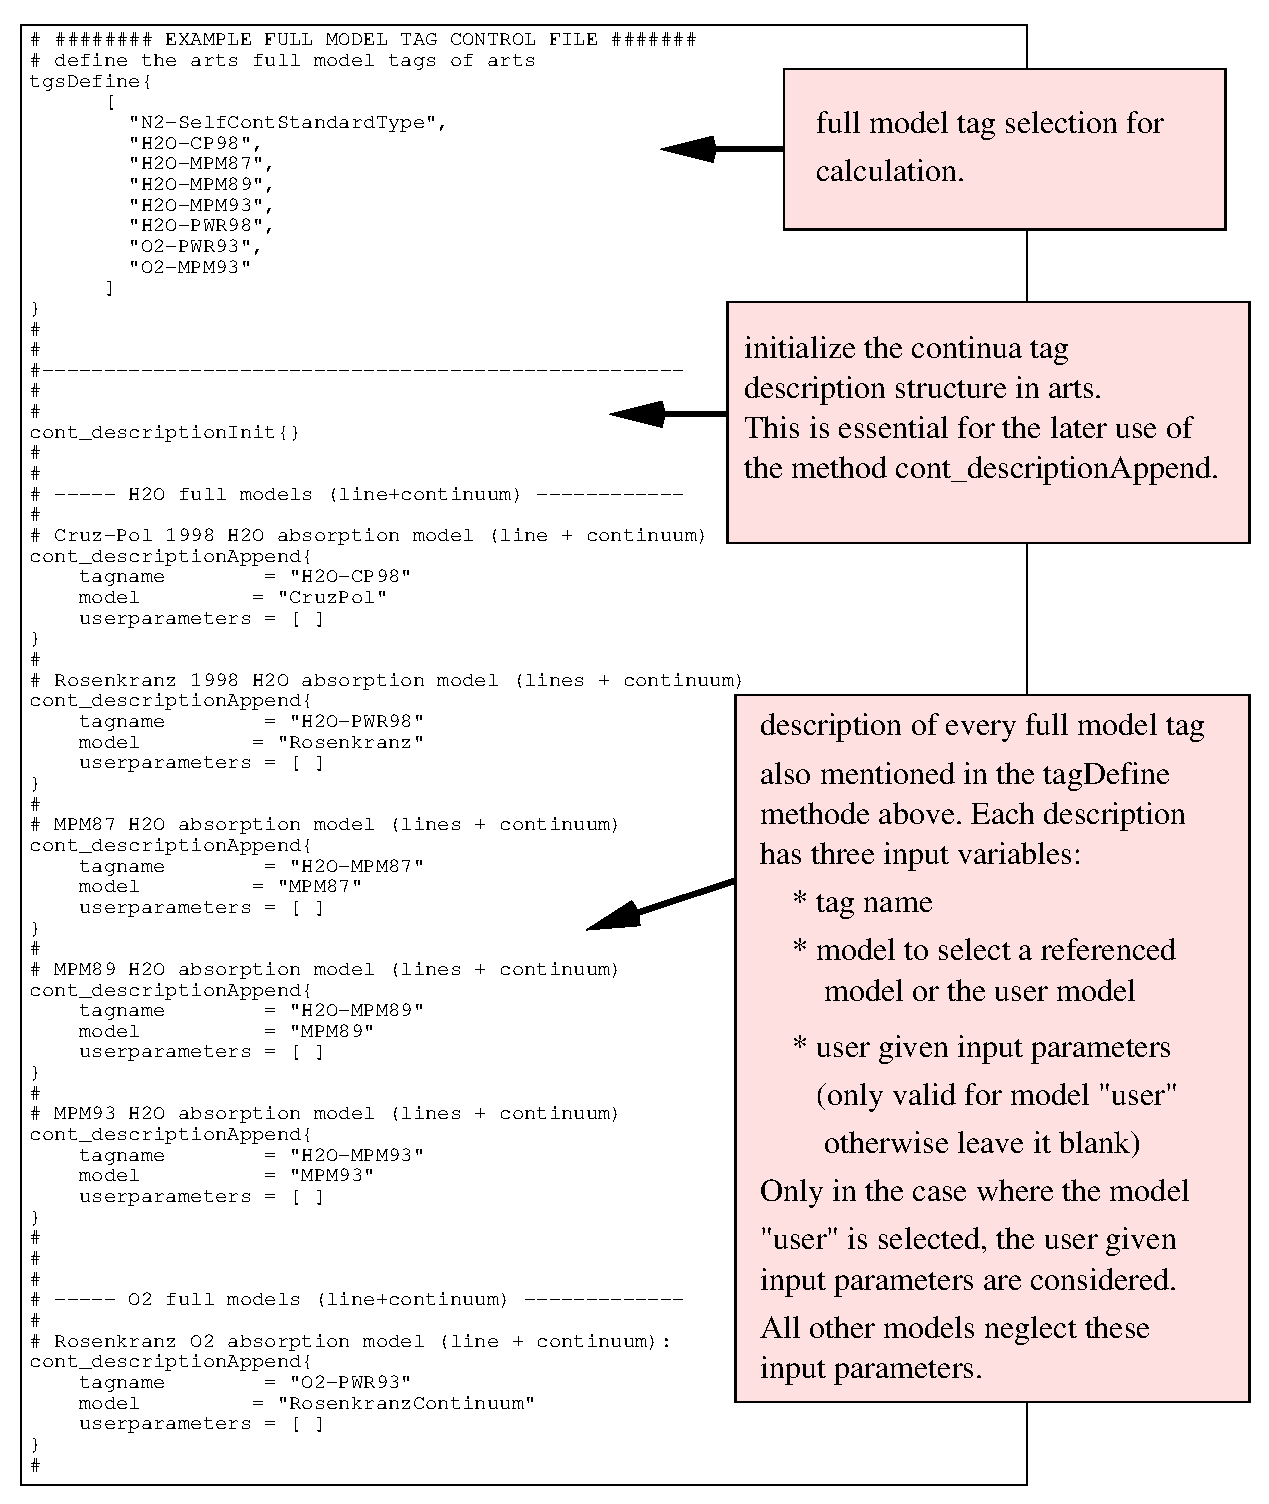
\includegraphics[scale=0.65, angle=0]{fullmodel_description_page1}
\end{flushleft}
\begin{flushleft}
 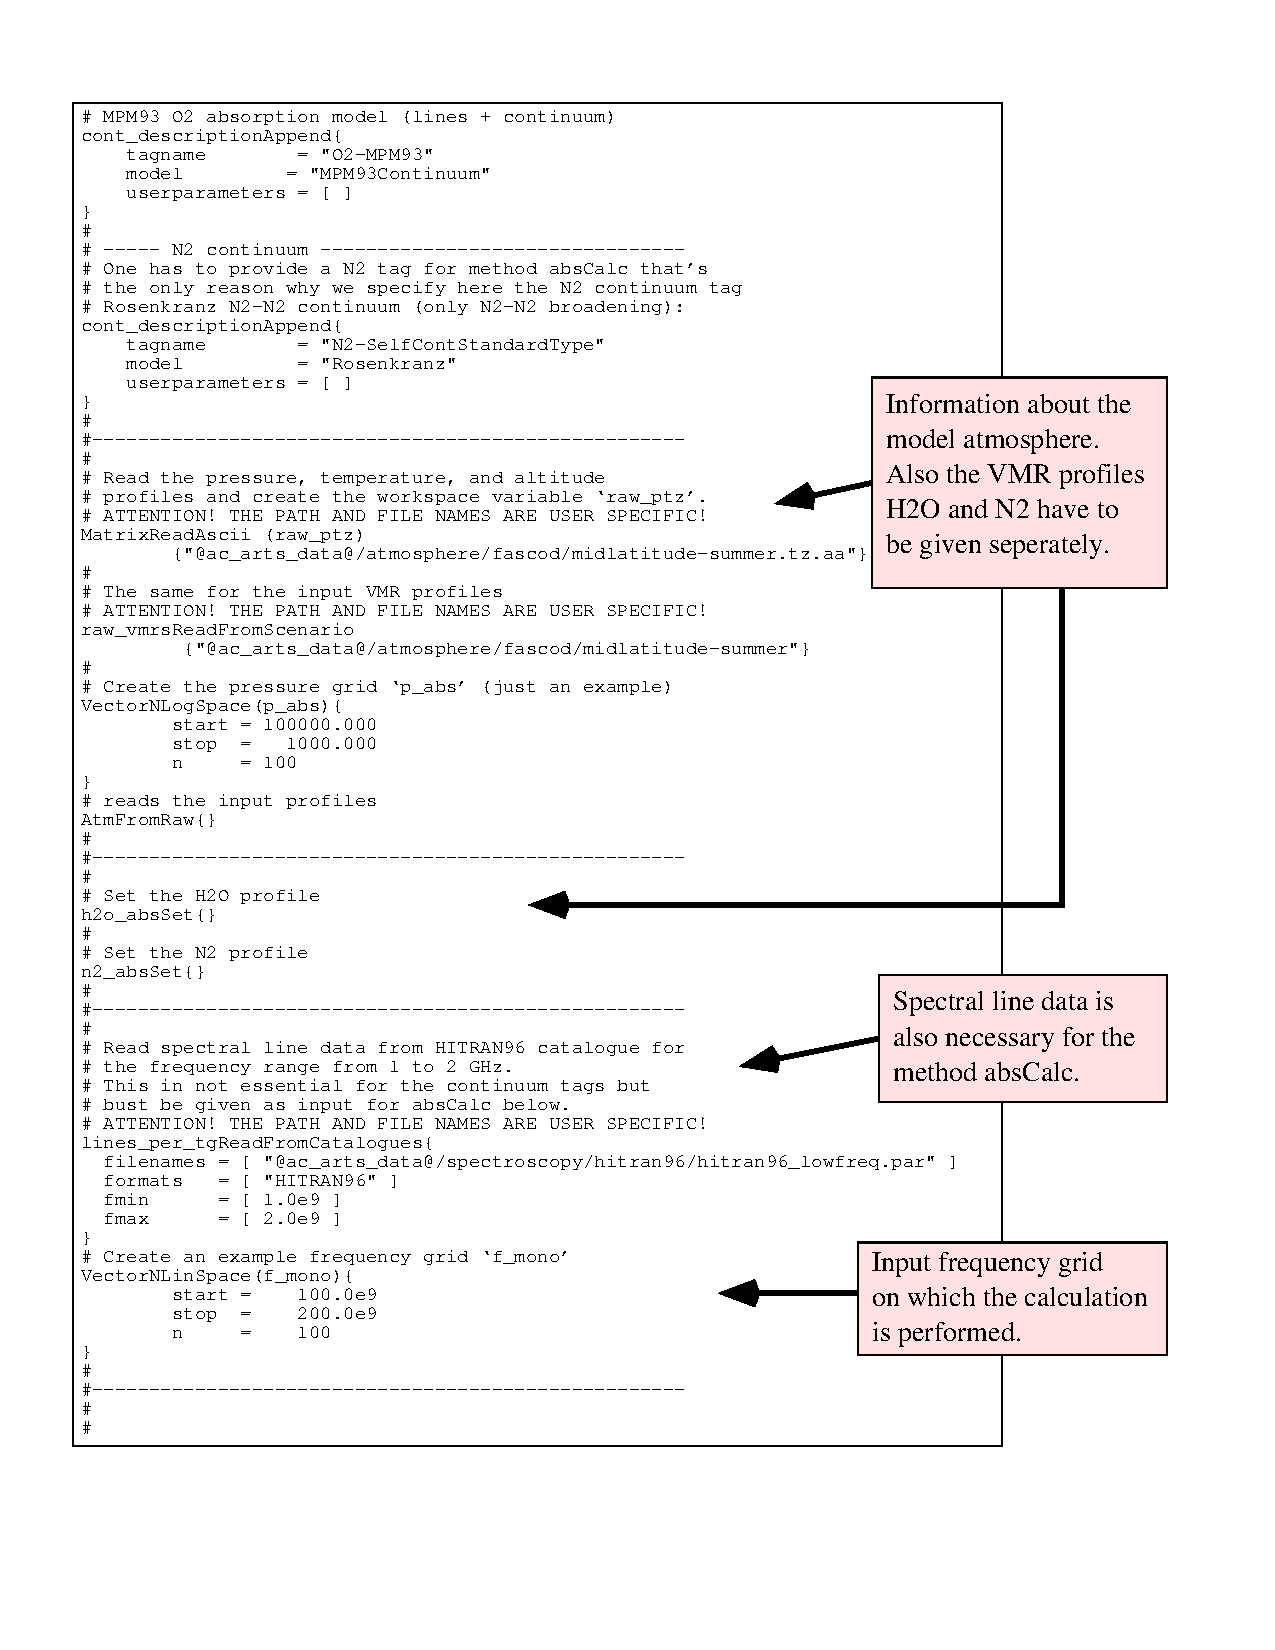
\includegraphics[scale=0.65, angle=0]{fullmodel_description_page2}
\end{flushleft}
\begin{flushleft}
 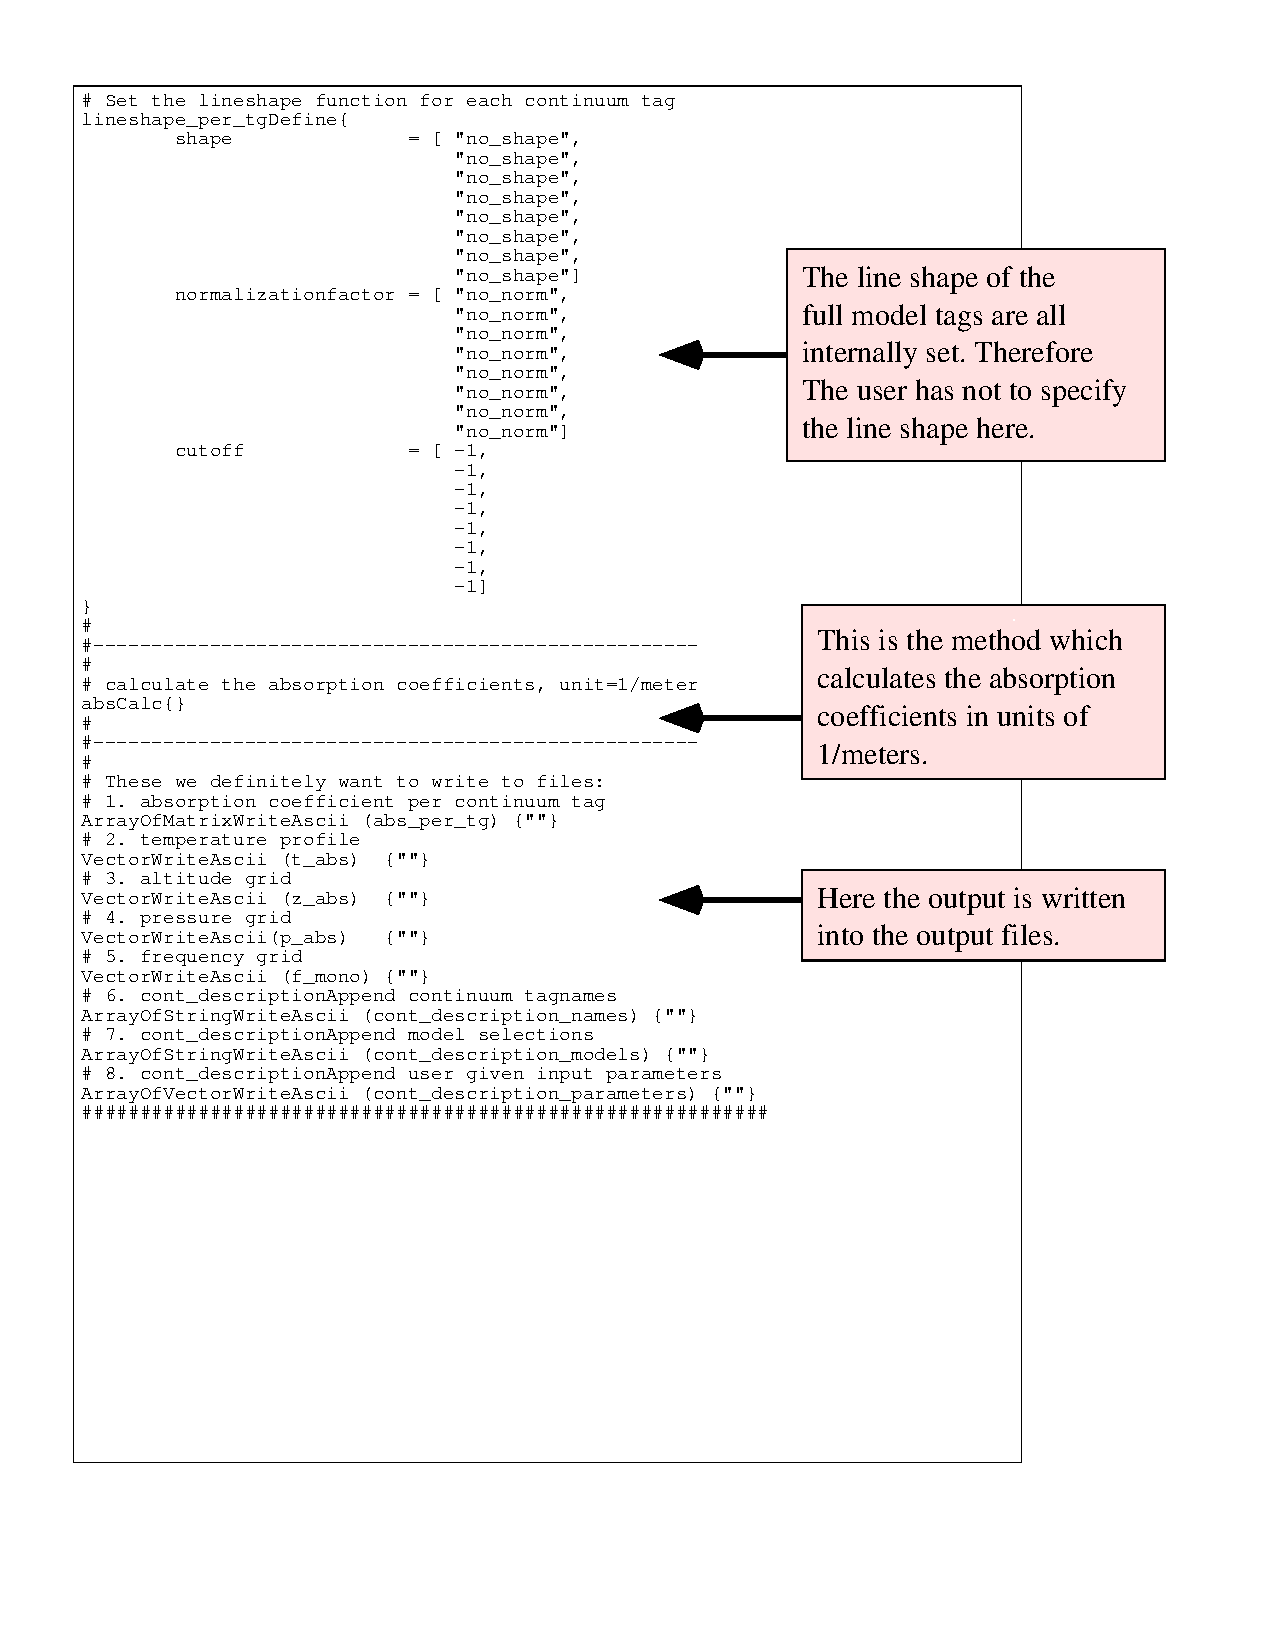
\includegraphics[scale=0.65, angle=0]{fullmodel_description_page3}
\end{flushleft}






%############################################################################# 

% ================================================================================
% The following section is written by Thomas Kuhn, iup Bremen, tkuhn@uni-bremen.de
% ================================================================================

\levela{Cloud Absorption}
\label{labela:cloudabsorption}
%=============================

\levelb{Liquid water and ice particle absorption}
\label{levelb:lipartabs}
%*************************************************
So far only absorption due to air was described. However 
hydrometeors\footnote{We denote liquid water and ice particles, either
  suspended or precipitating, in the air as hydrometeors.}
can have a noticeable effect on the radiative transfer through the
atmosphere in the 10-30\,GHz frequency range.

The MPM93 model provides beside the absorption model of air also an
absorption model for suspended liquid water droplets and ice particles
\citep{liebe:89b,liebeetal:91,hufford:91,liebeetal:93}.  The model is
applicable for the Rayleigh regime, for which the relation $r <
0.05\cdot \lambda$ holds where $r$ is the particle radius and
$\lambda$ is the wavelength\footnote{See \citet{brussaard:95}, page
  81, for details.}, e. g. for a frequency of around 22\,GHz 
this means $r<$~500\,$\mu$m. Considering \citet{salby:96}, this criterium is --
except for cirrus -- nearly for every aerosol and cloud class
satisfied. But one has to bear in mind that these values have a wide
range of variability, for example, \citet{salby:96} states that the
mean particle radius for stratus, cumulus, and nimbus clouds can be in
the range of 10-1000\,$\mu$m and that the particle radius distribution
is highly unsymmetric. 

With respect to the imaginary part of the complex refractivity, a 
unified parameterization of liquid and ice particle absorption 
is formulated in MPM93:
\begin{eqnarray}
  \label{eq:abs_cloud}
  \alpha & = & 0.1820 \cdot \nu \cdot\imn\hspace*{20mm}
               \mbox{dB/km}\\
    \imn & = & \frac{3}{2} \cdot \frac{w}{m} \cdot 
               \Im{[(\er-1)/(\er+2)]}\nonumber\\
    \imn & = & \frac{3}{2} \cdot \frac{w}{m} \cdot 
               \left[\frac{3\cdot\ime}{(\ree+2)^2~+~(\ime)^2}\right]\nonumber\\
  \nonumber
\end{eqnarray}
where $w$ is the liquid water (0.0\,$<LWC<$\,5.0\,g/m$^3$) or ice
mass (0.0\,$IWC$\,1.0\,g/m$^3$) content and $m$ is the water 
or ice bulk density ($\denli$=1.0\,g/cm$^3$ and 0.916\,g/cm$^3$, respectively).\\
The difference between liquid water and ice absorption is put in the 
expressions for the complex permittivities (i. e. the relative 
dielectric constant), $\er=\ree+i\cdot\ime$, which depend on frequency
and temperature.

\noindent$\bullet$ Complex permittivity for suspended liquid water droplets:
\begin{eqnarray}
  \label{eq:comp_perm_lwc}
  \ree       & = & \epsilon_o~-~\nu^2\cdot
                   \left[\frac{\epsilon_o-\epsilon_1}{\nu^2+\gamma_1^2}~+~
                   \frac{\epsilon_1-\epsilon_2}{\nu^2+\gamma_2^2}\right]\nonumber\\
%
  \ime       & = & \nu\cdot\left[\gamma_1\cdot
                   \frac{\epsilon_o-\epsilon_1}{\nu^2+\gamma_1^2}~+~
                   \gamma_2\cdot\frac{\epsilon_1-\epsilon_2}{\nu^2+\gamma_2^2}\right]\nonumber\\
%
  \label{eq:comp_perm_lwc_epsilon_0}
  \epsilon_o & = & 77.66 + 103.3\cdot(\Theta-1)\\
  \epsilon_1 & = & 0.0671\cdot\epsilon_o\nonumber\\
  \epsilon_2 & = & 3.52\nonumber\\
%
  \label{eq:comp_perm_lwc_gamma_1}
  \gamma_1   & = & 20.20 - 146\cdot(\Theta-1) + 316\cdot(\Theta-1)^2\,\mbox{GHz}\\
  \gamma_2   & = & 39.8\cdot\gamma_1\,\mbox{GHz}\nonumber\\
%
  \Theta     & = & 300\,\mbox{K}~/~T\nonumber
%
%  LWC        & = & 0.0~\mbox{to}~5.0~\mbox{g}/\mbox{m}^3
%                   \hspace*{10mm}\mbox{cloud liquid water content}\nonumber\\
%  \rho_l     & = & 1.0~\mbox{g}/\mbox{cm}^3
%                \hspace*{10mm}\mbox{water density}\nonumber
%  \nonumber
\end{eqnarray}
$\bullet$ Complex permittivity for ice crystals:
\begin{eqnarray}
  \label{eq:comp_perm_iwc}
  \ree    & = & 3.15\nonumber\\
%
  \ime    & = & \frac{a}{\nu}~+~b\cdot\nu\nonumber\\
%
  \label{eq:comp_perm_iwc_a}
  a       & = & (\Theta-0.1871)\cdot\exp{(17.0-22.1\cdot\Theta)}\\
  \label{eq:comp_perm_iwc_b}
  b       & = & \left[\left(\frac{0.233}{1-0.993/\Theta}\right)^2 + 
                \frac{6.33}{\Theta} - 1.31\right]\cdot10^{-5}\\
%
  \Theta  & = & 300\,\mbox{K}~/~T\nonumber
%
%  IWC     & = & 0.0~\mbox{to}~1.0~\mbox{g}/\mbox{m}^3 
%                \hspace*{10mm}\mbox{cloud ice water content}\nonumber\\
%  \rho_i    & = & 0.916~\mbox{g}/\mbox{cm}^3
%                \hspace*{10mm}\mbox{ice density}\nonumber
%  \nonumber
\end{eqnarray}
%
The absorption is directly proportional to the liquid or ice water
content $LWC/IWC$ and inversely proportional to the density of a
single liquid ice particle $\denli$. Like the mean particle radius,
the liquid and ice water content have a high variability. Table
\ref{tab:lwc} reflects this variability by summarizing different
literature values for several cloud types. Additional uncertainty 
of this absorption term comes from two sides: 
(1) the difference to the Rayleigh approximation
of the order of 1-6\% as reported in \citet{lietal:97} and (2) from
the fit of the complex permittivity.  Since $\epsilon(\nu,T)$ was
fitted to measurements which were mostly performed above $0^\circ$C,
the extrapolated values for $T<$0$^{\rm o}$C for super-cooled
clouds are not well established. For example in \cite{liebeetal:91} 
itself two different parameterizations for the so called primary 
relaxation frequency ($\gamma_1$ in Equation \ref{eq:comp_perm_lwc}) 
are given, one polynomial in $\Theta$ as presented in 
Equation \ref{eq:comp_perm_lwc}) and an exponential function derived
from theory. Although the polynomial describes the selected 
data better than the exponential function, this might not be true for
temperatures well below 0$^{\rm o}$C.
The difference in $\gamma_1$ according to these two approaches can 
be more than 2\,GHz for very low temperatures \citep{liptonetal:99}. 
The resulting consequences from this discrepancy for the absorption 
calculation at three microwave frequencies are shown in 
Figure \ref{fig:refrac_water_comp}. A more detailed
discussion about this source of uncertainty is given in Section
\ref{levelb:ref_uncert_clouds}.
%
\begin{table}[!htb]
\begin{center}
\begin{tabular}{llll}
\hline
\multicolumn{4}{c}{liquid water content ($LWC$)} \\
 cloud        & class & \multicolumn{1}{c}{(g/m$^3$)} & reference\\
\hline
 stratus      & St    & 0.15        & \cite{salby:96}\\
              &       & 0.09-0.9    & \cite{seinfeld:98}\\
              &       & 0.28-0.3    & \cite{hess:98}\\
              &       & 0.29        & \cite{abreu:96}\\
 nimbostratus & Ns    & 0.4         & \cite{salby:96}\\
              &       & 0.65        & \cite{abreu:96}\\
              &       & 0.05-0.3    & \cite{berton:00}\\
 altostratus  & As    & $<$0.01-0.2 & \cite{seinfeld:98}\\
              &       & 0.41        & \cite{abreu:96}\\
              &       & 0.1-1       & \cite{berton:00}\\
 stratocumulus& Sc    & 0.3         & \cite{salby:96}\\
              &       & $<$0.1-0.7  & \cite{seinfeld:98}\\
              &       & 0.15        & \cite{abreu:96}\\
              &       & $<$0.5      & \cite{pawlowskaetal:00}\\
              &       & 0.05-1      & \cite{berton:00}\\
 cumulus      & Cu    & 0.5         & \cite{salby:96}\\
              &       & 0.26-0.44   & \cite{hess:98}\\
              &       & 1.00        & \cite{abreu:96}\\
 cumulonimbus & Cb    & 2.5         & \cite{salby:96}\\
              &       & 0.1-2       & \cite{berton:00}\\
 cumulus 
    congestus & Cg    & 0.1-3.2     & \cite{berton:00}\\
FIRE-ACE      & -     & $<$0.7      & \cite{shupeetal:00}\\
\hline
\multicolumn{4}{c}{}  \\
\multicolumn{4}{c}{ice water content ($IWC$)}  \\
 cloud        & class & \multicolumn{1}{c}{(g/m$^3$)} & reference\\
\hline
 cirrus       & Ci    & 0.025                         & \cite{salby:96}\\
              &       & 0.00193-0.0260                & \cite{hess:98}\\
              &       & 3.128$\cdot$10$^{-4}$-0.06405 & \cite{abreu:96}\\ 
              &       & 0.15-0.3                      & \cite{larsenetal:98}\\
              &       & $<$0.1                        & \cite{berton:00}\\
cirrostratus  & Cs    & 0.2                           & \cite{salby:96}\\
              &       & 0.05-2                        & \cite{berton:00}\\
\hline
\end{tabular}
\caption{Stated values for the liquid and ice water content of several 
  cloud classes from different sources.}
\label{tab:lwc}
\end{center}
\end{table}



\levelb{Variability and Uncertainty in Cloud Absorption}
\label{levelb:ref_uncert_clouds}
%--------------------------------------------------------
In the case of clouds three sources of uncertainties can be considered
at first sight: (1) validity of the Rayleigh approximation (2) the 
parameterization of the relative dielectric constants ($\er$) of water 
and ice in the microwave region, and (3) the statistical and
climatological variability of the cloud liquid water and ice content.

As it was stated above (Section \ref{levelb:lipartabs}) the Rayleigh 
approximation is valid for particle sizes $<$~500\,$\mu$m. Figure 
\ref{fig:cloud_part_dist} shows a particle size distribution for water
clouds and ice clouds (cirrus) from the OPAC model \citep{hess:98}. 
According to this model only cirrus clouds will have particles of size
larger than 500\,$\mu$m. Nevertheless one has to keep in mind that the
variability of the particle size can be very high so that at certain 
conditions some cloud types (most probable is the cumulonimbus) 
a non-negligible large particle concentration can occur.

The uncertainty in the relative dielectric constant of water 
(see e.~g. \citet{liptonetal:99}) is largest below the freezing 
temperature, since only a few measurements at -4$^{\rm o}$C 
contributed to the parameterization of $\er$ in \cite{liebeetal:91}, 
which in turn is used in the cloud liquid water absorption model of MPM93. 
Figure \ref{fig:refrac_water_comp} shows a comparison of 
\cite{liebeetal:91} and \cite{ray:72}\footnote{{The calculations
  for this parameterizastion are performed with the computer code}\\{
   of W. Wiscombe, NASA, GSFC}\\
  (ftp://climate.gsfc.nasa.gov/pub/wiscombe/Refrac\_Index/WATER/)
  For the microwave frequency range this program uses the
  \cite{ray:72} temperature parameterization.} parameterizations 
for the temperature dependence of the expression
$\Im{[(\er-1)/(\er+2)]}$, which is in the Rayleigh approximation 
one of the relevant terms in the absorption calculation (see 
Equation \ref{eq:abs_cloud}). Additionally the same calculations with 
the alternative expression of the first  relaxation frequency, 
$\gamma_1$, as stated in Equation~2b of \cite{liebeetal:91} is shown. 
The three versions give comparable results for temperatures warmer 
than 260\,K but show significant  differences for temperatures below 
240\,K. However, an uncertainty estimation of $\Im{[(\er-1)/(\er+2)]}$ 
is due to the lack of measurements not easy, but it will certainly
increase with decreasing temperature.

The largest variability of the involved quantities of cloud absorption
is the liquid and ice water content ($LWC$ and $IWC$) of the clouds 
(see Table \ref{tab:lwc}). Even within a single cloud the $LWC$ ($IWC$) changes
with altitude and the distance from the cloud center as can be seen for
example in Figure 10 of \citet{ludlammason:57} and in the model study
of \citet{costaetal:00}.




\levelb{Water Vapor Saturation Adjustment in the Cloud}
\label{levelb:WV_sat_in_cloud}
%--------------------------------------------------------

The arts method {\tt WaterVaporSaturationInClouds{}} assures that 
the water vapor partial pressure is automatically set to 
saturation pressure (100\,\% relative humidity) in the cloud vertical
range.
This method sets the water vapor partial pressure to the 
saturation pressure over liquid water in case where liquid clouds 
are present and to the saturation pressure over ice where 
ice or water/ice clouds are present. The calculation of the 
saturation pressure is calculated according to the 
Goff-Gratch approximation \citep{liebeetal:93}:

\begin{eqnarray}
  \theta &=& (373.16\,\mbox{K} / T) \\
%
  x      &=& A \cdot \left(\theta -1 \right) + 
             B \cdot \log{(\theta)} + \nonumber\\ 
         &&  C \cdot \left( 10^{d\cdot (1- \theta^{-1})} -1 \right) +  
             E \cdot \left( 10^{g\cdot (\theta-1)} -1 \right) \\ 
%
  e^w_s  &=& 101324.6 \cdot 10.0^x\,\mbox{Pa} 
\end{eqnarray}
with
\begin{eqnarray}
 A &=& -7.90298 \nonumber \\
 B &=& 5.02808  \nonumber \\
 C &=& -1.3816 \cdot 10^{-7} \nonumber \\
 d &=& 11.344 \nonumber \\
 E &=& 8.1328 \cdot 10^{-3} \nonumber \\
 g &=& -3.49149 \nonumber
\end{eqnarray}


The $\hzo$ saturation pressure over ice the Goff-Gratch 
approximation \citep{liebeetal:93} is as follows:
\begin{eqnarray}
  \theta &=& (273.16\,\mbox{K} / T) \\
%
  x      &=& A \cdot \left(\theta -1 \right) + 
             B \cdot \log{(\theta)} + 
             C \cdot \left( 1- \theta^{-1} \right) \\ 
%
  e^i_s  &=& 610.71 \cdot 10.0^x\,\mbox{Pa} 
\end{eqnarray}
with
\begin{eqnarray}
 A &=& -9.09718  \nonumber \\
 B &=& -3.56654  \nonumber \\
 C &=&  0.876793 \nonumber
\end{eqnarray}



\begin{figure}[!htb]
  \begin{center}
% ---- uncertainty -------------------------------------
%   \includegraphics*[scale=0.6, angle=90, viewport= 80 725 480 70]%
   \includegraphics*[width=0.6\hsize, angle=90]%
   {LWCcloud}\\
% ---- ratio -------------------------------------------
%   \includegraphics*[scale=0.6, angle=90, viewport= 80 725 480 66]%
   \includegraphics*[width=0.6\hsize, angle=90]%
   {IWCcloud}
% ------------------------------------------------------
  \end{center}
  \caption{Cloud particle size distributions according to 
    Equations~3a and 3c and the microphysical properties are from the 
    Tables 1a and 1b of the OPAC model \cite{hess:98}. 
    For the liquid water clouds (upper plot) a modified gamma 
    distribution is assumed whereas for the ice clouds (lower plot) 
    exponential functions are taken.}
  \label{fig:cloud_part_dist}
\end{figure}
%
%
\begin{figure}[!hbt]
  \begin{center}
% ---- comparison --------------------------------------
   \includegraphics*[width=0.75\hsize, angle=0]%
   {refractive_water_comp_T}
% ------------------------------------------------------
  \end{center}
  \caption{Comparison of the imaginary part of the expression 
    \mbox{$(\er-1)/(\er+2)$} for liquid water at the three 
    frequencies of 32.9, 22.6, and 10,3 GHz. Plotted are the two common
    models of \cite{liebeetal:91} (a) and \cite{ray:72} (b). 
    The Ray parameterization is calculated with the F77 program 
    of W. Wiscombe, NASA, GSFC, take from 
    ftp://climate.gsfc.nasa.gov/pub/wiscombe/Refrac\_Index/WATER/.
    Additionally the \cite{liebeetal:91} parameterization (c) with the 
    alternative expression for the first relaxation frequency, 
    $\gamma_1 = 20.1\cdot\exp{[7.88\cdot(1-\Theta)]}$, is plotted.}
%
%    $(\er-1)/(\er+2)$ for liquid water at the three WATS frequencies
%    of interest. Plotted are the two common
%    models of \cite{liebeetal:91} and \cite{ray:72} (calculated with 
%    the F77 program of W. Wiscombe (NASA, GSFC) take from 
%    ftp://climate.gsfc.nasa.gov/pub/wiscombe/Refrac\_Index/WATER/).}
  \label{fig:refrac_water_comp}
\end{figure}




\levelb{ARTS Workspace Variables and Methods}
\label{levelb:ArtsImplementationCloudAbsorption}
% ----------------------------------------------

This section explains how the above described cloud absorption models
are represented in the structure of the arts source code and how 
one can invoke them in the arts control file.

The cloud tags needs not necessarily more input information than 
normal trace gas tags, since both need only a profile. But to have 
more flexibility one can run these absorption models as black boxes 
or with some user given input. In connection with this input parameters 
we distinguish generally two types, the referenced models which 
are taken from the literature (e. g. \cite{liebeetal:93}) and the 
user model, for which the arts user is providing the necessary 
parameter values.

Formally the cloud tags are like the 
continuum or full model tags implemented. Therefore after selecting 
the cloud tag with the {\tt tagDefine} method, the arts user has to 
setup the arts internal structure (i. e. the workspace variables 
{\it cont\_description\_names, cont\_description\_models, 
and cont\_description\_parameters}) for the selected continuum tags, 
which can simply be done by putting the following line into the 
arts control file:
\begin{verbatim}
cont_descriptionInit{}
\end{verbatim}

After this initialization, the cloud tag specific
information has to be transfered to arts. This is possible with the 
arts method {\it cont\_descriptionAppend}, which has itself 
three input variables: {\it tagname}, {\it model}, and 
{\it userparameters}. The user has to specify these input 
variables in the arts control file for each selected cloud tag. 
Below is a list of all the implemented continuum tags and the associated
valid range of the input variables for {\it cont\_descriptionAppend}. 
For an overview of the possible continuum tags and their 
referenced models see Table \ref{tab:artscloudlist} and the 
online documentation can be found under 
{\it arts/doc/doxygen/html/continua\_cc.html}.

One has to note at this place that the two input variables {\it model} and
{\it userparameters} are to some extend redundant. Therefore one can also 
produce an ambiguity by giving contradicting values for these two input variables.
To avoid such ambiguities the arts user should keep in mind the general 
rule that only the user model ({\it model ="user"}) needs input parameters 
via the input variable {\it userparameters}. The referenced models 
need no input via {\it userparameters}. If you try to run the arts control 
file with a referenced model and input parameters you will get an error message.
Below in the detailed description of {\it cont\_descriptionAppend} you 
can find correct examples for all the cloud tags.

\begin{itemize}
\item[$\bullet$] The liquid water cloud absorption model of 
     MPM93 \citep{liebeetal:93} has the arts tag name 
     {\tt "liquidcloud-MPM93"}. The details about this 
     absorption model are described in Section 
     \ref{labela:cloudabsorption}. The standard way to use 
     the MPM93 liquid water cloud absorption model is to set 
     the input variable {\it model} to "MPM93" and leaving 
     the input parameter {\it userparameters} empty. \\ To 
     have a minimum possibility of variation one can also run 
     this tag with {\it model}\,=\,"user". In this case one 
     has to provide three input parameters via {\it userparameters}, 
     e. g. {\it userparameters}\,=\,$[CC$, $CG$, $CE]$. The first 
     input parameter ($CC$) scales the total liquid water cloud absorption 
     (see Eq. \ref{eq:abs_cloud}) while $CG$ scales the first 
     relaxation frequency, $\gamma_1$, (see Eq. 
     (\ref{eq:comp_perm_lwc_gamma_1})) and  $CE$ scales $\epsilon_o$ 
     (see Eq. \ref{eq:comp_perm_lwc_epsilon_0})
\begin{verbatim}
cont_descriptionAppend{
    tagname        = "liquidcloud-MPM93"
    model          = "MPM93"
    userparameters = [ ]
}
cont_descriptionAppend{
    tagname        = "liquidcloud-MPM93"
    model          = "user"
    userparameters = [ 1.0, 1.0, 1.0 ]
}
\end{verbatim}
\item[$\bullet$] The ice water cloud absorption model of 
     MPM93 \citep{liebeetal:93} has the arts tag name 
     {\tt "icecloud-MPM93"}. The details about this 
     absorption model are described in Section 
     \ref{labela:cloudabsorption}. The standard way to use 
     the MPM93 ice water cloud absorption model is to set 
     the input variable {\it model} to "MPM93" and leaving 
     the input parameter {\it userparameters} empty. \\ To 
     have a minimum possibility of variation one can also run 
     this tag with {\it model}\,=\,"user". In this case one 
     has to provide three input parameters via {\it userparameters}, 
     e. g. {\it userparameters}\,=\,$[CC$, $CA$, $CB]$. The first 
     input parameter ($CC$) scales the total ice water cloud absorption 
     (see Eq. \ref{eq:abs_cloud}) while $CA$ scales $a$, (see Eq. 
     (\ref{eq:comp_perm_iwc_a})) and $CB$ scales $b$ 
     (see Eq. \ref{eq:comp_perm_iwc_b})
\begin{verbatim}
# MPM93 model for ice water particle absorption:
cont_descriptionAppend{
    tagname        = "icecloud-MPM93"
    model          = "MPM93"
    userparameters = [ ]
}
# MPM93 model for ice water particle absorption:
cont_descriptionAppend{
    tagname        = "icecloud-MPM93"
    model          = "user"
    userparameters = [ 1.0, 1.0, 1.0 ]
}
\end{verbatim}
\end{itemize}


Another important point is to state in the arts control file which
cloud profile should be read in. Becasue for a single climate zone one
can have several different cloud types, it is not enough to state 
e. g. just {\it midlatitude-summer} or {\it tropical} as for 
trace gases. Therefore the method {\tt raw\_vmrsReadFromFiles} has to 
be used to read in the trace gas and clooud profiles. For example 
the following lines in the control file will read in trace gas 
profiles from a midlatitude-summer scenario (this information is
provided with the input variable {\it basename} which states the 
basic scenario) and cumulonimbus and cirrus cloud profiles for 
liquid water and ice water clouds, respectively:
\begin{verbatim}
# ATTENTION! THE PATH AND FILE NAMES ARE USER SPECIFIC!
raw_vmrsReadFromFiles
  {seltags   = [ "liquidcloud-MPM93", 
                 "icecloud-MPM93" ]
   filenames = [ "cumulonimbus.MPM93droplet.aa",
                 "cirrus.MPM93ice.aa" ]
   basename  =   "midlatitude-summer"
  }
#
\end{verbatim}
The method {\tt raw\_vmrsReadFromFiles}can be used for any tag and 
is not specific for cloud tags. In general one has to state in the 
input variable {\it seltags} the tags which take their profile 
information from the files stated in the input variable 
{\it filenames}, while all the tags which are not stated in 
{\it seltags} take their profile information, i. e. the atmospheric 
scenario, from the input variable {\it basename}. 

To set the water vapor pressure in the cloud range to the saturation 
pressure you can use the method {\tt WaterVaporSaturationInClouds{}}
after the call of the method {\tt AtmFromRaw{}}. The saturation
pressure is calculated over liquid water in liquid water clouds and
over ice in ice water clouds. If both cloud types are present the
saturation over ice is taken.

\begin{landscape}
 \setlength{\LTcapwidth}{180mm} % with of the caption in longtable
 \begin{longtable}{llllll}
 K & K & K & K & K & K \kill
%
% --------------------- only begin of table ------------------------------
 \hline
 continuum & \multicolumn{3}{c}{{\it cont\_descriptionAppend} input} & 
 reference/ & arts source code function\\
 & \multicolumn{3}{c}{input parameter} & arts uguide & \\
 \hline
 \endfirsthead
% --------------------- every page begin of table ------------------------
 \hline
 continuum & \multicolumn{3}{c}{{\it cont\_descriptionAppend}} & 
 reference/ & arts source code function\\
 & \multicolumn{3}{c}{input parameter} & arts uguide & \\
 \hline
 \endhead
% --------------------- every page end of table ------------------------
 K & K & K & K & K & K \kill
 \hline
 \caption[]{(continued)}\\
 \endfoot
% --------------------- only end of table ------------------------------
 K & K & K & K & K & K \kill 
 \hline
 \caption{This table gives an overview of the implemented referenced 
   cloud absorption models and how they are specified 
   in the arts method {\it cont\_descriptionAppend}. Additionally the 
   reference and the arts source code function names (see file 
   {\it arts/src/continua.cc} are provided. The detailed online 
   documentation can be found under 
   {\it arts/doc/doxygen/html/continua\_cc.html}).}
 \label{tab:artscloudlist}
 \endlastfoot
% --------------------- body of table  ----------------------------------  
 \multicolumn{6}{c}{{\bf water vapor ($\hzo$)}}\\
 \hline
% --------------------------------------------------------------
 MPM93       & tagname &=& {\tt "liquidcloud-MPM93"} & \cite{liebeetal:93} & 
             MPM93WaterDropletAbs\\
             & model   &=& "MPM93"    &   &  \\ 
             & userparameters &=& [ ] &   & \\
 \hline
% --------------------------------------------------------------
 MPM93       & tagname &=& {\tt "icecloud-MPM93"} & \cite{liebeetal:93} & 
               MPM93IceCrystalAbs\\
             & model   &=& "MPM93"    &   &  \\ 
             & userparameters &=& [ ] &   & \\
 \hline
% -----------------------------------------------------------------------  
 \end{longtable}
 \setlength{\LTcapwidth}{0.8\textwidth}
\end{landscape}




\leveld{ARTS Example Control File for the Full Model Tags}
\label{leveld:ArtsCloudModelExampleControlFile}
% --------------------------------------------------------
Below you will find an example of a control file for all 
the implemented cloud absorption models. At the moment only 
the MPM93 model for water and ice clouds is implemented.
Please note that to run this example control file you 
have to specify user specific paths and input file names 
to run it properly. You can find this example in the 
arts directory {\it arts/doc/examples/cloud\_example.arts}
%
\begin{flushleft}
 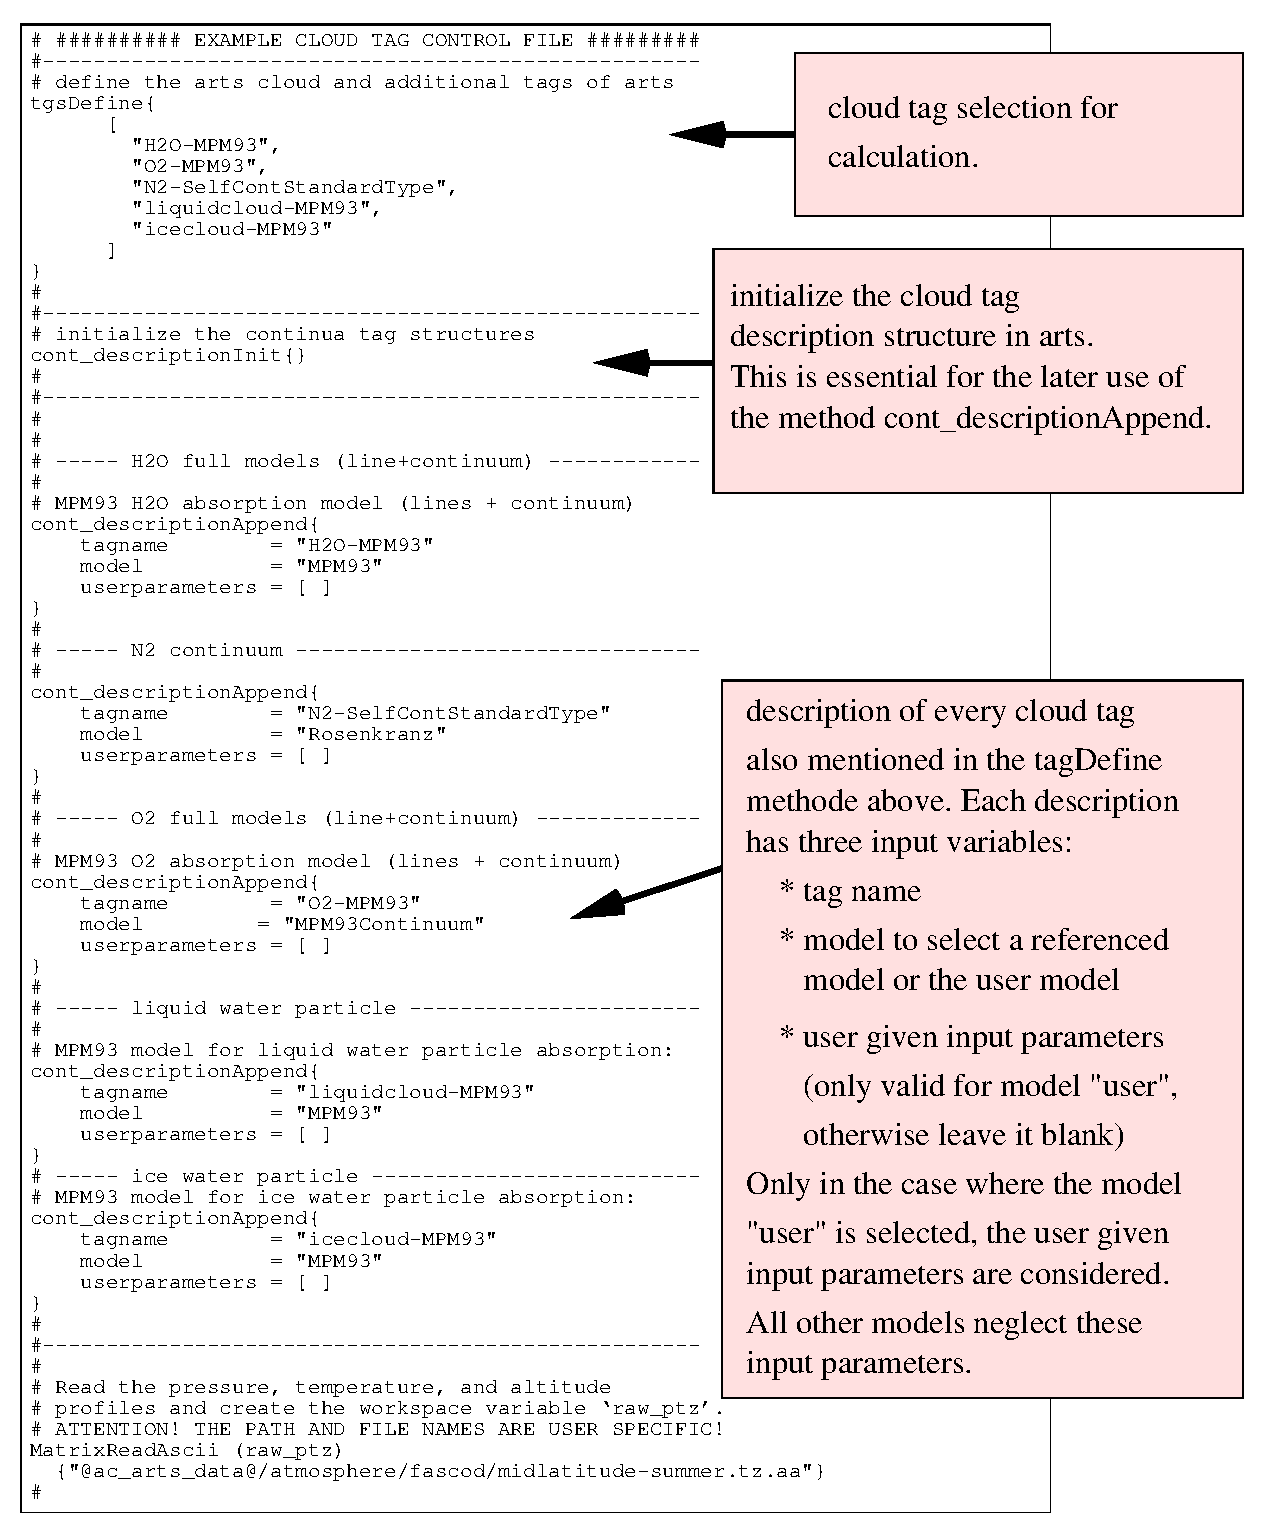
\includegraphics[scale=0.65, angle=0]{cloud_description_page1}
\end{flushleft}
\begin{flushleft}
 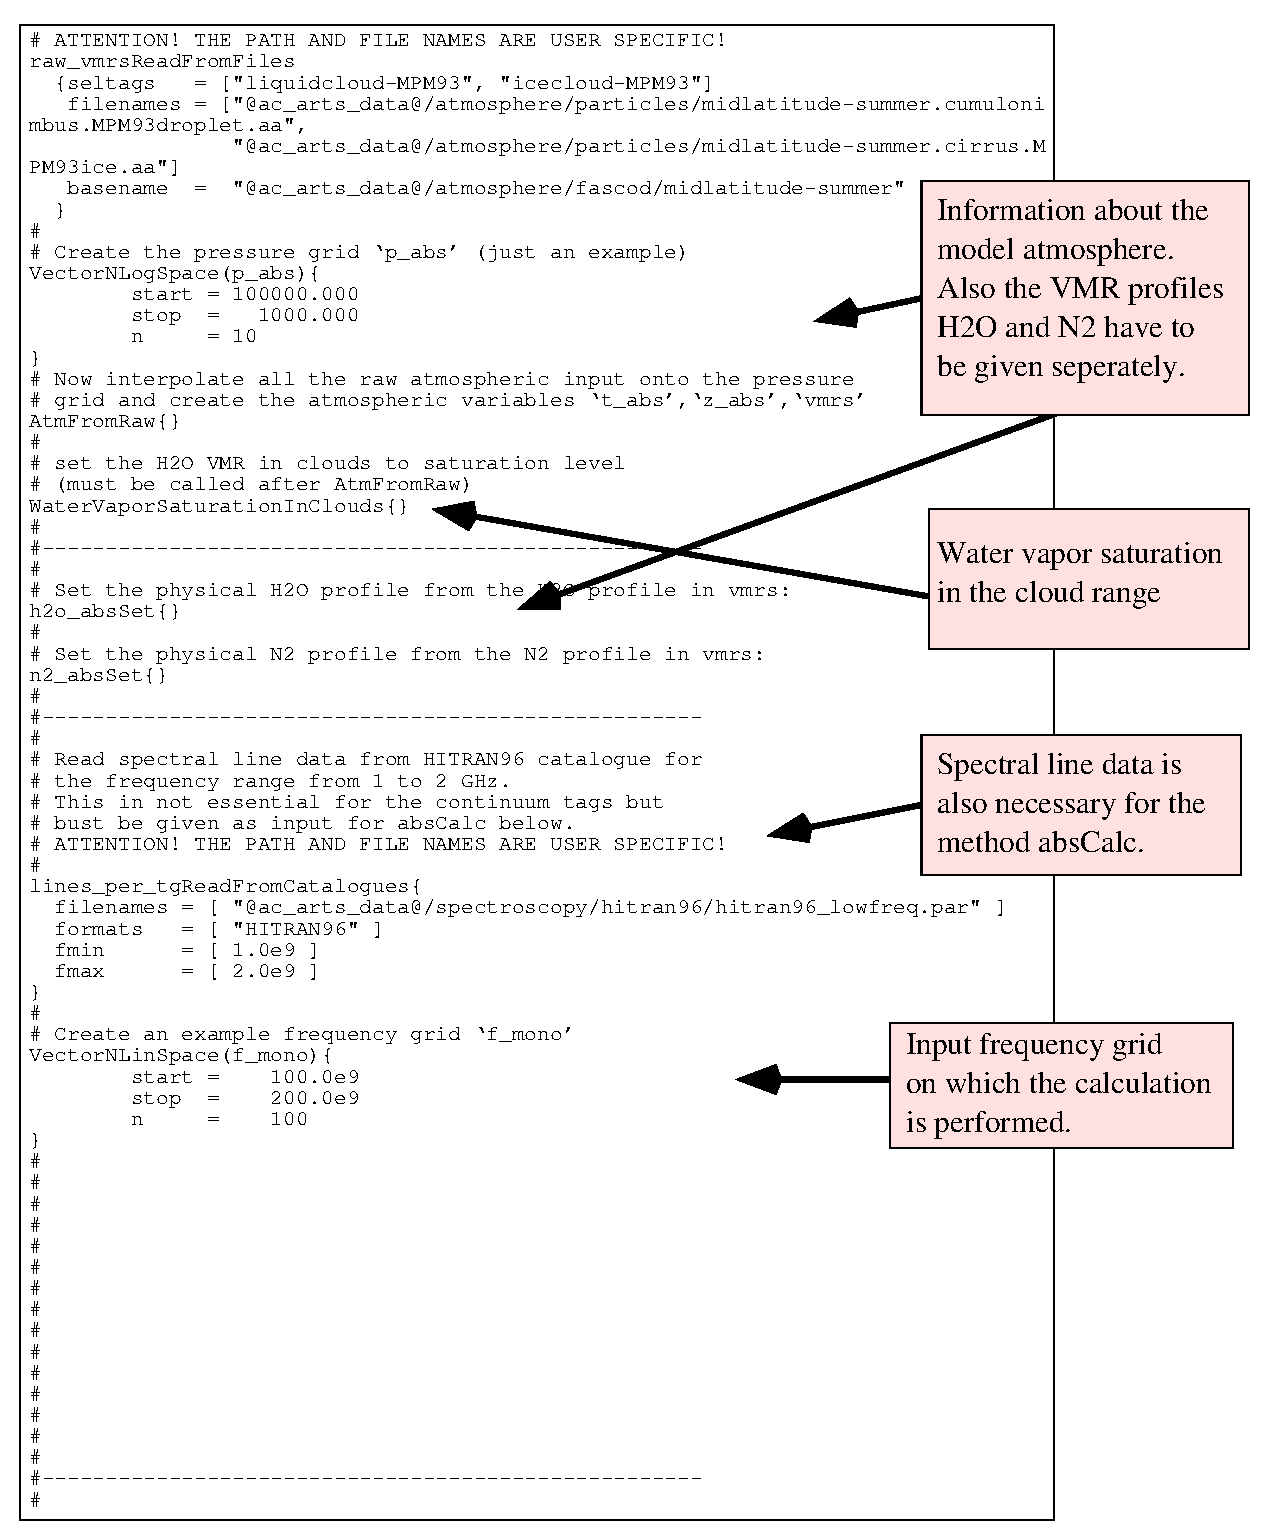
\includegraphics[scale=0.65, angle=0]{cloud_description_page2}
\end{flushleft}
\begin{flushleft}
 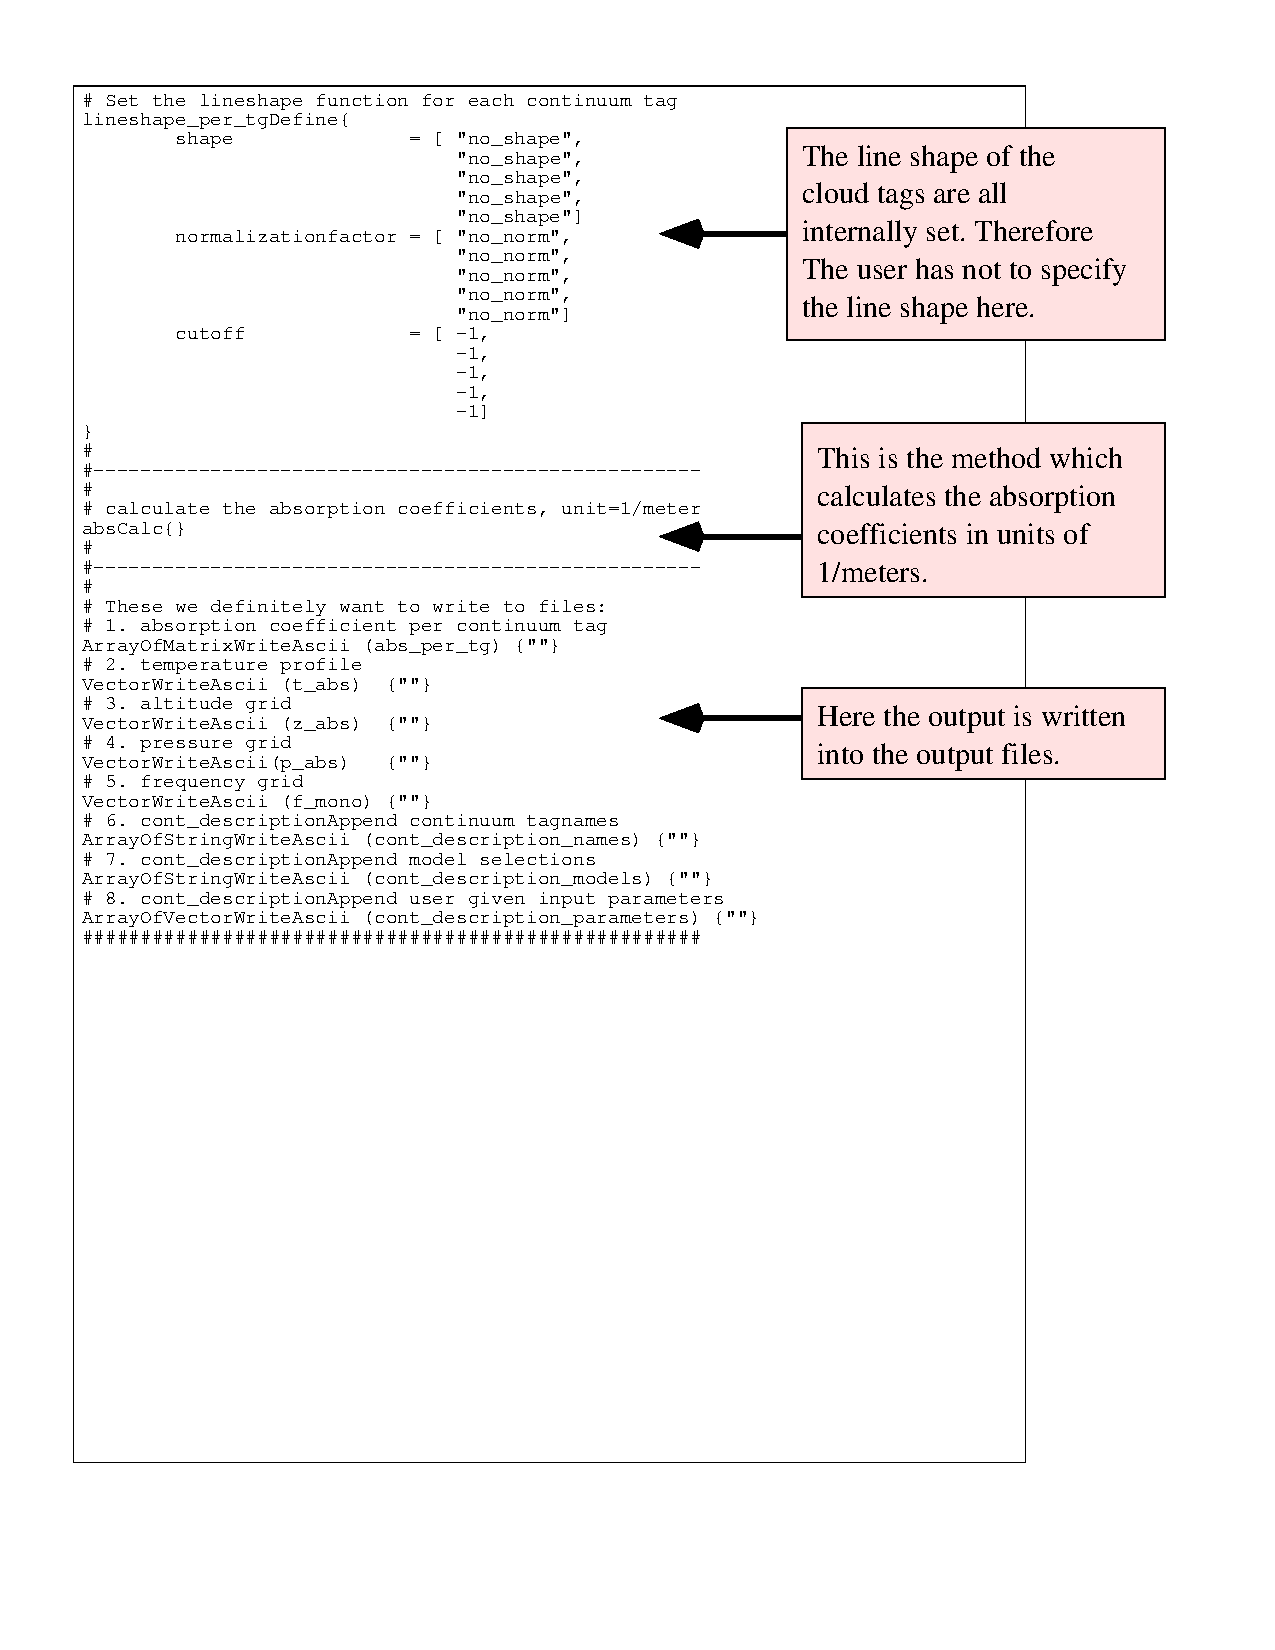
\includegraphics[scale=0.65, angle=0]{cloud_description_page3}
\end{flushleft}



%%% Local Variables: 
%%% mode: latex 
%%% TeX-master: "uguide"
%%% End:

% LocalWords:  Atmosperic

%
% To start the document, use
%  \levela{...}
% For lover level, sections use
%  \levelb{...}
%  \levelc{...}
%
\levela{Basic radiative transfer}
 \label{sec:rte}


%
% Document history, format:
%  \starthistory
%    date1 & text .... \\
%    date2 & text .... \\
%    ....
%  \stophistory
%
\starthistory
  000307 & Started by Patrick Eriksson. \\
  000908 & First version finished by Patrick Eriksson. \\
  031205 & Cooling rates added by Patrick Eriksson. \\
\stophistory



%
% Symbol table, format:
%  \startsymbols
%    ... & \verb|...| & text ... \\
%    ... & \verb|...| & text ... \\
%    ....
%  \stopsymbols
%
%
%\startsymbols
%  \mpbi     & \verb|y|       & monochromatic pencil beam intensity      \\
%  $\mpbi_1$ & \verb|y_cbgr|          & cosmic background radiation      \\
%  $\mpbi_1$ & \verb|y_ground|        & ground blackbody radiation       \\
%  $S$       & \verb|S|               & source function                  \\
%  $k$       & \verb|Abs|             & total absorption                 \\
%  $T$       & \verb|t|               & temperature                      \\
%  \f        & \verb|f|               & frequency                        \\
%  $h$       & \verb|PLANCK_CONST|    & the Planck constant              \\ 
%  $c$       & \verb|SPEED_OF_LIGHT|  & speed of light                   \\
%  $k_B$     & \verb|BOLTZMAN_CONST|  & the Boltzmann constant           \\
%  $\tau$    & -                      & optical thickness                \\
%  $\zeta$   & \verb|Tr|              & transmission between LOS points  \\
%  $\zeta^{atm} $& \verb|y|           & total atmospheric transmission   \\
%  $l$       & \verb|l|               & distance along LOS               \\
%  $\Delta l$ &\verb|lstep|           & step length along LOS            \\
%  $e$       & \verb|e_ground|        & ground emissivity                \\
%  $T_{ground} $&\verb|t_ground|      & physical temperature of the ground\\
%  $T_{cbgr}$  &\verb|COSMIC_BG_TEMP| & temperature representing cosmic  \\ 
%         &                &        background radiation                 \\
% \label{symtable:rte}     
%\stopsymbols



%
% Introduction
%
This section discusses the solution of the atmospheric radiative
transfer equation (RTE). A non-scattering atmosphere in local
thermodynamic equilibrium is assumed. 
The radiative transfer equation gives the
monochromatic (infinite frequency resolution) pencil beam (infinite
spatial resolution) spectrum. The main problem here is
how to practically and accurately estimate the (continuous) integral
in the discrete forward model.
 
The discussion treats mainly measurements of atmospheric emission. The
forward model can also handle pure absorption measurements (that is,
emission is neglected) and such observations are discussed last in the
section.

The equations of this section are valid for monochromatic pencil beam
spectra, no effects of the sensor are considered. How to
incorporate sensor effects in the spectra is discussed separately
(Sec. \ref{sec:sensor}).



\levelb{Introduction}
 \label{sec:rte:intro}
 
 Atmospheric radiative transfer can be expressed generally as
 \begin{equation}
   I = I_1e^{-\int_{l_1}^{l_2}{\kappa(l)dl}} +
        \int_{l_1}^{l_2}{\kappa(l)\sigma(l)e^{-\int_{l}^{l_2}{\kappa(l')dl'}}dl}
    \label{eq:rte:rte}
 \end{equation}
 where $I$ is the monochromatic pencil beam intensity, $l$ distance
 along the line of sight (LOS), $l_1$ the point of the considered part
 of the LOS furthest away from the sensor, $l_2$ the closest point of
 the LOS, $I_1$ the intensity at $l_1$, $\kappa$ the total absorption
 along the LOS and $\sigma$ the source function.\footnote{The symbols
   $\kappa$ and $\sigma$ are used here for the absorption and the source 
   function \emph{along} the LOS. The more commonly used symbols, $k$ and
   $S$, respectively, are used below to express the variables as
   functions of altitude.}
  
 Equation \ref{eq:rte:rte} is of general validity if $\sigma$ and $\kappa$
 consider the relevant effects, for example, scattering. However, below in
 this section it is assumed that there is no scattering and the
 atmosphere is in local thermodynamic equilibrium.
  
 Note that Eq. \ref{eq:rte:rte} is valid both for the case when the LOS is
 determined by geometrical calculations and when refraction is
 considered (the refraction changes however the LOS).
  
 With the assumptions of no scattering and local thermodynamic
 equilibrium, $\kappa$ is the summed gaseous absorption, and the source
 function equals the Planck function, $B$:
 \begin{equation}
    \sigma = B(\f,T) = \frac{2h\f^3}{c^2} \frac{1}{e^{h\f/k_B T}-1}
    \label{eq:rte:planck}
 \end{equation}
 giving the blackbody radiation for a temperature $T$ and frequency
 $\f$.
  
 If $\sigma$ is constant along the considered part of the LOS, that is, the
 temperature is constant for the case $\sigma=B$, the RTE can be solved
 analytically to give
 \begin{equation}
   I = I_1e^{-\tau} + \sigma\left(1-e^{-\tau}\right)
  \label{eq:rte:step}
 \end{equation}
 where $\tau$ is the optical thickness
 \begin{equation}
   \tau = \int_{l_1}^{l_2}{\kappa(l)dl}
 \end{equation}
 The transmission corresponding to $\tau$ is
 \begin{equation}
   \zeta = e^{-\tau}
 \end{equation}  



\levelb{Practical considerations}
 \label{sec:rte:practical}
 
 The LOS can be divided into parts in several ways. As absorption and
 temperature most likely are avaliable at some vertical grid, the most
 natural choice would be to define the LOS using this vertical grid.
 This solution is problematic for limb sounding as the ratio between
 the distance along LOS and the corresponding vertical distance
 becomes infinite at the tangent point. Another solution would be to
 base the division on $\tau$, but such a division does not guarantee
 that $T$ is close to constant inside the slabs as the vertical
 extension in some cases could be very large, and each combination of
 frequency and viewing angle should require a specific division.
  
 As a practical compromise, it was here decided to divide LOS into
 equal long geometrical steps. With this scheme the division is
 identical for all frequency components, but changes between the
 viewing angles, and should give relatively fast and straightforward
 calculations, maintaining a good accuracy. This approach has
 been applied successfully in the Odin sub-mm forward model 
 \citep{eriksson:97a,eriksson:00a}.
  
 The next question is when and how to calculate LOS and the associated
 variables. As the determination of weighting functions associated
 with the absorption needs basically the same
 quantities as RTE, it is most efficient to do this procedure only
 once and in such way that the values are suitable for both RTE and
 the weighting functions. Hence, the LOS calculations shall be a
 separate part, not included in the RTE functions. The standard use of
 the forward model should then be:
  \begin{enumerate}
    \item Calculation of absorption coefficients.
    \item Determination of LOS.
    \item Calculation of the source function and transmissions along LOS.
    \item Iteration to solve RTE.
    \item Calculation of weighting functions.
    \item Saving etc.
  \end{enumerate}
 The determination of LOS is described separately in Section \ref {sec:los}. 
  

  
\levelb{Practical solution}
 \label{sec:rte:iter}
 
 The LOS is here assumed to be defined with $n$ points where the
 distance between the points is constant (see Fig \ref{fig:rte:los}).
 There are at least two definition points of the LOS ($n\geq1$). The
 absorption and the source function are determined at the points of
 the LOS, and these values are used to calculate the transmission and a
 mean source function value for the distances between the LOS points.
 Only the later two quantities are stored.

  \begin{figure}
    \includegraphics*[width=0.98\hsize]{Figs/los}
    \caption{Schematic description of the LOS and associated variables.
      The absorption and the source function at the LOS points are
      denoted $\kappa_i$ and $\sigma_i$, respectively, while $\zeta_i$
      is the transmission between the points and $\Psi_i$ is the mean
      of neighbouring source function values. Only $\zeta$ and $\Psi$
      are stored for the later calculations. All the points are
      separated by the distance $\Delta l$ (along the LOS). The distance
      between point $i$ and $i+1$ is denoted as step $i$ of the LOS. }
    \label{fig:rte:los}  
  \end{figure}

 \levelc{Absorption and transmission}  
  \label{sec:rte:abs}
  
  The absorption is treated to vary linearly between the LOS points.
  As mentioned above, the transmission values shall be valid between the
  LOS points. With these definitions, the optical thickness associated with 
  step $i$ is
 \begin{equation}
    \tau_i = \frac{\Delta l}{2} \left( \kappa_i+\kappa_{i+1} \right),
                             \quad 1\leq i < n 
  \label{eq:rte:tau}
 \end{equation}
 The relationship between the optical thicknesses and
 the transmission is
 \begin{equation}
   \zeta_i = e^{-\tau_i}
 \end{equation}
 Note that
 \begin{equation}
   e^{-\left(\tau_1+\tau_2\dots\tau_n\right)}=\zeta_1\zeta_2\dots\zeta_n
 \end{equation}
 The absorption at the LOS points is determined from the absorption
 matrix provided by the absorption module by linear interpolation,
 using the logarithm of the pressure as altitude
 coordinate\footnote{The logarithm of the pressure is throughout the
   basic altitude coordinate in ARTS.}.


 \levelc{The source function}  
  \label{sec:rte:source}
  The source function is also basically assumed to vary linearly
  between the LOS points, but for simplicity reasons, a single
  source function value is assigned to the LOS steps:
  \begin{equation}
    \Psi_i = \frac{\sigma_i+\sigma_{i+1}}{2}, \quad 1\leq i < n
   \label{eq:rte:smean}
  \end{equation}   
  The source function at the LOS points ($\sigma$) is simply by
  interpolating linearly the temperature profile, and calculating the
  Planck function (Eq. \ref{eq:rte:planck}) for the obtained
  temperatures.
  
  To fully model that the absorption and the source function have a
  simultanous linear variation between the LOS points would give much
  more complicated analytical expressions than presented here (if even
  possible to derive?). However, the simplified approach used here
  should not influence the accuracy in any important way. This as the
  source function has, compared to the absorption, a relatively low
  variation and it can be treated to be piecewise constant when solving
  the raqdiative transfer.
  
  If long wavelengths are assumed and the source function equals the
  Planck function (Eq.  \ref{eq:rte:planck}), $\sigma$ should
  maximally vary with about a factor of 2 as the minimum and the
  maximum temperature in the atmosphere are about 150 and 300 K,
  respectively, and the relationship between $\sigma$ and temperature
  is close to linear.  This should be compared to the absorption that,
  even for a single frequency, often varies with many orders of
  magnitude.


 \levelc{Solving the radiative transfer equation}  
  \label{sec:rte:solving}
  
  With the definitions given above, the intensity at point $n$ can be
  expressed as
 \begin{equation}
   I = I_1 \prod_{j=1}^{n-1}\zeta_j + 
       \sum_{i=1}^{n-1}\left[\Psi_i(1-\zeta_i)\prod_{j=i+1}^{n-1}\zeta_j\right]
  \label{eq:rte:rteprod}
 \end{equation}
 However, an alternative approach, requiring less computer memory, is
 to follow the radiation from one slab of the atmosphere to next, and
 is the method of choice here. Following Equation \ref{eq:rte:step},
 the following iterative expression can be determined
 \citep{eriksson:97a}
 \begin{equation}
   I_{i+1} = I_i\zeta_i + \Psi_i\left(1-\zeta_i\right)\qquad i=1,2,...,n-1
  \label{eq:rte:iteration}
 \end{equation}
 where $I_i$ is the intensity reaching point $i$.
 The iteration is started by setting $I_1$ to the intensity at the 
 atmospheric limit, that is, cosmic background radiation or correspondingly.


 \levelc{Considering ground reflection}  
  \label{sec:rte:ground}

 The effect of a ground reflection is modeled as
 \begin{equation}
   I^{after} = I^{before}(1-e) + eB(\f,T_{ground})
  \label{eq:rte:ground}
 \end{equation} 
 where $e$ is the ground emission factor and $I^{before}$ and
 $I^{after}$ is the intensity before and after the reflection,
 respectively. See further Section \ref{sec:los:ground}.


\levelb{Optical thicknesses}
 \label{sec:rte:trans}
  
 The atmospheric emission can be neglected if the observation is
 performed towards a sufficiently strong source, such as the Sun, and
 the measurement gives then the total atmospheric transmission,
 $\zeta^{tot}$. When inverting such observations, the standard
 approach is to invert the optical thicknesses $(\tau)$ to obtain a
 more linear inversion problem. For this reason, the output from ARTS
 when neglecting emission was selected to be optical thicknesses
 instead of transmission values. However, as the transmission for each
 step along the LOS is stored for the emission calculations, ARTS
 calculates internally transmission spectra that are converted to
 optical thicknesses.

 This transmission is
 \begin{equation}
   \zeta^{tot} = e^{-\int_{l_1}^{l_2}{\kappa(l)dl}}
  \label{eq:rte:tottrans}
 \end{equation}
 The corresponding iterative formula used in the forward model is
 simply (cf. Eq. \ref{eq:rte:iteration})
 \begin{equation}
   \zeta^{tot} = \prod_{i=1}^{n-1}\zeta_{i}
 \end{equation} 
 It is noteworthy that the multiplication order
 is of no importance, a fact that can be used for 1D limb sounding where
 the conditions are assumed to be symmetrical around the tangent point and
 only one half of the line of sight is stored. 

 If there is a ground reflection, it is considered as
 \begin{equation}
   \zeta^{tot} = (1-e)\prod_{i=1}^{n-1}\zeta_{i}
  \label{eq:rte:tground}
 \end{equation} 
 where $e$ is the ground emission factor. 

 The optical thicknesses are finally calculated as
 \begin{equation}
   \tau^{tot} = -\ln(\zeta^{tot})
  \label{eq:rte:odepth}
 \end{equation} 



\levelb{Cooling rates}
 \label{sec:rte:coolrates}
 
 Cooling rates is an important concept for climate models and studies.
 The cooling rate gives the change in temperature due to exchange of
 radiation, keeping all variables constant. The typical unit is K/day.
 There are two balancing (more or less) effects. Absorption of
 shortwave (UV -- near IR) results in a heating of the air mass. For
 thermal IR, emission and absorption are coupled phenomena but
 exchange of thermal and far IR radiation normally results in a
 cooling effect. These two effects give together the heating rate, but
 are normally calculated seperately and are then denoted as the
 heating and cooling rate. In ARTS only the IR cooling rate is
 handled, and that only for cloud free conditions. For more details on
 heating / cooling rates, see any text book on atmospheric physics.
 
 Cooling rates are calculated by the WSM \verb|CoolingRates|. The
 method returns the spectral cooling rates for the frequencies of
 \verb|f_mono| and the pressure levels of \verb|p_coolrates|. A
 positive value here means a cooling effect (that is, the heating rate
 is not returned). The unit of values in \verb|CoolingRates| is
 K/day/Hz. Directly below follows a derivation of the expression used
 in \verb|CoolingRates|.
 
\newcommand{ \pressure}       {\ensuremath{P}}
\newcommand{ \temperature}    {\ensuremath{T}}
\newcommand{ \altitude}       {\ensuremath{z}}
\newcommand{ \timesymbol}     {\ensuremath{t}}
\newcommand{ \density}        {\ensuremath{\rho}}
\newcommand{ \heatcapacity}   {\ensuremath{c_\pressure}}

\newcommand{ \flux}           {\ensuremath{F}}
\newcommand{ \monoflux}       {\ensuremath{F_\f}}
\newcommand{ \odepth}         {\ensuremath{\tau}}
\newcommand{ \planckfunc}     {\ensuremath{B_\f}}
\newcommand{ \abscoeff}       {\ensuremath{\alpha}}

 The heating rate can be expressed as
 \begin{equation}
  \label{eq:heatrate1}
  \frac{\dd\temperature}{\dd\timesymbol} = 
         \frac{-1}{\density\heatcapacity} \frac{\dd \flux}{\dd\altitude},
 \end{equation}
 where \temperature\ is the temperature, \timesymbol\ is the time,
 \density\ is the air density, \heatcapacity\ is the heat capacitivity
 (for pressure work) and \altitude\ is vertical altitude. This is the
 expression normally used to determine cooling rates.

 The idea here is to find an expression that gives the heating rate if
 the spectral radiance as a function of zenith angle is known. 
 As a first step, Equation~\ref{eq:heatrate1} is rewritten as
 \begin{equation}
  \label{eq:heatrate2}
  \frac{\dd\temperature}{\dd\timesymbol} = 
        \frac{-1}{\density\heatcapacity} \int_0^\infty \left[
        \lim_{\Delta\altitude\gets 0}\frac{\monoflux(\altitude+\Delta\altitude)-
                \monoflux(\altitude)}{\Delta\altitude} \right] \dd\f.
 \end{equation}
 The elationship between spectral radiance and monochromatic
 flux is
 \begin{equation}
  \monoflux(\altitude) = 2\pi\int_0^\pi \mpbi(\altitude,\view)
          \cos\view \sin\view \dd\theta,
 \end{equation}
 The assumption below is that the upwelling part of $\mpbi$ is
 known at \altitude\, and the downwelling part $\mpbi$ is known at
 $\altitude+\Delta\altitude$.

 The upwelling spectral radiance at altitude $\altitude+\Delta\altitude$
 can be expressed as
 \begin{equation}
   \mpbi(\altitude+\Delta\altitude,\view) = 
       \mpbi(\altitude,\view) e^{-\odepth(\view)} +
        \planckfunc(1-e^{-\odepth(\view)}),\qquad 0\leq\view\leq\pi/2,
 \end{equation}
 where \planckfunc\ is the Planck function for blackbody radiation.
 The fact that $\Delta\altitude$ will approach zero has been
 used, which mean that \planckfunc\ and \view\ can be assumed to
 be constant between \altitude\ and $\altitude+\Delta\altitude$.
 The downwelling spectral radiance at \altitude\ is in similar way
 \begin{equation}
   \mpbi(\altitude,\view) = 
       \mpbi(\altitude+\Delta\altitude,\view) 
        e^{-\odepth(\view)} +
        \planckfunc(1-e^{-\odepth(\view)}),\qquad \pi/2<\view\leq\pi.
 \end{equation}
 Again using the fact that $\Delta\altitude\approx0$, the optical depth is
 \begin{equation}
   \odepth(\view) = \frac{\Delta\altitude}{|\cos\view|} \abscoeff
 \end{equation}
 and the transmission is
 \begin{equation}
   e^{-\odepth(\view)} = 
      1 - \frac{\Delta\altitude}{|\cos\view|} \abscoeff.
 \end{equation}
 We have then that
 \begin{eqnarray}
   & \frac{\monoflux(\altitude+\Delta\altitude)- \monoflux(\altitude)}
       {\Delta\altitude} = \frac{2\pi}{\Delta\altitude}\Big\{
     \int_0^{\pi/2} \left[ \mpbi(\altitude,\view)
          (1 - \odepth(\view)) + \planckfunc\odepth(\view)\right]
          \cos\view \sin\view \dd\view + & \nonumber \\
   & + \int_{\pi/2}^\pi \mpbi(\altitude+\Delta\altitude,\view)
          \cos\view \sin\view \dd\view - 
       \int_0^{\pi/2} \mpbi(\altitude,\view)
          \cos\view \sin\view \dd\view - & \nonumber\\   
   & -\int_{\pi/2}^\pi \left[ \mpbi(\altitude+\Delta\altitude,\view)
          (1 - \odepth(\view)) + \planckfunc\odepth(\view)\right]
          \cos\view \sin\view \dd\view  \Big\}. &
 \end{eqnarray}
 Many of the terms above cancel out and the expression above can be
 shortened to
 \begin{eqnarray}
   \label{eq:diffF}
   & \frac{\monoflux(\altitude+\Delta\altitude)- \monoflux(\altitude)}
       {\Delta\altitude} = 2\pi\Big\{
     \int_0^{\pi/2} \left[ \planckfunc -\mpbi(\altitude,\view)
           \right] \abscoeff \sin\view \dd\view + & \nonumber \\
   & +\int_{\pi/2}^\pi \left[ \planckfunc -
                \mpbi(\altitude+\Delta\altitude,\view)
          \right]\abscoeff \sin\view \dd\view  \Big\}. &
 \end{eqnarray}
 Putting Equation~\ref{eq:diffF} into Equation~\ref{eq:heatrate2}, and
 noting that
 $\mpbi(\altitude,\view)=\mpbi(\altitude+\Delta\altitude,\view)$
 for $\Delta\altitude=0$,  gives finally
 \begin{equation}
   \label{eq:heatratefinal}
    \frac{\dd\temperature}{\dd\timesymbol} = 
        \frac{-2\pi}{\density\heatcapacity} \int_0^\infty 
     \int_0^\pi \left[ \planckfunc -\mpbi(\altitude,\view)
           \right] \abscoeff \sin\view \dd\view   \dd\f.
 \end{equation}
 We can already here note that the contribution to the heating rate
 will be zero for frequencies where $\abscoeff=0$.
 
 To obtrain correct results it is crucial that \mpbi\ converges to
 \planckfunc\ when it is expected $\mpbi=\planckfunc$, which is the
 case when the absorption is very high. Considering that radiative
 transfer applies a mean value of the Planck function at the end
 points of the integration step (Eq.~\ref{eq:rte:smean}), it is not a
 good idea to compare \mpbi\ with the \planckfunc\ for the position of
 interest. This would require an extremly short radiative transfer
 step length (\verb|l_step|), a statement verified by practical
 calculations. A better solution is to replace $(\planckfunc
 -\mpbi(\altitude,\view))$ in Equation~\ref{eq:heatratefinal} by
 $(\Psi-\mpbi(\altitude,\view))$, where $\Psi$ (defined in
 Eq.~\ref{eq:rte:smean}) is the effective source function for
 radiative transfer step closest to the point of interest. This
 modification will balance the radiation budget perfectly for high
 values of $\abscoeff$ and has a small impact on the accuracy.
 However, as for all radiative transfer calculations in ARTS, reducing
 the step length will improve the calculation accuracy.
 
 

 \levelb{Control file examples}
  \label{sec:rte:cfe}
 
  See Section \ref{sec:los:cfe}.



%%% Local Variables: 
%%% mode: latex
%%% TeX-master: "main"
%%% End: 

%
% To start the document, use
%  \levela{...}
% For lover level, sections use
%  \levelb{...}
%  \levelc{...}
%
\levela{Line of sight, 1D}
 \label{sec:los}


%
% Document history, format:
%  \starthistory
%    date1 & text .... \\
%    date2 & text .... \\
%    ....
%  \stophistory
%
\starthistory
  000307 & Started by Patrick Eriksson. \\
  010219 & First version finished by Patrick Eriksson.\\
\stophistory


%
% Symbol table, format:
%  \startsymbols
%    ... & \verb|...| & text ... \\
%    ... & \verb|...| & text ... \\
%    ....
%  \stopsymbols
%
%
%\startsymbols
%  \view     & \verb|view|     & zenith angle from zenith                  \\
%  $z$       & \verb|z|       & vertical altitude                          \\
%  $z_p$     & \verb|z_plat|  & platform altitude                          \\
%  $z_t$     & \verb|z_tan|   & tangent altitude                           \\
%  $z_g$     & \verb|z_ground|& altitude of the ground                     \\
%  $z_{lim}$ & \verb|z_abs_max|& practical upper limit of the atmosphere   \\
%  $l$       & \verb|l|       & distance along LOS                         \\
%  $e$       & \verb|gr_emiss|& ground emissivity                          \\
%  $\Delta l$& \verb|l_step|  & step length along LOS                      \\
%  $l_{lim}$ & \verb|llim|    & distance from lowest LOS point to $z_{lim}$\\
%  $l_p$     & \verb|l1|      & distance used for downward observation     \\
%  $i_p$     & -              & index for platform altitude for downward obs.\\
% \label{symtable:los}     
%\stopsymbols



%
% Introduction
%
This section describes how the line of sight (LOS) is determined
for situations where the atmosphere is assumed to be horizontally
stratified, a 1D atmosphere. Expressions are given both for pure
geometrical calculations and when considering refraction.



\levelb{Definitions}
 \label{sec:los:defs}
 
 Vertical (geometrical) altitudes are denoted as $z$, pressures as $p$
 and distances along the LOS are denoted as $l$. Vertical distances
 are measured from the geoid and $l$ is the distance from the lowest
 point of the LOS. 
 
 As a 1D atmosphere is assumed here, the conditions are symmetrical
 around tangent points and points of ground reflection, and, for such
 cases, only one half of the LOS is stored for efficiency reasons.
 The points of the LOS are stored by increasing vertical altitude
 point. Index 1 corresponds accordingly to either the platform, the
 tangent point or the ground.  The internal description of the LOS is
 further described in the file \verb|los.h|.
  
 The line of sight is defined by two variables, the platform altitude,
 $z_p$, and the zenith angle, $\view$, (see Fig. \ref{fig:los1d:geoms}):

 \begin{description}
  \item[The platform altitude] is the altitude above the geoid of the
       sensor used to detect the spectrum simulated.
  \item[The zenith angle] is the angle between the zenith
       direction and the direction of observation. As an 1D atmosphere is
       assumed, there is no difference between positive and negative
       zenith angles.
  \end{description}

  \noindent
  The lower limit of the atmosphere is given by the ground altitude,
  $z_g$. The practical upper limit of the atmosphere is denoted
  $z_{lim}$ and is in the forward model determined by the highest
  point of the absorption grid. The absorption grid can
  extend below $z_g$. On the other hand, it is not allowed that any
  part of the LOS is between the lowest absorption altitude and the ground.
 
  If $\view>90^{\circ}$ the lowest point of the LOS is not the platform
  altitude, and this point is denoted as the tangent point, $z_t$. The
  angle between the LOS and the vector to the Earth center is at the
  tangent point $90^\circ$. If the tangent point is below ground
  level, $z_t$ is determined by an imaginary geometric prolonging of
  the LOS inside the Earth.

  \begin{figure}[tb]
   \begin{center}
    \includegraphics*[width=0.95\hsize]{Figs/geoms}
    \caption{Schematic description of the main variables of the 
             observation geometry and the LOS. $R_e$ is the Earth
             radius. Other variables are defined in the text.}  
    \label{fig:los1d:geoms}  
   \end{center}
  \end{figure}
  
  The forward model uses internally three main observation geometries:

  \begin{description}
  \item[Limb sounding] covers here all observations from a point
    outside the atmosphere ($z_p \geq z_{lim}$). All zenith angles are
    covered, and, for example, nadir looking observations
    ($\view=180$) are treated as limb sounding in the forward model.
    If the LOS does not pass the atmosphere ($z_{tan} \geq z_{lim}$),
    cosmic background radiation, or correspondingly, is returned.
  \item[Upward looking] signifies observation from
    within the atmosphere in an upward direction ($z_p<z_{lim}$ and
    $\view\leq90^{\circ}$). 
  \item[Downward looking] is observation from within the atmosphere in
    a downward direction ($z_p<z_{lim}$ and $\view>90^{\circ}$).
  \end{description}
 

\levelb{Outlook towards 2D}
 \label{sec:los:2d}
 So far ARTS is only capable of calculating spectra for 1D cases.
 It is planned to also handle satellite measurements with atmospheric 
 horizontal variations, but limited to observations in the orbit
 plane, here denoted as 2D observations. 
 
 For 2D observations there is no symmetry to be used, each point of
 the LOS is unique. This is also the case for 1D upward looking
 observations, and it is planned that 2D and 1D upward calculations of
 radiative transfer and weighting functions shall be performed with
 the same general functions.  The 2D case exhibits however one
 difference compared to the 1D upward case. For 2D cases there could
 be a ground reflection along the LOS, which is never the case for 1D
 upward looking observations by definition.  Note that if the 1D
 upward functions are used for 2D simulations, the point of LOS
 closest to the sensor will throughout have index 1.

 As a first preparation for the 2D calculations, the angular distances
 between the sensor and the points of the LOS, $\psi$, are stored
 beside the pressure and vertical altitudes of the points. The
 variable $\psi$ is defined to be the angle between the vectors going
 from the Earth's center to the sensor and the LOS point,
 respectively.  For cases with symmetry, the angles are valid for the
 part of the LOS furthest away from the sensor.
 


\levelb{The step length}
 \label{sec:rte:stepl}
 
 As described in Section \ref{sec:rte}, the LOS is divided into equal
 long geometrical steps, $\Delta l$. The user gives an upper limit for
 this step length. A point of the LOS is always placed at the sensor
 (if inside the atmosphere), tangent points and points of ground
 reflection, but no adjustment to the upper atmospheric limit is made.
 This gives a single fixed point for limb sounding and upward looking
 observation and $\Delta l$ is set to the value given by the user if
 the LOS has at least two definition points. If the LOS gets only one
 point with the user defined value, for example when the tangent point
 is just below the atmospheric limit, the step length is adjusted to
 the length from the fixed point of the LOS (the sensor or the tangent 
 point) and the atmospheric limit.
 
 In contrast to upward and limb sounding observations, for downward
 observations there are two fixed points inside the atmosphere (the
 platform and the tangent point, or the point of ground reflection)
 and $\Delta l$ is here adjusted according to the the distance between
 these two points. See further Section \ref{sec:los:down}.



\levelb{Geometrical calculations}
 
 \levelc{General expressions}
  \label{sec:los:general}

  The relationship between vertical altitude ($z$) and distance along
  LOS ($l$) can be found be the law of cosines, giving
  \begin{equation}
    (R_e+z)^2 = (R_e+z_0)^2 + l^2 + 2l(R_e+z_0)\cos(\view)
  \end{equation}
  where $z_0$ is the lowest point of the LOS (where $l=0$) and \view\
  is the angle between the LOS and zenith at $z_0$. This equation 
  gives
  \begin{equation}
    z = \sqrt{ (R_e+z_0)^2 + l^2 + 2l(R_e+z_0)\cos(\view) } - R_e
   \label{eq:los:geom:z}
  \end{equation}
  The distance between the sensor and the limit of the atmosphere is
  \begin{equation}
      l_{lim} = \sqrt{ (R_e+z_{lim})^2 - (R_e+z_0)^2\sin^2(\view) } - 
                                       (R_e+z_0)\cos(\view)
   \label{eq:los:geom:llim}
  \end{equation}
  The angle $\psi$ between the point corresponding to $z_0$ and
  some altitude $z$ is
  \begin{equation}
      \psi = \cos^{-1}\left( \frac{(R_e+z_0)^2 + (R_e+z)^2 - l^2}
                                                   {2(R_e+z_0)(R_e+z)} \right) 
   \label{eq:los:geom:psi}
  \end{equation} 



 \levelc{Limb sounding}
  \label{sec:los:limb}
  
  For limb sounding the lowest point of the LOS is (by definition) the
  tangent point, and it is given by the expression
  \begin{equation}
    z_t = (R_e+z_p)\sin(\view) - R_e \qquad  \view\geq90^\circ
   \label{eq:los:ztan}
  \end{equation}
  This relationship holds even if $z_t<z_g$. Note that
  $\sin(180^\circ-\view)=\sin(\view)$ and it must be checked that
  $\view\geq90^\circ$. Zenith angles $<90^\circ$ correspond to an
  imaginary tangent point behind the sensor, and are treated as
  observations into the space.

  The LOS starting at the tangent point is then calculated by 
  Equations \ref{eq:los:geom:z} -- \ref{eq:los:geom:psi} with $z_0 = z_t$
  and $\view = 90^\circ$. The angle between the vectors going from the
  Earth's center and the sensor and the tangent point, respectively,
  is
  \begin{equation}
    \psi_0 = \view - 90^\circ
  \end{equation}
  The value of $\psi_0$ is added to the angles given by Equation 
  \ref{eq:los:geom:psi} as the equation in this case gives the angles 
  from the tangent point instead from the sensor.

  If the tangent point is below ground, $z_0$ is set to $z_g$ and \view\
  to $\view_g$ where
  \begin{equation}
    \view_g = \sin^{-1} \left( \frac{R_e+z_t}{R_e+z_g} \right)
  \end{equation}
  The correction term for $\psi$ is here
  \begin{equation}
    \psi_0 =  \view + \view_g - 180^\circ
  \end{equation}



 \levelc{Upward looking}   
  \label{sec:los:up}

  The LOS for upward looking observations is given by Equations 
  \ref{eq:los:geom:z} -- \ref{eq:los:geom:psi} where $z_0$ is set to
  the platform altitude and \view\ to the observation zenith angle.



 \levelc{Downward looking}
  \label{sec:los:down}

  The altitude of the tangent point is given by Equation \ref
  {eq:los:ztan}. As both the sensor and the tangent point (or the
  ground) are treated to be fixed points of the LOS, the step length
  must be adjusted. The distance between the sensor and a tangent point is
  \begin{equation}
    l_p = \sqrt{ (R_e+z_p)^2 - (R_e+z_t)^2 } \qquad  z_t \geq z_g
  \end{equation}
  and the distance between the sensor and a point of ground
  reflection is
  \begin{equation}
    l_p = \sqrt{ (R_e+z_p)^2 - (R_e+z_t)^2 } - \sqrt{ (R_e+z_g)^2-(R_e+z_t)^2}
            \qquad z_t < z_g
  \end{equation}
  The part of the LOS between the sensor and the tangent or ground
  point gets the following number of points:
  \begin{equation}
     m = 1 + \mathbf{ ceil}(l_{lim}/\Delta l_{max})
   \label{eq:los:m}
  \end{equation}
  where $\Delta l_{max}$ is the upper limit for $\Delta l$ specified by
  the user, and $\mathbf{ ceil}$ is a function giving the first integer
  larger than the argument. The step length is accordingly
  \begin{equation}
     \Delta l = \frac{l_{lim}}{m-1}
   \label{eq:los:dl}
  \end{equation} 
  The LOS is determined in the same manner as for limb sounding
  described above, but with the adjusted value for $\Delta l$.
  The angular distance between the the tangent point, or the ground.
  and the sensor $(\psi_0)$ is value $m$ of the angle vector given by 
  Equation \ref{eq:los:geom:psi}.

  

 \levelb{With refraction}
  \label{sec:los:refraction}
  
  Refraction affects the radiative transfer in several ways. The
  distance through a layer of a fixed vertical thickness will be
  changed, and for a limb sounding observation the tangent point is
  moved both vertically and horizontally. If the atmosphere is assumed
  to be horizontally stratified, as done here (1D), a horizontal
  displacement is of no importance but for 2D calculations this effect
  must be considered. For limb sounding and a fixed zenith angle, the
  tangent point is moved downwards compared to the pure geometrical
  case, resulting in that inclusion of refraction in general gives
  higher intensities. However, the LOS is still symmetric around
  tangent and ground points.

 \levelc{General theory}
  \label{sec:los:reftheory}

   When determining the LOS through the atmosphere geometrical optics 
   can be applied because the change of the refractive index over a
   wavelength can be neglected. Applying Snell's law to the geometry 
   shown in Figure \ref{fig:los:snell} gives
   \begin{equation}
     n_i \sin (\theta_i) = n_{i+1} \sin (\theta_i')
   \end{equation}
   \begin{figure}
    \begin{center}
      \includegraphics*{Figs/snell}
      \caption{Geometry to derive Snell's law for a spherical atmosphere. 
               The Earth radius is $R_e$, the vertical
               altitude $z$, the refractive index $n$ and the angle
               between the LOS and the vector to the Earth center $\theta$.}
      \label{fig:los:snell} 
    \end{center} 
  \end{figure}
  Using the same figure, the law of sines gives the relationship
  \begin{equation}
    \frac{\sin(\theta_{i+1})}{R_e+z_i} = 
    \frac{\sin(180^\circ-\theta_{i+1}')}{R_e+z_{i+1}} =
    \frac{\sin(\theta_i')}{R_e+z_{i+1}} 
  \end{equation}
  By combining the two equations above, the Snell's law for a spherical
  atmosphere (i.e. 1D) is derived \citep[e.g.][]{kyle:91,balluch:97}:
  \begin{equation}
    c = (R_e+z_i) n_i \sin(\theta_i) = (R_e+z_{i+1}) n_{i+1}\sin(\theta_{i+1}) 
   \label{eq:los:snellspherical}
  \end{equation}
  where $c$ is a constant. With other words, the Snell's law for spherical
  atmospheres states that the product of $n$, $(R_e+z)$ and $\sin(\theta)$ is
  constant along the LOS.

  The radiative transfer is evaluated along the LOS, while Equation 
  \ref{eq:los:snellspherical} is expressed for vertical altitudes.
  The relationship between a change in vertical altitude and the
  corresponding change along the LOS is here denoted as the geometrical term
  and it is
  \begin{equation}
    g(z) = \frac{1}{\cos(\theta)}
  \end{equation}
  which can be rewritten using trigonometric identities and Equation
  \ref{eq:los:snellspherical}:
  \begin{equation}
    g(z) = \frac {(R_e+z)n(z)} {\sqrt{ (R_e+z)^2n^2(z) - c^2 }}
   \label{eq:los:gterm}
  \end{equation}


 \levelc{Practical solution}
  A possible solution for calculating the LOS with refraction would be to 
  integrate numerically the geometrical term \citep{eriksson:00a} but 
  this approach is problematic for limb sounding as the geometric factor is
  singular at the tangent point (Figure \ref{fig:los:gfac}).
  \begin{figure}
   \begin{center}
    \includegraphics*[width=0.7\hsize]{Figs/fig_geomfac}
     \caption{The geometrical factor, as a function of altitude, for limb 
              sounding and three tangent altitudes. Taken from
              \citet{eriksson:97a}}.
    \label{fig:los:gfac}
   \end{center} 
  \end{figure}
  Further, Equation \ref{eq:los:gterm} cannot be solved analytically 
  for the simple reason that no general analytical expression for 
  $n$ exists. A possible solution would be to assume that $n$ is a
  piecewise linear function but the solution of Equation \ref{eq:los:gterm}
  is then unfortunately a very lengthy expression (at least the one provided 
  by Mathematica!). However, for a piecewise constant $n$ it is very simple
  to derive a solution of the integral, and thus avoiding the problem
  with singularities:
  \begin{equation}
    \Delta l = \sqrt{(R_e+z_2)^2 - \left( \frac{c}{\bar{n}} \right)^2} -
                     \sqrt{(R_e+z_1)^2 - \left( \frac{c}{\bar{n}} \right)^2}
  \end{equation}
  where $z_1$ and $z_2$ are two vertical altitudes, $\Delta l$ the length
  along the LOS between these two altitudes and $\bar{n}$ a mean value of
  the refractive index between $z_1$ and $z_2$. The calculations are 
  performed along the LOS and the follwing expression is used in practice
  \begin{equation}
     z_2 = \sqrt{ \left( \Delta l + 
           \sqrt{(R_e+z_1)^2 - \left( \frac{c}{\bar{n}} \right)^2}\, \right)^2
                                  + \left( \frac{c}{\bar{n}} \right)^2 } - R_e 
   \label{eq:los:refr:deltal}
  \end{equation}
  The angular distance between the points corresponding to $z_1$ and $z_2$
  is
  \begin{equation}
   \Delta \psi = \cos^{-1}\left( \frac{(R_e+z_1)^2 + (R_e+z_2)^2 - l^2}
                                                 {2(R_e+z_1)(R_e+z_2)} \right) 
   \label{eq:los:refr:deltapsi}
  \end{equation}
  The practical calculations are performed as follows:
  \begin{enumerate}
    \item The lowest point of the LOS is determined and the ``zenith
          angle'' at this point. 
    \item The ray tracing step length is set to the LOS step length divided
          by the factor given by the user (\verb|refr_lfac|).
    \item The ray tracing is performed from the lowest altitude of the LOS
          until the upper limit of the atmosphere is reached.
  \end{enumerate}

  \noindent
  Each ray tracing step is performed as
  \begin{enumerate}
    \item The refractive index $(\bar{n})$ is set to the value at $z_1$.
    \item The altitude of the other end of the ray tracing step is calculated
          by Equation \ref{eq:los:refr:deltal}.
    \item The refractive index at $z_2$ is determined by an interpolation
          and $(\bar{n})$ is set to the mean value of the refractive index at
          $z_1$ and $z_2$.
    \item Step 2 and 3 are repeated two times.
    \item The change in the angle $\psi$ is calculated by Equation
          \ref{eq:los:refr:deltapsi}.
  \end{enumerate}
  The number of iterations of step 2 and 3 is hard coded. A practical
  test showed a clear improvement when going from 1 to 2 iterations, a
  small improvement when going from 2 to 3 iterations and no practical
  improvement when going from 3 to 4 iterations. Accordingly, 3
  iterations are needed to reach convergence, but as the estimated
  accuracy for 2 iterations was judged to be sufficient 2 iterations
  was selected as a compremise between speed and accuracy. However,
  if the best accuracy possible is wanted, the number of iterations
  can easily be changed in the code.

  This calculation scheme has the advantage of always starting from the 
  lowest point of the LOS which should be beneficial for the calculation
  accuracy. How the tangent altitude is determined for limb sounding is 
  described below. 
  

 \levelc{Limb sounding}
    
   \begin{figure}
    \begin{center}
      \includegraphics*[width=0.8\hsize]{Figs/fig_bendingangle}
      \caption{Bending angle as a function of tangent altitude. The bending
        angle is the angle between the line from the tangent point and
        the sensor and the LOS tangent at the tangent point (see also
        \citet[][Figure 1]{kursinski:97}). Calculated for the FASCODE
        mid-latitude summer atmosphere. The figure can be compared to
        \citet[][Figure 3]{kursinski:97} and the agreeemnt is as good as
        expected.}
      \label{fig:los:bendingangle} 
    \end{center} 
  \end{figure}

  The most important factor for limb sounding is to get a correct
  tangent altitude. Fortunately, there is a way to determine the
  tangent altitude directly for 1D cases, without following the LOS
  from the top of the atmosphere.

  The tangent altitude is given by the relationship
  \begin{equation}
    (R_e+z_t)n(z_t) = (R_e+z_p)\sin(\view) = c
   \label{eq:los:ztan_ref}
  \end{equation}
  as $\sin(\theta)=1$ at tangent points, the refractive index in space
  is 1 and $sin(180^{\circ}-\view)=sin(\view)$. The tangent altitude
  is practically determined by finding the highest altitude where
  $(R_e+z)n(z)$ exceeds the value of $c$, followed by an interpolation
  of the product $(R_e+z)n(z)$ between the found altitude and the
  altitude above to find the altitude fulfilling Equation
  \ref{eq:los:ztan_ref}.
 
  For cases with ground reflections, a similar relationship,
  \begin{equation}
    (R_e+z_g)n(z_g)sin(\theta_g) = (R_e+z_p)\sin(\view) = c,
  \end{equation}
  gives the angle between the LOS and the ground normal.

  The angular distance between the tangent point and the sensor $(\psi_0)$
  is calculated as
  \begin{equation}
    \psi_0 = \theta_{z_{max}} + \view  - 180^\circ + \psi_{z_{max}}
  \end{equation}
  where $\theta_{z_{max}}$ and $\psi_{z_{max}}$ are the angles for the
  highest point of the LOS ($\theta$ defined in Figure \ref{fig:los:snell}).
  
  Figure \ref{fig:los:bendingangle} gives a good confirmation of the
  implemented refraction ray tracing scheme.

  
  
 \levelb{Ground intersections}
  \label{sec:los:ground}
  
  Ground reflections are indicated by a special flag. This flag is
  zero when there is no ground intersection or gives the index of the
  LOS point corresponding to the ground, $i_g$ (for 1-based indexing).
  For 1D calculations, $i_g$ is either 0 or 1, as index 1 is here
  defined to always be the lowest altitude of the LOS. However, to
  pave the way for 2D calculations, cases where the ground is placed
  at other positions than index 1 are handled.
  
  For 1D cases, where only half of the total LOS is stored and the
  ground can only have index 1 ($i_g=1$), the effect of a ground
  reflection (Eq. \ref{eq:rte:ground}) is put in when reversing the
  loop order. Accordingly, the calculation order is: ... step2, step
  1, ground, step 1, step 2, ... Ground reflections for 1D cases are
  treated internally in ARTS by the limb sounding functions.
  
  \begin{figure}
   \begin{center}
     \includegraphics*[width=0.75\hsize]{Figs/ground}
    \caption{Schematic of ground reflections for 2D cases. The index 
             of the point corresponding to the ground is $i_g$. Point 1
             of the LOS is the point closest to the sensor. }  
    \label{fig:los1d:ground}  
   \end{center}
  \end{figure}

 
\levelb{Inclusion of hydrostatic equilibrium}
 \label{sec:los:hse}

 The pressure in the atmosphere changes as
 \begin{equation}
   \Delta P = -\rho g \Delta z
 \end{equation}
 where $\Delta P$ is the change in pressure for an altitude change of
 $\Delta z$, $\rho$ is the air density and $g$ the gravitational 
 acceleration. If this expression is combined by the ideal gas law, the
 hypsometric equation is obtained:
 \begin{equation}
   z_2 - z_1 = \frac{R_d\bar{T}_v}{g}ln\Big( \frac{P_1}{P_2} \Big)
 \end{equation}
 where the indeces 1 and 2 indicate two close altitudes, $R_d$ is the
 gas constant for dry air (287.053 JK$^{-1}$kg$^{-1}$) and $\bar{T}_v$
 the average virtual temperature between the altitudes $z_1$ and
 $z_2$.  The virtual temperature is introduced to include effects of
 the variable amount of water vapor. If no liquid water is present, the
 virtual temperature can be calculated as
 \begin{equation}
   T_v = T \Big( 1+0.379\frac{x_{H2O}}{1-x_{H2O}}  \Big)
 \end{equation}
 where $x_{H2O}$ is the volume mixing ratio of water vapor. 
 
 The practical calculations take into account that the gravitational
 acceleration and the average molecular weight changes with altitude.
 As the exalt altitudes not are known when starting the calculations,
 and thus there exists some uncertainty for the gravitational
 acceleration and the average molecular weight, the calculations can
 be iterated to improve the accuracy. Type \verb|arts -d hseCalc| for
 some more information.




\levelb{Control file examples}
 \label{sec:los:cfe}
 
 The practical calculations are performed by a set of functions
 \verb|refrCalc|, \verb|losCalc|, \verb|sourceCalc|, \verb|transCalc|
 and \verb|yCalc|. All these functions have no global input/output or
 keyword arguments, and the main task is to define the input for the
 functions. The sequence {\footnotesize \begin{verbatim}
refrCalc{}
losCalc{}
sourceCalc{}
transCalc{}
yCalc{} 
\end{verbatim} 
} 
\noindent 
must always be used as, for example, the variable \verb|refr_index|
must be set when calling \verb|losCalc| and \verb|source|
must be set when calculating spectra by \verb|yCalc|. If refraction
is not considered, \verb|refrCalc| sets \verb|refr_index| to be empty
and \verb|sourceCalc| does the same with \verb|source| for transmission
calculations (\verb|emission| = 0).


 \levelc{Ground-based observation}

 The following control file excerpt shows a typical example for
 simulating a ground-based observation:

 {\footnotesize
 \begin{verbatim}
# Set the radius of the geoid to a standard value
r_geoidStd{
}

# Set the platform altitude to 50 m
NumericSet( z_plat ) { 
   value = 50 
}

# Measurement in the zenith direction
VectorSet( za_pencil ) {
   length = 1
   value = 0
} 

# A step length for LOS of 500 m
NumericSet( l_step ) { 
   500 
}

# Here we don't need to care about the ground and refraction
groundOff{
}
refrOff{
}

# Cosmic radiation
y_spaceStd{ "cbgr" }

# An emission measurement
emissionOn {}

# Do the actual calculations 
refrCalc{
}
losCalc{
}
sourceCalc{
}
transCalc{
}
yCalc{
}

# Convert to Rayleigh-Jean temperature
yTRJ{}

# Save the spectra
VectorWriteBinary( y ) { 
   ""
}

 \end{verbatim}
 }



 \levelc{Limb sounding}

 The following control file excerpt shows a typical example for
 limb sounding:

 {\footnotesize
 \begin{verbatim}
# Set the geoid radius for observation in the S-N direction
# at latitude 45 degrees 
r_geoidWGS84{
   latitude     = 45
   obsdirection = 0
}

# Set the platform altitude to 620 km
NumericSet( z_plat ) { 
   value = 620e3 
}

# Five zenith angles between 113.5 and 114.0
VectorNLinSpace (za_pencil) {
   start = 113.5
   stop  = 114.0
   n     = 5 
}

# A step length for LOS of 10 km
NumericSet( l_step ) { 
   10e3
}

# A blackbody ground at 200 m
groundSet{
   z = 200
   e = 1
}

# Turn on refraction, select parameterization for refractive
# index and set ray tracing step length to 2.5 km
refrSet{
  on    = 1
  model = "Boudouris"
  lfac  = 4
}

# An emission measurement
emissionOn {}

# Cosmic radiation
y_spaceStd{ "cbgr" }

# Do the actual calculations 
refrCalc{
}
losCalc{
}
sourceCalc{
}
transCalc{
}
yCalc{
}

# Convert to Rayleigh-Jean temperature
yTRJ{}

# Save the spectra
VectorWriteBinary( y ) { 
   ""
}
 \end{verbatim}
 }



 \levelc{Limb transmission calculations}

 Simulation of transmission measurements is performed in the same way
 as emission observations. Compared to the example above, beside that
 converion to brightness temperatures shall not be done, the only
 changes are:
 {\footnotesize
 \begin{verbatim}
...
# Turn off emission
emissionOff {}

# We don't need y_space here, set to be empty
VectorSet( y_space ) {
   length = 0
   value = 0
}
...
 \end{verbatim}
 }
\noindent


%%% Local Variables: 
%%% mode: latex
%%% TeX-master: "uguide"
%%% End: 

%
% To start the document, use
%  \levela{...}
% For lover level, sections use
%  \levelb{...}
%  \levelc{...}
%
\levela{Sensor modeling}
 \label{sec:sensor}


%
% Document history, format:
%  \starthistory
%    date1 & text .... \\
%    date2 & text .... \\
%    ....
%  \stophistory
%
\starthistory
  000321 & Started by Patrick Eriksson.\\
  000826 & First version finished by Patrick Eriksson.\\
\stophistory


%
% Symbol table, format:
%  \startsymbols
%    ... & \verb|...| & text ... \\
%    ... & \verb|...| & text ... \\
%    ....
%  \stopsymbols
%
%
%\startsymbols
%  -- & -- & -- \\
% \label{symtable:sensor}     
%\stopsymbols



%
% Introduction
%
{\it Modeling of the sensor is not yet part of ARTS. Sensor modeling is so
far covered by Qpack} but this chapter is included here for
completness. On the other hand, conversion of radiances to brightness
temperatures is part ARTS and this issue is also discussed here.

A sensor model is needed because a practical instrument gives
consistently spectra deviating from the hypothetical monochromatic
pencil beam spectra provided by the atmospheric part of the forward
model (that is $\y\neq\iv$ always). For a radio (heterodyne)
instrument, the most influential sensor parts are the antenna, the
mixer, the sideband filter and the spectrometer. Limb sounding
observations are also affected by Doppler shifts, but this effect is
not considered here, it is assumed to be treated separately.
Conversion of radiances to brightness temperatures is also treated
here.




\levelb{Implementation strategy}
 \label{sec:sensor:strategy}

\levelc{The sensor transfer matrix}
 \label{sec:sensor:strategy:h}
 
 The modeling of a sensor part is either a summation of different
 frequency components (mixer), or a weighting of the spectra as a
 function of frequency (spectrometer) or viewing direction (antenna)
 with the instrument response of concern. In all cases it is
 possible to describe the sensor influence by an analytical
 expression. See for example \citet{eriksson:97a} for more details.
 These analytical expressions can be implemented and solved for each
 run of the sensor model, but this would be relatively computationally
 demanding for cases when the settings are kept constant, as the
 calculations are duplicated in an unnecessary manner, and we want to
 find a better implementation strategy.
 
 Summation and weighting of the spectral components are both linear
 operations, and thus it is possible to model the effect of the
 different sensor parts as subsequent matrix multiplications of the
 monochromatic pencil beam spectrum, as suggested in \citet{eriksson:00a}:
 \begin{eqnarray}
   \y = \Hm_n\dots\Hm_2\Hm_1\iv + \merr
 \end{eqnarray}
 where $n$ is the number of sensor parts to consider, and this results
 in that the sensor model can be expressed as a single matrix
 multiplication (Eq. \ref{eq:formalism:H})
 \begin{eqnarray}
   \y = \Hm\iv + \merr                     \nonumber
 \end{eqnarray}
 Applying Equation \ref{eq:formalism:H} for the sensor model will
 clearly give very rapid calculations, and we must find ways to
 calculate $\Hm$.


\levelc{Normalization of \Hm}
 \label{sec:sensor:strategy:norm}
 
 It is important that the transfer matrix for
 each sensor part is normalized in such way that a unit response is
 obtained. A unit response signifies here that a constant intensity
 (as a function of frequency or zenith angle) is preserved, that is
 \begin{equation}
   \mat{u}_2 = \Hm\mat{u}_1
 \end{equation}
 where $\mat{u}_1$ and $\mat{u}_2$ are vectors of appropriate length
 where each element is $1$. This criterion equals that the sum of 
 the elements of each row of \Hm\ is 1.


\levelb{Integration as vector multiplication} 
 \label{sec:sensor:integr}
  
 The effect of both the antenna and the spectrometer can be expressed
 as an integral \citep[e.g.][Eq. 86 and 94]{eriksson:97a}, and the
 question is how to transform these integrals into matrix operations.
  
 The problem at hand is that the antenna and spectrometer responses
 and the zenith angle and frequency grids are known, while the spectral
 values are unknown. This problem corresponds to determine a (row)
 vector $\mat{h}$ that multiplied with an unknown (column) vector,
 $\mat{g}$, approximates the integral of the product between the
 functions $g$ and $f$:
 \begin{equation} 
   \mat{hg} = \int{f(x)g(x) \dd x}
   \label{eq:sensor:integral_problem}
 \end{equation}
 where $\mat{g}$ contains values of $g$ at some discrete points. The
 functions $f$ is here the response for some sensor part, and $g$
 holds the spectral values. The shape of $f$ and $g$ between the grid
 points must be known to solve this problem.


\levelc{Piecewise linear functions} 
 \label{sec:sensor:integr:lins}
 
 In this section the problem of
 Equation~\ref{eq:sensor:integral_problem} is solved analytically when
 both functions are piecewise linear. The practical solution used
 Qpack is discussed in next section.
  
 Following Figure \ref{fig:sensor:vecintegr}, the function $g$ can between
 the points $x_1$ and $x_4$ be expressed as a sum of the two unknown
 values $g_1$ and $g_2$:
 \begin{equation}
   g(x) = g_1 + (g_2-g_1)\frac{x-x_1}{x_4-x_1} =
           g_1 \frac{x_4-x}{x_4-x_1} + g_2\frac{x-x_1}{x_4-x_1}
 \end{equation}
 which can be rewritten as
 \begin{equation}
   g(x) = g_1(a+bx)+g_2(c-bx), \qquad x_1 \leq x \leq x_4
   \label{eq:sensor:glin}
 \end{equation}
 where
 \begin{eqnarray}
    a=\frac{x_4}{x_4-x_1}, \qquad b=\frac{-1}{x_4-x_1}, \qquad 
    c=\frac{-x_1}{x_4-x_1}   \nonumber
 \end{eqnarray} 
 A shorter expression can be obtained for the function $f$ as the
 values $f_1$ and $f_2$ are known:
 \begin{equation}
   f(x) = (d+ex), \qquad x_2 \leq x \leq x_3
 \end{equation}
 where 
 \begin{eqnarray}
    d=f_1-x_2\frac{f_2-f1}{x_3-x_2} \qquad e=\frac{f_2-f_1}{x_3-x_2} \nonumber
 \end{eqnarray}
 \begin{figure}[tb]
    \begin{center}
      \includegraphics*{Figs/vecintegr}
      \caption{The quantities used in Section \ref{sec:sensor:integr}.}  
      \label{fig:sensor:vecintegr} 
    \end{center} 
 \end{figure}
 The integral in Equation \ref{eq:sensor:integral_problem} can now for
 ranges between $x_2$ and $x_3$ be calculated analytically in a
 straightforward manner:
 \begin{eqnarray}
    \int_{x_a}^{x_b}{f(x)g(x) \dd x} =
    \int_{x_a}^{x_b}{\big(d+ex\big)\big(g_1(a+bx)+g_2(c-bx)\big) \dd x}  
    =\dots= \nonumber\\
    \bigg[ g_1x\Big(ad+\frac{x}{2}(bd+ae)+\frac{x^2}{3}be\Big) + 
           g_2x\Big(cd+\frac{x}{2}(ce-bd)-\frac{x^2}{3}be \Big)
           \bigg]_{x_a}^{x_b}
    \label{eq:sensor:integr_weights}
 \end{eqnarray}
 For the practical calculations, the integral is solved from one grid
 point to next, of either $\mat{f}$ or $\mat{g}$. The functions are 
 assumed to be zero outside their defined ranges (for example, $f=0$ 
 for $x<x_2$).
 For the case
 shown in Figure \ref{fig:sensor:vecintegr}, the integration order would be
 $(x_a,x_b)=(x_2,x_3)$, $(x_a,x_b)=(x_3,x_4)$, $(x_a,x_b)=(x_4,x_5)$
 \ldots\
  
 Using Equation \ref{eq:sensor:integr_weights}, we can now determine how to
 calculate $\mat{h}$. For each integration step, $\mat{h}_i$ and
 $\mat{h_{i+1}}$ are increased as
 \begin{eqnarray}
    \mat{h}_i \!\! &=& \!\! \mat{h}_i +    
              x_b\Big(ad+\frac{x_b}{2}(bd+ae)+\frac{x_b^2}{3}be\Big) - 
              x_a\Big(ad+\frac{x_a}{2}(bd+ae)+\frac{x_a^2}{3}be\Big) 
    \nonumber \\
    \mat{h}_{i+1} \!\! &=& \!\! \mat{h}_{i+1} +
              x_b\Big(cd+\frac{x_b}{2}(ce-bd)-\frac{x_b^2}{3}be\Big) - 
              x_a\Big(cd+\frac{x_a}{2}(ce-bd)-\frac{x_a^2}{3}be\Big) 
    \nonumber
 \end{eqnarray}
 where $i$ is the index for which $\mat{x}^i \leq x_a$ and $x_b \leq
 \mat{x}^{i+1}$. The vector $\mat{h}$ is initialized with
 zeros before the calculation starts.


\levelc{Practical solution} 
 \label{sec:sensor:integr:practical}
 
 The functions $f$ and $g$ can in Qpack be treated to be piecewice
 linear or cubic functions. The polynomial order of the two functions
 is set individually. When a function is assumed to be piecewise
 cubic, two points on each side of the range of interest (that is, in
 total 4 points) are used to determine the polynomial. For the end
 ranges, a quadratic polynomial is used as there exists only a single
 point on one of the sides. 
 
 Accordingly, Equation~\ref{eq:sensor:integral_problem} must be
 handled in Qpack for combinations of piecewise linear, quadratic and
 cubic functions. Instead of repeating the calculations in Section
 \ref{sec:sensor:integr:lins} for all possible polynomial
 combinations, a more general solution was implemented. The polynomial
 coefficents for $f$ are simply obtained by doing a polynomial fit to
 the considered points (by the Matlab function \verb|polyfit|). The
 polynomial basis for $g$ ($a$, $b$ and $c$ in Equation
 \ref{eq:sensor:glin}) is obtained by Lagrange's formula (Equation
 \ref{eq:wfuns:lagrange}), which expresses the polynomial that passes
 a fixed set of points. The Lagrange's formula can be written as:
 \begin{eqnarray}
  g(x) &=& (a_{11}+a_{12}x+\dots+a_{1N}x^N)*g_1 + \nonumber \\
       & & (a_{21}+a_{22}x+\dots+a_{2N}x^N)*g_2 + \nonumber \\
       & & \dots \nonumber \\
       & & (a_{N1}+a_{N2}x+\dots+a_{NN}x^N)*g_N 
  \label{eq:sensor:pbasis}
 \end{eqnarray}
 With the obtained coefficients for $f$ and $g$, Equation
 \ref{eq:sensor:integr_weights} can easily be solved analytically in a
 general manner. The polynomial pasis is determined by the AMI
 function \verb|pbasis|, the both set of coefficients are
 multiplicated in the function \verb|pbasis_x_pol| and the integral is
 solved by the function \verb|pbasis_integrate|.


\levelb{Summation as vector multiplication}
 \label{sec:sensor:mixer}
  
 The influence of the mixer and sideband filter of the sensor
 correspond to a summation of pairs of frequency components. The two
 frequencies of the pair are related as
 \begin{equation}
    \f' = 2\f_{LO}-\f
 \end{equation}
 where $\f_{LO}$ is the frequence of the local oscillator signal, and
 $\f'$ is denoted as the image frequency.

 \begin{figure}[tb]
  \begin{center}
    \includegraphics*[width=0.8\hsize]{Figs/sideband}
    \caption{Schematic description of image frequency and sideband filtering.}
   \label{fig:sensor:sideband} 
  \end{center} 
 \end{figure}
 
 The intensity correspondence after the mixer and the sideband filter
 can be written as
 \begin{equation}
   I_{IF}(\f) = \frac{f_s(\f)I(\f)+f_s(\f')I(\f')}{f_s(\f)+f_s(\f')}
  \label{eq:sensor:sband}
 \end{equation}
 where $I(\f)$ is the intensity for frequency $\f$ and $f_s$ the response
 of the sideband filter as a function of frequency.

 The frequency grid after the mixer consists of the frequencies inside
 the primary band of the grid before the mixer. To include frequencies
 from the image band (mirrored to the primary band) would need an 
 interpolation in the primary band that could cause unexpected effects.  


\levelc{Piecewise linear functions} 
 \label{sec:sensor:mixer:lins}

 If the intensity is assumed to vary linearly between the points of the
 frequency grid, Equation \ref{eq:sensor:sband} can be written as
 \begin{eqnarray}
   I_{IF}(\f^i) &=& \frac{1}{f_s(\f_i)+f_s(\f_i')} \bigg[ f_s(\f_i)I(\f_i)+ \nonumber \\ 
      & & + \frac{f_s(\f_i')}{\f_{j+1}-\f_j} \Big( I(\f_j)(\f_{j+1}-\f_i')
           + I(\f_{j+1})(\f_i'-\f_j) \Big)  \bigg]
  \label{eq:sensor:mixer}
 \end{eqnarray}
 where $f_s$ for the different frequencies is obtained by linear
 interpolation, and $\f_j$ and $\f_{j+1}$ are the two
 points of the frequency grid surrounding the image frequency,
 $\f_i'$. The row of the $\Hm$ matrix corresponding to $\f^i$ is then
 \begin{eqnarray}
    \label{eq:sensor:mixer:hi}
    \mat{h}^i &=& \frac{f_s(\f_i)}{f_s(\f_i)+f_s(\f_i')}  \\
    \mat{h}^j &=& \frac{f_s(\f_i')}{f_s(\f_i)+f_s(\f_i')}
                  \frac{\f_{j+1}-\f_i'}{\f_{j+1}-\f_j}     \nonumber \\
    \mat{h}^{j+1} &=& \frac{f_s(\f_i')}{f_s(\f_i)+f_s(\f_i')}
                  \frac{\f_i'-\f_j}{\f_{j+1}-\f_j}     \nonumber
 \end{eqnarray}
 where $\mat{h}^i$ is the value of $\mat{h}$ for frequency $\f_i$ etc.
 Remaining values of $\Hm$ are zero.

 For the special case when the image frequency matches perfectly a frequency
 grid point, the equations above can be simplified to give
 \begin{eqnarray}
    \mat{h}^i &=& \frac{f_s(\f_i)}{f_s(\f_i)+f_s(\f_i')}    \nonumber \\
    \mat{h}^j &=& \frac{f_s(\f_i')}{f_s(\f_i)+f_s(\f_i')}    \nonumber
 \end{eqnarray}


\levelc{Practical solution} 
 \label{sec:sensor:mixer:practical}
 
 The responses of the sideband filter is determined by linear or cubic
 interpolation, dependent on the selected order.
 As the frequency in the primary band always equals one of the points
 of the monochromatic frequency grid, Equation
 \ref{eq:sensor:mixer:hi} can be used throughout. The weights for the
 image band are found by evaluating the polynomial basis from Equation
 \ref{eq:sensor:pbasis} at $\f_i'$ and multiplicate with 
 $f_s(\f_i') / (f_s(\f_i)+f_s(\f_i'))$. These calculations are 
 performed in the AMI function \verb|h_matrix|.

 
\levelb{Brightness temperature} 
 \label{sec:sensor:tb}

 Some kind of calibration process, either in absolute or relative units,
 is always needed. For mm and sub-mm receivers, the calibration normally
 presents the measured intensity in some temperature scale, and conversion
 to brightness and Rayleigh-Jeans temperatures is also treated in this section.


\levelc{Conversion to Planck brightness temperature} 
 \label{sec:sensor:tb_planck}

 The brightness temperature is defined as the temperature a blackbody 
 shall have to give the same intensity magnitude as observed. The 
 brightness temperature is thus calculated as
 \begin{equation}
   T_b = \frac{h\f}{k_B} \frac{1}{\ln{ \left( \frac{2h\f^3}{c^2\mpbi}+1 \right)}}
   \label{eq:sensor:cal:tb}
 \end{equation}
 where \mpbi\ is the radiative intensity.
 
 It should be noted that the conversion from intensity to brightness
 temperature is non-linear. This non-linearity has (at least) two important
 consequences:
 \begin{itemize}
  \item The conversion from intensity to brightness temperature cannot be
        included in \Hm.
  \item \bf{Brightness temperature cannot be used for retrievals.}
 \end{itemize}
 Accordingly, the main reason to convert a spectrum to brightness
 temperatures is to display the spectrum in an unit that gives a more
 intuitive understanding of the emission magnitude.


\levelc{Conversion to Rayleigh-Jean temperature} 
 \label{sec:sensor:tb:rj}

 For lower frequencies where $h\f \ll k_BT$ the Planck function can
 be approximated by the Rayleigh-Jean (RJ) formula:
 \begin{equation}
   B \approx \frac{2\f^2k_BT}{c^2}
 \end{equation}
 This relationship holds rather well in the microwave region. For example,
 for $T=50$~K, $h\f = k_BT$ at 1.04~THz. The RJ approximation of the Planck
 function gives a natural definition on a ``brightness temperature'' with
 that has a linear relationship to the intensity:
 \begin{equation}
   T_{rj} = \frac{c^2}{2\f^2k_B} \mpbi
   \label{eq:sensor:cal:rj}
 \end{equation}
 This intensity unit is often referred to as the brightness temperature but
 to avoid confusion it is here denoted as the RJ temperature.
 
 As the intensity from intensity to RJ temperature is linear, this
 conversion can be included in \Hm\ and weighting functions can be
 converted using \ref{eq:sensor:cal:rj}, that is, retrievals are
 possible using RJ temperatures.
 On the other hand, the RJ temperature shall not be mistaken for the
 ``physical'' brightness temperature $(T_b)$ as the deviation between
 $T_b$ and $T_{rj}$ is not negligible \citep{eriksson:97a}.


\levelb{Control file examples}
 \label{sec:sensor:cfe}

 The following sequence of ARTS functions can be used to store the
 spectra in both brightness temperature units:

 {\footnotesize
 \begin{verbatim}
VectorCopy( y0, y ) {
}
yTRJ{
}
VectorWriteAscii( y ) {
   "ytb_rj.aa"
}
VectorCopy( y, y0 ) {
}
yTB{
}
VectorWriteAscii( y ) {
   "ytb_planck.aa"
}
 \end{verbatim}
 }
 \noindent
 A weighting function matrix is converted to Rayleigh-Jean temperature
 as:

 {\footnotesize
 \begin{verbatim}
MatrixTRJ( kx, kx ) {
}

 \end{verbatim}
 }
 


%%% Local Variables: 
%%% mode: latex 
%%% TeX-master: "uguide" 
%%% End:


%
% To start the document, use
%  \levela{...}
% For lover level, sections use
%  \levelb{...}
%  \levelc{...}
%
\levela{Data reduction}
 \label{sec:red}


%
% Document history, format:
%  \starthistory
%    date1 & text .... \\
%    date2 & text .... \\
%    ....
%  \stophistory
%
\starthistory
  000321 & Created and written by Patrick Eriksson.\\
\stophistory


%
% Symbol table, format:
%  \startsymbols
%    ... & \verb|...| & text ... \\
%    ... & \verb|...| & text ... \\
%    ....
%  \stopsymbols
%
%
%\startsymbols
%  -- & -- & -- \\
% \label{symtable:red}     
%\stopsymbols



%
% Introduction
%
Many observation scenarios give rise to very large measurement
vectors, larger than can be handled practically during the inversions,
and some kind of reduction of the data size is needed. This data
reduction can be made part of the sensor transfer matrix. In fact, the
data reduction can be viewed upon as an imaginary second spectrometer.
The transfer matrix to use is then (Eq. \ref{eq:formalism:Hs})
\begin{eqnarray}
  \Hm = \Hd \Hs  \nonumber
\end{eqnarray}
where \Hd\ is the data reduction matrix and \Hs\ the sensor matrix.
{\it Data reduction can so far only be performed in Qpack.}


\levelb{Averaging of viewing angles}
 \label{sec:red:view}
 
 In some cases the spectra from different viewing angles are combined,
 either as a pure data reduction or internally in the spectrometer.
 The rows of \Hd\ for this case have the structure
 \begin{equation}
   \mat{h} = \big[ 0,\dots,0,\frac{1}{n_v},0,\dots,0,\frac{1}{n_v},0,\dots,0,\frac{1}{n_v},0,\dots,0\big]
 \end{equation}
 where $n_v$ is the number of viewing angles to combine.


\levelb{Data binning}
 \label{sec:red:binning}
 
 Data binning means that neighboring channels are combined by
 weighted averaging. If channels $i_1$ to $i_2$ of $\y'$ are combined to
 give element $j$ of $\y$, the binning can be expressed as
 \begin{equation}
   \y^j = \frac{1}{\sum_{i=i_1}^{i_2}{\Delta \f^i}} \sum_{i=i_1}^{i_2}{\Delta \f^i (\y')^i}
 \end{equation}
 Row $j$ of \Hd\ is accordingly
 \begin{equation}
   \mat{h}^i = \frac{\Delta \f^i}{\sum_{i=i_1}^{i_2}{\Delta \f^i}}, \qquad
    i_1\leq i \leq i_2
 \end{equation}
 Other values of $\mat{h}$ are zeros. The matrix \Hd\ is for data
 binning highly sparse.



\levelb{Reduction by eigenvectors}
 \label{sec:red:eig}
 
 A commonly used approach for reducing data sizes is to base the
 reduction of the eigenvectors of the covariance matrix expressing the
 variability of the measurements. These empirical eigenvectors
 fulfills the relationships
 \begin{equation}
   \mat{S}_\y = \mat{E}\Lambda\mat{E}^T
 \end{equation}
 where $\Lambda$ is a diagonal matrix holding the eigenvalues
 corresponding to the eigenvectors, the columns of $\mat{E}$. The
 eigenvectors form an orthogonal basis:
 \begin{equation}
   \Id = \mat{E}^T_j\mat{E}_j
 \end{equation}
 where $\mat{E}_j$ signifies the $j$ first columns of the matrix.

 The data reduction for this case is performed as
 \begin{equation}
   \y = \mat{E}^T_j \y'
 \end{equation}
 that is
 \begin{equation}
   \Hd = \mat{E}^T_j 
 \end{equation}
 By basing the data reduction on the covariance matrix eigenvectors,
 the reduction maintaining the maximum possible fraction of the
 variability of the spectra, for a given $j$, is achieved.

 Different versions of this scheme are described in \citet{eriksson:01c}. 
 The existing options in Qpack are described in the file \verb|README|.





%%% Local Variables: 
%%% mode: latex
%%% TeX-master: "uguide"
%%% End: 

%
% To start the document, use
%  \levela{...}
% For lover level, sections use
%  \levelb{...}
%  \levelc{...}
%
\levela{Atmospheric weighting functions}
 \label{sec:wfuns}


%
% Document history, format:
%  \starthistory
%    date1 & text .... \\
%    date2 & text .... \\
%    ....
%  \stophistory
%
\starthistory
  000310 & Started by Patrick Eriksson.\\
  000911 & First version finished by Patrick Eriksson.\\
\stophistory


%
% Symbol table, format:
%  \startsymbols
%    ... & \verb|...| & text ... \\
%    ... & \verb|...| & text ... \\
%    ....
%  \stopsymbols
%
%
%\startsymbols
%  -- & -- & -- \\
% \label{symtable:wfuns}     
%\stopsymbols



%
% Introduction
%
This section describes how the calculation of the atmospheric weighting
functions (WFs) matrices is performed in the forward model. For
several types of variables (such as species profiles and fit of
absorption continuum) WFs are obtained by semi-analytical expressions,
while for other quantities the WFs are obtained by straightforward
perturbation calculations.



\levelb{Calculation approaches}
 \label{sec:wfuns:approaches}

  \levelc{Pure numerical calculation} 
  The most straightforward method to determine WFs is by perturbing
  one parameter at a time. For example, the WF for the state variable
  $p$ can always be calculated as
  \begin{equation}
    \K_{\xt}^p = \frac{\fm(\xt+\Delta\xt^p\mat{e}^p,\bt)-\fm(\xt,\bt)}
                                     {\Delta\xt^p}
   \label{eq:wfuns:perturb}
  \end{equation}
  where $\K_{\xt}^p$ is column $p$ of \Kx, $(\xt,\bt)$ is the
  linearization state, $\mat{e}^p$ is a vector of zeros except for the
  component $p$ that is unity, and $\Delta\xt^p$ is a small disturbance
  (but sufficiently large to avoid numerical instabilities).
  
  However, it is normally not needed to make a recalculation using the
  total forward model as the variables are in general either part of the
  atmospheric or the sensor state, but not both. If $\xt^p$ is an atmospheric
  variable, the calculation can be performed as (Eq. \ref{eq:formalism:kx2})
  \begin{equation}
    \K_{\xt}^p = \Hm \bigg[
    \frac{\fm_r(\xt_r+\Delta\xt^p\mat{e}^p,\bt_r)-
           \fm_r(\xt_r,\bt_r)}  {\Delta\xt^p} \bigg]
   \label{eq:wfuns:Hpert}
  \end{equation}
  where $\xt_r$ is the atmospheric part of the state vector etc (see
  further Sec. \ref{sec:formalism}).
 

  \levelc{Analytical expressions} 
  \label{sec:wfuns:approaches:anal}
  For some atmospheric variables, such as species abundance, it is
  possible to derive a semi-analytical expression for the WFs. This is
  advantageous because it results in faster and more accurate
  calculations. By Equation \ref{eq:formalism:kx2},
  \begin{eqnarray*}
    \Kx = \Hm\frac{\partial\iv}{\partial \xt},
  \end{eqnarray*}
  it can be seen that the core problem of finding these analytical
  expressions is to determine $\partial\iv / \partial \xt$. 
  If $\xt^p$ influences only the conditions at one altitude, the
  problem can be simplified as \citep[][Eq. 43]{eriksson:00a}
  \begin{equation}
    \K_{\xt}^p = \Hm \frac{\partial\iv}{\partial \xt^p} = 
      \Hm \Bigg[ \frac{\partial\iv}{\partial \mat{S}^p}
                 \frac{\partial \mat{S}^p}{\partial \xt^p} +
                 \frac{\partial\iv}{\partial \mat{k}^p}
                 \frac{\partial \mat{k}^p}{\partial \xt^p} \Bigg]
   \label{eq:wfuns:taylor}
  \end{equation}
  where $\mat{S}^p$ and $\mat{k}^p$ are the source function and the
  absorption at the (vertical) altitude $p$, respectively.
  
  It is very important to note that the analytical expressions are
  derived with the assumption that $\xt^p$ influences only the local
  conditions. For species it is further assumed that the absorption
  can be expressed as (see Section \ref{sec:wfuns:species} for
  definitions and details)
  \begin{equation}
   \mat{k}^p = \mat{\bar{k}}^p_s \xt^p + \sum_{i\ne s} \mat{k}^p_i
  \end{equation}
  These assumption should be of general validity
  for species above the tropopause. Two examples on when the
  analytical expressions will be approximative are
  \begin{itemize}
  \item The variable of interest can change the line-of-sight (by the
    refractive index). This is an example of a non-local effect. This
    is always valid for temperature.
  \item The amount of different species must be considered when
    calculating the pressure broadening, and not only the total
    absorption.
  \end{itemize}
  If the analytical expressions can be used for such cases must be
  tested numerically. When it is found that the analytical approach
  cannot be used, the WFs must be calculated by perturbations to
  include the neglected effects (such a function for species is not
  yet implemented in ARTS). An important example when these questions
  must be considered is limb sounding of water vapor in the
  troposphere where both points above are true. The abundance of water
  in the troposphere is sufficient high to have a significant
  influence on both the refractive index and the pressure broadening.
  These questions are discussed somewhat further in \citet{eriksson:01d}.

  The absorption and source function in Equation \ref{eq:wfuns:taylor}
  are defined in vertical coordinates (as we retrieve atmospheric
  variables as functions of altitude). For different reasons it is
  more practical to work with these quantities defined along the LOS.
  For example, the source function and transmission along the LOS are
  already determined when calculating the spectra. To solve this
  problem, Equation \ref{eq:wfuns:taylor} is expanded one step further
  \begin{equation}
    \K_{\xt}^p = \Hm \Bigg[ \frac{\partial\iv}{\partial \sigma}
                 \frac{\partial \sigma}{\partial \mat{S}^p} 
                 \frac{\partial \mat{S}^p}{\partial \xt^p} +
                 \frac{\partial\iv}{\partial \kappa}
                 \frac{\partial \kappa}{\partial \mat{k}^p}
                 \frac{\partial \mat{k}^p}{\partial \xt^p} \Bigg]
   \label{eq:wfuns:taylor2}
  \end{equation}
  where $\sigma$ and $\kappa$ are the source function and the absorption 
  along the LOS, respectively.
  
  The term $\partial\iv / \partial \sigma$ is here denoted as source
  line of sight weighting functions (source LOS WFs) and is discussed
  in Section \ref{sec:wfuns:sourceloswfs}. The term $\partial\iv/
  \partial \kappa$ is denoted as absorption LOS WFs and is discussed
  in Sections \ref{sec:wfuns:absloswfs} and
  \ref{sec:wfuns:absloswfs2}. These terms are treated separately as
  they are common for all variables influencing the source function or
  the absorption.

  The term $\partial \mat{S}^p/\partial \xt^p$ can often be neglected.
  When scattering is neglected and local thermodynamic equilibrium is
  assumed, the only variable of interest affecting the source function
  is the temperature.  See further Section \ref{sec:wfuns:temp}. For
  other variables, such as species abundance, $\partial
  \mat{S}^p/\partial \xt^p=0$.
  
  It was decided to allow that the retrieval grids differ between
  species, temperature etc. This results in that the terms $\partial
  \sigma/ \partial \mat{S}^p$ and $\partial \kappa/ \partial
  \mat{k}^p$ are not constant, they change according to the selected
  retrieval grid. Accordingly, it is not suitable to include these terms
  in the corresponding LOS WFs, they must be treated separately.
  
  

\levelb{Absorption LOS WFs with emission}
 \label{sec:wfuns:absloswfs}

 The absorption line of sight weighting functions are defined as
 \begin{equation}
   \K_{\kappa}^q =  \frac{\partial\iv}{\partial \kappa^q}
  \label{eq:wfuns:loswfs}
 \end{equation}
 These weighting functions express how the intensity is
 affected by changes of the absorption at the points of the line of
 sight. Note that $\kappa$ is the total absorption, not the
 absorption of a single species. 
 
 For simplicity, the absorption LOS WFs are below derived without
 using vector notation. The notation used here is identical to the one
 used in Section \ref{sec:rte}. The calculation approach used for the
 LOS WFs is ``inspired'' by the corresponding work in
 \citet{master00}.


 \levelc{Single pass}
 \label{sec:wfuns:single}
 
 This section derives the absorption LOS WFs for cases when each
 individual part of the atmosphere is passed only once, as for upward
 looking measurements, or when each point in the atmosphere is treated
 separately (2D simulations). With other words, the conditions are not
 assumed to be symmetrical around some point. Accordingly, 1D limb
 sounding and 1D downward observations are not treated here, and are
 instead discussed in Section \ref{sec:wfuns:limb} and
 \ref{sec:wfuns:down}, respectively.

 \begin{figure}[t]
  \begin{center}
   \includegraphics*[width=0.95\hsize]{Figs/wf1}
   \caption{The terms used for the derivation of line of sight weighting
            functions when the individual atmospheric parts are passed a
            single time. The variables are defined in Figure 
            \ref{fig:rte:los}.}
   \label{fig:wfuns:single}  
  \end{center}
 \end{figure}

 By rewriting Equation \ref{eq:rte:rteprod}, the monochromatic pencil beam
 intensity can be expressed in the following ways (see Fig. 
 \ref{fig:wfuns:single})\footnote{The indexing used here is 1-based 
  (starts at 1), while inside ARTS 0-based indexing is used.}
 \begin{eqnarray}
   I &=& I_2\zeta_1+\psi_1(1-\zeta_1) \quad (q=1) 
     \nonumber \\
   I &=&\Big[I_{q+1}\zeta_q\zeta_{q-1}+\psi_q(1-\zeta_q)\zeta_{q-1} +
            \psi_{q-1}(1-\zeta_{q-1}) \Big] \Theta^{q-1}_1, \quad 1<q<n 
    \label{eq:wfuns:mpbi} \\
   I &=& \Big[I_n\zeta_{n-1}+\psi_{n-1}(1-\zeta_{n-1})\Big]\Theta^{n-1}_{1}
     \quad (q=n)
     \nonumber
 \end{eqnarray}
 where it assumed that the LOS has $n$ points, index 1 is the point
 closest to the sensor,
 \begin{equation}
   I_q = I_n \Theta^{n}_{q} + \sum_{i=q}^{n-1}\psi_i(1-\zeta_i) 
             \Theta_{q}^{i}, \quad 1 \leq q < n
  \label{eq:wfuns:iq}
 \end{equation}
 is the intensity reaching point $q$ along the LOS, $I_n$ is the radiation at
 point n (the radiation entering the atmosphere), and
 \begin{equation}
   \Theta_q^p = \prod_{i=q}^{p-1}\zeta_i\quad \mathrm{for} \quad p>q, 
     \quad \mathrm{and} \quad \Theta_p^p = 1
  \label{eq:wfuns:Theta}
 \end{equation}
 the transmission from point $q$ and $p$. It should be noted that
 $I_q$ and $\Theta_q^p$ not are calculated as indicated by the
 equations above. These quantities are instead updated when going from
 one step of the LOS to the next, as described below. It should also be
 noted that ground reflections are here neglected and are discussed 
 separately below.

 The transmissions $\zeta_{q-1}$ and $\zeta_q$ are separated in Equation
 \ref{eq:wfuns:mpbi} as they are the only terms including the absorption
 at point $q$. For example
 \begin{equation}
   \zeta_{q-1} = e^{-\Delta l(\kappa_{q-1}+\kappa_q)/2}
 \end{equation}
 and we have that
 \begin{equation}
   \frac{\partial \zeta_q}{\partial \kappa_q} = -\frac{\Delta l}{2}\zeta_q
  \label{eq:wfuns:dzeta1}
 \end{equation}
 \begin{equation}
   \frac{\partial\zeta_{q-1}}{\partial \kappa_q}=-\frac{\Delta l}{2}\zeta_{q-1}
 \end{equation}
 \begin{equation}
   \frac{\partial \zeta_{q-1}\zeta_q}{\partial \kappa_q} = 
          -\Delta l \zeta_{q-1}\zeta_q
  \label{eq:wfuns:dzeta2}
 \end{equation}
 The derivate of transmission values beside $\zeta_q$ and
 $\zeta_{q-1}$ with respect to $\kappa_q$ is zero.

 The LOS WFs are now easily determined, using the case $1<q<n$ as example
 \begin{equation}
   \K_{\kappa}^q = -\frac{\Delta l}{2} \Big[ 2I_{q+1}\zeta_q\zeta_{q-1}+
     \psi_q(1-2\zeta_q)\zeta_{q-1} - \psi_{q-1}\zeta_{q-1} \Big] 
     \Theta^{q-1}_1, \, 1<q<n
 \end{equation}
 which can be rewritten as
 \begin{eqnarray}
   \K_{\kappa}^1 &=& -\frac{\Delta l}{2} \big[ I_2-\psi_1 \big] \Theta^2_1 \nonumber \\
   \K_{\kappa}^q &=& -\frac{\Delta l}{2} \big[ 2(I_{q+1}-\psi_q)\zeta_q+
           \psi_q-\psi_{q-1} \big] \Theta^q_1, \quad 1<q<n 
  \label{eq:wfuns:loswfsxx} \\
   \K_{\kappa}^n &=& -\frac{\Delta l}{2} \big[ I_n-\psi_{n-1} \big] \Theta^n_1 \nonumber
 \end{eqnarray}
 Note that one $\zeta_q$ is incorporated in $\Theta^q_q$, and that 
 $\Theta^2_1=\zeta_1$.
 
 These equations are used for the practical calculations, but it could
 be of interest to note that Equation \ref{eq:wfuns:loswfsxx} can be
 written
 \begin{equation}
   \K_{\kappa}^q = -\frac{\Delta l}{2} \big[ (I_{q+1}-\psi_q)\zeta_q+
           I_q-\psi_{q-1} \big] \Theta^q_1, \quad 1<q<n ,
 \end{equation}
 showing that the expressions for $q=1$ and $q=n$ are special cases of
 the general expression where the terms connected to $q-1$ and $q$,
 are neglected, respectively.
 
 The iteration starts here at the end closest to the
 sensor, that is, at index 1 (reversed order to the RTE part).  The
 iteration is started by setting $I_1$ to the already calculated
 spectrum and $\Theta^1_1$ to 1.  These two variables are updated as
 \begin{eqnarray}
   I_{q+1} = \frac{I_q - \psi_q(1-\zeta_q)}{\zeta_q} 
 \end{eqnarray}
 \begin{eqnarray}
   \Theta_1^{q+1} =  \Theta_1^q \zeta_q
 \end{eqnarray}
 For 2D calculations possible ground reflections inside the LOS must
 be handled. The ground cannot be found at any of the end points of
 the LOS, and the correspondence to Equation \ref{eq:wfuns:mpbi} for a
 ground point is (c.f. Equations \ref{eq:rte:ground} and
 \ref{eq:rte:tground})
 \begin{eqnarray}
   I &=&\Big[I_{q+1}\zeta_q(1-e)\zeta_{q-1}+\psi_q(1-\zeta_q)(1-e)\zeta_{q-1}
          +eB\zeta_{q-1}+ \nonumber \\
     & & + \psi_{q-1}(1-\zeta_{q-1}) \Big] \Theta^{q-1}_1, \quad 1<q<n 
    \label{eq:wfuns:mpbi_ground}
 \end{eqnarray}
 and the corresponding absorption LOS WF for this point is (cf. Eq.
 \ref{eq:wfuns:loswfsxx})
 \begin{eqnarray}
   \K_{\kappa}^q &=& -\frac{\Delta l}{2} \big[ 2(I_{q+1}-\psi_q)\zeta_q(1-e)+
           \psi_q(1-e)+eB-\psi_{q-1} \big] \Theta^q_1 
 \end{eqnarray}
 The intensity and the transmission are here updated as
 \begin{eqnarray}
   I_{q+1} &=& \frac{I_q-\psi_q(1-\zeta_q)(1-e)-eB}{\zeta_q(1-e)}  \nonumber \\
   \Theta_1^{q+1} &=& \Theta_1^{q}\zeta_q(1-e) \nonumber
 \end{eqnarray}
 It is noteworthy that the effect of a ground intersection is included
 in $I_1$ when the iteration starts.  


 
 \levelc{1D limb sounding}
 \label{sec:wfuns:limb}
    
 For limb sounding and when the atmosphere is assumed to be consist of
 homogenous layers (horizontally stratified), there is a perfect
 symmetry around the tangent point. This covers also the case with a
 ground reflection. For these cases the distance from the sensor is
 neglected, the important factor is the vertical altitude.  All
 altitudes above the tangent point are passed twice (Fig.
 \ref{fig:wfuns:limb}) and both crossings of an atmospheric layer are
 treated to be identical for the retrievals, and this fact must also
 be reflected by the WFs.

 Using a nomenclature similar to the one used for Equation
 \ref{eq:wfuns:mpbi}, the intensity of a limb sounding
 observations can be expressed as (Fig. \ref{fig:wfuns:limb})
 \begin{eqnarray}
   I & = & \Big(I_2 \Big( \zeta_1\Theta^1_1 \Big)^2 + \psi_1(1-\zeta_1)
            \Big( \Theta^1_1 \Big)^2 \zeta_1+
            I_1^1\zeta_1+\psi_1(1-\zeta_1) \Big)\Theta^n_{2} \quad (q=1) 
        \nonumber \\
   I & = & \Big[\Big(I_{q+1}\zeta_q\zeta_{q-1} +\psi_q(1-\zeta_q)\zeta_{q-1} + 
           \psi_{q-1}(1-\zeta_{q-1})\Big)\Big(\Theta^{q-1}_{1}\Big)^2
           \zeta_{q-1}\zeta_q + \nonumber \\
      & & + I_{q-1}^{q-1}\zeta_{q-1}\zeta_q + \psi_{q-1}(1-\zeta_{q-1})
           \zeta_q + \psi_q(1-\zeta_q) \Big] \Theta^n_{q+1}, \, 1<q<n
  \label{eq:wfuns:limb1}  \\
   I & = & \Big(I_n\zeta_{n-1}+\psi_{n-1}(1-\zeta_{n-1})\Big)\Big
           (\Theta^{n-1}_{1}\Big)^2\zeta_{n-1} + I_{n-1}^{n-1}\zeta_{n-1} +
             \nonumber \\
      & &  +   \psi_{n-1}(1-\zeta_{n-1}) \quad (q=n) \nonumber
 \end{eqnarray}
 where the expression for $q=1$ is commented below, index 1 of the LOS
 is the tangent (or the ground) point, index $n$ corresponds to the
 highest altitude,
 \begin{equation}
   I_q = I_n \Theta^{n}_{q} + \sum_{i=q}^{n-1}\psi_i(1-\zeta_i) 
             \Theta_{q}^{i-1}
  \label{eq:wfuns:iqq}
 \end{equation}
 is the intensity reaching point $q$ from the part of the
 atmosphere furthest away from the sensor, $I_n$ the intensity at point $n$,
 \begin{equation}
   I_q^q = \Big[ \sum_{i=1}^{q-1}(\psi_i(1-\zeta_i)\Theta_{1}^{i-1}\Big]
             \Theta_{1}^{q} + \sum_{i=1}^{q-1}\psi_i(1-\zeta_i)
            \Theta_{i+1}^{q}, \qquad q>1
 \end{equation}
 is the intensity generated along the LOS (towards the sensor) between
 the two crossing with altitude $q$, $I_1^1=0$, $\Theta$ is defined by
 Equation \ref{eq:wfuns:Theta}. The equations defining $I_q$, $I_q^q$
 and $\Theta$ neglect ground reflections, but could easily be extended
 to cover also such cases. However, $I_1^1$ and $\Theta_1^1$ are
 included for $q=1$ to make Equation \ref{eq:wfuns:limb1} valid for
 cases with ground reflections. The treatment of ground reflections
 are discussed separately last in the section.

 \begin{figure}[tb]
  \begin{center}
   \includegraphics*[width=0.95\hsize]{Figs/wf2}
   \caption{The terms used for the derivation of line of sight weighting
            functions for 1D limb sounding.}
   \label{fig:wfuns:limb}  
  \end{center}
 \end{figure}
 
 If the different combinations of $\zeta_{q-1}$ and $\zeta_q$ are 
 grouped, for example, Equation \ref{eq:wfuns:limb1} becomes
 \begin{eqnarray}
   I & = & \Big[\Big((I_{q+1}-\psi_q)\zeta_{q-1}^2\zeta_q^2+(\psi_q-\psi_{q-1})
            \zeta_{q-1}^2\zeta_q + \psi_{q-1}\zeta_{q-1}\zeta_q
            \Big)\Big(\Theta^{q-1}_{1}\Big)^2 + \nonumber \\
    &  &     + (I_{q-1}^{q-1}-\psi_{q-1})\zeta_{q-1}\zeta_q + 
            (\psi_{q-1}-\psi_q)\zeta_q + \psi_q \Big] \Theta^n_{q+1} 
 \end{eqnarray}
 This equation has some higher products between
 $\zeta_{q-1}$ and $\zeta_q$ than Equation \ref{eq:wfuns:mpbi}, and
 the derivatives, with respect to $\kappa_q$, of these product are
 \begin{equation}
   \frac{\partial \zeta_{q-1}^2\zeta_q}{\partial \kappa_q} = 
         -\frac{3\Delta l}{2} \zeta_{q-1}^2\zeta_q
  \label{eq:wfuns:dzeta3}
 \end{equation}
 \begin{equation}
   \frac{\partial \zeta_{q-1}^2\zeta_q^2}{\partial \kappa_q} = 
          -2\Delta l \zeta_{q-1}^2\zeta_q^2
  \label{eq:wfuns:dzeta4}
 \end{equation}
 Using Equations \ref{eq:wfuns:dzeta1}, \ref{eq:wfuns:dzeta2},
 \ref{eq:wfuns:dzeta3} and \ref{eq:wfuns:dzeta4}, the LOS WFs for 1D
 limb sounding can be determined to be
 \begin{eqnarray}
   \K_{\kappa}^1& = & -\frac{\Delta l}{2}\Big[ \Big( 2I_2\zeta_1+\psi_1(1-
       2\zeta_1)\Big) \Big(\Theta^1_1\Big)^2 +I_1^1-\psi_1 \Big]\Theta^n_1
          \nonumber \\
   \K_{\kappa}^q& = & -\frac{\Delta l}{2}\Big[\Big(4(I_{q+1}-\psi_q)
           \zeta_{q-1}\zeta_q+
            3(\psi_q-\psi_{q-1})\zeta_{q-1} + 2 \psi_{q-1}
            \Big) \Big(\Theta^{q-1}_{1}\Big)^2\zeta_{q-1}  \nonumber \\
       &  & + 2(I_{q-1}^{q-1}-\psi_{q-1})\zeta_{q-1} + 
            \psi_{q-1}-\psi_q \Big] \Theta^n_{q}, \quad 1<q<n
  \label{eq:wfuns:loswfs2} \\
   \K_{\kappa}^n& = & -\frac{\Delta l}{2}\Big[\Big( 2I_n\zeta_{n-1}+
         \psi_{n-1}(1-2\zeta_{n-1}) \Big)\Big(\Theta^{n-1}_{1}\Big)^2\zeta_{n-1}+ 
             \nonumber \\   
       & &  + I_{n-1}^{n-1}-\psi_{n-1}\Big] \zeta_{n-1} \nonumber
 \end{eqnarray}
 The function calculating these LOS WFs takes the total spectrum as
 input (that is, $I_n^n$) and it is then most suitable to iterate
 downwards, starting with point $n$. For each iteration, the
 quantities are updated as
 \begin{eqnarray}
   I_q = I_{q+1}\zeta_q + \psi_q(1-\zeta_q) \nonumber
 \end{eqnarray}
 \begin{eqnarray}
   \Theta_{1}^{q-1} =  \frac{\Theta_{1}^{q}}{\zeta_{q-1}} \nonumber
 \end{eqnarray}
 \begin{eqnarray}
   I_{q-1}^{q-1} = \frac{I_q - \psi_{q-1}(1-\zeta_{q-1})
       (1+\big(\Theta^{q-1}_{1}\big)^2\zeta_{q-1})}{\zeta_{q-1}} \nonumber
 \end{eqnarray}
 The iteration is started by setting $I_n$ to cosmic
 background radiation, or correspondingly, and setting
 $\Theta^n_1$ to the square root of the total transmission. As
 mentioned above, $I_n^n$ is an input to the function.
 
 No special attention needs to be given here to possible ground
 reflections.  This as the effects of a ground reflection are already
 included in $I_n^n$ and $\Theta^n_1$ when starting the iteration. The
 procedure of setting $\Theta^n_1$ to the square root of the total
 transmission maintains the symmetry and makes it possible to treat
 the ground as an imaginary altitude ``below'' point 1. If there is a
 ground reflection, $\Theta^1_1$ and $I_1^1$ equal $\sqrt{1-e}$ and
 $eB$, respectively, at the end of the iteration.


 

 \levelc{1D downward looking observations}
  \label{sec:wfuns:down}
  Downward observation from an aircraft or a balloon can mainly be
  treated as a combination of limb sounding and upward looking
  observations.  The altitudes below the platform altitude are covered
  by the limb sounding expressions with a suitable choice of $I_q$ for
  the highest point. The altitudes above the platform altitude are
  treated by the upward looking equations, but also considering the
  transmission through the lower altitudes. 
  
  If $q$ is the index for platform altitude, the intensity can be
  expressed as
  \begin{eqnarray}
   I &=& \Big(I_{q+1}\zeta_q\zeta_{q-1} +\psi_q(1-\zeta_q)\zeta_{q-1} + 
           \psi_{q-1}(1-\zeta_{q-1})\Big)\Big(\Theta^{q-1}_{1}\Big)^2
           \zeta_{q-1} + \nonumber \\
      & & + I_{q-1}^{q-1}\zeta_{q-1} + \psi_{q-1}(1-\zeta_{q-1})
    \label{eq:wfuns:idown}
  \end{eqnarray}
  and the corresponding WF is
  \begin{eqnarray}
   \K_{\kappa}^q& = & -\frac{\Delta l}{2}\Big[\Big(3(I_{q+1}-\psi_q)
           \zeta_{q-1}\zeta_q+ 2(\psi_q-\psi_{q-1})\zeta_{q-1} + \psi_{q-1} \Big)
           \Big(\Theta^{q-1}_{1}\Big)^2 + \nonumber \\
      & &  + I_{q-1}^{q-1}-\psi_{q-1}\Big]\zeta_{q-1}
  \end{eqnarray}



\levelb{Absorption LOS WFs for optical thicknesses}
 \label{sec:wfuns:absloswfs2}

 This section treats the absorption LOS WFs for cases when emission
 can neglected. For such pure absorption calculations the output
 of ARTS is optical thicknesses (instead of e.g. transmissions) and
 for these conditions the absorption LOS WFs get very simple.

 \levelc{Single pass}
 The optical thickness $(\tau)$ is for single pass cases (cf. Eq. 
 \ref{eq:rte:tau})
 \begin{equation}
   \tau = \Delta l \left( \frac{\kappa_1+\kappa_2}{2} +
                          \frac{\kappa_2+\kappa_3}{2} + \dots +
                          \frac{\kappa_{n-2}+\kappa_{n-1}}{2} +
                          \frac{\kappa_{n-1}+\kappa_n}{2} \right)
 \end{equation}
 and we have that
 \begin{eqnarray}
   \K_{\kappa}^1& = & \Delta l / 2 \nonumber \\
   \K_{\kappa}^q& = & \Delta l, \quad 1<q<n  \\
   \K_{\kappa}^n& = & \Delta l / 2 \nonumber
 \end{eqnarray}


 \levelc{1D limb sounding}
 For limb sounding each altitude is passed twice and the total optical 
 thickness is double the optical thickness from the tangent point to the
 atmospheric limit. This fact results in that the absorption LOS WFs
 for 1D limb sounding are just the single pass ones multiplicated by two:
 \begin{eqnarray}
   \K_{\kappa}^1& = & \Delta l  \nonumber \\
   \K_{\kappa}^q& = & 2 \Delta l, \quad 1<q<n  \\
   \K_{\kappa}^n& = & \Delta l  \nonumber
 \end{eqnarray}
 

 \levelc{1D downward looking observations}
 If $q$ is the point where the sensor is placed, the optical thickness
 is
 \begin{equation}
   \tau = \Delta l \left( \frac{\kappa_q+\kappa_{q-1}}{2} + \dots+
                          \frac{\kappa_2+\kappa_1}{2} + \dots +
                          \frac{\kappa_{q-1}+\kappa_q}{2} +
                          \frac{\kappa_q+\kappa_{q+1}}{2} \dots \right)
 \end{equation}
 and the absorption LOS WF for this altitude is accordingly
 \begin{equation}
   \K_{\kappa}^q =  \frac{3}{2} \Delta l
 \end{equation}





\levelb{Source line of sight weighting functions}
 \label{sec:wfuns:sourceloswfs}

 The source line of sight weighting functions are defined as
 \begin{equation}
   \K_{\sigma}^q =  \frac{\partial\iv}{\partial \sigma^q}
  \label{eq:wfuns:sloswfs}
 \end{equation}
 These weighting functions express how the intensity is affected by
 changes of the source function at the points of the line of sight.
 The source and absorption LOS WFs are tightly related and this
 section follows closely Section \ref{sec:wfuns:absloswfs}.


 \levelc{Single pass}
  \label{sec:wfuns:single2}
  As, for example,
  \begin{equation}
    \psi_{q} = \frac{\sigma_q+\sigma_{q+1}}{2}
  \end{equation}
  the derivate of the mean source function values with respect to 
  $\sigma_q$ is
  \begin{equation}
    \frac{\partial \psi_{q-1}}{\partial \sigma_q} = 
    \frac{\partial \psi_q}{\partial \sigma_q} = \frac{1}{2}
   \label{eq:wfuns:dpsi}
  \end{equation}
  This derivate for other $\psi$ terms is zero.
 
  Using \ref{eq:wfuns:mpbi}, the source LOS WFs for upward looking
  observations can be determined to be
  \begin{eqnarray}
    \K_{\sigma}^q &=& \frac{1-\zeta_1}{2}, \quad q=1 
     \nonumber \\
    \K_{\sigma}^q &=& \frac{1-\zeta_{q-1}\zeta_q}{2} 
                                            \Theta^{q-1}_1, \quad 1<q<n \\
    \K_{\sigma}^q &=& \frac{1-\zeta_{n-1}}{2}\Theta^{n-1}_{1}, \quad q=n
     \nonumber
  \end{eqnarray}
  For ground points in 2D calculations, the WFs are (cf. Eq. 
  \ref{eq:wfuns:mpbi_ground})
  \begin{equation}
    \K_{\sigma}^q = \frac{(1-\zeta_q)(1-e)\zeta_{q-1}+1-\zeta_{q-1}}{2} 
                                            \Theta^{q-1}_1, \quad 1<q<n \\
  \end{equation}
  The practical calculations, such as the updating of $\Theta$, follow the
  absorption LOS WFs (Sec. \ref{sec:wfuns:single}).


 \levelc{1D limb sounding}
  \label{sec:wfuns:limb2}
  The 1D limb sounding source LOS WFs are (derived using Eq.
  \ref{eq:wfuns:limb1})
  \begin{eqnarray}
    \K_{\sigma}^q & = & \frac{1}{2} \Big(1-\zeta_1\Big) \Big(1+
        \Big( \Theta^1_1 \Big)^2\zeta_1 \Big) \Theta^n_2, 
                                                    \quad q=1  \nonumber \\
    \K_{\sigma}^q & = & \frac{1}{2} \Big[ (1-\zeta_{q-1}\zeta_q)
           \Big(\Theta^{q-1}_{1}\Big)^2\zeta_{q-1}\zeta_q + 
           (1-\zeta_{q-1})\zeta_q + \nonumber \\
      & & + 1-\zeta_q \Big] \Theta^n_{q+1}, \quad 1<q<n \\
    \K_{\sigma}^q & = & \frac{1}{2} \Big( (1-\zeta_{n-1}) \Big(
           \Theta^{n-1}_{1}\Big)^2\zeta_{n-1} + 1-\zeta_{n-1} \Big), \quad q=n \nonumber
  \end{eqnarray}
  The practical calculations follow the absorption LOS WFs (Sec.
  \ref{sec:wfuns:limb}).


 \levelc{1D downward looking observations}
  \label{sec:wfuns:down2}
  The source LOS WFs for downward looking observations are determined
  by the upward and the limb sounding expressions in the same manner
  as for the absorption LOS WFs (Sec. \ref{sec:wfuns:down}).

  The LOS WF for the index corresponding to the platform altitude is
  (cf. Eq. \ref{eq:wfuns:idown})
  observations can be determined to be
  \begin{equation}
   \K_{\sigma}^q = \frac{1}{2}\Big[ (1-\zeta_{q-1}\zeta_q) 
           \Big(\Theta^{q-1}_{1}\Big)^2
           \zeta_{q-1} + 1-\zeta_{q-1} \Big]\
  \end{equation}



\levelb{Transformation from vertical altitudes to distances along LOS}
 \label{sec:wfuns:bases}
 
 \levelc{Basis functions} 
 The source function and the absorption, both
 as a function of vertical altitude $(\mat{k})$ and along the LOS
 $(\kappa)$, are assumed to vary linear between the points of the grid
 of concern. The functions to express the quantities between grid
 points are denoted as basis functions. For piecewise linear functions,
 the basis functions decline, from the point of interest, linearly
 down to zero at neighboring points. Such functions are here denoted
 as tenth functions (Fig. \ref{fig:wfuns:zbasis}).
 
 
 \levelc{Transformation from $z$ to $l$} 
 The forward model uses
 internally a grid along the line of sight (Sec. \ref{sec:los}), while
 the atmospheric WF matrices are calculated for some user specified
 vertical grid, and a transformation between these two grids must be
 performed. This transformation is achieved by the terms,
 $\partial\kappa/ \partial \mat{k}^p$ and $\partial \sigma / \partial
 S^\mat{p}$. As the source function and the absorption are assumed to
 have the same functional behaviour (piecewise linear), these two
 terms are identical if the retrieval grid is the same for both quantities:
 \begin{equation}
   \frac{\partial \kappa}{\partial \mat{k}^p} =
   \frac{\partial \sigma}{\partial S^\mat{p}}
  \label{eq:wfuns:sandk}
 \end{equation}
 \begin{figure}[t]
  \begin{center}
   \includegraphics*[width=0.7\hsize]{Figs/fig_absbasis_z}
   \caption{Examples on basis functions for a vertical grid with a 1 km
            spacing: \lsolid~30~km, \ldashed~31~km and \ldashdot~32~km.}
   \label{fig:wfuns:zbasis}  
  \end{center}
 \end{figure}
 \begin{figure}[t]
  \begin{center}
   \includegraphics*[width=0.7\hsize]{Figs/fig_absbasis_l}
   \caption{The basis functions of Figure \ref{fig:wfuns:zbasis} shown
            as a function of the distance from the tangent point, where
            $z_{tan}=30$ km.}
   \label{fig:wfuns:lbasis}  
  \end{center}
 \end{figure}
 For example, the term $\partial\kappa/ \partial \mat{k}^p$ gives the
 relationship between the absorption along the LOS and a change of the
 absorption at one altitude.  Figure \ref{fig:wfuns:lbasis}
 exemplifies $\partial\kappa/ \partial \mat{k}^p$ for three altitudes.
 Ideally, the following relationship should be fulfilled for all $z$
 \begin{equation}
   \sum_i\mat{k}^i\phi^i_\mat{k}(z(l)) = \sum_j \kappa^j\phi^j_{\kappa}(l)
  \label{eq:wfuns:bases}
 \end{equation}
 where $\phi_\mat{k}$ and $\phi_{\kappa}$ are the basis functions for
 $\mat{k}$ and $\kappa$, respectively. However, as can be seen in
 Figure \ref{fig:wfuns:lbasis}, $\phi^i_\mat{k}$ expressed along the
 LOS is not a piecewise linear function and cannot be fitted perfectly
 by the basis $\phi_{\kappa}$. Hence, some approximation is needed,
 and the most natural choice for this approximation is to fulfill
 Equation \ref{eq:wfuns:bases} only for the grid points along the LOS:
 \begin{equation}
   \kappa^q = \sum_i\mat{k}^i\phi^i_\mat{k}(z(\mat{l}^q))
 \end{equation}
 where $\mat{l}^q$ is the distance along the LOS for the corresponding to
 $\kappa^q$. Note that at $\mat{l}^q$ all $\phi_{\kappa}^j$ are zero except
 for $\phi_{\kappa}^q$, that is unity.

 We have now that
 \begin{equation}
   \frac{\partial \kappa^q}{\partial \mat{k}^p} = \phi^p_\mat{k}(z(\mat{l}^q))
  \label{eq:wfuns:kappak}
 \end{equation}
 Hence, term $\partial\kappa/ \partial \mat{k}^p$ is determined by the
 values of $\phi^p_\mat{k}$ at the altitudes corresponding to the grid
 points of the LOS.
 
 Assuming that the LOS altitude $q$, $z_{\kappa^q}$, is found between
 retrieval points $p-1$ and $p$, at the altitudes $z_{\mat{k}^{p-1}}$ and 
 $z_{\mat{k}^p}$, respectively, we have that
 \begin{equation}
   \frac{\partial \kappa^q}{\partial \mat{k}^p} =
   \frac{z_{\kappa^q}-z_{\mat{k}^{p-1}}}{z_{\mat{k}^{p}}-z_{\mat{k}^{p-1}}}
  \label{eq:wfuns:zz}
 \end{equation}
 If $z_{\kappa^q}$ is further away from $z_{\mat{k}^p}$ than the neighboring
 retrieval points, the derivative is zero. The derivative is also treated to 
 be zero if $z_{\kappa^q}$ is outside the retrieval grid (that is, below
 or above all retrieval altitudes).

 The basis functions for $\mat{k}$ change if the retrieval grid is
 changed, and as the retrieval grid is individual for the species, 
 temperature etc., the term $\partial\kappa/ \partial \mat{k}^p$ 
 must be determined for each calculation of a WF matrix.


\levelb{Species WFs}
 \label{sec:wfuns:species}
 
 As it is assumed here that the species have no influence on
 the source function, species WFs are calculated as (cf. Eq.
 \ref{eq:wfuns:taylor2})
 \begin{equation}
    \K_{\xt}^p = \Hm
                 \frac{\partial\iv}{\partial \kappa}
                 \frac{\partial \kappa}{\partial \mat{k}^p}
                 \frac{\partial \mat{k}^p}{\partial \xt^p}
  \label{eq:wfuns:species}
 \end{equation}
 The term $\partial\iv / \partial \kappa$ is described in Section
 \ref{sec:wfuns:absloswfs}, while the term $\partial \kappa /\partial
 \mat{k}^p$ is treated in Section \ref{sec:wfuns:bases}, and it
 remains to determine $\partial \mat{k}^p / \partial \xt^p$. It is
 assumed below in this section that \xt\ only represents a single 
 species and that the species absorption can be written as
 \begin{equation}
   \mat{k}^p = \mat{\bar{k}}^p_s \xt^p + \sum_{i\ne s} \mat{k}^p_i
  \label{eq:wfuns:kspecies}
 \end{equation}
 where $p$ is the altitude of concern, $\mat{\bar{k}}_s$ is the
 absorption of the species of interest, normalized to the units of the
 corresponding values of \xt\ (or \bt) and $\mat{k}_i$ the total
 absorption for other species. Equation \ref{eq:wfuns:kspecies}
 assumes that a change for one species does not influence the
 absorption of other species, and that the shape of the absorption for
 one species does not change with the abundance of that species.  This
 assumption is not valid, for example, when the amount of different
 species must be considered when calculating the pressure broadening,
 and not only the total absorption. The validity of the analytical
 expressions for the WFs is discussed in Section
 \ref{sec:wfuns:approaches:anal}.

 If Equation \ref{eq:wfuns:kspecies} is valid, we have then that
 \begin{equation}
   \frac{\partial \mat{k}^p}{\partial \xt^p} = \mat{\bar{k}}^p_s
  \label{eq:wfuns:dkspecies}
 \end{equation}
 Different units for species retrievals are allowed. The possible units are
 \begin{enumerate}
    \item Fractions of linearization state [-], i.e. $\xt/\xt_0$ where
          $\xt_0$ is the linearization state 
    \item Volume mixing ratio [-] (no dimension)
    \item Number density [molecules/m$^3$)
 \end{enumerate}
 Accordingly, for the practical calculations, the absorption of the
 species of interest is needed, and a possibility to scale to the
 absorption from the unit used by the forward model to the other two
 units considered.
 
 It is advantageous for the retrieval that the values of \xt\ are of
 similar magnitudes \citep{schimpf:97,eriksson:99} as the numerical
 precision is limited. This fact makes WFs
 in fractions of the linearization state (or rather, the a priori
 state) interesting as the values of \xt\ are then all around 1. In 
 addition, Equation \ref{eq:wfuns:dkspecies} is especially simple
 for this case:
 \begin{equation}
   \frac{\partial \mat{k}^p}{\partial \xt^p} = \mat{k}^p_s
 \end{equation}
 as $\xt^p=1$.


\levelb{Continuum absorption WFs}
 \label{sec:wfuns:cont}

 These WFs are used to fit unknown absorption that varies smoothly inside
 the frequency range covered. This absorption
 is added to the species absorption:
 \begin{equation}
   \mat{k}^p = \mat{k}^p_s + \mat{k}^p_c
 \end{equation}
 where $\mat{k}^p_s$ is the summed species absorption and $\mat{k}^p_s$
 the continuum absorption.
 
 The continuum absorption is represented by a polynomial for each
 altitude. The polynomials are characterized by the magnitude of the
 absorption at a number of points inside the frequency range covered
 (Fig. \ref{fig:wfuns:cont}). This approach was selected as it gives
 the possibility to impose positive constraints in a straightforward
 manner. A direct polynomial representation ($k=k_0+k_1\f+k_2\f^2...$) 
 is less favorable regarding this aspect.
 
 \begin{figure}[t]
  \begin{center}
   \includegraphics*[width=0.95\hsize]{Figs/contfit}
   \caption{Fit of continuum absorption with off-sets at three 
            positions ($n_{cont}=2$). The outermost frequencies, here 
            $\f_1$ and $\f_3$, are placed at the end points of the 
            range covered ($\f_{min}$ and $\f_{max}$, respectively).}
   \label{fig:wfuns:cont}  
  \end{center}
 \end{figure}

 
 The number of points is $n_{cont}+1$ where $n_{cont}$ is the
 polynomial order selected.  The points are equally spaced between the
 lowest and highest frequency, $\f_{min}$ and $\f_{max}$, considered.
 Figure \ref{fig:wfuns:cont} exemplifies this for $n_{cont}=2$.  The
 points are accordingly placed at the following frequencies
 \begin{equation}
   \f_i = \f_{min} + \frac{(\f_{max}-\f_{min})(i-1)}{n_{cont}}, \
          \quad 1 \leq i \leq (n_{cont}+1)
  \label{eq:wfuns:cont:f}
 \end{equation}
 This equation results in that the single point for $n_{cont}=0$ is
 placed at $\f_{min}$, but the position of the frequency point is
 for this case of no importance as the corresponding WF is constant
 (as a function of frequency). With other words, 
 if $n_{cont}=0$, the WFs are simply 
 \begin{equation}
   \frac{\partial \mat{k}^p}{\partial \xt^p_1} = 1
 \end{equation}
 To determine the frequency dependency of the WFs for higher values of
 $n_{cont}$, the Lagrange's formula can be used. This formula gives
 the polynomial of order $N-1$ that passes through $N$ fixed points
 \citep[][Eq. 3.1.1]{press:92}:
 \begin{eqnarray}
   k(\f) &=& \frac{(\f-\f_2)(\f-\f_3)\dots(\f-\f_N)}
                  {(\f_1-\f_2)(\f_1-\f_3)\dots(\f_1-\f_N)}
           x_1 + \nonumber \\ 
       & & +\frac{(\f-\f_1)(\f-\f_3)\dots(\f-\f_N)}
                 {(\f_2-\f_1)(\f_2-\f_3)\dots(\f_2-\f_N)}
           x_2 + \cdots + \nonumber \\
       & & +\frac{(\f-\f_1)(\f-\f_2)\dots(\f-\f_{N-1})}
                 {(\f_N-\f_1)(\f_N-\f_2)\dots(\f_N-\f_{N-1})} x_N
  \label{eq:wfuns:lagrange}
 \end{eqnarray}
 where $x_i$ is the absorption at the selected frequency points, $\f_i$,
 that are given by Equation \ref{eq:wfuns:cont:f}, and $N=n_{cont}+1$.
 
 The frequency dependency of the continuum WFs can be obtained by
 differentiating Equation \ref{eq:wfuns:lagrange}:
 \begin{equation}
   \frac{\partial \mat{k}^p(\f)}{\partial \xt^p_i} =
   \frac{(\f-\f_1)\dots(\f-\f_{i-1})(\f-\f_{i+1})\dots(\f-\f_N)}{(\f_i-\f_1)\dots(\f_i-\f_{i-1})(\f_i-\f_{i+1})\dots(\f_i-\f_N)}
 \end{equation}
 This equation gives, for example, for $n_{cont}=1$
 \begin{eqnarray}
   \frac{\partial \mat{k}^p(\f)}{\partial \xt^p_1} &=& \frac{\f_{max}-\f}
          {\f_{max}-\f_{min}}, \quad \f_{min}\leq \f \leq \f_{max} \\
   \frac{\partial \mat{k}^p(\f)}{\partial \xt^p_2} &=& \frac{\f-\f_{min}}
          {\f_{max}-\f_{min}}, \quad \f_{min}\leq \f \leq \f_{max}
 \end{eqnarray}
 Note that these WFs have no altitude variation. Or with
 other words, they are identical for all $p$.


\levelb{Temperature profile WFs}
 \label{sec:wfuns:temp}
 
 A critical factor for the calculation of temperature WFs is if
 hydrostatic equilibrium is assumed or not. If hydrostatic equilibrium
 is neglected, the WFs can be calculated by semi-analytical
 expressions, while if hydrostatic equilibrium is assumed, the WFs are
 obtained by perturbations. The analytical version is so far only
 implemented for emission measurements (and not for transmission
 measurements).


 \levelc{Without hydrostatic equilibrium}
 
 For some measurement situations it can be questionable to assume that
 the pressure, temperature and geometrical altitude, valid for the
 measurement, fulfill the law of hydrostatic equilibrium. One example
 is 1D limb sounding when there is a large horizontal distance between
 the nadir point of the tangent point for the start and end points of
 the scan. This is, for example, the case for the Odin observations
 where the tangent point will move in the latitude direction with a
 speed of about 9 km/s and a scan takes 1 -- 2 minutes.
 
 If the constrain of hydrostatic equilibrium is neglected, WFs for the
 temperature profile can be calculated following Equation
 \ref{eq:wfuns:taylor2}, that is:
 \begin{eqnarray}
    \K_{\xt}^p = \Hm \Bigg[ \frac{\partial\iv}{\partial \sigma}
                 \frac{\partial \sigma}{\partial \mat{S}^p} 
                 \frac{\partial \mat{S}^p}{\partial \mat{t}^p} +
                 \frac{\partial\iv}{\partial \kappa}
                 \frac{\partial \kappa}{\partial \mat{k}^p}
                 \frac{\partial \mat{k}^p}{\partial \mat{t}^p} \Bigg]
 \end{eqnarray}  
 where $\mat{t}$ is the vector describing the vertical temperature profile. 
 
 The term $\partial \iv/\partial \sigma$, the source LOS WFs, are
 derived in Section \ref{sec:wfuns:sourceloswfs}, while the absorption
 LOS WFs ($\partial \iv/\partial \kappa$) are found in Section
 \ref{sec:wfuns:absloswfs}. As a single grid is here of concern,
 Equation \ref{eq:wfuns:sandk} is valid, that is, $\partial\kappa/
 \partial \mat{k}^p$ equals $\partial \sigma / \partial S^\mat{p}$.
 These two terms are discussed in Section \ref{sec:wfuns:bases}.
 
 It is noteworthy that a change of the temperature inside an
 atmospheric layer will change the line-of-sights for beams passing
 this altitude, but this is here neglected. See further Section
 \ref{sec:wfuns:approaches:anal}.

 Here it is assumed that $S$ equals the Planck function, $B$
 (Equation \ref{eq:rte:planck}), and the derivative of the source
 function with respect to the temperature is (see also Equation 44 of
 \citet{eriksson:00a})
 \begin{equation}
   \frac{\partial S}{\partial T} = \frac{h\f}{k_BT^2}
        \Big( 1-e^{-h\f/k_BT}  \Big)^{-1}B(\f,T)
   \label{eq:wfuns:dsdt}
 \end{equation}
 The term $\partial \mat{S}^p / \partial \mat{t}^p$ is calculated
 using Equation \ref{eq:wfuns:dsdt} where $T$ is replaced by $\mat{t}^p$.

 The term $\partial \mat{k}^p/\partial \mat{t}^p$ cannot easily be
 determined analytically. Instead, the total absorption is calculated
 for a temperature profile that is 1~K higher at all altitudes than
 the assumed profile. The difference between the two absorption
 matrices are then interpolated to the temperature profile retrieval
 grid, giving an estimation of the derivative of the absorption
 with respect to the temperature at the grid altitudes. Schematically
 \begin{eqnarray}
   \frac{\partial \mat{k}^p}{\partial \mat{t}^p} = \Upsilon(k(T_0+1)-k(T_0))
     \nonumber
 \end{eqnarray}
 where $\Upsilon$ is the interpolating function from the vertical
 absorption grid to the retrieval grid, $k$ the total absorption, and
 $T_0$ the assumed temperature profile.
 

 \levelc{With hydrostatic equilibrium}
 
 The gases in the atmosphere behave like an ideal gas, and the pressure,
 the temperature and the vertical altitudes above one point are
 linked by the fact that hydrostatic equilibrium must be fulfilled
 (see Section \ref{sec:los:hse}). 

 The temperature WFs with hydrostatic equilibrium are calculated by
 perturbations (Eq. \ref{eq:wfuns:perturb}). See further the on-line
 information (type \verb|arts -d kTemp|).


%\levelb{WF for ground emission factor}
% \label{sec:wfuns:eground}
% 
% This WF is not yet implemented but this can easily be done.

%%% Local Variables: 
%%% mode: latex 
%%% TeX-master: "uguide" 
%%% End:


%
% To start the document, use
%  \levela{...}
% For lover level, sections use
%  \levelb{...}
%  \levelc{...}
%
\levela{Measurement errors}
 \label{sec:measerr}


%
% Document history, format:
%  \starthistory
%    date1 & text .... \\
%    date2 & text .... \\
%    ....
%  \stophistory
%
\starthistory
  000315 & Created and written by Patrick Eriksson.\\
\stophistory


%
% Symbol table, format:
%  \startsymbols
%    ... & \verb|...| & text ... \\
%    ... & \verb|...| & text ... \\
%    ....
%  \stopsymbols
%
%
%\startsymbols
%  -- & -- & -- \\
% \label{symtable:measerr}     
%\stopsymbols



%
% Introduction
%
Following Equation \ref{eq:formalism:fm},
\begin{eqnarray}
   \y = \fm + \merr, \nonumber
\end{eqnarray}
measurement errors, \merr\, are here defined as errors that are
additive to the spectrum, that is, not dependent on the actual spectrum.
Error sources falling into this category are thermal noise and
baseline ripples (there is a small influence of the magnitude of the
spectrum on the thermal noise but this effect is normally totally
negligible).

The term baseline ripple is used here as a common name for all instrumental
imperfections causing a distortion of the spectra, for example,
reflections inside the receiver, adding theoretically a sinusoidal term
to the spectrum.

{\it The content of this chapter is so far only handled by Qpack.}


\levelb{General}
 \label{sec:measerr:general}
 
 The sensor transfer matrix can be neglected when treating measurement
 errors as these errors are assumed to be additive to the spectra. On
 the other hand, a possible data reduction must be considered. This
 fact can also be understood by Equation \ref{eq:formalism:datared}:
 \begin{eqnarray}
   \y = \Hd \y' = \Hd (\Hs \iv + \merr') = \Hm \iv + \merr \nonumber
 \end{eqnarray}
 Using this equation, a measurement error WF can be
 written as
 \begin{equation}
    \K_{\xt}^p = \frac{\partial \y}{\partial \xt^p} 
               = \frac{\partial \merr}{\partial \xt^p}
               =  \Hd \frac{\partial \merr'}{\partial \xt^p}
  \label{eq:measerr:kx}
 \end{equation}
 Accordingly, quantities connected with the measurement errors shall be
 multiplicated with the data reduction matrix \Hd, this in contrast to
 the atmospheric WFs where the total reduction sensor matrix must be applied
 (Eq. \ref{eq:formalism:kx2}).



\levelb{Thermal noise}
 \label{sec:measerr:tn}
 
 The nature of the thermal noise differs from all other variables and
 error sources. The most distinct feature of the thermal noise is the
 low correlation between the measurements channels, in fact, the
 thermal noise is normally assumed to be totally uncorrelated. Such an
 assumption results in that a variable for each channel would be
 needed to model, or to fit, the measurement noise, and this is not a
 practical solution. In addition, it is not even of interest to know
 the actual magnitude of the thermal noise for each single
 measurement, we are instead interested in the statistical
 characteristics of the thermal noise.  The special nature of the
 thermal noise has the consequence that this term is treated
 differently than the other variables, no weighting
 functions are calculated, only the covariance matrix is produced.
 
 Thermal noise is introduced in two ways, by the observation of the
 atmosphere, and by the calibration process. The first part is here
 denoted as measurement thermal noise, while the latter is denoted as
 calibration thermal noise. In many cases, there is no practical
 difference between the two terms and they can together be treated as
 measurement thermal noise. However, if a single calibration
 measurement is used for a number of atmospheric spectra that are
 inverted jointly, as is the normal case for limb sounding, the error
 introduced by the calibration is totally correlated between the
 different viewing angles and it could be of importance to consider
 this fact.
 

 \levelc{Measurement thermal noise}
 \label{sec:measerr:mtn}
 
 The thermal noise is often assumed to be uncorrelated between the
 measurement channels, and the corresponding covariance matrix,
 $\mat{S}$ is then diagonal, where the diagonal elements are
 \begin{equation}
   \mat{S}_{tn}^{ii} = \left( \sigma_{tn}^i \right)^2
  \label{eq:measerr:Stn_diag}
 \end{equation}
 where $\mat{S}^{ii}$ is element $(i,i)$ of the matrix.
 
 However, for most spectrometer types there exist in fact some
 correlation of the noise between the channels as there is an overlap
 of the channel frequency responses.  The inter-channel correlation of
 the thermal noise can be modeled by three
 different correlation functions: \\ \noindent (1) gaussian
 \begin{equation}
  c^{ij} = exp\left(-\left(\frac{\f_i-\f_j}{f_c}\right)^2\right)
 \end{equation}
 (2) exponential
 \begin{equation}
  c^{ij} = exp\left(-\frac{|\f_i-\f_j|}{f_c}\right)
 \end{equation}
 and (3) tenth
 \begin{eqnarray}
  c^{ij} &=& 1-\frac{|\f_i-\f_j|(1-e^{-1})}{\f_c}, \quad 
            |\f_i-\f_j| < \frac{\f_c}{(1-e^{-1})} \nonumber \\
  c^{ij} &=& 0, \quad |\f_i-\f_j| \geq \frac{\f_c}{(1-e^{-1})}
 \end{eqnarray}
 where $\f_c$ is the frequency distance where the correlation has
 declined to $e^{-1}$, the frequency correlation length, and $\f_i$
 the middle frequency of channel $i$ (Fig. \ref{fig:measerr:cfuns}).
 The numbers given above are used to select the correlation function
 when specifying the the covariance matrix for thermal noise. A
 diagonal matrix is flagged as correlation function 0. It is also
 possible to apply a threshold for the correlation, where all $c^{ij}$
 below the threshold value are set to 0.

 \begin{figure}
  \begin{center}
   \begin{minipage}[c]{0.65\textwidth}
    \centering
    \includegraphics*[width=0.99\hsize]{Figs/fig_corrfuns}
   \end{minipage}%
   \hspace{0.03\textwidth}%
   \begin{minipage}[c]{0.30\textwidth}
    \centering
    \caption{The frequency correlation functions. The frequency is scaled to
             the correlation length as $(\f_i-\f_j)/\f_c$.}
    \label{fig:measerr:cfuns}
   \end{minipage}
  \end{center}
 \end{figure}           
 
 The covariance matrix for one viewing angle with inter-channel
 correlation is
 \begin{equation}
   \mat{S}_{tn}^{ij} = c^{ij} \sigma_{tn}^i \sigma_{tn}^j
  \label{eq:measerr:Stn}
 \end{equation}
 The correlation between different viewing angles is set to 0.

 To include the effect of data reduction, the covariance matrix is
 multiplicated with \Hd\ as
 \begin{equation}
   \mat{S}_{tn} = \Hd \mat{S}_{tn}' \Hm_d^T 
   \label{eq:measerr:HSH}
 \end{equation}
 where $\mat{S}_{tn}'$ is the covariance matrix before data reduction.


 \levelc{Calibration thermal noise}
 \label{sec:measerr:ctn}
 
 In contrast to the measurement thermal noise, the calibration thermal
 noise is assumed to be totally correlated between the different
 viewing angles. This latter noise as assumed to be identical between the
 channels.
 The correlation functions used for the measurement thermal noise can
 also be applied for the calibration thermal noise.  
 Data reduction is considered by Equation \ref{eq:measerr:HSH}.
 


%\levelb{Sinusoidal baseline ripple}
% \label{sec:measerr:sin}
% 
% Reflections inside the receiver give theoretically rise to a
% sinusoidal baseline ripple. The relationship between the period
% length in the spectrum, $\Delta \f_{2\pi}$, and the physical distance
% between the reflecting objects, $l$, is \citep{rohlfs:86} 
% \begin{equation}
%   \Delta \f_{2\pi} = \frac{c}{2l}
% \end{equation}
% where $c$ is the speed of light.
% 
% This type of baseline ripple is retrieved by expressing the sine
% functions, with unknown amplitude and phase, as a sum of sine and
% cosine functions \citep{kuntz:97}
% \begin{equation}
%   \merr_{sin} = \sum_{i=1}^n \left( 
%          x_i sin\left(2\pi\frac{\f-\bar{\f}}{\Delta \f_{2\pi}^i}\right) +
%          x_{i+n} cos\left(2\pi\frac{\f-\bar{\f}}{\Delta \f_{2\pi}^i}\right) \right)
%  \label{eq:measerr:sines}
% \end{equation}
% where $n$ is the number of ripple terms, $\bar{\f}$ the mean
% frequency, $\f_{2\pi}^i$ the period length of ripple $i$ and $x_i$
% are the amplitude of the sine and cosine functions to be determined.
% The length of the part of \xt\ used to fit sinusoidal baseline
% ripples is accordingly $2n$. The mean frequency is defined below by
% Equation \ref{eq:measerr:fmean}.
% 
% Using Equation \ref{eq:measerr:kx}, the
% WFs for the sine and cosine terms can be determined to be
% \begin{equation}
%   \K_{\xt}^p = \Hd \mat{a}_p
% \end{equation}
% and
% \begin{equation}
%   \K_{\xt}^p = \Hd \mat{b}_p
% \end{equation}
% respectively, where the elements of the vectors $\mat{a}_p$ and
% $\mat{b}_p$ are
% \begin{equation}
%   \mat{a}_p^i = sin\left(2\pi\frac{\f^i-\bar{\f}}{\Delta \f_{2\pi}^p}\right) 
% \end{equation}
% and
% \begin{equation}
%   \mat{b}_p^i = cos\left(2\pi\frac{\f^i-\bar{\f}}{\Delta \f_{2\pi}^p}\right),
% \end{equation}
% where $\f^i$ is the frequency for channel $i$.
% 
% It should be noted that the treatment of baseline ripple neglects the
% effect of the spectrometer and Equation \ref{eq:measerr:sines} assumes
% that the widths of the spectrometer channels are much smaller than
% the period length of the ripple. However, this should be the
% situation found for most practical situations.



\levelb{Polynomial baseline ripple}
 \label{sec:measerr:pol}
 
 \begin{figure}
  \begin{center}
   \begin{minipage}[c]{0.62\textwidth}
    \centering
    \includegraphics*[width=0.99\hsize]{Figs/kpol}
   \end{minipage}%
   \hspace{0.03\textwidth}%
   \begin{minipage}[c]{0.35\textwidth}
    \centering
    \caption{Polynomial WFs of order 0, 1 and 2. The scaled frequency is 
             $f'=(\f-\bar{\f})/\Delta \f$.}
    \label{fig:measerr:kpol}
   \end{minipage}
  \end{center}
 \end{figure}           

 A polynomial representation of the baseline ripple can be suitable
 at many occasions. One example is when a sinusoidal baseline ripple 
 has a period that exceeds significantly the total frequency coverage
 of the receiver and the exact period length is not known. A baseline
 polynomial can also be used to fit continuum absorption for linear
 situations, e.g. to fit the unknown emission from the troposphere
 for ground-based observations.

 The polynomial measurement error is modeled as
 \begin{equation}
   \merr_{pol} = x_0 + \sum_{i=1}^{n_{pol}} x_i \left( 
                      \frac{\f-\bar{\f}}{\Delta \f} \right)^i
 \end{equation}
 where $n_{pol}$ is the polynomial order selected, $x_i$ are the 
 polynomial coefficients to be determined, and $\bar{\f}$ and
 $\Delta \f$ normalization factors. The part of \xt\ corresponding
 to the polynomial fit of the baseline is accordingly
 \begin{equation}
   \xt = \left[ \begin{array}{c} \vdots \\ x_0\\ x_1 \\ \vdots \\ x_{n_{pol}} \\ \vdots \end{array} \right]
 \end{equation}
 The normalization factors are needed to avoid extreme values (without
 the factors the quantity $\f^i$ would have been calculated),
 resulting in that the magnitudes of the coefficients $x_i$ will not
 deviate too strongly. The factors are calculated as
 \begin{eqnarray}
   \bar{\f} &=& \frac{\f_{min}+\f_{max}}{2} \\
   \label{eq:measerr:fmean}
   \Delta \f &=& \frac{\f_{max}-\f_{min}}{2}
 \end{eqnarray}
 where $\f_{min}$ and $\f_{max}$ are the minimum and maximum value,
 respectively, of the frequency grid given by the spectrometer. These
 definitions of the normalization factors give a scaled frequency grid
 extending from -1 to 1.

 The polynomial WFs are
 \begin{equation}
   \K_{\xt}^p = \Hd \mat{a}_p
 \end{equation}
 where the elements of $\mat{a}_p$ are
 \begin{equation}
   \mat{a}_p^i = \left( \frac{\f^i-\bar{\f}}{\Delta \f} \right)^p
  \label{eq:measerr:kpol}
 \end{equation}
 Note that for $p=0$, $\mat{a}_p=1$. 
 
 Examples on polynomial weighting functions are shown is Figure 
 \ref{fig:measerr:kpol}.



\levelb{Piecewise polynomial baseline ripple}
 \label{sec:measerr:ppol}
 
 If the spectrum is recorded with a number of spectrometers (or
 individual spectrometer parts) there could be a difference in the
 level between the different parts of the spectrum. Figure
 \ref{fig:wfuns:baselinefit} shows an example on such a spectrum.
 
 The baseline for such cases can be retrieved by piecewise polynomials
 where an individual polynomial is applied for each part of the
 spectrum. For frequencies inside the part of concern the WFs are
 given by Equation \ref{eq:measerr:kpol}, while for remaining
 frequencies the WFs are 0.  

 \begin{figure}[t]
  \begin{center}
   \includegraphics*[width=0.72\hsize]{Figs/fig_baselinefit}
   \caption{Example on fit of baseline with piecewise polynomials.
     The top figure shows a (poor!) test measurement with the 22.2 GHz
     water vapor radiometer at Onsala Space Observatory, Sweden.  The
     spectrum was recorded by an auto-correlator spectrometer having
     four 20 MHz wide individual parts, clearly seen in the spectrum.
     The middle figure shows the measurement spectrum after a
     correction based on the retrieved baseline variables, and the
     simulated spectrum corresponding to the retrieved profile. The
     baseline is fitted by 3:rd order polynomial over the whole
     frequency range, and a 2:nd oder polynomial inside each 20 MHz
     range. The lower figure shows the difference between the spectra
     in the middle figure, the residual.}
   \label{fig:wfuns:baselinefit}
  \end{center}
 \end{figure}



%%% Local Variables: 
%%% mode: latex
%%% TeX-master: "uguide"
%%% End: 

%%
% To start the document, use
%  \levela{...}
% For lover level, sections use
%  \levelb{...}
%  \levelc{...}
%
\levela{Sensor variables weighting functions}
 \label{sec:wfuns_sens}


%
% Document history, format:
%  \starthistory
%    date1 & text .... \\
%    date2 & text .... \\
%    ....
%  \stophistory
%
\starthistory
  000320 & Created and written by Patrick Eriksson.\\
\stophistory


%
% Symbol table, format:
%  \startsymbols
%    ... & \verb|...| & text ... \\
%    ... & \verb|...| & text ... \\
%    ....
%  \stopsymbols
%
%
%\startsymbols
%  -- & -- & -- \\
% \label{symtable:wfuns_sens}     
%\stopsymbols



%
% Introduction
%
This section presents weighting functions for sensor variables, beside the
ones treated as measurement errors. The only covered feature so far is calibration.




\levelb{Calibration weighting functions}
 \label{sec:wfuns_sens:cal}
 
 \levelc{Proportional calibration errors} 
 This section gives the WF for situations where a calibration
 uncertainty gives an error that is directly proportinal to the noise
 free spectrum.  Such a calibration uncertainty can be encountered for
 e.g. ground-based observations of altitudes above the tropoapuse,
 where a compensation of the tropospheric attenuation must be made, as an
 error of the assumed tropospheric opacity gives rise to a proportional 
 calibration error.

 A measurement with a proportional calibration uncertainty
 can be expressed as
 \begin{equation}
   \y = \Hd\left( (1+x_{cal})\Hs\iv+\merr' \right)
 \end{equation}
 See Equation \ref{eq:formalism:datared} for definition of the variables.
 The WF for this case is easily obtained
 \begin{equation}
   \K_{\xt} = \Hd\Hs\iv = \Hm\iv = \y - \merr
 \end{equation}
 that is, the WF is identical to the (noise free) spectrum given by the forward
 model. 

 
 \levelc{Calibration load temperatures} 
 The calibration of a Dicke switched radiometer is often performed by
 observing two loads with known intensity. The calibration formula is
 then (neglecting data reduction)
 \begin{equation}
   \y^i =  I_1^i + (I_2^i-I_1^i)\frac{V_{atm}^i-V_1^i}{V_2^i-V_1^i} 
  \label{sec:wfuns_sens:loadcal}
 \end{equation}
 where $\y^i$ is the calibrated value for channel $i$, $I_1$ and $I_2$
 are the assumed intensities of the two loads, $V_{atm}$, $V_1$ and
 $V_2$ are the voltage recorded when observing the atmosphere, load 1
 and load 2, respectively.
 
 The load temperature WFs are obatined by differenting Equation
 \ref{sec:wfuns_sens:loadcal}. For example, we have that \citep{eriksson:97a}
 \begin{equation}
   \frac{\partial \y^i}{\partial I_1^i} = 1 - 
     \frac{V_{atm}^i-V_1^i}{V_2^i-V_1^i} = \frac{I_2^i-\y^i}{I_2^i-I_1^i} 
 \end{equation}
 The WF for load temperature 1 is then
 \begin{equation}
   \K_{\xt} = \Hd \mat{a}
 \end{equation}
 where the elements of the vector $\mat{a}$ are
 \begin{equation}
   \mat{a}^i = \frac{I_2^i-\y^i}{I_2^i-I_1^i}
 \end{equation}
 The corresponding expression for load 2 is
 \begin{equation}
   \mat{a}^i = \frac{\y^i-I_1^i}{I_2^i-I_1^i}
 \end{equation}
 Hence, these WFs are easily calculated if the spectrum (before data
 reduction) is at hand.



%\levelb{Pointing weighting functions}
% \label{sec:wfuns_sens:point}
% 
% No suitable analytical expression for the pointing WFs has been
% found.  The pointing is a sensor variable and the first choice for a
% perturbatation calculation would be to recalculate the sensor
% transfer matrix for a slightly changed pointing pattern. However, to
% set-up the sensor matrix can be a time consuming task, and Equation
% \ref{eq:wfuns:Hpert} was instead selected for the calculation of the
% pointing WFs.
%
% Think and check with practical calculations deciding calculation approach!!
% 
% \begin{eqnarray}
%   \int_{0}^{2\pi} r_a(\view) I(\view) \dd \view \nonumber
% \end{eqnarray}
%
% \begin{eqnarray}
%   \int_{0}^{2\pi} r_a(\view+\Delta \view) I(\view) \dd \view \approx
%   \int_{0}^{2\pi} r_a(\view) I(\view-\Delta \view) \dd \view \nonumber
% \end{eqnarray}
%
%
%\levelb{Frequency weighting functions}
% \label{sec:wfuns_sens:freq}




%%% Local Variables: 
%%% mode: latex 
%%% TeX-master: "uguide" 
%%% End:

 This chapter must be updated
\part{Implementation Issues}
%
% To start the document, use
%  \chapter{...}
% For lover level, sections use
%  \section{...}
%  \subsection{...}
%
\chapter{The art of developing ARTS}
 \label{sec:development}

%
% Document history, format:
%  \starthistory
%    date1 & text .... \\
%    date2 & text .... \\
%    ....
%  \stophistory
%
\starthistory
  020425 & Stefan Buehler: Put this part back in the AUG. Updated.\\
  000728 & Stefan Buehler: Added stuff about build system and howto cut a release. \\
  000615 & Created by Stefan Buehler.\\
\stophistory

%
% Symbol table, format:
%  \startsymbols
%    ... & \shortcode{...} & text ... \\
%    ... & \shortcode{...} & text ... \\
%    ....
%  \stopsymbols
%
%

%
% Introduction
%
The aim of this section is to describe how the program is organized
and to give detailed instructions how to make extensions. That means,
it is addressed to the ARTS developers, not the users. If you only
want to use ARTS, you should not need to read it. \textbf{But if you
  want to make changes or additions, you should definitely read this
  carefully, since it can safe you a lot of work to understand how
  things are organized.}

\section{Organization}
%====================
\label{sec:development:org}
 
ARTS is written in C++ and uses the cross-platform, open-source build system
CMake (\url{http://www.cmake.org/}). It is organized in a similar
manner as most GNU packages. The top-level ARTS directory is either called
\shortcode{arts} or \shortcode{arts-x.y}, where x.y is the release number. It
contains various sub-directories, notably \shortcode{doc} for documentation,
\shortcode{src} for the C++ source code, and \shortcode{aii} for the IDL
interface. The document that you are reading right now, the ARTS Developer
Guide, is located in \shortcode{doc/uguide}.

There are two different versions of the ARTS package: The development
version and the end-user version. Both contain the complete source
code, the only difference is that the developers version also includes
the SVN housekeeping data. If you want to join in the ARTS development
(which we of course encourage you to do), you should write an email to
the ARTS Development mailing list.
Furthermore, for serious development work you need a computer running
Unix, CMake, LaTeX, and the Doxygen program.  All
this is freely and easily available on the Internet, and, what is
more, all these tools are included in the standard Linux
distributions like \href{http://www.ubuntu.com/}{\nolinkurl{Ubuntu}} or \href{http://www.opensuse.org/}{\nolinkurl{openSUSE}}.

The end-user version contains everything that you need in order to
compile and install ARTS in a fairly automatic manner. The only thing
you should need is an ANSI-C++ compiler, and the CMake utility. Please
see files \fileindex{arts/README} and \fileindex{arts/INSTALL} for
installation instructions. We are developing with the GNU C++ compiler,
no other compilers have been tried so far.

\section{The ARTS build system}
%============================

As mentioned above, CMake is used to construct the ARTS
build system. A good introduction to the CMake system can be found in:
\begin{quote}
  \url{http://www.cmake.org/cmake/project/about.html}
\end{quote}
Using this tool makes a lot of things very easy, but also some
things slightly more complicated.

%The most important thing to keep in mind is that an ARTS release
%is not just a copy of the ARTS development tree. Instead there is a
%special make target `dist' that you can use to cut a release. How this
%is done in detail is described in Section \ref{sec:release}. Mostly,
%the GNU tools are smart enough to figure out automatically what should
%go into the release. However, this can be controlled by editing the
%\fileindex{Makefile.am} files which can be found in almost all directories.

The support for documentation other than info and man pages is not
very good in the GNU system, so we had to use some tricks to make sure
that the Doxygen automatic documentation and the User Guide work as they
should. 

\subsection{Configure options}
%========================================

Here are some interesting options for CMake:

\begin{description}
\item[\shortcode{-DCMAKE\_BUILD\_TYPE=Release}:] Removes '-g' from
the compiler flags and includes \shortcode{\#define NDEBUG 1} in
\fileindex{config.h}. The central switch to turn off all debugging
features (index range checking for vectors, the trace facility,
assertions,...). The default configuration \shortcode{RelWithDebInfo}
turns on some optimizations and provides debugging information.

\item[\shortcode{-DCMAKE\_BUILD\_TYPE=Debug}:] This switch turns off all
optimizations. This should only be used if the default configuration
makes debugging a certain problem difficult.

\item[\shortcode{-DNO\_OPENMP=1}:] 
Disables the generation of multi-threaded code. CMake tries to detect if the compiler supports OpenMP and enables it by default.

\end{description}


%\subsection{Adding directories or files}
%%==================================
%
%If you add directories or just files, you have to make sure that they
%also go into the distribution. In some cases (e.g., program source
%code files) this is done automatically. But if you add any other kind
%of file, for example a data or a documentation file, you have to edit
%the \fileindex{Makefile.am} file in that directory to make sure that your
%stuff goes into the distribution. It is a good idea to always check
%the release in order to see if the things you added are really there.

\section{Conventions}
%===================
\label{sec:development:conv}

Here are some general rules for ARTS programming:

\subsection{Numeric types} Never use \shortcode{float} or
\shortcode{double} explicitly, use the type \typeindex{Numeric} instead.
This is set by CMake (to \shortcode{double} by default).
In the same way, use \typeindex{Index} for all integers. It can take on
positive or negative values and defaults to \shortcode{long}.
To change the default types, run \shortcode{cmake} with the options
\shortcode{-DINDEX=long} or \shortcode{-DNUMERIC=double}:

\begin{code}
cmake -DINDEX=int --DNUMERIC=float ..
\end{code}

Note that changing the numeric type to a lower precision type than
double might have unforseen impacts on the numerical precision and could
lead to wrong results. In a similar way, reducing the index type can
make it impossible to handle larger Vectors, Matrices or Tensors. The
maximum range of the index type determines the maximum number of
elements the container types can handle.

\subsection{Container types} Use \builtindoc{Vector} and
\builtindoc{Matrix} for mathematical vectors and matrices (with elements
of type \builtindoc{Numeric}). Use \shortcode{Array<something>} to
create an array of \shortcode{something}s.
Commonly used Arrays have been predefined, they have names like
\builtindoc{ArrayOfString}, \builtindoc{ArrayOfMatrix}, and so forth.

\subsection{Terminology}
Calculations are carried out in the so called workspace (WS), on
workspace variables (WSVs). A WSV is for example the variable
containing the absorption coefficients. The WSVs are manipulated by 
workspace methods (WSMs). The WSMs to use are specified in the
controlfile in the same order in which they will be
executed. 

\subsection{Global variables}
   Are not visible by default. To use them you have to declare them
   like this:
   \begin{quote}
   \shortcode{extern const Numeric PI;}
   \end{quote}
   which will make the global constant PI=3.14... available. Other important globals are:

   \begin{quote}
   \begin{tabular}{ll}
   \shortcode{full\_name}&         Full name of the program, including version.\\
   \shortcode{parameters}&        All command line parameters.\\
   \shortcode{basename}&          Used to construct output file names.\\
   \shortcode{out\_path}&          Output path.\\
   \shortcode{messages}&          Controls the verbosity level.\\
   \shortcode{wsv\_data}&          WSV lookup data.\\
   \shortcode{wsv\_group\_names}&   Lookup table for the names of \emph{types} of WSVs.\\
   \shortcode{WsvMap}&            The map associated with \shortcode{wsv\_data}. \\
   \shortcode{md\_data}&           WSM lookup data.\\
   \shortcode{MdMap}&             The map associated with \shortcode{md\_data}. \\
   \shortcode{workspace}&         The workspace itself.\\
   \shortcode{species\_data}&      Lookup information for spectroscopic species.\\
   \shortcode{SpeciesMap}&        The map associated with \shortcode{species\_data}.
   \end{tabular}
   \end{quote}
   The only exception from this rule are the output streams \shortcode{out0} to
   \shortcode{out3}, which are visible by default.

\subsection{Files}
Always use the \shortcode{open\_output\_file} and \shortcode{open\_input\_file}
functions to open files. This switches on exceptions, so that any
error occurring later on with this file will result in an
exception. (Currently not really implemented in the GNU compiler,
but please use it anyway.)

\subsection{Version numbers} 
The package version number is set in the \fileindex{ChangeLog} file in the
top level ARTS directory. Always increase this when you do a SVN
commit, even for small changes. In such cases increase the last digit
by one. If you make a new distribution, increase the middle digit by
one and omit the last digit. If you make a bug-fix distribution, you
can add the last digit to indicate this. 

\subsection{Header files} 
The global header file \fileindex{arts.h} \emph{must} be included by every
file. Apart from that you have to see yourself what header files you
need. If you use functions from the C or C++ standard library, you
have to also include the appropriate header file.

\subsection{Documentation}
Doxygen is used to generate automatic source code documentation. See
\begin{quote}
  \url{http://www.stack.nl/\~dimitri/doxygen/}
\end{quote}
for information. There is a complete User manual there. At the moment
we only generate the output as HTML, although latex, man-page, and rtf
format is also possible. The HTML version is particularly useful for
source code browsing, since it includes the complete source code! You
should add Doxygen headers to the following:

\begin{enumerate}
\item Files
\item Classes (Including all private and public members)
\item Functions
\item Global Variables
\end{enumerate}

The documentation headers are comment blocks that look like the
examples below. They should be put above the \emph{definition} of a
function, i.e., in the \shortcode{.cc} file.  Some functions are defined in
the \shortcode{.h} file (e.g., inline member functions). In that case the
comment can be put in the \shortcode{.h} file.

There is an Emacs package (Doxymacs) that makes the insertion of
documentation headers particularly easy. You can find documentation of
this on the Doxymacs webpage: \url{http://doxymacs.sourceforge.net/}.
To use it for ARTS (provided you have it), put the following in your
Emacs initialization file:

\begin{code}
(require 'doxymacs)

(setq doxymacs-doxygen-style "Qt")

(defun my-doxymacs-font-lock-hook ()
  (if (or (eq major-mode 'c-mode) (eq major-mode 'c++-mode))
      (progn
        (doxymacs-font-lock)
        (doxymacs-mode))))

(add-hook 'font-lock-mode-hook 'my-doxymacs-font-lock-hook)

(setq doxymacs-doxygen-root "../doc/doxygen/html/")
(setq doxymacs-doxygen-tags "../doc/doxygen/arts.tag")
\end{code}

The only really important lines are the first two, where the second
line is the one selecting the style of documentation. The next block
just turns on syntax highlighting for the Doxygen headers, which looks
nice. The last two lines are needed if you want to use the tag lookup
features (see Doxymacs documentation if you want to find out what this
is).  The package allows you to automatically insert headers. The
standard key-bindings are:
\begin{quote}
\begin{tabularx}{.8\hsize}{@{}lX}
\texttt{C-c d ?} & look up documentation for the symbol under the point.\\
\texttt{C-c d r} & rescan your Doxygen tags file.\\
\texttt{C-c d f} & insert a Doxygen comment for the next function.\\
\texttt{C-c d i} & insert a Doxygen comment for the current file.\\
\texttt{C-c d ;} & insert a Doxygen comment for a member variable on the current line (like M-;).\\
\texttt{C-c d m} & insert a blank multi-line Doxygen comment.\\
\texttt{C-c d s} & insert a blank single-line Doxygen comment.\\
\texttt{C-c d @} & insert grouping comments around the current region.\\
\end{tabularx}
\end{quote}
You can call the macros also by name, e.g., \shortcode{doxymacs-insert-file-comment}.

\subsubsection{File comment}

Generated by \shortcode{doxymacs-insert-file-comment}.

\begin{code}
/*!
\file   dummy.cc
\author John Doe <john.doe (at) example.com>
\date   2011-03-02

\brief  A dummy file.

 This file has no purpose at all,
 it just servers as an example... 
*/
\end{code}

\subsubsection{Function comment}

Generated by \shortcode{doxymacs-insert-function-comment}. If
arguments are modified by the function you should add `[out]' after
the \shortcode{\char`\\ param} command, just like for the parameter
\shortcode{a} in the example below. If a parameter is both input and
output, you should say `[in,out]'. Parameters that are passed by
value or not modified inside the function should carry an `[in]'. The
documentation for each parameter should start with a capital letter and
end with a period, like in the example below.

Author and date tags are not inserted by default, since they would be
overkill if you have many small functions. However, you should include
them for important functions. 

\begin{code}
//! A dummy function.
/*! 
 This function has no purpose at all,
 it just serves as an example... 

\param[out]     a This parameter is initialized by the
                  function.
\param[in,out]  b This parameter is modified by the function.
\param[in]      c This parameter used but not changed by the function.

\return   Dummy value computed from a and b.         
*/
int dummy(int& a, int& b, int c);
\end{code}

\subsubsection{Generic multi-line comment}

Generated by \shortcode{doxymacs-insert-blank-multiline-comment}.

\begin{code}
//! A dummy comment.
/*! 
 Some more elaborate description about this variable, 
 class, or whatever. 
*/
\end{code}

\subsubsection{Generic single-line comment}

Generated by \shortcode{doxymacs-insert-blank-singleline-comment}.

\begin{code}
//! Short comment here.
\end{code}


\section{Extending ARTS}
%======================
 \label{sec:development:extending}

\subsection{How to add a workspace variable}
%---------------------------------------

You should read Section \ref{sec:agendas:wsvs} to understand what workspace
variables are. Here is just the practical description how a new
variable can be added.

\begin{enumerate}
\item Create a record entry in file \fileindex{workspace.cc}. (Just add
  another one of the \shortcode{wsv\_data.push\_back} blocks.) Take the
  already existing entries as templates. The ARTS concept works best
  if WSVs are only of a rather limited number of different types, so
  that generic WSMs can be used extensively, for example for IO.
      
  The name must be \emph{exactly} like you use it in the source code,
  because this is used to generate interface functions.
  
  Make sure that the documentation string you give explains the
  variable and its purpose well. \textbf{In particular, state the
    dimensions (in the case of matrices) and the units!} This string
  is used for the online documentation. Please take some time to write
  it carefully. Use the template at the beginning of function
  \shortcode{define\_wsv\_data()} in file \shortcode{workspace.cc} as a
  guideline. 

\item That's it!
\end{enumerate}


\subsection{How to add a workspace variable group}
%--------------------------------------------

You should read Section \ref{sec:agendas:wsvs} to understand what workspace
variable groups are. Here is just the practical description how a new
group can be added.

\begin{enumerate}
\item Add a \shortcode{wsv\_group\_names.push\_back("your\_type")} function to
  the function \shortcode{define\_wsv\_group\_names()} in \fileindex{groups.cc}.
  The name must be \emph{exactly} like you use it in the source code,
  because this is used to generate interface functions.
\item XML reading/writing routines are mandatory for each workspace variable
  group. Two steps are necessary to add xml support for the new group:
  \begin{enumerate}
  \item Implement an \shortcode{xml\_read\_from\_stream}
    and \shortcode{xml\_write\_to\_stream} function. Depending
    on the type of the group the implementation goes into one
    of the three files \fileindex{xml\_io\_basic\_types.cc},
    \fileindex{xml\_io\_compound\_types.cc}, or
    \fileindex{xml\_io\_array\_types.cc}. Basic types are for example Index
    or Numeric. Compound types are structures and classes. And array types are
    arrays of basic or compound types. Also add the function declaration in the
    corresponding \shortcode{.h} file.
  \item Add an explicit instantiation for
    \shortcode{xml\_read\_from\_file<GROUP>} and
    \shortcode{xml\_write\_to\_file<GROUP>} to \fileindex{xml\_io\_instantiation.h}.
  \end{enumerate}
\item If your new group does not implement the output operator
  (\shortcode{operator<<}), you have to add an explicit implementation
  of the \builtindoc{Print} function in \fileindex{m\_general.h} and
  \fileindex{m\_general.cc}.
\item That's it! (But as stated above, use this feature wisely)
\end{enumerate}



\subsection{How to add a workspace method}
%-------------------------------------

You should read Section \ref{sec:agendas:wsms} to understand what workspace
methods are. Here is just the practical description how a new
method can be added.

\begin{enumerate}
\item Create an entry in the function \funcindex{define\_md\_data} in file
  \fileindex{methods.cc}.  (Make a copy of an existing entry (one of the
  \shortcode{md\_data.push\_back(...)} blocks) and edit it to fit your new
  method.) Don't forget the documentation string! Please refer to the
  example at the beginning of the file to see how to format it.
\item Run:
  \shortcode{make}.
\item Look in \fileindex{auto\_md.h}. There is a new function prototype
  \begin{quote}
    \shortcode{void <YourNewMethod>(...)}
  \end{quote}
\item Add your function to one of the \shortcode{.cc} files which contain method
  functions. Such files must have names starting with \shortcode{m\_}. (See
  separate HowTo if you want to create a new source file.) The header
  of your function must be compatible with the prototype in \shortcode{auto\_md.h}.
\item Check that everything looks nice by running 
  \begin{quote}
    \shortcode{arts -d YourNewMethod}
  \end{quote}
  If necessary, change the documentation string.

\item Thats it!
\end{enumerate}


\subsection{How to add a source code file}
%---------------------------------------
\begin{enumerate}
\item Create your file. Names of files containing workspace methods should
  start with \shortcode{m\_}.
\item You have to register your file in the file
  \fileindex{src/CMakeLists.txt}. This file states which source files
  are needed for arts. In the usual case, you just have to add your
  \shortcode{.cc} file to the list of source files of the artscore
  library. Header files are not added to this list.
\item Go to \shortcode{src} and run: \shortcode{svn add <my\_file>} to
  make your file known to SVN.
\end{enumerate}


\subsection{How to add a test case}
%---------------------------------------
\begin{enumerate}
\item Tests are located in subdirectories in the \fileindex{controlfiles}
  folder. Instrument specific test cases are in the
  \fileindex{controlfiles/instruments} folder, all other cases are
  located in the \fileindex{controlfiles/artscomponents} folder. Create
  a new subdirectory in the appropriate folder. If your test is closely
  related to another test case you can skip this step and instead add it
  to one of the existing subdirectories.
\item Create your own test controlfile. The filename should start
  with \fileindex{Test} followed by the name
  of the subdirectory it is located in, e.g.
  \fileindex{controlfiles/artscomponents/doit/TestDOIT.arts}.

  If the subdirectory contains more than one test controlfile,
  append a short descriptive text to the end of the filename like
  \fileindex{controlfiles/artscomponents/ montecarlo/TestMonteCarloGaussian.arts}.
\item Copy all required input files into the subdirectory. Input data that is
  shared among several test cases should be placed in
  \fileindex{controlfiles/testdata}.
\item Add an entry for your test case in
  \fileindex{controlfiles/CMakeLists.txt}.
\end{enumerate}


\section{SVN issues}
%======================
 \label{sec:development:cvs}

The arts project is controlled by Subversion. This section describes some
basic SVN commands. For more information see the extensive SVN
documentation:
\begin{quote}
  \url{http://svnbook.red-bean.com/}
\end{quote}




\subsection{How to check out arts}
%-----------------------------
\begin{enumerate}
\item Go to a temporary directory.
\item Run: \shortcode{svn co https://arts.mi.uni-hamburg.de/svn/rt/arts/trunk arts}
\end{enumerate}


\subsection{How to update (if you already have a copy)}
%--------------------------------------------------
\begin{enumerate}
\item Go to the top ARTS directory (called simply \shortcode{arts}).
\item Run: \shortcode{svn update}
   
  \textbf{IMPORTANT!} Always update, before you start to make changes
  to the program, especially after a longer pause. If you edit an
  outdated copy, it will be a lot more work to bring your changes into
  the current copy of the program.
\end{enumerate}


\subsection{How to commit your changes}
%---------------------------------------
\begin{enumerate}
\item You should make sure that the program compiles and runs without
  obvious errors before you commit.
\item If you have created a new source file, make it known to SVN by
  running the command \shortcode{svn add <my\_file>} in the directory where
  the file resides.
  
  In general, when you run \shortcode{svn update}, it will warn you about
  any files it doesn't know by marking them with a \shortcode{?}. Files
  that are created during the compilation process, but should not be
  part of the package are ignored by SVN. You can view the list of ignored
  files for the current directory with \shortcode{svn propget svn:ignore .}.
  The list can be edited with \shortcode{svn propedit svn:ignore .}.
\item Have you added the documentation for your new features?
\item Open the file \fileindex{ChangeLog} in the top level ARTS directory
  with your favorite editor.
  
  With Emacs, you can very easily add an entry by typing either
  \begin{quote}
    \shortcode{M-x add-change-log-entry}
  \end{quote}
  or \shortcode{C-x 4 a}.
  
  Specify the new version number and describe your changes.

  \textbf{These keystrokes work also while you are editing some other
    file in Emacs. Thus it is best to write your ChangeLog entry
    already while you work on a file}. Whenever you make a change to a
  file, there should be a ChangeLog Entry!
\item Make sure that you have saved all your files. Go to the top
  level ARTS directory and run: \shortcode{svn commit}.
\item This will pop up an editor. Use the mouse to cut and paste the
  ChangeLog message also to this editor window. Safe the file and exit
  the editor. If you made changes in different directories, another
  editor will pop up, already containing your message. Save again and
  exit. Do this until no more editors come up. (Note: This works well
  if you set
  \begin{quote}
    \shortcode{export EDITOR=xedit}
  \end{quote}
  in your shell startup file.
 
  With smart editors there can be problems, because they might
  refuse to safe your file if you haven't made changes to it. With
  xedit you just have to push the save button twice to override.
\item Tell the other developers about it. The best way to do this is
  to send an email to \shortcode{arts\_dev.mi@lists.uni-hamburg.de}.
\end{enumerate}


% FIXME OLE
%\subsection{How to cut a release}
%%----------------------------
%\label{sec:release}
%\begin{enumerate}
%\item Change the release number in the file \fileindex{configure.in} in the
%  top-level ARTS directory. (The line that you have to change is the
%  one with \shortcode{AM\_INIT\_AUTOMAKE}.) Omit the subversion number (last digit).
%\item Commit your changes (see other howto). 
%\item In the top-level ARTS directory, run \shortcode{autogen.sh}.
%\item In the top-level ARTS directory, run \shortcode{make distcheck}. This
%  will not only cut the release, but also immediately try to build
%  it, to see if it works. Unless you are on a very fast machine, this
%  may take a while. Maybe you should go and have a cup of coffee.
%\item If all goes well, you can find the release inside the top-level
%  ARTS directory as a file \fileindex{arts-x.y.tar.gz}, where x.y is the
%  release number.
%\item Check the release carefully by trying to build and install the
%  program. 
%\end{enumerate}


\subsection{How to move your arts working directory}
%----------------------------------------------

In general it is no problem to move your working directory. Only when you are
using a build directory that is located outside the ARTS source tree, you
have rerun \shortcode{cmake PATHTOARTS} in that directory.

\section{Debugging (use of assert)}
%================================
\label{sec:development:assert}
 
The idea behind assert is simple. Suppose that at a certain point in
your code, you expect two variables to be equal.  If this expectation
is a precondition that must be satisfied in order for the subsequent
code to execute correctly, you must assert it with a statement like
this:
\begin{quote}
\shortcode{assert(var1 == var2);}
\end{quote}

In general assert takes as argument a boolean expression. If the
boolean expression is true, execution continues. Otherwise the
\shortcode{abort} system call is invoked and the program execution is
stopped. If a bug prevents the precondition from being true, then you
can trace the bug at the point where the precondition breaks down
instead of further down in execution or not at all.  The \shortcode{assert} call
is implemented as a C preprocessor macro, so it can be enabled or
disabled at will. 

In ARTS, you don't have to do this manually, as long as your source file
includes \shortcode{arts.h} either directly or indirectly. Instead, assertions
are turned on and off with the global NDEBUG preprocessor macro, which is
set or unset automatically by the \shortcode{cmake} build configuration.
Assertions are enabled in the default \shortcode{cmake} build configuration
(\shortcode{-DCMAKE\_BUILD\_TYPE=RelWithDebInfo}). They are turned off in the
release configuration (\shortcode{-DCMAKE\_BUILD\_TYPE=Release}).

If your program is stopped by an assertion failure, then the first
thing you should do is to find out where the error happens. To do
this, run the program under the GDB debugger. First invoke
the debugger:
\begin{quote}
\shortcode{gdb arts}
\end{quote}
You have to give the full path to the ARTS executable.  Then set a
breakpoint at the assertion failure:
\begin{quote}
  \shortcode{(gdb) break \_\_assert\_fail}
\end{quote}
(Note the two leading underscores!) Now run the program: 
\begin{quote}
  \shortcode{(gdb) run}
\end{quote}

Instead of just exiting, under the debugger the program will be paused
when the assertion fails, and you will get back the debugger prompt.
Now type:
\begin{quote}
  \shortcode{(gdb) where} 
\end{quote}  
to see where the assertion failure happened. You can use the
\shortcode{print} command to look at the contents of variables and you
can use the \shortcode{up} and \shortcode{down} commands to navigate
the stack.  For more information, see the GDB documentation or type
\shortcode{help} at the prompt of GDB.

For ARTS, the assertion failures mostly happen inside the Tensor /
Matrix / Vector package (usually because you triggered a range check
error, i.e., you tried to read or write beyond array bounds). In this
case the \shortcode{up} command of GDB is particularly useful. If you
give this a couple of times you will finally end up in the part of
your code that caused the error.

Recommendation: In Emacs there is a special GDB mode. With this you
can very conveniently step through your code.




%%% Local Variables: 
%%% mode: latex
%%% TeX-master: "uguide"
%%% End: 

%
% To start the document, use
%  \levela{...}
% For lover level, sections use
%  \levelb{...}
%  \levelc{...}
%
\levela{Vectors, matrices, and arrays}
%-------------------------------------------------------------------------
\label{sec:matpack}


%
% Document history, format:
%  \starthistory
%    date1 & text .... \\
%    date2 & text .... \\
%    ....
%  \stophistory
%
\starthistory
  011018 & Created and written by Stefan Buehler.\\
\stophistory




%
% Introduction
%

This section describes how vectors and matrices are implemented in
ARTS and how they are used. Furthermore it describes how arrays of
arbitrary type can be constructed and used.


\levelb{Implementation files}
%-------------------------------------------------------------------------
\label{sec:matpack:files}

The \verb|Matrix| and \verb|Vector| classes described below reside in the files:
\begin{itemize}
\item \verb|matpackI.h|
\item \verb|make_vector.h|
\item \verb|matpackI.cc|
\item \verb|make_vector.cc|
\end{itemize}

There is also a file \verb|matpackII.h|, which contains the draft of a sparse
matrix class, but this is at the moment not used. The template class
\verb|Array| (also described below) is implemented in the files:
\begin{itemize}
\item \verb|array.h|
\item \verb|make_array.h|
\end{itemize}

The file \verb|test_matpack.cc| contains test cases and usage
examples. 

\levelb{Vectors}
%-------------------------------------------------------------------------
\label{sec:matpack:vectors}

The class \verb|Vector| implements the mathematical concept of a
vector. (Surprise, surprise.) This means that:
\begin{itemize}
\item A Vector contains a list of floating point values of type \verb|Numeric|.
\item A Vector can be multiplied with another Vector (scalar product),
  or with a Matrix.
\item Sub-ranges of a Vector can easily be accessed, and used as if
  they were Vectors.
\item Resizing a Vector is expensive and should be avoided.
\end{itemize}

\levelc{Constructing a Vector}
%-------------------------------------------------------------------------
You can construct an object of class Vector in any of these ways:

\begin{verbatim}
Vector a;         // Create empty Vector.
Vector b(3);      // Create Vector of length 3, if
                  // created like this it will contain
                  // arbitrary values.
Vector c(3,0.0);  // Create Vector of length 3, and
                  // fill it with 0.

Vector d=c;       // Make d a copy of c.

Vector e(1,5,1);  // 1, 2, 3, 4, 5
Vector f(1,5,.5); // 1, 1.5, 2, 2.5, 3
Vector g(5,5,-1); // 5, 4, 3, 2, 1
\end{verbatim}

The last three examples all use the same constructor, which takes
the three arguments `start', `extent', and `stride'. It will create a
Vector containing `extent' elements, starting with `start', with a
step of `stride'.

There also exists a special sub-class of Vector that can be initialized
explicitly. This must be a special class in order to avoid ambiguities
with the standard constructors. Usage:

\begin{verbatim}
MakeVector a(1.0,2.0,3.0);  // Creates a vector of length 3 
                            // containing the values 
                            // 1.0, 2.0, and 3.0.
\end{verbatim}

You can use MakeVectors just like Vectors, except that the
constructors are different. Otherwise you can mix them freely with
Vectors. 

\levelc{VectorViews}
%-------------------------------------------------------------------------
\label{sec:vector_views}

An object of class \verb|VectorView| is, like the name says, just
another view on an existing Vector. It does not have its own
data. This has the important consequence that it cannot be resized,
since that would mess up the original Vector that the view is
referring to. You can create VectorViews from Vectors using the index
operator `[]', the class \verb|Range|, and the special \verb|joker|
object. Examples:

\begin{verbatim}
MakeVector x(1,2,3,4,5,6,7); 
VectorView a = x;                 // Now a refers to the 
                                  // whole of x;
VectorView b = x[Range(joker)];   // Same effect.
VectorView c = x[Range(0,2)];     // Take 2 elements of x, 
                                  // starting at the 
                                  // beginning,
                                  // in this case: 1,2.
VectorView d = x[Range(0,3,2)];   // In this case: 1,3,5.
VectorView e = x[Range(3,joker)]; // In this case: 4,5,6,7.
\end{verbatim}

As you can see, most useful ways to create VectorViews involve the
Range class. The general constructor to this class takes three
arguments, `start', `extent', and `stride'. This means that you will
select `extent' elements from the Vector, starting with index `start',
with a step-width of stride. Note that indices are 0-based, so 0
refers to the first element. The last argument, `stride', can be
omitted, in that case the default of 1 is assumed. As a special case,
`extent'==\verb|joker| means `to the end', and calling Range with only one
argument \verb|joker| means `all elements'.

Usually, you will not have to use VectorView explicitly, because you
can use expressions like:

\begin{verbatim}
Vector a(1,5,1);                // a = 1,2,3,4,5
Vector b = a[Range(1,3)];       // b = 2,3,4
\end{verbatim}

However, \verb|VectorView| and the related class
\verb|ConstVectorView| are extremely useful as the argument types of
functions operating on Vectors. You should define your functions like
this:

\begin{verbatim}
void silly_function(VectorView a,      // Output argument
                    ConstVectorView b  // Input argument
                                       // (read only)
                   )
{
   // Do some silly stuff with a and b.
}
\end{verbatim}

Note that there must not be any `\&' after VectorView or
ConstVectorView. In other words they have to be passed by value, not
by reference. This is ok, since they do not contain the actual
data, so that passing by value is efficient. Passing VectorViews by
reference is forbidden.

You should use these kind of arguments for all input Vectors, and also
for the output if you have a function that does not resize the output
Vector. This has the great advantage that you can call the function
with Vector sub-ranges, e.g., 
\begin{verbatim}
Vector a(1,5,1);                  // a = 1,2,3,4,5
Vector b(3);                      // Set size of b.
silly_function(b,a[Range(0,3)]);  // Call fuction with
                                  // sub-range of a.
\end{verbatim}

An exception to this rule are workspace methods, which use
conventional argument types \verb|const Vector&| for input and
\verb|Vector&| for output.

\levelc{What you can do with a Vector (or VectorView)}
%-------------------------------------------------------------------------

All examples below (except for the first) assume that \verb|a| is a
Vector, MakeVector, or VectorView.

\leveld{Resize (only for Vector, not for VectorView!):}
\begin{verbatim}
a.resize(5);
\end{verbatim}
This makes \verb|a| a 5 element vector. The new Vector is not
initialized (i.e., the contents will be unpredictable). Also, note
that the previous content will be completely lost. Appending to a
Vector is not possible.

\leveld{Get the number of elements:}
\begin{verbatim}
cout << a.nelem();
\end{verbatim}

\leveld{Sum up all elements:}
\begin{verbatim}
cout << a.sum();
\end{verbatim}

\leveld{Element access:}
\begin{verbatim}
cout << a[3];   // Print 4th element.
a[0] = 3.5;     // Assign 3.5 to first element.
\end{verbatim}

Note that we use 0-based indexing! Furthermore note that the operator
`[]' can be also used with \verb|Range|, as explained above.

\leveld{Copying Vectors:}
\begin{verbatim}
Vector b;
b.resize(a.nelem());
b = a;
\end{verbatim}

This one is a bit tricky. The `=' operator always copies the
\emph{contents}, so the sizes of the left-hand and right-hand argument
must match. Vector internally uses assertions to make sure of
this. So, if you get an assertion failure one reason could be that you
forgot to make b the correct size.

The reason for this behavior is to preserve computational
efficiency. Resizing Vectors is expensive, so it is never done
automatically. Another reason is, that this way sub-ranges can be used
to full advantage, e.g.:

\begin{verbatim}
b[Range(5,5,-1)] = a[Range(3,5)];  // Copy 5 elements from 
                                   // a to b, reversing 
                                   // the order and starting
                                   // with index 3 in a.
\end{verbatim}

Maybe you have noticed that there is a way to formulate the first
example above in a much shorter fashion:

\begin{verbatim}
Vector b = a;
\end{verbatim}

The result is exactly the same. Note, though, that in this case b is
\emph{constructed} from a, not copied (see section about constructing
Vectors above). The Vector b is just generated in this case, therefore
its size can be adjusted to that of a automatically.

\leveld{Assigning a scalar:}
\begin{verbatim}
a = 1.0;                        // Assign 1 to all elements.
\end{verbatim}

\leveld{Mathematical operators:}
\begin{verbatim}
Vector a(1,3,1), b(3,1); // a = 1,2,3; b = 1,1,1
a *= 2;                  // a = 2,4,6
                         // Similarly, /=, +=, -=
a += b;                  // a = 3,5,7
                         // Similarly, -=, *=, /=
a += a;                  // a = 6,10,14
                         // So a can appear on both sides.
\end{verbatim}

All these operate element-wise.  Note, that there are no return
versions of these operators (i.e., expressions like \verb|b = a+1| are
not possible). This is again for efficiency reasons. It is currently
an active area of research in programming techniques how to make this
kind of expression efficient. None of the available solutions works,
so ARTS has to live without it.

\leveld{Maximum and minimum:}
\begin{verbatim}
cout << max(a);
cout << min(a);
\end{verbatim}

\leveld{Scalar product:}
\begin{verbatim}
cout << a*a;
\end{verbatim}

This is an exception to the rule not to have return versions of
operators. The reason is quite obvious: The return value is only a
scalar. 

\leveld{Arbitrary single-argument math functions:}
\begin{verbatim}
Vector b(a.nelem());
transform(b,sin,a);  // b = sin(a)
transform(b,cos,b);  // b = sin(b)
                     // So b can appear on both sides.
\end{verbatim}

The transform function operates on each element of \verb|a| with the
function you specify and puts the result in \verb|b|. Note that the
order of the arguments is swapped compared to the old function
\verb|trans| that we had in the pre-Matpack era.


\levelb{Matrices}
%-------------------------------------------------------------------------
\label{sec:matpack:matrices}

The class \verb|Matrix| implements the mathematical concept of a
matrix. (Who would have guessed this?) This means that:
\begin{itemize}
\item A Matrix contains floating point values of type \verb|Numeric|.
\item The values are arranged in rows and columns and can be accessed
  by indices. The first index is the row, the second the column. In
  other words, we use \emph{row-major} order, similar to C, Matlab,
  and most math textbooks. Note, however, that some languages like
  FORTRAN and IDL use \emph{column-major} order.
\item A Matrix can be multiplied with a Vector, or with another
  Matrix.
\item A sub-range of a Matrix in both dimensions (submatrix) can
  easily be accessed, and used as if it was just a normal matrix.
\item Resizing a Matrix is expensive and should be avoided.
\end{itemize}

\levelc{Constructing a Matrix}
%-------------------------------------------------------------------------
You can construct an object of class Matrix in any of these ways:

\begin{verbatim}
Matrix a;          // Create empty Matrix.
Matrix b(3,4);     // Create Matrix with 3 rows 
                   // and 4 columns. When
                   // created like this it will contain
                   // arbitrary values.
Matrix c(3,4,0.0); // Similar, but
                   // fill it with 0.

Matrix d=c;        // Make d a copy of c.
\end{verbatim}

That is all. More fancy constructors, like for Vector, do not exist
for Matrix. There is also no equivalent to the \verb|MakeVector|
class. 

\levelc{MatrixViews}
%-------------------------------------------------------------------------

A \verb|MatrixView| is a view on an existing Matrix, in the same way
as a \verb|VectorView| is a view on an existing Vector. Like a
VectorView, a MatrixView cannot be resized and does not contain the
actual data. A view is generated by using Ranges:

\begin{verbatim}
Matrix x(10,20);                  // Create 10x20 matrix.
MatrixView a = x;                 // Now a refers to the 
                                  // whole of x;
MatrixView b = x(Range(joker),Range(joker));
                                  // Same effect.
MatrixView c = x[Range(0,2),Range(0,2)];
                                  // 2x2 sub-matrix.
\end{verbatim}

I think you get the idea. Note that the second argument of Range gives
the number of elements to take, not the index of the last element. See
the section about Vectors for more examples how to use Range. You can
use \verb|joker|, and also the third argument of Range to select only
every nth row, or column, or reverse the order of the rows or columns. 

In analogy to the Vector case, you should use the two classes
\verb|MatrixView| and \verb|ConstMatrixView| as function arguments.
Please refer to the discussion in the Vector section for details. As
in the case of VectorViews, all arguments of these types should be
passed by value, not by reference. Also, similar to the Vector case,
workspace methods are the exception, because they have to use the
conventional \verb|const Matrix&| or \verb|Matrix&| as input/output
arguments.

\levelc{What you can do with a Matrix (or MatrixView)}
%-------------------------------------------------------------------------

All examples below (except for the first) assume that \verb|a| is a
Matrix or MatrixView.

\leveld{Resize (only for Matrix, not for MatrixView!):}
\begin{verbatim}
a.resize(5,10);
\end{verbatim}
This makes \verb|a| a 5x10 Matrix (5 rows, 10 columns). The new Matrix
is not initialized (i.e., the contents will be unpredictable). Also,
note that the previous content will be completely lost.

\leveld{Get the number of rows or columns:}
\begin{verbatim}
cout << a.nrows();
cout << a.ncols();
\end{verbatim}

\leveld{Refer to a row or column:}
\begin{verbatim}
Vector x = a(0,Range(joker));           // First row.
Vector y = a(Range(joker),a.ncols()-1); // Last column.
\end{verbatim}

Of course, you can use more complicated Range expressions to refer to
only parts of a row or column. Technically, expressions of this kind
return the type \verb|VectorView|. This means, they can be used
in all cases where an object of that type is expected, for example
with the function defined in Section \ref{sec:vector_views}:

\begin{verbatim}
silly_function(a(0,Range(joker)),
               a(1,Range(joker))); // Call silly_function 
                                   // with first and 
                                   // second row of a.
\end{verbatim}

\leveld{Element access:}
\begin{verbatim}
cout << a(3,4); // Print that element.
a(0,0) = 3.5;   // Assign 3.5 to the top-left element
\end{verbatim}

Note that we use 0-based indexing! Furthermore note that the operator
`()' can be also used with one or two \verb|Range| arguments, as
explained above. To summarize:

\begin{itemize}
\item (\verb|Index|,\verb|Index|) returns \verb|Numeric| (element access).
\item (\verb|Index|,\verb|Range|) or (\verb|Range|,\verb|Index|) returns
  \verb|VectorView| (row or column access).
\item (\verb|Range|,\verb|Range|) returns \verb|MatrixView|
  (sub-matrix access).
\end{itemize}

You may find it unlogical, that Matrix uses `()' for indexing, whereas
Vector uses `[]'. However, using `[]' for Matrix is not possible,
since it can have only one argument. On the other hand, using `()' for
Vector element access seemed not a good idea, since that would break
with the established use of `[]' for element access in C and C++.

\leveld{Copying Matrices:}
\begin{verbatim}
Matrix b;
b.resize(a.nrows(),a.ncols());
b = a;
\end{verbatim}

As in the case of Vectors, the `=' operator copies only the
\emph{contents}, so the dimensions must match. An attempt to justify
this behavior has been made above in the Section about Vector. As for
Vector, you can use `=' with complicated expressions. Here is a more
elaborate example:

\begin{verbatim}
b(Range(0,3),Range(0,4)) =
   a(Range(10,3),Range(3,4,-1)); // Copy a row 10-12,
                                 // column 0-3 
                                 // to b row 0-2,
                                 // column 0-3, reversing
                                 // the order of columns.
\end{verbatim}

If you do not understand the use of Range here, refer to Section
\ref{sec:vector_views}. Also, please keep in mind what has been said
there about the difference between using `=' for copying, and using it
for \emph{constructing} something. In the first case the dimensions of
the left operand must match the right operand, in the second case the
left operand is created to match the right operand.

\leveld{Assigning a scalar:}
\begin{verbatim}
a = 1.0;                        // Assign 1 to all elements.
\end{verbatim}

\leveld{Mathematical operators:}

You can use the operators `+=', `-=', `*/', and `/=', which operate
element-vise, just as for Vector.

\leveld{Maximum and minimum:}
\begin{verbatim}
cout << max(a);
cout << min(a);
\end{verbatim}

\leveld{Arbitrary single-argument math functions:}

The function \verb|transform| works just like for Vector.

\leveld{Transpose:}
\begin{verbatim}
Matrix b = transpose(a); // Make b the transpose of a.
\end{verbatim}

The function \verb|transpose| creates a MatrixView, for which rows and
columns are interchanged. Note, that only the way the data is accessed
is changed, not the data itself. So Matrix \verb|a| in the example
above is not changed. For this reason, transposing is very efficient.
You can use \verb|transpose(a)| instead of \verb|a| in any matrix
expression practically without additional cost. (This is not strictly
true, after all, the view has to be generated and passed. But that
cost should be negligible except for very small matrices.)

\leveld{Matrix multiplication:}
\begin{verbatim}
// Matrix-Vector:
Vector b(a.nrows()), c(a.ncols());
mult(b,a,c);                           // b = a * c

// Matrix-Matrix:
Matrix d(a.nrows(),5), e(a.ncols(),5);
mult(d,a,e);                           // d = a * e
\end{verbatim}

Note, that the result is put in the first argument, consistent with
the general ARTS policy, but different from the old MTL based
multiplication function. Furthermore note, that as you can see from
the first example, a Vector is always considered to be a 1-column
Matrix. You can use transpose, of course:

\begin{verbatim}
// Define b and c as in first example above.
mult(c,transpose(a),b);                      // c = a' * b

// Vector-Matrix:
mult(transpose(c),transpose(b),a);           // c' = b' * a
\end{verbatim}

These two last examples should obviously give the same result.


\levelb{Arrays}
%-------------------------------------------------------------------------
\label{sec:matpack:arrays}

The template class \verb|Array| can be used to make arrays out of
anything. I do not know a good definition for `array', but I guess
anybody who has written a computer program in any programming language
is familiar with the concept. Of course, it is rather similar to the
concept of a Vector, just missing all the mathematical functionality
like Matrix-Vector multiplication and sub-range access.

The implementation of our \verb|Array| class is based on the STL class
\verb|std::vector|, whereas the implementation of our \verb|Vector|
class is done from scratch. So the two implementations are completely
independent. Nevertheless, I tried to make \verb|Array| behave
consistently with \verb|Vector|, as much as possible. There are a number
of important differences, though, hopefully sufficiently explained in
this part. A short summary of important differences:

\begin{itemize}
\item An Array can contain elements of any type, whereas a Vector
  always contains elements of type Numeric.
\item No mathematical functionality for Array (no sub-ranges (nothing
  like VectorView); no +=, -=, *=, /=; no scalar product; no
  \verb|transform| function; no \verb|mult| function; no
  \verb|transpose| function).
\item On the other hand, resizing (for example adding to the end) of
  an Array is ok. (See the \verb|push_back| method below.) It is still
  rather expensive, though, at least for large Arrays. 
\end{itemize}

\levelc{Constructing an Array}
%-------------------------------------------------------------------------
You can construct an object of an Array class like this:

\begin{verbatim}
Array<Index>  a;        // Empty Array of class Index.

Array<String> b(5);     // String Array with 5
                        // elements. Without initialization, 
                        // elements contain random values.
Array<String> c(5,"x"); // The same, but fill with "x".

Array<Index>  d=a;      // Make d a copy of a;
\end{verbatim}

There are already a lot of predefined Array classes. The naming
convention for them is: \verb|ArrayOfIndex|, \verb|ArrayOfString|,
etc.. Normally you should use these predefined classes. But if you want
to define an Array of some uncommon type, you can do it with `$<>$',
as in the above examples. 

As for Vector, there is a special sub-class of Array that can be
initialized explicitly. Usage:

\begin{verbatim}
MakeArray<String> a("ARTS",
                    "is",
                    "great"); // Creates an array of String
                              // with these 3 elements.
\end{verbatim}

\levelc{What you can do with an Array}
%-------------------------------------------------------------------------

All examples below assume that \verb|a| is an ArrayOfString.

\leveld{Resize:}
\begin{verbatim}
a.resize(5);
\end{verbatim}

This adjusts the size of \verb|a| to 5. Resizing is more efficiently
implemented than for Vector, but still expensive.

\leveld{Get the number of elements:}
\begin{verbatim}
cout << a.nelem();  // Just as for Vector.
\end{verbatim}

In particular, note that the return type of this method is
\verb|Index|, just as for Vector. This is an extension compared to
std::vector, which just has a method \verb|size()| that returns the
positive integer type \verb|size_t|.

\leveld{Element access:}
\begin{verbatim}
cout << a[3];   // Print 4th element.
a[0] = "Hello"; // Assign string "Hello" to first element.
\end{verbatim}

In other words, this works just like for Vector.

\leveld{Copying Arrays:}

This works also the same as for Vector. The size of the target must
match! In this respect, I have modified the behavior with respect to
the underlying std::vector, which has different copy semantics.

\leveld{Assigning a scalar of the base type:}
\begin{verbatim}
a = "Hello";    // Assign string "Hello" to all elements.
\end{verbatim}

\leveld{Append to the end:}
\begin{verbatim}
a.push_back("Hello"); // Adds this new element at the
                      // end of a.
\end{verbatim}

This can be an expensive operation, especially for large Arrays.
Therefore, use it with care. Actually, the \verb|push_back| method
comes from the \verb|std::vector| class that Array is based on. You
can do a lot more with \verb|std::vector|, all of which also works
with \verb|Array|. However, to explain the Standard Template Library
is beyond the scope of this text. You can read about it in C++ or even
dedicated STL textbooks.


%%% Local Variables: 
%%% mode: latex 
%%% TeX-master: "uguide" 
%%% End:



\levela{Workspace variable groups and file formats}
 \label{sec:formats}
 
\starthistory
  001027 & Started by Patrick Eriksson. \\
  010904 & Started new text about handmade matrix/vector package. Stefan B\"uhler.\\
\stophistory

This section defines the data types, basic mathematical operations
and file formats supported by ARTS. The implementation of vectors,
matrices, and sparse matrices is based on the handmade MATPACK
package, which is part of the ARTS source code (files matpackI.h,
matpackII.h, matpackI.cc, and matpackII.cc). The implementation of
arrays is based on the Standard Template Library (STL).

You can read ARTS variables from Ascii or Binary files, and also
write them to Ascii or Binary files. The Ascii file format is very
simple and explained in the online help %
(\verb|arts -d ArrayOfMatrixWriteAscii|).  Binary files are created
and read by using the Hierarchical Data Format (HDF). Some
information and help how to install HDF is given below.

ARTS workspace variables are organized in \emph{groups}. Such a group
is similar to a type in C or C++. For example, \verb|String| and
\verb|Vector| are both groups. To get a complete list of workspace
variable groups, call ARTS like this: \verb|arts -g|.

\levelb{Important workspace variable groups}
 \label{sec:formats:datatypes}

\levelc{Atomic groups}
\label{sec:formats:atomic}
 
The most basic, the atomic, groups of ARTS are:

\begin{itemize}
\item \verb|Index|
\item \verb|Numeric|
\item \verb|String|
\end{itemize}
A variable of group \verb|Index| is a positive or negative integer.
\verb|Index| is the general purpose integer type of ARTS.  Internally
this type is set to the C data type \verb|long int|. \verb|Index| is
used for indexing vectors, matrices, and arrays. The type is also used
for all function flags, i.e., to make a selction among a limited number
of choices. Accordingly, characters or strings shall not be used as
flags.

A variable of group \verb|Numeric| is a floating point number.
Internally, it is either set to be double or float by
\verb|configure|. If \verb|Numeric| is set to be double, the
calculations will be more accurate and there is a smaller risk to
encounter numerical problems in, e.g., matrix inversions.  On the
other hand, when \verb|Numeric| is set to be float the calculations
will be more rapid (about twice as fast), and the program will need
only half as much memory. The type selected for \verb|Numeric| is also
reflected in the size of output files.

A variable of group \verb|String| is not a true `atomic' variable, as
it consists of a number of characters, but as characters are not used
in ARTS, strings are the most basic text type in ARTS.
  

\levelc{Numeric groups}
\label{sec:formats:nummath}
 
Numeric values can be stored in vectors or matrices for which
mathematical operations like computing a matrix/vector product are
possible. ARTS uses the following types:

\begin{itemize}
\item \verb|Vector|
\item \verb|Matrix|
\end{itemize}
Both of these use 0-based indexing, i.e., \verb|a[0]| is the first
element of the \verb|Vector| \verb|a|.  Because these types are quite
powerfull, they are described in more detail in a separate section,
which you should read if you want to do ARTS development (to be written). 
%[FIXME: Put reference here.]

\levelc{Arrays based on atomic and numeric groups}
 \label{sec:formats:atomic_arrays}
 
Arrays correspond to vectors but are not treated as mathematical
objects, they are only used as containers to hold different data.
The arrays (as vectors and matrices) have 0-based indexing, that is,
the first element has index 0 (not 1). Some examples for \verb|Array|s
are:

\begin{itemize}
\item ArrayOfIndex
\item ArrayOfString
\item ArrayOfVector
\item ArrayOfMatrix
\end{itemize}

\levelc{Structures based on atomic and numeric groups}

The \verb|Los| is a structure to describe the line of sight (LOS).
The structure holds for example the pressures along the LOS. To make the
calculations more efficient for 1D calulations, only one half of the
LOS is stored.  For this reason, the LOS structure includes indecies
to describe the iteration order. The structure also contains the
index for ground reflections and the geometrical step length along
the LOS. The structure is defined in \verb|los.h|.
The LOS calculations are further described in Section \ref{sec:los}.



\levelb{File formats}
 \label{sec:formats:files}
 
 All ARTS data, beside the spectroscopic variables, can be stored to,
 or loaded from, binary files using HDF.  For some data types an ASCII
 file format also exists (Table \ref{table:format:aa}). The default
 extension for ASCCI files is \verb|.aa| (ARTS ASCII) and for binary
 files it is \verb|.ab| (ARTS binary).
 
 \levelc{ASCII}
  \label{sec:formats:file:ascii}
  
  All data types based on \verb|Numeric| and \verb|Index| that can be
  represented by an \verb|ArrayOfMatrix| are stored using a common ASCII
  file format. Table \ref{table:format:aa} contains the data types that
  fulfills this criteria. Numeric ASCII files have the following 
  structure: \\
  {\footnotesize \begin{verbatim} 
# The file can start with an arbitrary number of comment lines.  
# These lines starts with the hash symbol (#) 
# The first row after the comment lines give the number of matrices 
# in the array. After this follows, for each matrix, a row giving 
# the matrix size followed by the data in row order.  
2 
2 3 
1.1 2.2 3.3 
4.4 5.5 6.6 
1 1 
3.1415
 \end{verbatim} 
}

 \noindent
 Index arrays (\verb|ArrayOfIndex|) are stored as integer vectors to
 make the files easier to inspect.
     
 The sizes given in the file must be compatible with the data type
 of the variable that is read. Vectors can be given both as
 columns or row matrices.
 
 The types \verb|STRING| and \verb|ArrayOfSTRING| are stored using a
 similar file format. String ASCII files have the following structure:
 {\footnotesize \begin{verbatim} 
# The file can start with an arbitrary number of comment lines.
# These lines starts with the hash symbol (#)
# The first row after the comment lines give the number of strings
# in the array, followed by the strings (one on each row).  
3
String 1
String 2
String 3
 \end{verbatim} 
}

 \begin{table}[t]
  \begin{tabular}{p{4cm} p{4cm} p{4cm}}
   \verb|Numeric|        & \verb|Vector|         & \verb|Matrix|          \\
   \verb|ArrayOfVector|  & \verb|ArrayOfMatrix|  &                        \\
   \verb|Index|          & \verb|ArrayOfIndex|  &                        \\
   \verb|String|          & \verb|ArrayOfString|  &                        \\
  \end{tabular}
  \caption{ARTS data types that can be stored using the ASCII
           file formats (.aa).}
  \label{table:format:aa}
 \end{table}
 

\levelc{Binary}
 \label{sec:formats:file:binary}
  
 Binary files are created and read by using HDF 4 (Sec.
 \ref{sec:formats:hdf}). Hence, HDF must be installed to use binary
 files. The Vdata format is applied. Most data types are stored using
 a common approach but for some data types a special format is used.
 The existing solution is temporary and the file format file will be
 changed.


\leveld{General binary file format}
 \label{sec:formats:file:binary:general}
 
 The binary files for data types that can be treated as special cases
 of a matrix or can be broken down to a number of matrices have a
 common layout. In this context strings are treated as vectors of
 characters and scalars as 1x1 matrices. For example, the data types
 in Table \ref{table:format:aa} meat this criteria.
 
 A Vdata contains only a single scalar, vector or matrix. The file for
 an array contains thus a number of Vdatas. The fields of a Vdata
 contains a single number or character. The field order for the common
 format is thus throughout 1. Matrices are in row order, that is, 
 the data order is (1,1), (1,2), (1,3),\dots,(2,1),(2,2),\dots.
 
 The matrix dimensions are stored as an attribute to each Vdata. The
 name of the attribute is \verb|SIZE|. The order of \verb|SIZE| is 2
 where the first value is the number of rows and the second value is
 the number of columns. The data type of \verb|SIZE| is unsigned 4 byte
 integers (= HDF type \verb|DFNT_UINT32|). Vectors and strings are
 treated as column objects (i.e. 1 column).
 
 The data type of the file data is indicated by the class name of the
 Vdata. \verb|Index| data are stored as 4 byte unsigned integers and
 the class name is set to \verb|UINT| (= HDF type \verb|DFNT_UINT32|).
 The class name for characters of strings is \verb|CHAR| and the file
 data type is 1 byte characters (= HDF type \verb|DFNT_CHAR|).

 The record size for floating point values can either be 4 or 8 bytes.
 The corrresponding class names are \verb|FLOAT| and \verb|DOUBLE|
 (= HDF type \verb|DFNT_FLOAT32| and \verb|DFNT_FLOAT64|, respectively).
 The type of \verb|Numeric| determines the file type when writing from
 ARTS. Data is automatically converted to the type of \verb|Numeric|
 when reading file data.
 
 The field name of a Vdata (remember that a Vdata has here only a
 singel field) describe the structure of the data. Treated structure
 types are \verb|SCALAR|, \verb|VECTOR|, \verb|Matrix| and \verb|STRING|.
 The following combinations of data structure and data type are allowed:
 \begin{verbatim}
    SCALAR: UINT, FLOAT, DOUBLE 
    VECTOR: UINT, FLOAT, DOUBLE 
    MATRIX: FLOAT, DOUBLE 
    STRING: CHAR
 \end{verbatim} 
 The Vdata name is used to handle arrays. However, for simplicity
 reasons and for consistency with the ASCII format, index arrays
 (\verb|ArrayOfIndex|) are stored as index vectors (field name
 \verb|VECTOR| and Vdata class \verb|UINT|). For other type of
 arrays, the Vdata name is set to the data structure name followed
 by a sequential number (starting at 1). The length of the array
 is given by a seperate Vdata holding an index number (\verb|SCALAR|,
 \verb|UINT|), named as \verb|N_|{\it string\_type}. An example should
 clarify this. A file holding a matrix array of length 3 has the
 the Vdatas \verb|N_MATRIX|, \verb|MATRIX1|, \verb|MATRIX2| and
 \verb|MATRIX3|.

 The described approach to store binary data results in that each
 ARTS data type has a corresponding format for binary files. This 
 gives an automatic check that a file matches the data type of
 an ARTS variable when reading from a binary file. The drawback
 is that, for example, a file holding a matrix cannot be read to create
 an matrix array of length 1, which is possible for the ASCII format,
 but consistency was emphasized when designing the binary format.
 In addition, the size attribute is used to check that the data
 have the expected size, for example, vectors are expected to only
 have one column.
 

\leveld{Display tools}
 \label{sec:formats:file:binary:display}

 The content of the binary files can be displayed using some command
 line HDF utilities. A first utility is
 \verb|vshow|. The syntax is \\

 \verb|vshow |{\it filename}\verb| +| \\

 \noindent
 where {\it filename} is the binary file of interest. The final \verb|+|
 indicates that the values of the stored data shall be displayed. Without
 the \verb|+| symbol, only the data structure is reported.

 Another utility is \verb|hdp|. Type \verb|hdp -h| for some on-line help.
 To display the values of the stored data, type\\
 
 \verb|hdp dumpvd |{\it filename}



\levelb{HDF}
 \label{sec:formats:hdf}

 The HDF home page is found at \\

 \verb|http://hdf.ncsa.uiuc.edu/| \\

 \noindent
 The HDF 4 data format is used. The present version of ARTS has been
 tested with HDF 4.1r3. The precompiled binaries were used.
 
 HDF is not supplied with ARTS, it must be installed seperately as a
 library. For example, to install HDF on a Linux system, try the
 following:
 \begin{itemize}
  \item[1] Download the precompiled version for your system. Unpack.
  \item[2] Copy the contents of /bin, /include, /man and /lib to the 
           corresponding sub-directories of /usr/local. You need to be 
           superuser to do this.  
 \end{itemize}


%%% Local Variables: 
%%% mode: latex 
%%% TeX-master: "uguide" 
%%% End:


\part{Utilities}
%
% To start the document, use
%  \levela{...}
% For lover level, sections use
%  \levelb{...}
%  \levelc{...}
%
\levela{Utilities}
 \label{sec:utilities}

%
% Document history, format:
%  \starthistory
%    date1 & text .... \\
%    date2 & text .... \\
%    ....
%  \stophistory
%
\starthistory
  001101 & Started by Stefan Buehler.\\
  000228 & Wolfram Haas
\stophistory


This section will describe the utility programs and functions that are
distributed along with ARTS. So far only the IDl interface is
described.  However, the described read and write functions also exist
for Matlab.  Type \verb|help| {\it function\_name} (in Matlab) to get
some information about the functions.



\levelb{The ARTS-IDL interface: AII}
\label{sec:utilities:aii}

\levelc{Introduction}
The following sections show the usage of the IDL reading and writing
routines.
\levelc{IDL reading routines}
\leveld{read\_datafile}
This function reads data from a file in ARTS ASCII data format.
\begin{center}
\begin{tabular}{|l|ll|}
  \hline
  \textbf{Calling Sequence} &
  \multicolumn{2}{l|}{\textit{x} = %
  {\ttfamily read\_datafile(\textnormal{\textit{filename}})}}     \\ 
  \textbf{Argument} & \textit{filename} & full file name          \\
  \textbf{Keyword}  & check             & flag to check the data  \\
  \textbf{Output}   & \textit{x}        & the data                \\
  \hline
\end{tabular}
\end{center}
Depending on the number of stored matrices the data are returned as an
array or a structure of arrays.

If there is only one matrix in the file, just type \hspace{1ex}
\texttt{print, x} \hspace{1ex} at the IDL prompt to get it. If there
are several matrices in the file, type \hspace{1ex} \texttt{print, 
x.mat}\textit{n} \hspace{1ex} to get the matrix with the number $n +
1\;( n = 0, 1, 2, \ldots)$ or make an assignment like \hspace{1ex}
\texttt{mat = x.mat}\textit{n}.

In order to make a check of consistency of the stored data, i.~e.\ 
the correctness of the indicated dimension of each matrix in reference
to the  number of actually available matrix values, you can set the
keyword 'check'. In this case the reading process will be considerably
slower. \\
\textbf{Example} \hspace{1ex} Reading the file \texttt{test.dat} (see
\ref{writing})
\begin{verbatim}
IDL> x = read_datafile('test.dat')
\end{verbatim}
The variable x is a structure of matrices. The first matrix is
\texttt{x.mat0}. In order to get the first three matrices, enter
\begin{verbatim}
IDL> print, x.mat0
       1.2340000       2.3450000       3.4560000
       4.5670000       5.6780000       6.7890000
IDL> print, x.mat1
       3.1415930
IDL> print, x.mat2
      -1.3467120       2.4578230
       3.5689340      -4.6790450
\end{verbatim}
\levele{Error messages}
\begin{itemize}
  \item \texttt{Blank lines are not allowed.}
        \begin{enumerate}
          \item The message appears if there are blank lines at the
                beginning of the file or blank lines between the
                number of matrices and the size of the following
                matrix or between a matrix and the size of the
                following matrix in case of several matrices.
          \item The number of matrices is greater than the actually
                available number of matrices and there are blanks or
                blank lines at the end of the file.
        \end{enumerate}
  \item \texttt{Missing number of matrices.}
  \item \texttt{Could not read number of matrices.} \\
        The number of matrices is less than one.
  \item \texttt{Wrong number of matrices.} \\
        The number of matrices is greater than the number of matrices
        in the file.
  \item \texttt{Could not read matrix size.} \\
        The line in which the size of the matrix should be contains
        more than two numbers. Possibly the size of the matrix is
        completely missing.
  \item \texttt{There is some garbage at the end of the file.}
        \begin{enumerate}
          \item There are additional numbers and symbols at the end of
                the file.
          \item The number of matrices is less than the number of
                matrices in the file.
          \item The size of the matrix can be wrong if there is only
                one matrix in the file and if you use the keyword
                'optimize'.
        \end{enumerate}
\end{itemize}
If the 'check'-keyword is set, the following error messages can occur:
\begin{itemize}
  \item \texttt{One or more rows are missing.}
  \item \texttt{Blank lines are not allowed within a matrix.}
        \begin{enumerate}
          \item The message appears if there are blank lines between
                the size of a matrix and the following rows. Possibly
                matrix values are missing.
          \item If it is only one matrix stored in the file one or
                more rows can miss and instead of these rows one or
                more blank lines are there.
        \end{enumerate}
  \item \texttt{Wrong number of column elements.} \\
        The number of columns indicated in the file is larger or
        smaller than the actually available number of columns.
\end{itemize}
\leveld{read\_artsvar}
This function reads an ARTS variable.
\begin{center}
\begin{tabular}{|l|ll|}
  \hline
  \textbf{Calling Sequence} &
  \multicolumn{2}{l|}{\textit{x} = %
  {\ttfamily read\_artsvar(\textnormal{\textit{basename}, %
                                       \textit{varname}})}}        \\
  \textbf{Arguments} & \textit{basename} & the ARTS basename       \\
                     & \textit{varname}  & variable name           \\
  \textbf{Keyword}   & check             & flag to check the data  \\
  \textbf{Output}    & \textit{x}        & the data                \\
  \hline
\end{tabular}
\end{center}
The data is read from the file '\textit{basename.varname.}am'. For
details see 'read\_datafile'.
\levelc{IDL writing routines} \label{writing}
\leveld{write\_datafile}
This procedure writes data to a file in ARTS format.
\begin{center}
\begin{tabular}{|l|ll|}
  \hline
  \textbf{Calling Sequence} &
  \multicolumn{2}{l|}{\texttt{write\_datafile}, %
                      \textit{filename}, \textit{x}, %
                      \textit{heading [}, \textit{prec]}}    \\
  \textbf{Arguments} & \textit{filename} & full file name    \\
                     & \textit{x}        & the data to store \\
                     & \textit{heading}  & heading text      \\
  Optional           & \textit{prec}     &
                       number of decimals to use, default 6  \\
  \hline
\end{tabular}
\end{center}
The data can be transferred to the procedure in form of an array or a
structure of arrays. See also 'read\_datafile'.

You can create a structure in this way:
\begin{displaymath}
  \mbox{\textit{VariableName}} = 
  \{
  \mbox{\textit{Tag\_Name}}_1 : \mbox{\textit{Tag\_Definition}}_1,
  \ldots,
  \mbox{\textit{Tag\_Name}}_n : \mbox{\textit{Tag\_Definition}}_n
  \}
\end{displaymath}

If \textit{prec} is equal to zero, integer values are assumed. \\
\textbf{Example} \hspace{1ex} Creating a file of matrices, vectors and
scalars.
\begin{verbatim}
IDL> m = {a: dblarr(3, 2), b: dblarr(1, 1), c: dblarr(2, 2),
d: 0., e: dblarr(3, 1), f: dblarr(1, 3)}
IDL> m.a = [[1.234, 2.345, 3.456], [4.567, 5.678, 6.789]]
IDL> m.b = [3.1415926536]
IDL> m.c = [[-1.346712, 2.457823], [3.568934, -4.679045]]
IDL> m.d = 2.718281828
IDL> m.e = [1, 5, 8]
IDL> m.f = [[1.2], [2.3], [3.4]]
\end{verbatim}
In order to write the structure m to  the file 'test.dat', type at the
IDL prompt
\begin{verbatim}
IDL> write_datafile, 'test.dat', m, 'File test.dat'
\end{verbatim}
An empty heading text is made by typing '' instead of 'File test.dat'.
\\
The result is:
\begin{verbatim}
# File test.dat
#
# This file is created by IDL.
6
2  3
1.234000e+00 2.345000e+00 3.456000e+00
4.567000e+00 5.678000e+00 6.789000e+00
1  1
3.141593e+00
2  2
-1.346712e+00 2.457823e+00
3.568934e+00 -4.679045e+00
1  1
2.718282e+00
1  3
1.000000e+00 5.000000e+00 8.000000e+00
3  1
1.200000e+00
2.300000e+00
3.400000e+00
\end{verbatim}
\leveld{write\_artsvar}
This procedure writes an ARTS variable to a file in ARTS format.
\begin{center}
\begin{tabular}{|l|ll|}
  \hline
  \textbf{Calling Sequence} &
  \multicolumn{2}{l|}{\texttt{write\_artsvar}, %
                      \textit{basename}, \textit{varname}, %
                      \textit{x [}, \textit{prec]}}          \\
  \textbf{Arguments} & \textit{basename} & the ARTS basename \\
                     & \textit{varname}  & variable name     \\
                     & \textit{x}        & the data to store \\
  Optional           & \textit{prec}     &
                       number of digits to use, default 6    \\
  \hline
\end{tabular}
\end{center}
The data is written to a file called '\textit{basename.varname.}am'.
See also 'write\_datafile'. 

%%% Local Variables: 
%%% mode: latex 
%%% TeX-master: "uguide" 
%%% End:


\part{Bibliography and Appendices}


%
% ===   Bibliography
%
\bibliography{references}
%
% ===   Appendices
%
\begin{appendix}
  \levela{Workspace variables}
 \label{app:wsv}


\starthistory
  001110 & Created by Patrick Eriksson. \\
%  00???? & First version finished by ??.\\
\stophistory

 This appendix reports the existing ARTS workspace variables. The
 data type of the variables and the on-line text description are also
 given. For an on-line list of all workspace variables, type\\

 \verb|arts -w all| \\

 \noindent
 To get a description of a specific workspace variable, type\\

 \verb|arts -d |{\it variable} \\

 \noindent
 where {\it variable} is the name of the variable of interest. To list
 all methods that can be used to create or calculate a workspace variable,
 type \\

 \verb|arts -m |{\it variable} \\

 \noindent
 To list all methods that need a given workspace variable as input,
 type \\

 \verb|arts -i |{\it variable} \\

 \noindent
 For a complete list of online help options, type\\ 

 \verb|arts -h| \\
 
 {\footnotesize
 \verbatiminput{../../src/auto_wsv.txt} }


%%% Local Variables: 
%%% mode: latex 
%%% TeX-master: "uguide" 
%%% End:


  \levela{ARTS Units and Conversion Factors}
 \label{app:arts_units}


\starthistory
  2001-21-05 & Created by Thomas Kuhn. \\
\stophistory

 This appendix gives an overview of the arts physical units 
 and how they can be converted to other common unit systems.
 The internal physical units of arts for frequencies is $[$Hz$]$,
 for pressure $[$Pa$]$ and for the absorption coefficient $[$1/m$]$.
 Table \ref{tab:app_arts_units} gives some common conversion
 coefficients to arts units.

\begin{table}[!thb]
  \begin{center}
  \begin{tabular}{lllllllllll}
   \hline
   $x$ & g/cm$^3$ & = & $y$ & kg/m$^3$ & $\Leftrightarrow$ & $y$ & = &
   $x$ & $\times$ & $10^{3}$ \\
   $x$ & g/m$^3$  & = & $y$ & kg/m$^3$ & $\Leftrightarrow$ & $y$ & = & $x$ & $\times$ & $10^{-3}$ \\
   $x$ & GHz      & = & $y$ & Hz       & $\Leftrightarrow$ & $y$ & = & $x$ & $\times$ & $ 10^{9}$ \\
   $x$ & 1/GHz    & = & $y$ & 1/Hz     & $\Leftrightarrow$ & $y$ & = & $x$ & $\times$ & $10^{-9}$ \\
   $x$ & hPa      & = & $y$ & Pa       & $\Leftrightarrow$ & $y$ & = & $x$ & $\times$ & $10^{2}$ \\
   $x$ & 1/hPa    & = & $y$ & 1/Pa     & $\Leftrightarrow$ & $y$ & = & $x$ & $\times$ & $10^{-2}$ \\
   $x$ & 1/cm     & = & $y$ & 1/m      & $\Leftrightarrow$ & $y$ & = & $x$ & $\times$ & $10^{2}$ \\
   $x$ & 1/km     & = & $y$ & 1/m      & $\Leftrightarrow$ & $y$ & = & $x$ & $\times$ & $10^{-3}$ \\
   $x$ & dB       & = & $y$ & Np       & $\Leftrightarrow$ & $y$ & = & $x$ & / & $[10\cdot\log{(e)}]$ \\
   $x$ & dB/km    & = & $y$ & 1/m      & $\Leftrightarrow$ & $y$ & = &
   $x$ & $\times$ & $10^{-3} / [10\cdot\log{(e)}]$ \\
   $x$ & Np/km    & = & $y$ & 1/m      & $\Leftrightarrow$ & $y$ & = & $x$ & $\times$ & $10^{-3}$ \\
   \hline
 \end{tabular}
 \end{center}
 \caption{Conversion factors for the physical units used in arts.}
 \label{tab:app_arts_units}
\end{table}

Especially for the MPM model versions
\citep{liebeandlayton:87,liebe:89,liebeetal:93} 
we get for the pre-factor:
\begin{eqnarray}
   \frac{4\cdot\pi}{c} \cdot 10 \cdot \log(e) &=& 0.1820 \cdot 10^{6}~\mbox{dB/km/GHz}\\
                                              &=& 0.1820 \cdot 10^{-6}~\mbox{dB/m/Hz}
\end{eqnarray}
where $c$ is the speed of light ($c=2.9979\cdot 10^{8}$m/s).



%%% Local Variables: 
%%% mode: latex 
%%% TeX-master: "uguide" 
%%% TeX-master: "main"
%%% End:


\end{appendix}

%===   End of report   =====================================================
\end{document}

%%% Local Variables: 
%%% mode: latex 
%%% TeX-master: "uguide" 
%%% End:
